\documentclass[12pt, a4paper]{report}
%====================== PACKAGES ======================
\usepackage[french]{babel}

\frenchbsetup{StandardLists=true}
\usepackage{enumitem}
\usepackage{pifont}

\usepackage[utf8x]{inputenc}

\usepackage{float}
\usepackage{amsmath}
\DeclareMathOperator{\dt}{dt}
\usepackage{graphicx}

\usepackage[colorinlistoftodos]{todonotes}
\usepackage{url}

\usepackage[pdfborder=0]{hyperref}
\hypersetup{
	colorlinks = true
	}

\usepackage{array}
\usepackage{tabularx}
\usepackage{multirow}
\usepackage{multicol}
\setlength{\columnsep}{50pt}

\usepackage{setspace}

\usepackage{abstract}

\usepackage[T1]{fontenc}
\usepackage[top=2cm, bottom=2cm, left=2cm, right=2cm]{geometry}

\usepackage{subfig}

\usepackage{pdfpages}

\usepackage{verbatim}

\usepackage{appendix}

\usepackage{comment}

\usepackage{xcolor}

%====================== INFORMATION ET REGLES ======================

\setcounter{secnumdepth}{4}
\setcounter{tocdepth}{4}

\hypersetup{
pdfauthor = {Stephan Runigo},
pdftitle = {Cuvillier 1},
pdfsubject = {Cours de philosophie},		% Sujet
pdfkeywords = {Philosophie},	% Mots-clefs
pdfstartview={FitH}}	% ajuste la page à la largeur de l'écran
%pdfcreator = {MikTeX},% Logiciel qui a crée le document
%pdfproducer = {} % Société avec produit le logiciel

%======================== DEBUT DU DOCUMENT ========================
%
\begin{document}
%
\newcommand{\HRule}{\rule{\linewidth}{0.5mm}}
%
% Titre, résumé, ... %
%
%
\begin{titlepage}
%
~\\[1cm]

\begin{center}
%\includegraphics[scale=0.5]{./presentation/chambreABulle}
\end{center}

\textsc{\Large }\\[0.5cm]

% Title \\[0.4cm]
\HRule

\begin{center}
{\huge \bfseries Spiritualisme et\\
matérialisme\\[0.4cm] }
\end{center}

\HRule \\[1.5cm]


\vfill

\hfill
\begin{minipage}{0.4\textwidth}
\begin{flushright} \large
%\emph{Auteur:}\\
%Stephan \textsc{Runigo}
Extraits de dictionnaires et d'encyclopédies
\end{flushright}
\end{minipage}

\vfill
{\sf \footnotesize
\begin{itemize}[leftmargin=1cm, label=\ding{32}, itemsep=1pt]
\item {\bf Objet : } Étudier les concepts liés au spiritualisme et au matérialisme.
\item {\bf Contenu : } Définitions et philosophie encyclopédique.
\item {\bf Public concerné : } Néophyte.
\end{itemize}
}

\vfill

% Bottom of the page
{\large \today}

\end{titlepage}

\newpage
%\begin{center}
\Large
Résumé
\normalsize
\end{center}
\vspace{3cm}
\begin{itemize}[leftmargin=1cm, label=\ding{32}, itemsep=21pt]
\item {\bf Objet : éclairer } .
\item {\bf Contenu : définitions} .
\item {\bf Public concerné : néophyte} .
\end{itemize}

\vspace{3cm}

résumé.

\vspace{3cm}

Ce document contient des définitions provenant de divers dictionnaires.




\thispagestyle{empty}

\begin{center}
\Large
%Introduction
Préambule
\normalsize
\end{center}
\vspace{3cm}

Ce document est une compilation d'articles provenant de quatre ouvrages : un dictionnaire encyclopédique de poche, {\it La pratique de la philosophie} destiné aux lycéens, une encyclopédie de la philosophie destinée aux néophytes, et le dictionnaire philosophique d'André Comte-Sponville.
les chapitres contiennent les articles des trois premiers ouvrages, les articles du dictionnaire de philosophie d'André Comte-Sponville sont reproduits en annexe.

\vspace{1.3cm}

Chaque chapitre contient les articles correspondant à une notion particulière. Ces notions ont été choisies en raison de leurs liens avec la question du hasard. Ces choix ont été guidés : 1. Par les renvois vers d'autres articles présent dans les ouvrages, 2. Mes propres choix, liés à mes connaissances, 3. La volonté d'obtenir une quantité raisonnable d'information.

\vspace{1.3cm}

Dans {\it La pratique de la philosophie}, l'article concernant la nécessité renvoit à des textes de Spinoza dont le choix reste subjectif à l'ouvrage. J'ai néanmoins reproduit en annexe ces textes ainsi que l'article concernant Spinoza. (les autres annexes sont d'autres renvois de cet ouvrage)

Les articles compilés dans ce document comportent donc les choix "discutables" réalisés dans les trois ouvrages utilisés. Il s'agit donc d'un document de "travail" destiné à apporter quelques points de vues philosophiques de manière relativement élémentaire.

\vspace{1.3cm}

Les trois premiers chapitres abordent les thèmes du hasard, de la nécessité puis du vitalisme. Les chapitres suivants élargissent le champ de vision philosophique en abordant les thèmes du déterminisme, de la contingence et de la providence.

\vspace{2.3cm}

\hfill Stephan Runigo

%%%%%%%%%%%%%%%%%%%%%%%%%%%%%%%%%%%%%%%%%%%%%%%%

%
\newpage
%
%

\thispagestyle{empty}
\begin{center}
\Large
%Introduction
Les ouvrages utilisés
\normalsize
\end{center}

\vspace{1.3cm}

Premières de couverture

\begin{center}
\includegraphics[scale=0.43]{./presentation/dictionnaire-1}
\hfill
\includegraphics[scale=0.43]{./presentation/pratique-1}
\hfill
\includegraphics[scale=0.43]{./presentation/encyclopedie-1}
\end{center}

\vspace{1.3cm}

Quatrièmes de couverture

\begin{center}
\includegraphics[scale=0.43]{./presentation/dictionnaire-2}
\hfill
\includegraphics[scale=0.43]{./presentation/pratique-2}
\hfill
\includegraphics[scale=0.43]{./presentation/encyclopedie-2}
\end{center}



%\newpage
%

%
% Table des matières
\tableofcontents
\thispagestyle{empty}
\setcounter{page}{0}
%
%espacement entre les lignes des tableaux
\renewcommand{\arraystretch}{1.5}
%
%====================== INCLUSION DES CHAPITRES ======================
%
~
\thispagestyle{empty}
%recommencer la numérotation des pages à "1"
\setcounter{page}{0}
\newpage
%
\newcounter{chapitre}
%
%\chapter{Les différents types de connaissances}
%chapitre IV
%SOMMAIRE
%52. Les différents types de connaissance. — 53. Les espèces de la connaissance.
%— 54. La connaissance vulgaire. — 55. La connaissance scientifique. —
%56. La connaissance philosophique. — 57. Les formes de la connaissance :
%pensée intuitive et pensée discursive. — 58. La notion d’intuition. — 59. L'intuition
%psychologique. — 60. L'intuition sensible, — 61. L'intuition intellectuelle.
%— 62. L'intuition métaphysique. — 63. La pensée discursive et le
%raisonnement. — 64. Rôles respectifs de l'intuition et du raisonnement. —
%65. Analyse et Synthèse, — 66. L'Analyse : ses différentes formes. — 67. La
%Synthèse : ses différentes formes. — 68. Rôles respectifs de l'analyse et de la
%synthèse. — 69. Les abus de l’analyse et de la synthèse : l'esprit de système.

\section{Les différents types de connaissance}% 52.
Il existe différents
types de connaissance, qui sont susceptibles de varier : 1° selon
les \textbf{\textit {objets}} étudiés ; 2° selon les \textbf{\textit {espèces}} de la connaissance ; 3° selon
les \textbf{\textit {formes}} de la connaissance. Nous négligerons, pour le moment, le
premier point de vue. Non certes qu’il soit invraisemblable que le
types de connaissance approprié varie selon l’{\it objet} à connaître, selon
qu’il s’agit, par exemple, de connaître l’état d’âme d’autrui, ou bien
les propriétés de tel corps chimique, ou encore les événements de
telle période historique. Mais nous retrouverons ces différences en
%63
étudiant les fonctions de la connaissance ; et d’ailleurs ne serait-ce
pas préjuger d’un problème important que d'admettre à l’avance que
le type de connaissance doive nécessairement différer selon la nature
de l’objet à connaître ? Nous étudierons donc surtout ici les {\it espèces}
et les {\it formes} de la connaissance.

\section{Les espèces de la connaissance}% 53.
Supposons: un même
objet : les propriétés de la matière par exemple. Nous les connaissons
tous par l’{\it usage} et l'{\it expérience commune} : ce sera une première espèce
de connaissance. Mais la Physique et la Chimie ont aussi pour objet
de nous faire connaître ces propriétés de la matière : c’est la connaissance
{\it scientifique}, qui constituera la deuxième espèce de connaissance.
Enfin la {\it Métaphysique} pourra se poser, sur le même objet : la
matière, des problèmes, tel celui de sa nature intime (chap. XXVII),
voire celui de son existence (chap. VIII), que ne se pose pas la
Science : ce sera une troisième espèce de connaissance. — Au delà de:
ces trois espèces de connaissance, de source humaine, on peut en
concevoir une quatrième : la {\it Foi} religieuse qui, selon les théologiens,
est bien une connaissance, quoiqu’elle soit fondée, non sur la vérité
intrinsèque, saisie par la Raison, de son objet (les {\it dogmes}), mais sur
l’autorité de la Révélation divine. Nous n’avons cependant pas à en
traiter ici, n’ayant à considérer que les types de connaissance proprement
humains
{\scriptsize (Sur la différence entre Métaphysique et Religion, voir chap. XVII, fin)}.

\section{La connaissance vulgaire}% 54.
La première espèce de connaissance
sera donc la connaissance courante ou quotidienne, celle qu’il
est d’usage d'appeler la {\it connaissance vulgaire}, non qu’elle soit caractéristique
d’une certaine classe d'hommes, mais au contraire parce que
c’est la connaissance de tout le monde, en somme celle du « sens
commun ». C’est de cette connaissance que Spinoza disait qu’elle
est acquise par {\it ouï-dire} ou par {\it expérience vague} : « Je sais par ouï-dire
seulement quel a été mon jour de naissance ; que j'ai eu tels parents,
et autres choses semblables dont je n’ai jamais douté. Je sais par
expérience vague que je mourrai ; si je l’affirme en effet, c’est que j'ai
vu bien d’autres êtres semblables à moi rencontrer la mort, bien que
tous n’aient pas vécu le même espace de temps et ne soient pas morts
de la même maladie. » Par \textbf{\textit {ouï-dire}}, il faut donc entendre tout ce qui
%64
nous parvient à titre de simple « information », soit par la conversation
ou le rapport de nos semblables, soit aussi, pourrions-nous ajouter
aujourd’hui, par les procédés modernes de diffusion tels que la
presse, la radio, etc. C’est ainsi que nous apprenons que tel de nos
amis vient de se marier, que tel homme d'État est mort hier, qu’un
cyclone a ravagé les côtes de la Floride, etc. On remarquera le caractère
{\it particulier}, {\it contingent} et {\it incoordonné} d’une telle connaissance :
les choses que nous apprenons ainsi ont eu lieu à tel endroit, à telle
date ; elles auraient pu aussi bien ne pas arriver ou arriver autrement ;
enfin ce sont, comme disent les journaux, des « faits divers », qui
n’ont pas de lien entre eux. Quant à l'\textbf{\textit {expérience vague,}} c’est l’expérience
{\it non méthodique}, celle qui, comme dit Spinoza, « s’étant fortuitement
offerte et n’ayant été contredite par aucune autre, est demeurée
comme inébranlée en nous ». C’est l’expérience de la vie quotidienne,
celle qui apprend déjà au tout jeune enfant que le feu brûle, que l’eau
mouille, etc. Cette connaissance {\it empirique} (mais non {\it expérimentale})
atteint déjà, contrairement à la connaissance par ouï-dire, à une certaine
{\it généralité}, d’ailleurs nécessaire pour la conduite de notre {\it vie
pratique}, mais parfois trompeuse : « le bois flotte », disons-nous en
nous fondant sur l’expérience des bois de nos climats, mais il est des
bois très denses des régions tropicales qui ne flottent pas. — Il y a
lieu de remarquer que cette « connaissance vulgaire » est étroitement
soumise aux {\it influences du milieu social}. On verra en effet (chap. V,
\S 85) que notre représentation du monde s’encadre dans un système
de représentations collectives propre à telle ou telle civilisation que
véhicule avec lui le langage.

\vspace{0.24cm}
{\footnotesize 
C'est pourquoi ce qu’on appelle « le bon sens »
{\scriptsize (Nous prenons ici ce terme au sens courant, non dans celui que lui donne Descartes
au début du Discours de la Méthode quand il identifie le bon sens à la Raison ou à la
faculté de bien juger)}
 ou plutôt le « sens
commun » qui est le résultat de cette expérience limitée, est si variable avec
les époques, avec les milieux sociaux : certains Indiens d'Amérique, lorsqu’on
leur dit qu'il y a des hommes qui se donnent volontairement la mort,
accueillent cette affirmation avec un sourire d’incrédulité polie ; jusqu’à
Copernic, le « bon sens » se refusait à admettre que la Terre tourne sur elle-même
et se meut dans l’espace ; jusqu’à l'aviation, il était contraire au
« bon sens » qu’un « plus lourd que l'air », élevé dans l'atmosphère, ne
tombât pas. D’Alembert s’amusa un jour à formuler quelques « lois physiques »,
vraisemblables aux yeux du sens commun, et qui n’en sont pas
moins totalement fausses, par exemple : « le baromètre doit monter pour
annoncer la pluies (car, lorsqu'il doit pleuvoir, l’air est plus humide, donc
plus lourd) ; « c’est en hiver qu’il doit surtout tomber de la grêle » (car l’air
est plus froid), etc. Ce prétendu « bon sens » est d’ailleurs bien souvent
%65
dénué de tout esprit critique : ses préjugés lui paraissent des « évidences » et,
comme le remarquait Fénelon
{\scriptsize (Mais, hélas ! à la louange de ce qu'il appelle le « sens commun »!)},
c’est lui « qui prévient tout examen
qui rend l’examen même de certaines questions ridicule, qui fait que malgré
soi on rit au lieu d'examiner ».}
\vspace{0.31cm}

Ce serait en effet une erreur de croire que cette connaissance vulgaire,
sous prétexte qu’elle est spontanée et sans méthode, soit une
sorte de vue directe et naïve des choses telles qu’elles sont. Il y entre, en
réalité, beaucoup d'\textbf{\textit {interprétation.}} On verra que la perception sensible
des {\it objets extérieurs}, du monde matériel (chap. V, \S 84), est
déjà toute une {\it construction} de l’esprit. Mais la connaissance vulgaire
peut aussi porter sur le Monde spirituel et notamment sur les sentiments
de nos semblables : or nous montrerons (t. II, chap. IX) que
cette {\it connaissance d’autrui}, loin d’être, comme on le laisse entendre
parfois, le fruit d’une expérience immédiate, implique elle aussi pas
mal d'interprétation. Enfin la connaissance vulgaire peut aussi porter
sur la {\it connaissance de soi} : chacun de nous, même sans avoir fait de
psychologie ni beaucoup pratiqué « l'examen de conscience », se
« connaît » lui-même dans une certaine mesure. Mais ici encore, que
de distance de la simple et naïve expérience intime du « courant de
conscience » (chapitre II, \S 37) à la pleine prise de conscience du
{\it moi} par lui-même qui constituera la personnalité vraie (tome II,
chap. VIII)!

\section{La connaissance scientifique}% 55.
La connaissance du
« deuxième genre », telle que la décrit Spinoza, peut être assimilée
à la connaissance scientifique. Soit par exemple, dit-il, ce problème :
étant donnés trois nombres, en trouver un quatrième qui soit au troisième
comme le second est au premier. « Des marchands diront ici
qu’ils savent ce qu’il faut faire pour trouver ce quatrième nombre
parce qu’ils n’ont pas encore oublié le procédé que, sans démonstration,
ils ont appris de leurs maîtres. D’autres, de l’expérience des cas
simples, tirent un principe universel. » Ce sera là de la connaissance
vulgaire. Mais les Mathématiciens, eux, « s'appuyant sur la démonstration
d’Euclide, savent quels nombres sont proportionnels entre eux :
ils le concluent de la nature de la proportion et de cette propriété lui
appartenant que le produit du premier terme et du quatrième égale
le produit du second et du troisième ». Autrement dit, la connaissance
scientifique est une connaissance \textbf{\textit {systématisée,}} qui porte sur des
relations \textbf{\textit {générales}} et dont les résultats sont des conclusions appuyées
%66
sur des \textbf{\textit {preuves}} : {\it démonstration} dans les sciences rationnelles comme
les Mathématiques, {\it vérification expérimentale} dans les sciences de
la nature comme la Physique. D’où, au lieu de la contingence dont se
contente la connaissance vulgaire, une certaine {\it nécessité} : « Rien,
dit Aristote, n’étonnerait autant un géomètre que de voir la diagonale
du carré commensurable au côté. » Dans les sciences expérimentales,
les faits, au lieu de rester isolés et fortuits comme dans la connaissance
vulgaire, deviennent des {\it phénomènes} considérés dans leurs
éléments susceptibles de répétition et rattachés eux-mêmes à des {\it lois
générales}, voire à de grandes {\it théories} qui coordonnent l’ensemble
(ci-dessous chap. XXI). Cette systématisation fait que la connaissance
scientifique est \textbf{\textit {explicative}} : tandis que la connaissance vulgaire était
exclusivement tournée, soit vers la pratique, soit vers la satisfaction
d’une curiosité purement sensible, la science répond à une curiosité
{\it intellectuelle} (\S 238); elle est un essai d'interprétation {\it intelligible} de
l'univers. Enfin il va de soi que ce résultat ne peut être obtenu qu’à
l’aide de tout un ensemble de \textbf{\textit {méthodes}} précises, minutieuses (méthodes
de {\it mesure} notamment) qu’ignore entièrement la connaissance vulgaire.

\section{La connaissance philosophique}% 56.
On a déjà vu (ci-dessus \S 14-19)
quelques-uns des caractères essentiels de la connaissance
philosophique. Nous nous bornerons à rappeler ici que ce mode
de connaissance diffère de la connaissance scientifique, à la fois par
la nature même des problèmes sur lesquels elle porte, et par les
méthodes, les procédés de pensée qu’il requiert
{\scriptsize (Notons toutefois que, dans la mesure où l’on peut parler de connaissance morale
par exemple, il serait facile d’y distinguer les trois espèces de connaissance étudiées
ci-dessus : il y a une connaissance vulgaire de la moralité qui est impliquée dans la pratique
même de la moralité (ci-dessus \S 7) ; il y a une connaissance scientifique des faits moraux
qui est la « science des mœurs » (tome IT, \S127) ; il y a enfin une philosophie morale,
la Morale proprement dite, qui est de nature « réflexive » comme toute philosophie
(519) et qui peut se prolonger en une Métaphysique de la valeur (tome Il, chapitre XXV))}.
— {\it A.} Les problèmes
philosophiques sont : 1° soit des problèmes \textbf{\textit {axiologiques}} c’est-à-dire
qui ont pour objet des {\it valeurs}. En tant que Logique, Épistémologie,
Théorie de la connaissance (ou Gnoséologie), la philosophie étudie la
{\it valeur de la connaissance}, c’est-à-dire le problème de la {\it vérité} : ce
problème sera étudié au chapitre XXVI; en tant que Morale, elle
examine la {\it valeur de l’action}, c’est-à-dire le problème du {\it bien moral} :
ce problème sera examiné au tome II, chapitre XV ; — 2° soit des
problèmes \textbf{\textit {métaphysiques,}} c’est-à-dire qui ont pour objet la nature
intime des choses et l’Être en général : cette idée d’une connaissance
%67
métaphysique sera étudiée spécialement au chapitre XXVII. —
B. De tels problèmes qui, répétons-le, diffèrent essentiellement des
problèmes scientifiques, exigent de toute évidence de tout autres
méthodes que celles qu’emploie la Science : intuition (\S 62) ou tout
autre procédé de pensée. Ceci nous amène à étudier les différentes
formes de connaissance dont dispose l’esprit humain.

\section{Les formes de la connaissance : pensée intuitive et pensée
discursive}% 57.
La question des {\it formes} de la connaissance est bien
distincte de celle de ses {\it espèces}. La pensée se présente en effet à nous
sous deux formes différentes. Tantôt elle paraît saisir son objet par
une sorte de « vue {\it directe}, d’appréhension {\it immédiate} », c’est-à-dire
sans intermédiaires : c’est la pensée \textbf{\textit {intuitive}} (du latin {\it intueri}, voir,
contempler). Tantôt elle procède par démarches successives en passant
par différents {\it intermédiaires} : c’est la connaissance {\it médiate} ou pensée
\textbf{\textit {discursive,}} dont la principale forme est le {\it raisonnement}, mais à laquelle
on peut rattacher aussi ces deux procédés très généraux de l’esprit que
sont l'{\it analyse} et la {\it synthèse} (\S 69). Or ce qui a été dit ci-dessus nous
montre déjà que ces différentes {\it formes} peuvent intervenir, à des degrés
divers sans doute et avec quelques variantes, dans toutes les {\it espèces}
de la connaissance. C’est ainsi que la connaissance vulgaire qui fait
surtout appel aux données de l'{\it intuition sensible} (\S 60), comporte
aussi, comme on l’a vu, une part considérable d'{\it interprétation}, de
{\it construction}, qui relève de la pensée discursive. On vient de voir à
l'instant que certaines doctrines philosophiques demandent à « l’intuition »,
— une intuition, à vrai dire, d’un tout autre ordre que
l'intuition sensible, — ce qu’elles ne croient pouvoir obtenir de la
pensée analytique et raisonnante. Mais, comme nous aurons principalement
à étudier dans ce qui suit la connaissance scientifique,
il importe surtout de remarquer que celle-ci ne met pas en jeu d’{\it autres
facultés de l'esprit} que celles sur lesquelles repose la connaissance la
plus courante. La Science ne prétend pas, comme certaine philosophie,
avoir accès à des procédés de pensée privilégiés, tels qu’une intuition
supra-sensible ou supra-intellectuelle. Elle utilise les mêmes procédés
que la connaissance vulgaire, mais en les précisant, en les rendant
plus méthodiques, plus rigoureux et, en définitive, plus objectifs et plus
sûrs. C’est ce qu’affirmait Descartes au début de ses {\it Règles pour la
direction de l'esprit}, où il écrivait que « toutes les sciences ne sont
%68
rien d’autre que la sagesse humaine qui reste une et toujours la même,
quelle que soit la différence des sujets auxquels on l’applique »,
sagesse qui n’est elle-même que le bon emploi de cette « lumière naturelle »
qu’est en nous la Raison. — C’est pourquoi il y a lieu d'étudier
de plus près ces différentes formes de la connaissance.

\section{La notion d’intuition}% 58.
Certaines philosophies, dites {\it intuitionistes},
ont attribué, nous l'avons dit, à l'intuition une très grande
importance et une très grande valeur, la considérant, dans la Science
même, comme seule féconde, et comme seule capable, au delà de la
Science, d'atteindre l’objet de la Métaphysique, l'absolu, l'être « en
soi ». En réalité, il n’est pas de concept plus confus que cette notion
d’{\it intuition}, et on désigne sous ce nom des modes de pensée très différents
{\scriptsize (« Je crois, écrivait autrefois le philosophe Alfred Fouillée, que le mot intuition,
métaphore empruntée au sens de la vue, devrait être banni d’une philosophie rigoureuse
ou ne devrait être employé qu'avec une définition précise. » (Voc. de Lalande, sub V°.))}.
Cette équivoque tient elle-même à l'ambiguïté du terme
\textbf{\textit {immédiat,}} qui peut désigner deux notions, non seulement distinctes,
mais même opposées. 1° Dans l’usage journalier du terme, l'{\it immédiat},
c'est ce qui est \textbf{\textit {psychologiquement}} premier pour l'esprit déjà éduqué,
ce qui nous est donné tout fait par le sens commun ou la conscience
morale. Mais on verra bientôt (\S 59-60) que ce « tout fait » peut être,
en réalité, le produit de toute une élaboration, de toute une construction,
et que sa simplicité est entièrement illusoire : c’est ce qui arrive,
on le sait, pour notre représentation courante des objets extérieurs.
— 2° Dans un second sens, le seul correct, l'{\it immédiat}, c’est ce qui est
premier \textbf{\textit {en droit,}} ce qui est réellement simple, indécomposable ; c’est
le donné pur par opposition au construit. Serait seule proprement
{\it intuitive} la pensée qui saisirait de l'immédiat en ce second sens.

\section{L'intuition psychologique}% 59.
Or il est facile de voir que la
seule réalité qui nous soit, en ce sens, immédiatement donnée, en
dehors de toute interprétation ou construction, c’est {\it notre propre
pensée}, ce sont {\it nos propres états de conscience}, tels qu’ils s’écoulent en
nous, comme par exemple une sensation de douleur, un sentiment de
tristesse, etc. (\S 22). La seule intuition véritable serait donc l'intuition
{\it psychologique}, celle qui nous fait saisir, comme disait Bergson,
« notre moi qui dure ». Il y a là une « vision directe de l’esprit par
l'esprit, vision qui se distingue à peine de l’objet vu, connaissance qui
est contact et même coïncidence ». — Encore est-il nécessaire de bien
distinguer ici ce qui est vraiment {\it donné}, donc {\it intuitif}, de tout ce que
%69
notre esprit y surajoute le plus souvent presque aussitôt. C’est ainsi
que {\it nous interprétons} notre douleur, notre tristesse, en leur supposant
telle ou telle {\it cause} : il est évident que ceci n’est plus donné par l’intuition.
Le danger est particulièrement grave pour les sentiments complexes,
les habitudes, etc., qui ont été formés en nous par l’éducation : « Il
arrive que l’on prenne pour simple et immédiat ce qui est, en réalité,
complexe, ce qui résulte d’une progressive élaboration. Nos habitudes
acquièrent peu à peu une simplicité, une sûreté et une perfection qui
leur donnent toutes les apparences de l’instinct et effacent jusqu’à la
moindre trace des tâtonnements dont elles sont le fruit » (G. Davy).
Il peut même arriver que je me suggestionne parfois quelque peu
moi-même et que je m’imagine éprouver spontanément tel ou tel sentiment,
une tristesse par exemple, qui n’a pas de racines profondes en
moi. Enfin, c’est par un morcelage quelque peu arbitraire que je distingue,
dans le flux continuellement mouvant de mes états intérieurs,
telle sensation ou tel sentiment. La seule donnée pure de l’intuition,
ce serait donc, ainsi que l’a montré Bergson, cet écoulement
continu des états de conscience en moi. Mais il est évident qu’une telle
intuition n’est pas une connaissance : elle consiste à {\it sentir}, à {\it éprouver},
à {\it vivre} ce qui se passe en nous, mais non pas à le {\it connaître} ; car
toute connaissance suppose, d’une part, un sujet connaissant qui se
distingue de l’{\it objet} à connaître et, d'autre part, des éléments quelque
peu {\it stables} et {\it définissables}.

\section{L’intuition sensible}% 60.
N’existe-t-il pas cependant une forme
de l’intuition, celle que nous fournissent nos sens, qui nous fait saisir
une réalité extérieure à nous ? Lorsque je perçois une chose par la vue,
l’ouïe, le toucher, etc., l’intuition ne me met-elle pas en contact direct
avec un \textbf{\textit {objet}} étranger à ma conscience ? C’est en effet ce que croit le
sens commun et c’est aussi la thèse que prétend ressusciter certaine
Phénoménologie contemporaine ; mais il suffit de réfléchir un instant
pour comprendre qu’il y a là une illusion et que le cas de « l'intuition
sensible » se ramène en réalité à celui de l'intuition psychologique.
Quelles sont, par exemple, les « données immédiates » que me fournit
la vue ? C’est une certaine forme plus ou moins éclairée ou ombrée,
une certaine couleur, peut-être, comme l’a admis la Psychologie de
la Forme (\S 81), une certaine « structure » (dans une figure géométrique
par exemple). Rien de plus. Or il est bien clair que ces propriétés
que j’attribue à un objet extérieur, ne me sont immédiatement
données (en admettant même que cet objet existe réellement) qu’à
titre de {\it sensations}, c’est-à-dire de {\it modifications de ma conscience}, à tel
point que je pourrai en éprouver de toutes semblables en rêve. Il
%70
apparaît donc que la connaissance que nous avons des objets extérieurs,
est en réalité une connaissance {\it médiate}, en ce sens que nous ne
connaissons les « choses » que par l'intermédiaire des impressions
qu’elles font sur notre conscience. Certes, celles-ci ne sont pas d'emblée
saisies comme « subjectives », mais elles ne nous donnent pas non
plus de façon explicite la notion d’une réalité extérieure (cf. chap VII
et VIII) ni celle de toutes les propriétés constituantes d’un « objet ».
Il suffit d’ailleurs de songer à ce qu’évoque immédiatement (mais
au {\it premier sens} de ce terme) la perception visuelle d’un objet pour
se rendre compte qu'aux données des sens, notre esprit {\it surajoute}
quantité de propriétés que nous ne connaissons que par notre expérience
antérieure. L’étude de l’attention et de la perception (\S 47-51
et chapitre V) nous révéla déjà le rôle des « schèmes préperceptifs ».
De même, nous croyons « voir » qu’un fruit est mûr ou ne l’est
pas ; mais il est bien clair que nous {\it interprétons} ici certaines données
de la vue (la couleur notamment), autrement dit : nous {\it jugeons}. Et il
n’en est pas autrement pour les autres sens (ci-dessous \S 87 B). Rien
de tout cela n’est immédiat, au sens propre du terme. La distinction
même du {\it sujet} percevant et de l’{\it objet} perçu, qui implique une relation
entre deux termes distincts, est beaucoup moins immédiate qu’on ne
le croit, et la psychologie de l’enfant a établi qu’elle est, en réalité,
acquise. La {\it perception} est donc, pour la majeure partie, une construction
de l'esprit.

Il n’en est pas moins vrai que l'intuition sensible est la base de
notre connaissance du monde extérieur. Depuis l’avènement de la
science expérimentale, les savants ont renoncé à faire la science par
pure construction ou déduction conceptuelle, avec l’aide de la seule
raison. L’expérience est devenue indispensable, et l'intuition sensible
est le point de départ nécessaire de l'expérience. Ainsi que l’écrivait
Aristote, « la sensation n’est point la connaissance ; mais qui
n’aurait pas la sensation, ne pourrait rien connaître ».

\section{L’intuition intellectuelle}% 61.
Il existe cependant une autre
forme d’intuition, toute différente, dont on peut dire qu’elle est vraiment
connaissance, peut-être même la seule vraie forme de connaissance :
c’est l’{\it intuition intellectuelle}, celle qui nous fait saisir des rapports.
Mais elle peut prendre deux formes différentes.

{\it A.} La première est \textbf{\textit {l'intuition d'invention :}} c’est un fait que, dans
la science notamment, la découverte s'effectue souvent grâce à un
trait de lumière soudain qui donne tout de suite au savant le sentiment
d’avoir trouvé : c’est l’{\it euréka} d’Archimède. Mais on verra
bientôt (chap. X) que cette intuition n’est rien de plus qu’une {\it anticipation}
%71
encore confuse de la connaissance claire, un {\it pressentiment des
rapports} (c’est d’ailleurs le sens courant du mot {\it intuition} : avoir
l'intuition que... c’est pressentir). C’est une forme encore enveloppée,
donc provisoire de la connaissance et qui, en dépit du sentiment de
certitude et de clarté qui l'accompagne presque toujours, peut souvent
être trompeuse.

{\it B.} Tout autre est \textbf{\textit {l'intuition d’évidence}} proprement dite, celle
qui nous fait saisir, sans aucun doute possible, la clarté d’une idée ou
encore la vérité et même la nécessité logique d’un axiome mathématique
(\S 252 A), ou encore celle qui nous fait synthétiquement saisir la
liaison logique des différentes articulations d’un {\it raisonnement}. Dans
ce dernier cas, c’est en somme, comme l’a montré Descartes ({\it Règles
pour la direction de l'esprit}, XI) une intuition {\it récapitulative} qui nous
fait apercevoir d’un seul coup d’œil ({\it uno intuitu}, disait-il) le rapport
ou l’ensemble des rapports précédemment établis par la pensée analytique
et le raisonnement. C’est pourquoi il recommandait de parcourir
« d’un mouvement continu de l'esprit et sans interruption de la
pensée » la suite des arguments d’une démonstration jusqu’à ce qu’on
les aperçoive « tous à la fois » comme les anneaux d’une seule et unique
chaîne. Mais, si l’on y réfléchit bien, on s’apercevra que même les
principes premiers, tels que l’axiome : « Deux quantités respectivement
égales à une même troisième sont égales entre elles », ne sont
saisis intuitivement et avec évidence qu’à la suite d’un mouvement
rapide de l’esprit qui parcourt l’enchaînement des différents rapports
dont il est composé (on « voit » que, si A = C et si B = C, nécessairement
A = B). — Ainsi, tandis que l’intuition d'invention {\it précède}
l’aperception distincte des rapports, l'intuition d’évidence la suit.

\section{L’intuition métaphysique}% 62.
Enfin, certains philosophes
ont admis une {\it intuition métaphysique} qui nous permettrait d’appréhender
directement : {\it a.} soit une \textbf{\textit {existence,}} comme chez Descartes,
selon lequel, dans tout acte de pensée, la pensée se saisit elle-même
comme âme, comme substance spirituelle existant en soi; car tel est
le sens du « je pense, donc je suis» ({\it cogito, ergo sum}) qui, en dépit de
sa forme, est bien, aux yeux de Descartes, une intuition, et non un
raisonnement ; nous montrerons (chapitre XXVII, \S 334 fin) le rôle
de cette intuition d’existence comme point de départ de la Métaphysique ;
— {\it b.} soit des \textbf{\textit {essences pures,}} des structures universelles
et extra-temporelles, indépendantes des faits empiriques, comme
dans la {\it Wesensschau} (intuition des essences) du fondateur de la {\it Phénoménologie},
le philosophe allemand E. Husserl, ou dans l'intuition
%72
émotionnelle des valeurs de Max Scheler (t. II, chap. XIV, \S 131) ;
— {\it c.} soit enfin une \textbf{\textit {réalité}} qui est à la fois essence et existence, comme
chez Bergson, pour qui l'intuition qui est « sympathie » avec l’objet
à connaître, nous permettrait de saisir cet objet du dedans, en coïncidant
avec ce qu’il a d’original et d’unique (\S 326).

\section{La pensée discursive et le raisonnement}% 63.
Par opposition
à l'intuition, le raisonnement est une forme de pensée \textbf{\textit {discursive,}}
c’est-à-dire qui exige la {\it médiation} de certains éléments. Quels sont
ces éléments? Du point de vue {\it logique}, on peut distinguer bien des
formes du raisonnement : car ce qui importe alors, c’est la {\it valeur} du
raisonnement, or ces différentes formes sont loin d’avoir toutes même
valeur. Mais, à travers ces différences, l’analyse psychologique
(chap. XVI) découvre quelque chose de commun, qui réside précisément
dans la nature de cet élément {\it médiateur}. Cet élément n’est autre
que le \textbf{\textit {concept,}} c'est-à-dire l’idée abstraite et générale (ci-dessous,
\S 206). Le raisonnement est une {\it reconstruction par concepts} de ce qui
nous est donné d’abord, soit sous forme sensible, soit sous forme d’intuition
anticipatrice (\S 61 A). Poser un concept, c’est en effet poser une
sorte de \textbf{\textit {loi générale}} de tout un groupe d’être ou d’objets mentaux, et
c’est cette généralité qui va nous expliquer la fécondité du raisonnement.
Le raisonnement est ainsi une rationalisation, une élévation au
niveau de l’intelligible de ce qui n’était que {\it senti}, {\it éprouvé} ou {\it pressenti}.

Le raisonnement se présente sous différentes {\it formes} : {\it déduction},
{\it induction}, {\it raisonnement par analogie}, etc, qui seront étudiées au
chapitre XVI. Nous voudrions insister surtout ici sur son {\it rôle}, par
rapport à celui de l'intuition.

\section{Rôles respectifs de l’intuition et du raisonnement}% 64.
Intuition et raisonnement collaborent sans cesse dans les opérations
de la pensée, mais y jouent des rôles différents.

{\it A.} Le premier rôle de l’intuition est de \textbf{\textit {fournir des données}} à la
pensée. On ne saurait trop insister sur l’importance des données
empiriques fournies par l'intuition sensible aux sciences expérimentales
(\S 60). De même, les données de l'intuition psychologique
(\S 59) sont la base de notre connaissance de nous-même et des autres
et peuvent être le point de départ d’une métaphysique (\S 62).

{\it B.} Un second rôle de l'intuition est d’\textbf{\textit {anticiper}} sur la pensée discursive :
c’est l'intuition d'{\it invention}. Il s’agit alors d’une intuition
{\it intellectuelle} qui n’est que l’aperception rapide des rapports. Dans
la science, cette intuition, très importante et très féconde puisqu'elle
%73
est la source de presque toutes les découvertes, ne suffit cependant
jamais : elle a toujours besoin d’une preuve.

{\it C.} Ce sera là, précisément, le rôle du raisonnement. \textbf{\textit {Par l'intuition,
on trouve ; mais c'est par le raisonnement seul qu’on prouve.}}
Prouver, en effet, ce n’est pas autre chose qu’intégrer la proposition
à prouver dans un système intellectuel, dans un système qui ne soit
plus un simple {\it donné}, mais qui soit compénétrable à l’esprit parce
que, partiellement au moins, construit par lui, qui soit, en un mot,
{\it de l’intelligible}. C'est dans la déduction que cette reconstruction est
la plus parfaite parce qu’effectuée avec de purs concepts, comme en
mathématiques : d’où la {\it certitude} plus grande du raisonnement
déductif. Dans l'induction, c’est-à-dire dans le raisonnement expérimental,
cette certitude semble moins grande parce que la reconstruction
conceptuelle y est mêlée d’éléments empiriques (observations,
expériences, mesures) et que le résultat n’est valable qu’autant qu’il
est {\it vérifié} par l’expérience. Dans tous les cas cependant, c’est bien au
raisonnement, en tant que reconstruction par concepts, qu’appartient
la preuve.

{\it D.} Un dernier rôle enfin échoit à l’intuition. C’est, comme on l’a vu
(\S 61 B), de \textbf{\textit {résumer,}} de \textbf{\textit {récapituler}} les démarches successives du
raisonnement, afin de les apercevoir comme en un tableau, en une
vue unique de l’esprit. Mais il va de soi que cette intuition, d’ordre
intellectuel encore, qui parachève l’œuvre du raisonnement, suppose
préalablement la pensée discursive. Elle est même, en un sens, immanente
à celle-ci : car celle-ci suppose l’aperception des liens logiques
qui en unissent les différentes articulations.

\section{Analyse et Synthèse}% 65.
Outre le raisonnement proprement
dit, la pensée discursive met en jeu deux procédés très généraux
de la pensée qui jouent un rôle important dans la connaissance : ce
sont l'{\it analyse} et la {\it synthèse}. Nous avons montré (\S 46 B) qu’outre
l’activité purement conservatrice qui laisse l'esprit esclave du passé
et du « tout fait » (\S 39), il existe en lui deux fonctions supérieures
qui sont : 1° une activité de dissociation par laquelle il est capable de
séparer les éléments d’un tout mental ; 2° une activité de {\it synthèse} par
aquelle il construit des ensembles {\it nouveaux}. On a constaté que ces
deux fonctions forment l'essentiel du {\it jugement} (voir les \S 170 et 173),
qui est lui-même l'opération fondamentale de la pensée réfléchie.
L'{\it analyse} et la {\it synthèse} ne sont que la mise en œuvre, sous forme de
procédés logiques, méthodiques, de ces deux fonctions de l’esprit
(ce qui confirme l’idée cartésienne indiquée au \S 57). — D’une façon
%74
générale, on peut observer que notre pensée, chaque fois qu’elle se
trouve en présence d’un objet à connaître, procède selon un \textbf{\textit {rythme
en trois temps}} : « Toute connaissance, a-t-on dit, est une analyse entre
deux synthèses. » À vrai dire, la première phase ne mérite guère ce
nom de synthèse. C’est plutôt, comme a dit Renan, un \textbf{\textit {syncrétisme,}}
c’est-à-dire une vue globale, mais {\it confuse}, dans laquelle les éléments
ne sont pas encore distingués. Supposons par exemple que nous cherchions
à comprendre le fonctionnement d’une machine un peu
compliquée. Nous commençons par l’examiner dans son ensemble en
essayant de voir à quel usage elle répond, quel travail elle accomplit.
Puis, dans une seconde phase qui est précisément celle de l’\textbf{\textit {analyse,}}
nous en distinguons les différents mécanismes, par exemple, dans une
automobile, le moteur, le carburateur et l’alimentation en essence,
l’appareillage électrique, le refroidissement, le changement de
vitesses, etc. Au besoin, si nous le pouvons, nous démontons la
machine, pour mieux distinguer ses éléments, pour mieux comprendre
la structure et la fonction de chacun d’eux dans l’ensemble. Enfin,
dans une troisième phase, la \textbf{\textit {synthèse,}} nous replaçons (par la pensée ou
réellement) chacun de ces éléments dans l’ensemble, et nous obtenons
une nouvelle vue globale, mais cette fois {\it distincte} parce qu’elle est
appuyée sur une analyse préalable.

\section{L’Analyse : ses différentes formes}% 66.
Nous définirons donc
l'analyse la \textbf{\textit {décomposition d’un tout en ses éléments}} ou, si l’on veut,
la \textbf{\textit {réduction du complexe au simple.}} Il importe de remarquer en effet
n’est pas plus simple que le tout. Elle est seulement {\it plus petite}, soit
dans l’espace (si je brise un morceau de craie, chacun de ses fragments
est plus petit, mais c’est encore du carbonate de chaux), soit dans
le temps (si je distingue dans l’histoire différentes périodes, chacune
d’entre elles comprend encore des faits économiques, politiques, diplomatiques,
culturels, etc., tout comme l’ensemble), soit dans l’extension
{\footnotesize (Les logiciens appellent extension d'un terme l’ensemble des êtres, objets ou faits
qu'il désigne, tandis qu'ils nomment compréhension l'ensemble des caractères, propriétés,
etc., attribuables à ce terme)}
logique : dans ce dernier cas, l’opération logique appelée {\it division}
aboutit même à des résultats {\it plus complexes}, car les espèces
d’un genre sont plus riches en compréhension que le genre ({\it Mammifère},
{\it Oiseau}, etc., sont plus complexes que {\it Vertébré}). À plus forte raison,
ne faut-il pas confondre {\it éléments} et {\it détails} : les détails sont ce qui
{\it singularise} quelque chose, ce qui donne par exemple aux faits, dans
%75
une période historique, leur « couleur locale » ; ils permettent donc
de mieux {\it décrire}, mais non pas de mieux {\it comprendre}. Ce qui fait,
au contraire, l'intérêt intellectuel de l'analyse, c’est qu’en ramenant
le complexe au simple, elle constitue un progrès dans l'{\it explication}
des choses. L’élément est d’ailleurs {\it général} : il se retrouve le même
dans plusieurs cas de même espèce et c’est pourquoi l’analyse, en nous
faisant discerner les éléments, nous permet aussi de saisir {\it leurs
rapports}. Elle prépare ainsi la synthèse.

L'analyse peut être, soit purement {\it idéale}, soit {\it réelle}. L'analyse
\textbf{\textit {idéale}} est celle qui ne porte que sur les {\it idées} des choses, non sur les
choses elles-mêmes ; elle consiste à décomposer les choses seulement
{\it en pensée}. Quand les auteurs du {\footnotesize XVIII}$^\text{e}$ siècle imaginent des états
fictifs pour expliquer des faits plus complexes (par exemple, l’« état
de nature » pour rendre compte de l’état de société), ils font une analyse
purement {\it idéale} ou idéologique qui ne porte pas sur l’objet même à
connaître. De même, lorsqu'un romancier « analyse » les sentiments
d’un de ses personnages, il se borne à décomposer ceux-ci {\it par la
pensée}. L'analyse \textbf{\textit {réelle}} est, au contraire, celle qui isole les éléments
dans l’objet lui-même. Telle est l’analyse chimique lorsque, par
exemple, dans le carbonate de chaux, elle isole du carbone, du calcium
et de l’oxygène. Mais il ne faudrait pas croire que l’analyse {\it réelle}
soit nécessairement {\it matérielle}. Je fais bien une analyse réelle en
Physique lorsque je distingue dans un courant électrique l’intensité,
la tension, la résistance du conducteur et que je les fais varier expérimentalement
indépendamment les unes des autres. D’autre part, l’analyse
peut porter sur un phénomène d’ordre {\it spirituel}, et l’on verra
(ci-dessous, chap. XXIV) qu’il existe en Psychologie des méthodes
d’analyse {\it réelle}, et non pas seulement idéale comme celle du romancier
dont nous parlions plus haut.

Enfin, selon que l’objet sur lequel elle porte est d’ordre abstrait
ou d'ordre empirique, l’analyse sera {\it rationnelle} ou bien {\it expérimentale}.
Elle sera \textbf{\textit {rationnelle}} (et, par suite, {\it }idéale) en Mathématiques où il
s'agira, par exemple, de remonter d’une proposition complexe aux
propositions plus simples sur lesquelles elle s’appuie (démonstration
régressive, analyse algébrique : \S 254 D). Elle sera \textbf{\textit {expérimentale}} dans
les sciences de faits, comme la Physique ou la Physiologie, où le plus
souvent elle se confondra avec l’{\it expérimentation} (\S 262 et 275 C) et
l'{\it induction} (\S 264).

\section{La Synthèse : ses différentes formes}% 67.
La synthèse est
l'opération réciproque de l'analyse : elle consiste à \textbf{\textit {reconstituer le
tout à l’aide des éléments}} distingués par l'analyse et redescend donc
%76
du simple au complexe. Comme l’analyse, elle peut être : 1° {\it idéale}
(construction de théories) ou {\it réelle} (synthèse chimique) ; 2° {\it rationnelle}
ou {\it expérimentale}. Elle est \textbf{\textit {rationnelle}} en Mathématiques où elle
se confond avec la {\it déduction constructive} (ci-dessous, \S 254 A) qui, selon
le précepte formulé par Descartes dans sa troisième règle, part des
notions les plus simples « pour monter peu à peu comme par degrés »
jusqu'aux plus complexes : il s’agit alors d’un véritable « édifice
logique » qui se construit petit à petit et dont la Géométrie nous
offre le meilleur exemple. Dans les sciences de faits, la synthèse est
\textbf{\textit {expérimentale,}} soit lorsqu'elle construit ces vastes systèmes qu’on
nomme {\it théories} ou {\it grandes hypothèses} (\S 268) et qui, s’ils ne sont pas
vérifiables directement, le sont cependant par leurs conséquences,
soit aussi dans le passage des lois {\it générales} aux cas {\it particuliers}. On
l’a dit ci-dessus (\S 66) : c’est le général qui est le simple ; chaque
cas particulier est constitué, au contraire, par un enchevêtrement
toujours complexe d’influences diverses. Il n’est pas, dans la nature,
de phénomène réel qui obéisse à une seule loi : même un corps qui
tombe obéit à la fois à la loi de la pesanteur et à celle de la résistance de
l'air. C’est pourquoi, dès qu’il s’agit d’expliquer un fait particulier
(par exemple un accident de chemin de fer, d'avion, etc.), il s’introduit
toujours une certaine marge de {\it contingence} : car ce fait est la
résultante de plusieurs lois ou causes dont il faudrait faire la synthèse,
mais qui ne sont peut-être pas toutes intégralement connues. On
verra (\S 239) que ce problème se pose de façon particulièrement aiguë
dans le passage de la {\it théorie} à la pratique.

\section{Rôles respectifs de l’analyse et de la synthèse}% 68.
Il résulte de là que l’analyse et la synthèse n'auront pas exactement
le même rôle. —— {\it A.} En principe, on peut dire avec la {\it Logique de
Port-Royal} que l'analyse est une « méthode d'invention » et la synthèse
une « méthode de doctrine » (c’est-à-dire d’enseignement). On
comprend en effet que, par sa marche {\it ascendante} qui « remonte »
du donné aux éléments simples, l’analyse est surtout un procédé
de \textbf{\textit {recherche}} ou de \textbf{\textit {découverte,}} tandis que la synthèse, suivant une
marche descendante qui « progresse » des éléments simples au complexe,
peut servir à \textbf{\textit {enseigner}} à autrui comment on passe, selon un ordre
logique (celui des théorèmes de la Géométrie par exemple), de ceux-là
à celui-ci. — {\it B.} Toutefois, il peut y avoir intérêt pratiquement à initier
celui qu’on veut instruire, non pas à la vérité toute faite et mise en
ordre logique, mais à {\it l’art même de la recherche}, à lui faire {\it trouver par
lui-même} ce qu'il a à apprendre : en ce cas, c’est la méthode analytique
qui conviendra. Inversement, la synthèse est souvent {\it féconde} et l’on
%77
verra (\S 268 {\it fin}) que, dans la science, les cas ne sont pas rares où elle
permet de {\it découvrir} du nouveau. — {\it C.} Mais il faut remarquer surtout
que l’analyse et la synthèse sont bien moins deux méthodes distinctes
que deux procédés \textbf{\textit {complémentaires}} l’un de l’autre. On l’a vu ci-dessus :
il n’y a pas de véritable synthèse sans analyse préalable, et
réciproquement la synthèse constitue presque toujours la {\it contre-épreuve}
indispensable de l’analyse, comme on le voit bien par l'exemple
de la Chimie.

\section{Les abus de l'analyse et de la synthèse : l’esprit de
système}% 69.
Si on les isole l’une de l’autre, l’analyse et la synthèse
risquent d’aboutir à des excès qui, en définitive, ont le même résultat :
les {\it simplifications abusives} et, comme le disait Claude Bernard,
« l’absence du sentiment de complexité des phénomènes naturels ».
L’analyse donne l’habitude de rechercher partout l’élément simple :
« C’est pourquoi, dit Cl. Bernard, nous voyons quelquefois des mathématiciens,
très grands esprits par ailleurs, tomber dans des erreurs
de ce genre : ils simplifient trop et raisonnent sur les phénomènes
tels qu’ils les font dans leur esprit, non tels qu’ils sont dans la nature.»
On a même beaucoup critiqué, de nos jours, la {\it pensée analytique} qui,
dit-on, aboutit à des résultats artificiels. Certes, il est des analyses
maladroites (ci-dessous, \S 247 {\it fin}, \S 310 {\it A}, etc.). Mais l’analyse, et
l’abstraction qui en est le résultat, sont la condition de toute connaissance
claire et distincte, de tout « discours » où l’on veut savoir ce que
l’on dit. — Au reste, la synthèse peut aussi avoir ses excès : ce sont
les constructions aventureuses, édifiées sur des bases insuffisantes ;
c’est le travers de l’esprit philosophique. La synthèse dégénère alors
en \textbf{\textit {système.}} Analysons cette idée de {\it système} et voyons d’abord les
{\it avantages} des systèmes.

Le terme de {\it système} n'implique pas nécessairement en effet une
idée péjorative. D’une façon générale, un système est un {\it ensemble
de choses ou d'idées considérées comme soumises à un principe unique}
ou du moins à un petit nombre de principes. Il y a des systèmes
{\it matériels} : le « système planétaire », le « système neryeux », etc.
Mais le plus souvent le mot s'applique à des ensembles {\it intellectuels}.
En ce sens, on peut dire, avec Condillac, qu'« un système n'est
autre chose que la disposition des différentes parties d’un art ou d’une
science dans un ordre où elles se soutiennent toutes mutuellement
et où les dernières s'expliquent par les premières. Celles qui rendent
raison des autres s'appellent {\it principes} ; et le système est d'autant
plus parfait que les principes sont en plus petit nombre : il est même
à souhaiter qu’on les réduise à un seul ». Il y a des systèmes {\it pratiques}
%78
 : systèmes de mesure (système métrique, système C. G. S., M. T. S.
ou M. K. S. A., etc.), de classification (système de Linné), de gouvernement
(système représentatif, le « système continental » de Napoléon),
financiers (le système de Law), d'éducation (le système de Pestalozzi),
etc. ; — et des systèmes {\it théoriques} (le mot est alors à peu près
synonyme de {\it doctrine} ou de {\it théorie}) : le système de Copernic, le
système de Leibniz, etc. L'avantage des systèmes est évident : 1° ils
constituent une {\it économie de pensée}, puisqu'ils permettent de rattacher
une multiplicité d'éléments à un ou à quelques principes ;
2° ils soulagent la {\it mémoire} : en médecine par exemple, dit Laënnec,
« les faits nombreux et disparates ne se classent dans la mémoire qu’à
l’aide d’un lien systématique » ; 3° enfin et surtout, en {\it coordonnant} les
éléments et en les {\it subordonnant} à un petit nombre de principes, ils y
introduisent un {\it ordre logique}, donc de l’unité et de la clarté ; ils satisfont
à ce besoin essentiellement rationnel de l'esprit (voir le
chap. XVII) de ramener le {\it divers} au {\it même}. — On conçoit cependant
que cette unité puisse être parfois {\it artificielle} : le réel ne se plie pas
toujours à de telles simplifications. Le danger est alors que l’on
s'efforce de plier à tout prix à l’unité du système des éléments qui
refusent d’y entrer parce que le système était trop étroit. \textbf{\textit {L'esprit
de système}} confine à l’esprit {\it dogmatique} : il rend aveugle pour la
complexité du réel, la richesse et la diversité des choses. Dans la pratique,
« l’homme à systèmes » sera celui qui apporte des solutions
toutes faites, alors qu’il s’agit d’{\it inventer} et de se rénover. L'esprit
de système aboutit alors à une cristallisation de la pensée.

\section{Sujets de travaux}% SUJETS DE TRAVAUX


{\bf Exercices.} — 1. {\it Étudier comment peuvent s'appliquer à la connaissance
d'autrui les distinctions indiquées au début du \S 53 pour la connaissance des
objets physiques}. — 2. {\it Distinguer et classer les différents sens du mot système
et de ses composés dans les phrases suivantes} : « La nation moscovite faisait
une nation à part, qui n’entrait pas dans le système de l’Europe » (Fontenelle),
« Il importe qu’un bon système économique ne soit pas un système
de finances ou d'argent » (Rousseau), « Descartes est le premier qui ait
traité le système du monde avec quelque étendue » (D'Alembert), « C'est
une fureur systématique, telle qu'on en voit en Italie » (Stael), « La vraie
philosophie se propose de systématiser, autant que possible, toute l’exis-
tence humaine, individuelle et surtout collective» (Comte), « La science
est la connaissance réfléchie, systématique, méthodique » (Rémusat),
« Loin de se roidir, comme le systématique, contre l'expérience, le savant... »
(Cl. Bernard), « Le savoir, quoi qu’on fasse, est un système » (Hamelin),
« La philosophie a changé de systèmes, donc elle se trouvait à l’étroit dans
les systèmes » (Boutroux), « Il y a du système et du travail dans cette
attitude parfaitement triste et dans cet absolu de dégoût » (Valéry, à
%79
propos de Pascal), « Les systèmes tendent à asservir l'esprit humain »
(Bergson), « L'unité doctrinale qui régna jusqu'à la Renaissance interdisait
le système personnel parce qu’elle imposait une structure mentale
commune » (Bréhier).

{\bf Exposés oraux.} — 1. {\it L’ignorance et l'irréflexion : leur action sur la pensée}
(voir Gérard Varer, {\it L'ignorance et l'irréflexion}, Alcan, 1899). — 2. {\it La
notion du « bon sens » au sens vulgaire et au sens cartésien} (voir {\it Disc. de la
Méthode}, début, et {\it Regulae}, I ; Brunschvicg, {\it L’Exp. humaine et la causalité
physique}, p. 572). — 3. {\it Les idées essentielles de Condillac dans le} Traité des
systèmes.

{\bf Discussion.} — 1. {\it La connaissance vulgaire nous met-elle sur le chemin de
la science ou s'oppose-t-elle à celle-ci ?} — 2. {\it Discuter la pensée de Fouillée
citée page 69 note}.

{\bf Lectures.} — {\it a.} {\it Logique de Port-Royal} (1662), 3$^\text{e}$ partie, chap. XX et
4$^\text{e}$ partie. — {\it b.} Spinoza, {\it Éthique} (1677), éd. Classiques Larousse, p. 6 et 66.
— {\it c.} A. Cournot, {\it Essai sur les fondements de nos connaissances} (1851),
chap. I, VII, XVI et XVII. — {\it d.} A. Binet, {\it L'Étude expérimentale de l’intelligence},
Alcan, 1903. — {\it e.} Th. Ribot, {\it La logique des sentiments}, Alcan, 1905.
— {\it f.} E. Goblot, {\it Traité de Logique}, A. Colin, 1918, chap. XI à XVII. —
{\it g.} A. Cresson, {\it Les Réactions intellectuelles élémentaires}, Alcan, 1922. —
{\it h.} Éd. Le Roy, {\it La Pensée intuitive}, Boivin, 1930, tome II. — {\it i.} M. Dorolle,
{\it Le Raisonnement par analogie}, P. U. F., 1949. — {\it j.} Divers, {\it La Synthèse,
idée force dans l'évolution de la pensée}, Albin Michel, 1951. — {\it k.} Jean Lechat,
{\it Analyse et Synthèse}, P. U. F., 1962. — {\it l.} P. Oléron, {\it Les activités intellectuelles},
P. U. F., 1964.


%\chapter{La perception sensible}
%chapitre V
%70. La connaissance sensible, — 71.Sensation et perception. — 72, Conditions
%de la sensation. — 73. Lois de la sensation ; la Psychophysique. —
%74. Les trois sensibilités. — 75. La sensibilité intéroceptive. — 76. La sensibilité
%proprioceptive. — 77. La sensibilité extéroceptive : A. sens impressionnables
%par contact direct ; B. sens impressionnables à distance. — 78.
%Valeur des différents sens. — 79. Rôle de la sensation. — 80. La notion de
%« sensation ». — 81. La perception des « formes ». — 82. Discussion du Gestaltisme.
%— 83. Du syncrétisme aux objets. — 84. La construction des
%objets. — 85. Les cadres sociaux de la perception. — 86. La perception individualisée.
%— 87. « L'éducation des sens ». — 88. Les erreurs de la perception.

\section{La connaissance sensible}% 70.
Nous connaissons le monde
extérieur \textbf{\textit {par nos sens.}} C’est pourquoi certains philosophes ont prétendu
ramener toute la connaissance aux messages que ces sens nous
apportent. « Il n’est rien dans l’entendement, disait un adage scolastique,
qui n’ait été auparavant dans la sensibilité : {\it nihil est in intellectu
quod non prius fuerit in sensu} » et, au {\footnotesize XVIII}$^\text{e}$ siècle, Condillac ira
jusqu’à faire de la sensation l’élément unique dont les combinaisons
engendreraient toute notre vie mentale : ce sera le {\it sensualisme} ou
doctrine de la « {\it sensation transformée} » qui est d’ailleurs une des formes
de l’{\it atomisme psychologique} (\S 37, fin). Plus prudemment, Aristte
avait dit que « celui qui n’aurait pas la sensation ne pourrait
rien connaître », mais que cependant « la sensation n’est pas le savoir ».
— Imaginons-nous en effet {\it réduits à nos sens seuls}. Nous entendrions
des bruits et des sons; nous apercevrions des formes ombrées et
colorées tantôt fixes, tantôt mouvantes; nous respirerions des
odeurs, etc. Mais tous ces messages n’auraient pour nous {\it aucun sens}.
%81
Cet état n’est pas absolument imaginaire ; c’est sans doute, approximativement,
celui du tout jeune enfant, du nouveau-né : il entend,
voit, sent à peu près comme nous (sauf, pour la vision notamment,
certains phénomènes d’adaptation et d’accommodation) ; mais il ne
\textbf{\textit {comprend}} pas les messages de ses sens. Ceux-ci ont donc besoin
d’être {\it interprétés par l'esprit} pour acquérir une \textbf{\textit {signification.}}

\section{Sensation et perception}% 71.
Ceci nous conduit à la distinction
classique de la sensation et de la perception. La \textbf{\textit {sensation}}
serait l’{\it état de conscience élémentaire consécutif à une impression faite
sur l’un de nos organes sensoriels}. La \textbf{\textit {perception}} serait la sensation
{\it interprétée}, devenue {\it significative}, c’est-à-dire impliquant la notion
d’{\it un certain objet}, extérieur à nous, localisé dans l’espace, etc. Prenons
un exemple. Je travaille tranquillement à mon bureau lorsque tout
à coup j'entends un bruit assez aigu, une sorte de crissement : simple
{\it sensation}. Mais tout aussitôt et sans avoir besoin de réfléchir, je
pense que c’est le coup de frein brusque d’une auto dans la rue et
je me précipite à la fenêtre pour voir s’il n’y a pas eu d’accident :
{\it perception}. Mais le nouveau-né, lui, aurait simplement entendu le
bruit.

On verra par la suite que cette distinction classique de la {\it sensation}
et de la {\it perception} est quelque peu battue en brèche par certaines
doctrines contemporaines : théorie de la {\it Gestalt} et phénoménologie
La sensation serait, en effet, la pure {\it intuition sensible} telle que nous
l'avons définie au \S 60. Mais nous avons déjà montré alors quelles
réserves appelle cette notion, bien que ces réserves aillent, dans une
certaine mesure, en sens inverse des thèses soutenues par la Phénoménologie
(voir \S 80). Les exemples que nous venons de donner
suffisent à montrer cependant que la distinction entre sensation et
perception n’est pas dénuée de toute valeur et, pour la commodité
de l'analyse, nous commencerons par étudier les problèmes relatifs
à la sensation pure.

\section{Conditions de la sensation}% 72.
La sensation, fait psychique,
a des conditions {\it physiques} et des conditions {\it physiologiques}. Lorsque,
par exemple, j'entends un bruit ou un son, il y a là d’abord un phénomène
{\it physique}, dont l'étude relève de l’Acoustique : le bruit ou le
son en tant que vibration de l’air. Nous appellerons \textbf{\textit {excitant}} ou
\textbf{\textit {stimulus}} la cause {\it }physique de la sensation
{\scriptsize (Pour certains sens, comme ceux du goût ou de l’odorat, l’excitant est d'ordre
chimique. Dans la sensibilité intéroceptive (\S 75), l’excitant, étant interne, est d'ordre
physiologique)}.
%82

Cet excitant produit dans l’organe sensoriel, ici l'organe de l’ouie,
un ensemble de phénomènes, d’ordre {\it physiologique} cette fois et dont l’étude
relève des Sciences naturelles : nous désignerons tout cet ensemble par le terme
d'\textbf{\textit {impression.}} Un organe sensoriel est essentiellement constitué par des
{\it terminaisons nerveuses sensitives}, libres ou bien encapsulées dans des
corpuscules (tels les corpuscules du tact) ou même pourvues de cellules
sensorielles spéciales (telles les cellules auditives de l’organe de Corti ou
les cellules à cônes et à bâtonnets de la rétine) : ce sont ces terminaisons
qui reçoivent l'{\it impression} proprement dite faite par l'excitant. Cette
impression est conduite au cerveau par le nerf sensitif. Comme on l’a vu
(\S 29 B), chaque sens a, dans le cerveau, sa {\it zone réceptrice}
spéciale. C’est ainsi que les impressions auditives se projettent
dans la région temporale ; les impressions visuelles, dans la
région occipitale, chaque hémisphère étant relié à la moitié du
côté correspondant des deux rétines et les quadrants supérieurs se projetant
au-dessus,

les quadrants inférieurs au-dessous de la scissure calcarine
(face interne du lobe occipital), etc. —
Il y a lieu de remarquer qu’on peut déjà observer, du point de vue
anatomique même, une certaine hiérarchie entre les différents sens,
ainsi que le montre la figure 9 : dans les sens supérieurs, comme la
vue (E), pourvus de cellules différenciées, on voit les neurones sensitifs,
non seulement périphériques, mais même centraux, venir se situer
vers la périphérie, à tel point qu’on a pu dire que le nerf optique est
une « véritable partie des centres nerveux » (Chauchard).

\begin{minipage}[c]{.45\linewidth}
\begin{center}
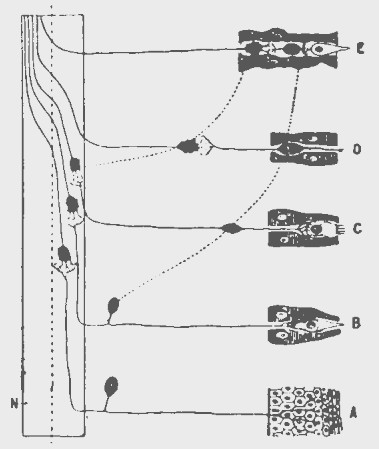
\includegraphics[scale=0.3]{./05_sensible/009}
\end{center}
Fig. 9. — Schéma des organes des sens
(D'après Gley, Traité de Physiologie, J.-B. Baillière, éd.).
\end{minipage}
\hfill
\begin{minipage}[c]{.45\linewidth}
N, centres nerveux ; A, tact; B, goût;
C, ouïe; D, odorat ; E, vue. — Les cellules 
sensorielles (absentes pour le tact et l'odorat) 
sont figurées en clair ; les neurones sensitifs
périphériques, en noir avec un noyau ; 
les neurones sensitifs centraux, en noir 
sans noyau. La ligne pointillée de droite
marque le déplacement vers la périphérie des neurones périphériques à partir de celui 
de l'audition (C) ; la ligne supérieure, le
même déplacement pour les neurones centraux à partir de celui de l'odorat (D).
\end{minipage}


%83
\section{Lois de la sensation; la Psychophysique}% 73.
Les lois de
la sensation seront donc de trois sortes, selon qu’il s’agit de ses rapports :
{\it A.} avec l’excitant; {\it B.} avec l'impression physiologique ;
{\it C.} avec les autres faits de conscience antécédents ou concomitants.

{\it A.} Lois {\it psycho-physiques}. Les premières sont les lois dites « psycho-physiques ».
1° La \textbf{\textit {loi du seuil,}} qu’on retrouvera à propos du comportement
(t. II, ch. I), s’applique à la sensation : il existe pour chaque
sens une intensité {\it minima} de l’excitant, appelée {\it intensité liminaire}
(latin : {\it limen}, seuil), au-dessous de laquelle il n’y a pas de sensation.

\vspace{0.24cm}
{\footnotesize 
La Psychologie de laboratoire s’est appliquée à déterminer ces \textsf{\textit {seuils
sensoriels,}} et l’on a pu obtenir pour chaque sens une valeur moyenne du
seuil. Mais ces valeurs n’ont rien d’absolu. Il y a naturellement des
différences individuelles. La sensibilité tactile est très inégalement répartie
selon les différentes régions du corps : très grande au bout des doigts
(2 mg à la face interne, 15 mg au dos de l'index) et à la pointe de la
langue, elle est très faible pour la peau du dos. La sensibilité visuelle n’est
pas la même pour les différentes radiations : dans des conditions moyennes
d’éclairement, elle est maxima pour une longueur d'onde de 55 µ (vers le
jaune-vert). Le goût est plus sensible à l'amer qu’au sucré. La sensibilité
olfactive varie beaucoup selon les odeurs, etc. D'autre part, par suite d'un
phénomène d'adaptation, le seuil est plus bas quand on expérimente par
{\it diminution} progressive de l’excitant que lorsqu'on le fait croître. Enfin il
faut tenir compte de la durée de l’excitation : il existe une certaine durée,
dite {\it temps utile}, au delà de laquelle seule le seuil devient invariable.}
\vspace{0.31cm}

2° La seconde loi est celle du \textbf{\textit {seuil différentiel}} : de même qu’un
excitant trop faible n’est pas senti, une {\it variation} d’intensité de l’excitant
doit atteindre un certain seuil pour qu’on sente la différence.
Les recherches poursuivies vers 1830 par le physiologiste allemand
E.-H. Weber (1795-1878) ont établi qu’{\it il existe, pour chaque espèce
de sensation, un rapport constant entre l'intensité de l’excitant initial
et la variation minima qu’il faut lui faire subir pour que la différence
soit sentie} : c’est ce qu’on appelle la \textbf{\textit {loi de Weber}} (bien qu'elle ait
été énoncée dès 1760 par le physicien français Bouguer pour les
sensations lumineuses). Autrement dit, la « constante de Weber »
qui mesure le seuil différentiel, n’est pas une valeur absolue : c’est un
rapport. Elle est, par exemple, de 1/20 pour les sensations tactiles, ce
qui veut dire que, si j’ai sur la main un poids de 20 g, celui-ci devra
être augmenté d’au moins 1 g pour que je sente la différence; mais,
si je pars d’un poids de 40 g, il devra être augmenté d’au moins
2 g. Cette loi vaut surtout pour les intensités moyennes.

Se fondant sur ces résultats, le philosophe G.-Th. Fechner (1801-1887)
crut pouvoir tirer de là une méthode de \textbf{\textit {mesure}} de la sensation,
point de départ de toute une science qu’il nomma la \textbf{\textit {Psychophysique}}
%84
(1860). Il admit ce postulat que les modifications tout juste sensibles
que subissent rios sensations quand on augmente l’excitant et qui
correspondent au seuil différentiel, sont toutes égales à la sensation
qui correspond à l'intensité liminaire, prise pour unité. Il énonça
alors la loi de Weber sous cette forme : pour que la sensation subisse
ainsi des accroissements uniformes, c’est-à-dire pour qu’elle varie
en {\it progression arithmétique} (comme les nombres 0, 1, 2, 3, etc.), il
faut faire varier l’excitant en {\it progression géométrique} (comme les
nombres 4, 10, 100, 1 000, etc.), ce qui peut encore se formuler : {\it la
sensation varie comme le logarithme de l’excitant. Ce fut la} \textbf{\textit {loi
logarithmique}} {\it ou} \textbf{\textit {loi de Fechner.}}

\begin{minipage}[c]{.45\linewidth}
Rapports de la sensation S (en ordonnées)  et de l'excitant E (en abscisses) selon 
une échelle logarithmique. Si la loi de Fechner était exacte, les accroissements 
de la sensation s'effectueraient selon la droite en pointillé Elle s'effectue en 
réalité selon une courbe en S. Mais pratiquement cette courbe coïncide avec  
la droite pour les valeurs moyennes. 
\end{minipage}
\hfill
\begin{minipage}[c]{.45\linewidth}
\begin{center}
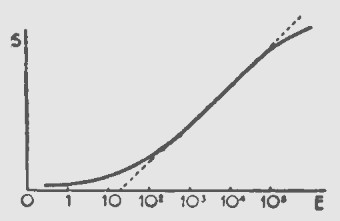
\includegraphics[scale=0.6]{./05_sensible/010}
Fig. 10. — La loi de Fechner.
(D'après Piéron, Psychologie expérimentale, (Coll. Armand Colin.)
\end{center}
\end{minipage}

\vspace{0.24cm}
{\footnotesize 
Ces conclusions de Fechner ont
été très discutées. Bergson y a
opposé une objection de principe :
les sensations, comme tous nos états
de conscience, seraient purement
{\it qualitatives}, et ce serait par une illusion matérialisante que nous
transporterions le caractère quantitatif de la cause physique ou physiologique
(intensité de l’éclairement, de l'effort musculaire, etc.) dans le domaine
de la sensation elle-même. Mais cette opposition absolue qu'établit Bergson
entre {\it quantité} et {\it qualité} est peu fondée : tout ce que la science a
appris à traduire par une quantité, et le nombre lui-même (voir le
\S 249 A), est apparu d’abord à la conscience naïve comme purement qualitatif.
— D’autres objections ont porté sur le caractère arbitraire du postulat
de Fechner. Mais toute mesure implique certaines conventions : n’est-ce
pas une convention de mesurer la vitesse d’un corps qui tombe, par l’espace
parcouru en une seconde, et cette vitesse est-elle davantage une somme de
vitesses plus petites qu'une sensation un total d'unités de sensation ?}
\vspace{0.31cm}

 



L'erreur de Fechner était ailleurs : elle était, au fond, dans la
notion même d’une « psychophysique », c’est-à-dire d’une {\it relation
directe entre l’excitant physique et la sensation comme processus conscient}.
Physicien avant d’avoir été philosophe, Fechner a méconnu en
effet qu’entre l’un et l’autre, s’intercale un intermédiaire, qui est
notre corps avec toute la complexité de ses organes, de ses voies
nerveuses, de son cerveau. La loi de Fechner exprime donc, en réalité,
un rapport entre l’excitant physique et la {\it réaction de notre sensibilité
%85
organique}, que la sensation consciente ne traduit qu’en gros et peu
fidèlement ; et en effet son graphique correct (fig. 10) donne une courbe
analogue à celle de toutesles réactions organiques (t. II, fig. 2 ). Avec ces
réserves, elle fournit une approximation suffisante pour la pratique,
et la meilleure preuve de sa valeur est qu’elle a été appliquée empiriquement
avant d’être connue scientifiquement
{\scriptsize (On sait que les premiers astronomes avaient classé les étoiles, selon leur éclat
apparent ou magnitude, en étoiles de 1r°, 2e, 3, etc., grandeur ; or cette hiérarchie
correspond en réalité à une progression géométrique décroissante : chaque classe est
2,5 fois plus brillante que celle qui la suit. — De même, les techniciens savent qu’un
gris formé de 60 p. 100 de noir ne nous donne la sensation que d'environ 20 p. 100 de
noir et qu’il faut plus de 80 p. 100 de noir pour nous donner l'illusion d’un gris moyen)}.

{\it B. Lois psycho-physiologiques}. En dehors des deux lois précédentes
qui, au fond, sont déjà des lois psycho-physiologiques, on peut énoncer
ici la loi de \textbf{\textit {spécificité des sens}} : {\it la qualité de la sensation dépend
de l'organe impressionné, et non de la qualité de l’excitant}.

\vspace{0.24cm}
{\footnotesize 
Il en résulte qu'{\it un même excitant appliqué à des sens différents détermine
des sensations différentes}, et inversement {\it des excitants différents appliqués
à un même sens provoquent la même espèce de sensation}. Tout le monde sait
qu’un choc sur l’œil provoque une sensation d’éblouissement ; une pression
sur le globe oculaire y fait apparaître des lucurs colorées appelées {\it phosphènes}.
La rupture du tympan donne lieu à une sensation de tonnerre. Si
on excite un des points de froid de la peau (voir \S 77 b) avec une pointe
portée à 45°, on éprouve une sensation de froid, et « une excitation mécanique
par pointe chaude ou froide donne sur les points de tact la seule
sensation de contact sans impression thermique » (Chauchard).}
\vspace{0.31cm}

{\it C. Lois psychologiques}. On a parfois énoncé d’autres lois concernant
le rapport de la sensation avec les autres faits psychiques qui la
précèdent ou l’accompagnent. La plus importante est la \textbf{\textit {loi de
relation}} ou \textbf{\textit {de contraste}} que Höffding
{\scriptsize (Harald Höffding (1843-1931), philosophe danois, auteur d’une Psychologie, d'une
Morale, d’une étude sur Kierkegaard et d'ouvrages intéressant la philosophie des sciences
et de la religion)}
énonçait ainsi : {\it chaque
sensation particulière est déterminée par l’ensemble et par le rapport
mutuel des différents états ou des parties d’un même état}.

\vspace{0.24cm}
{\footnotesize 
Cette relativité se manifeste à la fois quant à l'{\it intensité} apparente et
quant à la {\it qualité} de la sensation. Un bruit nous paraît plus intense au milieu
du silence, une lumière parmi l’obscurité. — Quant au contraste {\it qualitatif}, il
est surtout apparent pour les couleurs. Deux couleurs complémentaires
(c’est-à-dire dont les rayons mélangés donnent du blanc ou du gris) s’avivent
réciproquement si on les juxtapose ou si on les considère l’une après l’autre. Une
bande grise (sans contours nettement définis) sur fond coloré tend à prendre
la couleur complémentaire de ce fond. Mais le même phénomène se constate
aussi pour les autres sens, soit sous forme de contraste simultané, soit
%86
surtout sous forme de contraste successif : un mets modérément salé ou
sucré nous paraît fade après un mets qui l'était davantage ; si nous plongeons
la main gauche dans de l’eau à 45°, la main droite dans de l’eau à
15°, puis les deux mains dans une même eau à 30°, celle-ci paraît froide à
la main gauche, chaude à la main droite ; nous sommes plus sensibles au
froid en sortant d’une pièce surchauffée, etc.}
\vspace{0.31cm}

Mais, ainsi présentée, cette loi est cependant quelque peu artificielle.
Elle paraît supposer que la sensation existerait à l’état indépendant
et recevrait ensuite son intensité et sa qualité de son contexte
conscientiel. En réalité, comme on le verra plus loin, c’est {\it la notion
même de sensation isolée} qui est illusoire.

\section{Les trois sensibilités}% 74.
On distingue ordinairement cinq
sens. Mais, en réalité, l’homme possède bien plus de cinq sens et
surtout il importe de classer plus rationnellement nos diverses sensations.
Nous utiliserons ici la classification établie par Ch. Sherrington
(1857-1952) sans nous astreindre à la suivre pas à pas
{\scriptsize (Une autre classification est celle de M. Pradines qui distingue des sens du besoin
(goût, odorat, etc.), des {\it sens de la défense} (toucher) et des {\it sens supérieurs}. Mais
primordialement tous nos sens sont des sens du besoin (voir \S 79))}.
Ce physiologiste
a distingué en nous trois grands « champs » de récepteurs
sensoriels : 1° ceux des récepteurs \textbf{\textit {intéroceptifs}} qui captent les
impressions venant des surfaces intérieures de l’organisme, spécialement
du tube digestif; — 2° ceux des récepteurs \textbf{\textit {proprioceptifs,}}
qui nous renseignent sur l’activité propre de l’organisme, sur les
attitudes et les mouvements du corps; — 3° ceux des récepteurs
\textbf{\textit {extéroceptifs}} qui sont les « organes des sens » classiques et qui captent
les impressions venant des objets extérieurs. À ces trois formes de
sensibilité qui nous renseignent sur le monde « physico-chimique »,
Sherrington en ajoute une quatrième, la sensibilité \textbf{\textit {nociceptive,}} qui
est celle des récepteurs, pour les impressions douloureuses et qui nous
avertit de ce qui peut nous nuire. Mais, en tant que source de sensations
spécialisées, elle peut se rattacher au toucher.

\section{La sensibilité intéroceptive}% 75.
La première forme de sensibilité
comprend toutes les sensations qui viennent de l’estomac,
de l'intestin, celles aussi qui correspondent aux différents « besoins »:
Nous y ajouterons toutes les sensations \textbf{\textit {viscérales}} et cette sensibilité
générale du corps qu’on appelle la \textbf{\textit {cœnesthésie}} (grec : {\it koinè}, commune ;
{\it aisthèsis}, sensation). La {\it cœnesthésie} se manifeste à la conscience
par de vagues sensations d’aise ou de malaise, beaucoup plus {\it affectives}
que cognitives. Le plus souvent, chez l’homme sain, elle demeure à peu
%87
près inconsciente, recouverte qu’elle est par les autres sensations. « Il
n'y a guère que les gens malsains, a dit Maine be Biran, {\it qui se sentent
exister}. » De fait, comme l’a montré le Dr Ch. Blondel dans son
étude sur la {\it Conscience morbide}, ce n’est guère que dans les états
pathologiques ou encore dans le rêve, en un mot dans la pensée
{\it désocialisée}, réduite à la composante psycho-organique (\S 25), que la
cœnesthésie se manifeste librement.

\section{La sensibilité proprioceptive}% 76.
La seconde forme de sensibilité
est celle qui nous renseigne sur les positions, attitudes et mouvements
de notre corps et de nos membres. Ce sont :

A. Le sens \textbf{\textit {statique}} ou \textbf{\textit {labyrinthique,}} ainsi nommé parce qu’il
a son organe dans le labyrinthe (utricule, saccule, canaux semi-circulaires)
de l’oreille interne : il nous donne le sens de la verticalité
ainsi que des mouvements de rotation et de translation ; il préside à
l’{\it équilibration} générale du corps (il est en relation directe avec le
cervelet) et il joue un rôle dans le {\it sens des attitudes} ; les canaux
semi-circulaires, remplis d’endolymphe, sont d’ailleurs disposés dans
trois plans perpendiculaires correspondant aux trois dimensions de
l’espace ; lorsque nous avons tourné sur nous-mêmes et que nous
nous arrêtons brusquement, l’endolymphe continue son mouvement
par inertie : d’où la sensation du {\it vertige} ;

B. Le sens \textbf{\textit {kinésique}} ou \textbf{\textit {kinesthésique}} (grec : {\it kinèsis}, mouvement)
qui nous renseigne sur nos mouvements proprement dits, c’est-à-dire
sur les {\it déplacements} de nos membres et de tout notre corps dans
l’espace : son importance avait été mise en relief par Maine de Biran
qui avait vu dans la sensation d’{\it effort volontaire} la source de notre
distinction entre le {\it moi} et le {\it non-moi} (voir ci-dessous les \S 104 et
\S 350 A) : cette sensation correspondait, selon lui, à un influx nerveux
moteur, done centrifuge, alors que toutes les autres sensations correspondaient
à un influx nerveux sensitif, centripète ; d’où son rôle
exceptionnel. Cette interprétation a été reconnue erronée : les sensations
kinésiques ont leur origine, comme toutes les autres, dans des
terminaisons nerveuses {\it périphériques}, celles qui se trouvent dans nos
muscles, dans leurs tendons, dans le périoste des os et dans les capsules
articulaires. La simple introspection suffit d’ailleurs pour distinguer
dans la sensation globale où ils se mêlent généralement, l’élément
musculaire, l’élément tendineux, l’élément articulaire, etc. (voir
{\it Exercice} 1). Les sensations kinésiques n’en ont pas moins une grande
importance parce qu’elles se mêlent à la plupart de nos autres sensations
et qu’elles participent à la régulation du {\it tonus} musculaire ainsi
qu’à la reconnaissance des objets par la palpation (stéréognosie).
%88

\section{La sensibilité extéroceptive}% 77.
La sensibilité extéroceptive
qui nous renseigne sur les objets extérieurs, a fait l’objet d’une distinction
intéressante, due encore à Sherrington, entre les sens impressionnables
par contact direct et les sens, plus perfectionnés, qui
sont impressionnables à distance.

{\it A. Sens impressionnables par contact direct}. Parmi les premiers, il
faut placer toutes les sensibilités {\it cutanées} (tact, sens thermiques, douleur)
ainsi que les sens {\it chimiques}.

1° Le \textbf{\textit {toucher}} est le plus rudimentaire de nos sens externes puisqu'il
suppose la présence toute proche de l’objet à percevoir. Nos tissus cutanés
n’en renférment pas moins de nombreux récepteurs plus ou moins
différenciés, situés les uns dans l’épiderme, les autres dans les parties
profondes de la peau (terminaisons libres des nerfs, corpuscules de
Pacini, de Krause, de Meissner), de sorte que le « toucher » commun
se divise, en réalité, en quatre sens distincts au moins : le {\it tact} proprement
dit, le sens du {\it chaud}, le sens du {\it froid}, le sens de la {\it douleur}
{\scriptsize (L'exploration fine de la peau montre l’existence de points sensibles à chacune de
ces quatre impressions (voir $\beta$). L'observation clinique confirme ces données et prouve
l'{\it indépendance relative de ces quatre sens} : dans un membre « engourdi », le tact disparaît
le premier, puis les sensations thermiques, tandis que le sens de la douleur est hyperexcité ;
certains anesthésiques (novocaïne) abolissent la douleur et la sensibilité au
froid, mais laissent subsister le tact ; dans la régénération progressive de la sensibilité,
la douleur reparaît la première puis les impressions thermiques, et, en dernier, le tact.
Enfin le {\it temps de réaction} (voir chap. XXIV) n’est pas le même pour ces diverses sensations
(d’après Chauchard))}.

$\alpha$. Le \textbf{\textit {tact}} proprement dit est essentiellement le sens des {\it contacts}
et des {\it pressions}. Les contacts intéressent surtout la sensibilité superficielle,
celles des « points de tact », plus précise et plus fine (sensibilité
{\it épicritique} de H. Head). Les pressions intéressent surtout les
régions profondes de la peau (sensibilité {\it protopathique}) et provoquent
des sensations beaucoup moins bien localisées et plus vagues, apparentées
à la sensibilité intéroceptive. — Il y a lieu de bien distinguer
le tact proprement dit du \textbf{\textit {toucher actif}} ou toucher de palpation,
qui implique des mouvements de la main et des doigts, donc des
sensations kinésiques (476 B),et qui est à l’origine de sensations
complexes telles que celles du {\it lisse} et du {\it rugueux}, du {\it soyeux} et du
{\it velouté}, du {\it sec} et de l’{\it humide}, du {\it graisseux}, du {\it visqueux}, etc.

$\beta$. Les sensations \textbf{\textit {thermiques}} correspondent à des points sensibles,
les uns au {\it froid}, les autres au {\it chaud}, les premiers (de beaucoup les
plus nombreux) étant situés à la limite de l’épiderme et du derme, les
seconds dans les régions profondes du derme. Il est facile, en promenant
sur la peau une pointe chaude ou froide, de discerner des points
%89
où l’on ne sent que le contact, d’autres où l’on sent le froid, d’autres
enfin où l’on sent le chaud.

$\gamma$. Enfin le physiologiste allemand von Frey (1891) a établi l’existence
de « points de douleur » ou récepteurs \textbf{\textit {algiques}} (grec : {\it algos},
douleur) qui correspondent à des terminaisons libres des nerfs dans
l’épiderme et qui donnent notamment la sensation de {\it piqûre}. On
reviendra sur la question au chapitre III du tome II.

2° Les \textbf{\textit {sens chimiques}} proprement dits sont le {\it goût} et l’{\it odorat}. Ils
sont intimement liés aux fonctions de nutrition et l’on a pu dire
qu’ils sont les « agents de liaison entre le chimisme de l’être et le
chimisme de son aliment » (Fr. Houssay).

$\alpha$. Le goût a pour organes les {\it bourgeons gustatifs} qui se trouvent
dans les papilles de la langue, notamment les papilles caliciformes
formant le V lingual et il nous donne les quatre sensations fondamentales
de l’{\it amer}, du {\it sucré}, de l’{\it acide} et du {\it salé}. Toutes les autres sensations
que nous attribuons ordinairement au goût, sont ou composées
(le {\it fade} est un mélange de sucré et de salé) ou même mêlées d’impressions
provenant des autres sens, en particulier de l’{\it odorat} (lorsqu'on
est enrhumé ou qu’on se bouche les narines, les aliments nous semblent
perdre beaucoup de leur saveur), voire du {\it tact} (velouté d’une sauce
ou d’un vin, saveurs farineuses, gommeuses, etc.) ou des sens {\it thermiques}
(fraîcheur d’une boisson, d’une glace, etc.).

$\beta$. On serait tenté de classer l’\textbf{\textit {odorat}} parmi les sens impressionnables
à distance. Mais, en réalité, il est intimement lié au goût, et les
{\it cellules olfactives}, situées dans la muqueuse de la partie supérieure
des fosses nasales, sont impressionnables par le contact direct des
molécules gazeuses provenant des corps odorants. On a tenté diverses
classifications des odeurs. Mais ces classifications sont purement
subjectives, car on connaît mal la relation entre composition chimique
et odeur. Les odeurs « piquantes » mettent en jeu la sensibilité {\it tactile}
ou même {\it algique} (alcali) des muqueuses nasales. Mais il faut surtout
remarquer ici l’infériorité de l’homme quant au développement de ce
sens : la plupart des animaux sont mieux doués que lui sous ce
rapport, et l’odorat joue un grand rôle dans le comportement, non
seulement des Mammifères, mais aussi des Insectes.

{\it B. Sens impressionnables à distance}. Sherrington a mis en lumière
l’importance de la \textbf{\textit {sensibilité à distance}} pour le développement psychique.
Plus indépendants du milieu extérieur que ceux qui exigent
le contact direct, ces sens qui sont l’{\it ouïe} et la {\it vue}, apportent en effet
à l’être vivant des messages lointains et lui permettent ainsi une
{\it adaptation anticipée} de son comportement.

$\alpha$. Le sens de l’\textbf{\textit {ouïe}} est impressionné par les vibrations de l'air,
%90
périodiques (sons) ou irrégulières (bruits), qui par l’intermédiaire du
tympan et de la chaîne des osselets, viennent agir sur l’organe de
Corti, relié au nerf auditif. Les impressions auditives nous permettent
de distinguer subjectivement l'{\it intensité} des sons qui, physiquement,
dépend de l'amplitude des vibrations, leur {\it hauteur} qui dépend de la
fréquence, et leur {\it timbre} qui dépend de sons accessoires, les harmoniques,
qui viennent s’ajouter au son fondamental.

$\beta$. Le sens de la \textbf{\textit {vue}} est impressionné, chez l’homme, par les
radiations lumineuses de 0,39 µ à 0,82 µ qui, à travers les différents
milieux de l’œil, viennent agir sur la {\it rétine}. On sait que celle-ci est un
épanouissement du nerf optique comprenant jusqu’à dix couches
de fibres et de cellules, dont la plus importante est celle qui renferme
les {\it cônes} et les {\it bâtonnets}, prolongements des cellules visuelles. Les
bâtonnets sont surtout abondants à la périphérie, tandis que la « tache
jaune » n’est formée que de cônes. Les premiers, adaptés à la vision
crépusculaire, ne nous donnent que des sensations de {\it lumière} ; les
seconds, moins sensibles, mais adaptés à la grande luminosité, nous
donnent en même temps des sensations de {\it couleur}.

\vspace{0.24cm}
{\footnotesize 
La sensibilité aux couleurs peut faire totalement défaut : c’est
l’{\it achromatopsie} ; elle peut manquer seulement pour certaines couleurs, par exemple
le vert et le rouge (le rouge paraît alors noir, et le vert gris clair) : c’est le
{\it daltonisme}. L'enfant qui distingue la lumière et l'ombre dès la fin de la
première semaine, ne semble percevoir d’abord que le rouge et le jaune ; il
ne perçoit et surtout n’identifie le vert, le bleu, le violet que beaucoup plus
tard. On a remarqué que les textes très anciens (Védas, Avesta, Ancien
Testament, Homère) ne font pas mention de ces dernières couleurs, et
certaines races comme les Annamites, les distinguent fort mal (les indigènes
des îles Torrès, si l’on en croit Rivers, les confondent complètement).}
\vspace{0.31cm}

\section{Valeur des différents sens}% 78.
On a déjà remarqué (\S 72)
qu’au point de vuc mème de leur structure anatomique, nos sens
semblent présenter une certaine {\it hiérarchie}. Cette hiérarchie se vérifie si
l’on considère la valeur des messages qu’ils nous apportent. — {\it A.} En
ce qui concerne d’abord leur \textbf{\textit {finesse,}} les différences sont énormes.
La sensibilité {\it intéroceptive} et la cœnesthésie surtout ne nous fournissent
guère que des renseignements vagues et grossiers Nous avons
noté que la cœnesthésic est plus affective que cognitive : or certains
auteurs ont posé cette loi que, dans la sensation, {\it l'élément affectif et
l'élément cognitif varient en raison inverse l’une de l’autre}. Formule un
peu étroite sans doute, mais qui exprime cependant un fait réel : les
sens supérieurs, si riches en informations sur le monde extérieur,
sont relativement peu affcctifs par eux-mêmes. Une couleur peut
certes être agréable ou désagréable et surtout plus ou moins dynamogénique
%91
(\S 78 D), mais son intensité affective n’a rien de comparable
à celle d’une douleur interne par exemple. La sensibilité
{\it proprioceptive} est déjà plus fine : ce qu’on appelle l'adresse manuelle
tient à la précision des mouvements, guidée elle-même, en partie, par
la finesse des sensations kinésiques. Quant aux sens {\it externes}, ils
sont souvent d’une finesse remarquable (voir les chiffres dans
Chauchard).

\vspace{0.24cm}
{\footnotesize 
La finesse des sens ne consiste pas seulement d’ailleurs dans leur sensibilité
liminale, mais aussi dans leur \textsf{\textit {acuité,}} c’est-à-dire leur pouvoir de
{\it discrimination} entre deux impressions voisines. L’{\it acuité tactile} qui se
mesure avec le « compas de Weber » est la plus petite distance à laquelle deux
contacts sont sentis comme distincts sur la peau : or, de 45 mm sur la
poitrine, elle descend à 2 mm à l'extrémité des doigts. On mesure de même
l'{\it acuité auditive} (différence minima de hauteur entre deux sons), l’{\it acuité
visuelle} (distinction de deux points lumineux rapprochés, ou encore appréciation
des différences d'intensité, ou bien de fréquence entre les radiations :
l'œil humain est sensible à 750 échelons de luminosité distincts).}
\vspace{0.31cm}

{\it B.} Quant à l'{\it importance} des renseignements qu’ils nous apportent,
les sens s’échelonnent de façon analogue (sur le rôle de l'intuition
sensible dans la connaissance, voir ci-dessus, \S 60). Les sens {\it intéroceptifs}
ne sont guère que des avertisseurs, et qui ne sont pas toujours
très fidèles. — Le sens {\it kinésique}, mêlant ses impressions à celles de la
plupart des autres sens, est déjà plus précieux : ce sont, par exemple,
les mouvements de la main, les mouvements de l’appareil oculaire
qui nous aident à apprécier les distances (\S 94). Le {\it goût} et l’{\it odorat}
renseignent le chimiste, le pharmacien, le dégustateur en vins, plus
rapidement et parfois mieux qu’une analyse chimique. L’{\it ouïe} qui,
pour l’animal, est surtout un avertisseur (\S 79), a pris pour l’homme
une importance exceptionnelle du fait de l’existence du langage articulé,
du rôle social de la parole et de l’invention de la radio.

Mais c’est évidemment la {\it vue} qui nous apporte le plus de renseignements
sur le monde extérieur, d'autant plus qu’elle est à la fois :
1° un sens {\it à très longue portée} : on raconte que des voyageurs perdus
dans les Andes aperçurent à une énorme distance l'expédition qui
venait à leur secours ; 2° un sens {\it synthétique}, qui nous donne d’emblée
les objets dans leur totalité tandis que le toucher est analytique
(l’aveugle est obligé de palper successivement les diverses parties
d’un objet nouveau pour s’en faire une idée). Même dans le domaine
de la pensée abstraite, il y a souvent avantage à présenter sous forme
de tableaux synoptiques, de diagrammes, etc., qui « parlent aux yeux »,
une représentation systématisée d’un ensemble de données.

{\it C.} Des remarques parallèles s’appliquent à la valeur \textbf{\textit {esthétique}}
%92
des différents sens. L'art est essentiellement désintéressé. Aussi les
sens inférieurs qui sont trop étroitement liés à nos fonctions organiques,
ne sont-ils guère susceptibles de valorisation esthétique. C’est
ainsi qu’on ose à peine parler d’un art proprement dit s’adressant au
sens du {\it goût}. Le sens de l’{\it odorat} prêterait également à discussion :
n’existe-t-il pas cependant un « art des parfums » ? Il en va déjà
autrement du {\it toucher} qui, au moins par association avec d’autres
sens, peut prendre une valeur spécifiquement esthétique : une pianiste
contemporaine a affirmé que «nous pouvons arriver à mieux sentir
la beauté de la musique avec nos doigts qu’à travers notre oreille ».
Il n’est pas douteux que, dans les arts plastiques, le {\it toucher actif} n’ait
bien une valeur esthétique par lui-même : Michel-Ange devenu aveugle
se faisait conduire devant ses œuvres sculpturales pour en palper les
formes. Mais ce sont surtout les deux sens supérieurs, l’{\it ouïe} et la
{\it vue} qui sont proprement esthétiques. Il y a même une sorte de
{\it sensualité esthétique} de l’oreille et de l’œil : à la base de la musique, n’y
a-t-il pas une valeur accordée à certaines sonorités, à certains accords
pour eux-mêmes, de même que, chez certains peintres comme Véronèse,
Rubens, Delacroix, il existe un goût de la couleur pour elle-même?
Encore faut-il, comme l’a observé M. Pradines, que le son ou la
couleur, pour être goûté esthétiquement, soit en quelque sorte
détaché de l’objet et devienne lui-même son propre objet. Quoi qu’il
en soit, c’est à ces deux sens que s'adressent tous les {\it arts} proprement
dits : mais, tandis que l’art de l’audition est unique, — c’est la
musique, — les arts qui s’adressent à la vue sont multiples : ce sont
tous les « arts du dessin » : peinture, gravure, sculpture, architecture,
et, pour une part, les arts du spectacle : théâtre, chorégraphie
et, quand il veut bien se soucier de valeurs esthétiques, le
cinéma.

{\it }D. On peut encore parler d’une valeur {\it dynamogénique} des sensations
externes. Déjà certaines odeurs sont stimulantes, d’autres alanguissantes
ou écœurantes. Certains sons sont tristes et déprimants,
d’autres joyeux et excitants : n’a-t-on pas, dans certains ateliers
industriels, utilisé la musique comme stimulant du travail? Mais ce
sont surtout les {\it couleurs} qui jouissent de telles propriétés.

\vspace{0.24cm}
{\footnotesize 
Le rouge accélère le cœur et possède un pouvoir excitant ; l’orangé a des
vertus toniques et crée l’euphorie ; le vert est reposant et produit une sensation
de fraîcheur ; le bleu favorise le sommeil, mais donne une impression
de froid ; l’indigo et le violet engendrent la mélancolie. Ces actions sont si
nettes qu’on en tient compte aujourd’hui dans la « peinture fonctionnelle »
pour les ateliers, les salles d'hôpital ou de clinique, les intérieurs d’avion, etc.
Outre l’action directe sur le système nerveux, il se peut qu’il y ait là un
%93
phénomène de «conditionnement» : l’orangé évoquerait par exemple
l’action du soleil. C’est probablement le cas pour le « noir-rouge » dont
parle quelque part Van Gogh (voir {\it Exercice} 4).}
\vspace{0.31cm}

\section{Rôle de la sensation}% 79.
Nous comprendrons mieux la véritable
valeur de la sensation si nous cherchons à préciser sa \textbf{\textit {nature}}
et son \textbf{\textit {rôle}} dans notre vie mentale. Par un préjugé à la fois réaliste
et intellectualiste, le sens commun considère la sensation comme une
sorte de {\it réplique}, de {\it copie}, dans notre esprit, de l’objet perçu. Or
l'esprit n’est pas un miroir, et les lois de la sensation montrent qu’il
n’y a pas parallélisme parfait entre l’excitant, quel qu’il soit, et l’état
de conscience qu’il suscite. La {\it loi de spécificité}, en particulier, nous
rappelle que la sensation dépend de l'appareil récepteur, de l'organe
sensoriel : les animaux qui ont des organes différents des nôtres, perçoivent
les choses tout autrement que nous
{\scriptsize (L'oreille du chien est sensible aux ultra-sons (de même que celle de la
chauve-souris), et son odorat saisit des odeurs que nous ne sentons pas. Les yeux composés
des insectes leur donnent une vision du monde toute différente de la nôtre ; la plupart
d’entre eux ne voient, parmi les couleurs, que le jaune et le bleu ; mais les fourmis sont
sensibles à l’ultra-violet. Etc)},
et, même dans l’espèce
humaine, l’étendue de la sensibilité des différents organes varie selon
les races
{\scriptsize (On a vu que les Annamites discernent mal certaines couleurs de fréquence
élevée. Chez certains Nord-Africains, l'oreille est sensible aux ultra-sons)}.

La {\it loi de relation} peut s’interpréter en disant que nous
sommes surtout sensibles aux {\it différences} ou aux {\it rapports}, à ce qui
{\it change}, à ce qui {\it varie}, plutôt qu’à ce qui reste constant : ainsi, nous
ne sentons pas les températures, mais les différences de température
entre le milieu extérieur et notre corps ; aussi sommes-nous beaucoup
plus sensibles au froid quand nous avons la fièvre.

C’est que nos sens ne sont pas des instruments de {\it connaissance}
désintéressés. Il faut leur appliquer la conception \textbf{\textit {biologique}} indiquée
au \S 31 D. On se rappelle que, selon cette conception, la conscience
a primordialement une fonction {\it vitale}. La sensation doit donc
avoir d’abord, elle aussi, un rôle {\it vital} : « les sensations constituent
des \textbf{\textit {symboles biologiques}} des forces extérieures agissant sur l’organisme,
mais qui ne peuvent avoir avec ces forces plus de ressemblance
qu’il n’y en a entre ces sensations mêmes et les mots qui
les désignent dans le système symbolique du langage (H. Piéron) ».
Les Cartésiens, en dépit de leur intellectualisme, l’avaient parfaitement
compris : « Les objets qui meuvent les sens, écrit DESCARTES,
n’excitent pas en nous diverses passions [impressions] à raison de
toutes les diversités qui sont en eux, mais seulement en raison des
diverses façons qu’ils peuvent nous nuire ou profiter », et plus explicitement
%94
encore Malebranche : « Nos sens ne nous sont donnés que
pour la conservation de notre corps. » Or, de ce point de vue, ce qui
intéresse surtout l’être vivant, ce sont les {\it variations} du milieu extérieur,
parce qu’elles exigent une réadaptation. Ainsi s'expliquent les
caractères qu’expriment les lois de la sensation. La loi de Weber
elle-même doit s’interpréter de la sorte : ce qui nous importe pratiquement
dans les choses, « c’est moins leur éclairage ou leur obscurité, leur
force ou leur faiblesse sonore {\it d’une façon absolue} que la netteté avec
laquelle elles tranchent dans leur ensemble et dans leurs parties les
unes sur les autres et que la grandeur des différences que nous y
percevons ».

Mais la même réserve s'impose ici que celle que nous avions for:
mulée à la fin du \S 31. De même qu'il a su faire de la conscience un
instrument de connaissance désintéressée, l’homme a su conférer à
ces {\it avertisseurs vitaux}, à ces {\it signaux subjectifs} que sont les sensations
une valeur {\it intellectuelle} et {\it esthétique}. La sensation peut devenir instrument
intellectuel, moyen de {\it connaissance} à condition d’être \textbf{\textit {interprétée,}}
et cette interprétation est à deux degrés : elle peut se faire
sur le plan de la connaissance vulgaire (voir ci-dessus, \S 54),et c’est
la {\it perception} commune ; elle peut se faire aussi sur le plan de la connaissance
{\it scientifique} où elle devient, en quelque sorte, une interprétation
au second degré : une tache rouge sur du papier de tournesol révèle
au chimiste que le liquide dont une goutte est tombée sur le papier
est un acide. — Pareillement, l’homme a fait de ses sens primitive
ment tout utilitaires des instruments de jouissance {\it esthétique}. Pour
l'animal, l’ouïe n’est qu’un avertisseur qui l’informe de l'approche
d'un danger, du passage de la proie, etc. Pour l’homme, il est
devenu l'instrument du plus merveilleux des arts : la musique.

\section{La notion de « sensation »}% 80.
Nous avons traité jusqu'ici
de la sensation, tout en tenant compte dans une certaine mesure, de
son environnement physiologique et psychique, comme si elle était
isolée. Le moment est venu de {\it mettre en question} cette façon de voir
et, avec elle, {\it la notion de sensation elle-même}. On a été jusqu’à dire que
« la sensation est une pure rêverie de psychologues ». Tout au moins,
faudrait-il dire avec M. Merleau-Ponty (1908-1961) que, « loin d’être
un contenu primitif et élémentaire de la conscience, la sensation,
c'est-à-dire l'appréhension d’une pure qualité, est un mode d’organisation
tardif et exceptionnel de la conscience humaine... Ce qui est premier
chronologiquement dans le comportement comme dans la perception
ce nest ni une mosaïque de parties extérieures, ni l’unité précise que
rend possible l'analyse : c’est, comme on l’a dit souvent, le syncrétisme ».
%95
La qualité, en effet, « n’est pas un élément de la conscience,
c’est une propriété de l’objet » : le rouge et le vert, par exemple, ne
sont pas des {\it sensations}, ce sont des {\it sensibles} qui font tableau devant
moi et ne sont donc pas moi. Par suite, la sensation ne peut être qu’un
« produit de la pensée tournée vers les objets », donc « le dernier terme
de la représentation du monde ». Les {\it perceptions de fait les plus simples}
que nous connaissions, même chez les animaux, « portent sur des
relations, et non sur des termes absolus», non sur des objets
{\scriptsize (M. Merceau-Ponry allègue, à l’appui, les expériences de KômLer où des poules
sont dressées à choisir, de deux tas de grains égaux, l’un signalé par un gris clair G 1,
l’autre par un gris moyen G 2, celui qui est le plus clair (G 1). Au bout de 500 épreuves,
la réaction étant acquise, on remplace G 2 par un troisième G 0 plus clair que G1 :
G1 est alors abandonné, et c’est G 0 qui est choisi le plus souvent. De même, si l’on
conserve G 2 ct si l’on remplace G 1 par un autre tas G 3, signalé par un gris foncé,
c'est alors G 2 qui est choisi. Les animaux choisissent donc « le plus clair » des deux tas
présentés : ils se guident d’après une relation. — De même, des rats, dressés à distinguer
une cntrée pcinte en noir qui conduit à la nourriture d’unc entrée peinte en gris, choisissent
régulièrement la plus foncée si l’on remplace le noir et le gris par du rouge et du
rose. — Ces faits sont, à notre avis, à rapprocher des {\it perceptions syncrétiques} dont il sera
question au \S 83)}.

Il y a ici à distinguer, croyons-nous, bien des thèses différentes. —
1° Qu’il n’existe pas dans la conscience de sensations {\it isolées}, que,
même (et peut-être surtout) chez le nouveau-né, un bruit, une
lueur, etc., ne fassent qu’introduire un incident épisodique dans l’ensemble
indistinct de son état d’âme à un moment donné, c’est ce que
nous ont déjà appris la description jamésienne du « courant de conscience »
ou les protestations bergsoniennes contre le {\it morcelage} artificiel
qui nous fait découper dans la mouvance continue de la durée
des « états » inertes et indépendants (\S 37). —2° Que d’autre part
nous percevions des {\it différences} ou des {\it relations} (sans cependant qu’il
y ait, à proprement parler, {\it prise de conscience des rapports}) plutôt
que des qualités absolues ou des objets, c'est ce que nous avons
déjà remarqué et expliqué par le rôle biologique de la sensation (\S 79).
— 3° Qu’enfin « ce qui est premier chronologiquement », ce ne soit
pas une mosaïque d’éléments comme l’avait admis l’atomisme psychologique
(\S 37 {\it fin}), mais bien un {\it syncrétisme} où se trouve encore
uni ou plutôt confondu ce qui sera plus tard distingué, c’est ce que
nous avons indiqué comme une des caractéristiques mêmes de la
pensée enfantine (\S 40). — 4° Mais déjà se fait jour ici une certaine
équivoque. Dire que la pensée débute par le {\it syncrétisme}, ce n’est pas
dire que la perception sensible soit d'emblée {\it structurée} et {\it organisée}.
Nous reviendrons là-dessus en discutant le {\it Gestaltisme} (\S 81-82 et
83 {\it A}). — 5° Est-il vrai, d’autre part, que cette perception ne nous
donne jamais de {\it qualités pures}, mais que toute qualité soit {\it objet} et
objet déjà doué de signification, qu’il n’y ait pas par exemple de
%96
rouge pur, mais que tel rouge soit « le rouge laineux d’un tapis » ou
le rouge de telle toile d'Henri Matisse ? Nous craignons qu’il y ait
là {\it confusion de deux plans de conscience} (chap. III) très différents
et que notre langage {\it qui est le langage de l’adulte, voire le langage
philosophique, qui suppose donc déjà effectuées des opérations ou des
distinctions qui précisément ne le sont pas encore aux plans inférieurs
de la pensée}, n’aide à cette confusion.

\vspace{0.24cm}
{\footnotesize 
Certes, pour l'{\it adulte}, tout bruit, toute forme colorée ont d'emblée une
signification : c’est ce que montrait l’exemple cité au \S 71. Mais est-il sûr
qu’il y a bien là quelque chose d'{\it originel} ? Certains sens, comme l’odorat,
peut-être le toucher, sans parler bien entendu des sens intéroceptifs, ne
nous fournissent-ils pas encore parfois des sensations purement qualitatives,
sans signification déterminée ? Et pourquoi dès lors n’en aurait-il pas été
de même des sens supérieurs à l’origine? {\it La chirurgie du cerveau a d’ailleurs
permis d'établir expérimentalement}, conformément à la distinction indiquée
au \S 29 {\it B} entre les zones sensitives et les zones gnosiques, {\it qu’en excitant
électriquement certains points de l'écorce, on provoque des sensations pures}
(par exemple, couleurs), tandis qu’ailleurs l’excitation provoque des
perceptions et des images. Même équivoque quand on nous dit que les qualités
sensibles sont nécessairement perçues comme propriétés de l’objet. Certes,
dans le syncrétisme primitif, elles ne sont pas perçues comme sensations
purement subjectives. Mais on a déjà vu au \S 44 (et l’on verra mieux encore
au chapitre suivant) que la pensée proprement objective, la prise de conscience
{\it de l’objet comme tel} ne sont nullement incluses dans la sensation.}
\vspace{0.31cm}

6° Nous touchons ici à l'illusion majeure, l'illusion d’\textbf{\textit {immédiateté}}
(voir ci-dessus le \S 58). — La Phénoménologie prétend revenir à
« l’expérience directe », au « contact immédiat avec la réalité ». Mais,
observe M. Pradines, « l'immédiat et le primitif est précisément
ce qui ne peut jamais être {\it donné}, ayant servi à faire tout ce qui est
donné », et plus explicitement encore D. H. Salman
{\scriptsize (Dans la Revue philosophique de Louvain, mai 1952)} :

\vspace{0.24cm}
{\footnotesize 
« La seule expérience totalement immédiate et entièrement naïve serait
celle du nouveau-né. Dès la naissance en effet, commence un processus d’élaboration
et de croissance perceptuelles, dont la Psychologie génétique fait
connaître les étapes. Conditionnées par toutes les expériences personnelles
du sujet, par les pressions de l’adulte, les déterminismes de la langue, de
l’enseignement et de la société, les fonctions cognitives subissent un développement
dont la linguistique, la caractérologie et l’ethnologie comparée
révèlent les multiples possibilités. Toutes les manières de percevoir, de
classifier, de catégoriser... sont élaborées au cours de ce développement et
elles se diversifient à l'extrême suivant les milieux culturels considérés. »}
\vspace{0.31cm}

\section{La perception des « formes »}% 81.
Est-ce à dire cependant
que la sensation ne nous fournisse que des éléments isolés, comme on
le croyait autrefois? C’est ici que la théorie de la Forme ({\it Gestalt-theorie})
%97
énoncée par Ehrenfels (1859-1932), Wertheimer (1880-1943),
Koffka (1886-1941), Lewin (1890-1947), Köhler (né en 1887),
etc., apporte un point de vue nouveau. D’après cette théorie, la perception
sensible nous donne immédiatement, indépendamment de toute
expérience préalable et de l'intervention de la mémoire, certaines
« formes » ({\it Gestalten}), c’est-à-dire certains \textbf{\textit {ensembles structurés :}}
« {\it Les structures sont des caractères immédiats du donné au même titre que
leur contenu} » (Köhler). Elles ne sont donc pas constituées par synthèse
d'éléments préexistants : ce sont au contraire « les éléments sensoriels
eux-mêmes qui sont déterminés par les caractères et les propriétés
du tout ». Autrement dit, à l’ancienne réduction atomiste, le {\it Gestaltisme}
substitue une interprétation qui est toujours fonction d’un
{\it champ perceptif} total. Les « formes » sont immanentes au donné sensible ;
elles sont des propriétés, non seulement de la vie psychique,
mais déjà du monde physiologique et même physique. Les lois de
structuration du champ sont donc des lois d'{\it équilibre physique} qui
régissent les courants nerveux déclenchés par le contact psychique
avec les objets extérieurs et par ces objets eux-mêmes, le tout formant
un circuit global.

\vspace{0.24cm}
{\footnotesize 
Ces conceptions ont conduit à de nombreux travaux expérimentaux
d'où les « gestaltistes » ont tiré les lois suivantes : 1° une loi générale de
\textsf{\textit {prégnance,}} d’après laquelle, parmi toutes les structures possibles (par
exemple, parmi toutes les apparences possibles d’un dessin), il y en a une
qui est {\it prédominante}, qui s'impose de préférence aux autres ; — 2° les lois
de la \textsf{\textit {ségrégation des unités}} : dans l’ensemble du champ, certaines unités
perceptives se constituent {\it spontanément} selon des lois : 

\begin{minipage}[c]{.45\linewidth}
{\it a.} de {\it proximité}
des éléments : ainsi, dans la figure 11 A, on voit tout de suite des colonnes
verticales formées de deux rangées de points {\it a-b, c-d, e-f,} tandis que, si
l’on augmentait la distance {\it ab} et diminuait la distance {\it bc} (le dessin est à
la limite), cette structure cesserait de s'imposer; {\it b.} de {\it similitude} entre
les éléments : ainsi, la figure 11 B apparaît d'emblée comme formée de
quatre tronçons comprenant des éléments semblables ; {\it c.} de {\it direction commune}
des éléments : la figure 11 C se présente spontanément comme une
oblique sur une droite horizontale, et non comme un ensemble de tirets ;
\end{minipage}
\hfill
\begin{minipage}[c]{.45\linewidth}
\begin{center}
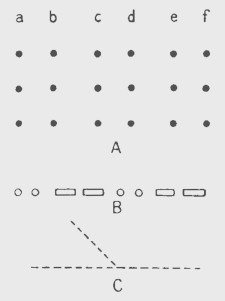
\includegraphics[scale=0.6]{./05_sensible/011}

Fig. 11. Ségrégation des unités
\end{center}
\end{minipage}


— 3° la loi de \textsf{\textit {la bonne forme}} : la forme « prégnante » est toujours « la meilleure»,
c’est-à-dire celle qui présente « le maximum d'unité, de simplicité, de régu-
larité », la mieux structurée, la moins compliquée, la plus symétrique, etc.


\begin{minipage}[c]{.45\linewidth}
\begin{center}
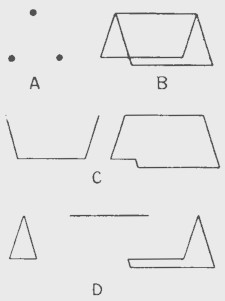
\includegraphics[scale=0.6]{./05_sensible/012}

Fig. 12. La loi de la « bonne forme ».
\end{center}
\end{minipage}
\hfill
\begin{minipage}[c]{.45\linewidth}
Dans la figure 12 A, nous apercevons immédiatement les trois sommets
d’un triangle, et non trois points quelconques ; dans la figure 12 B, deux
parallélogrammes ayant un côté commun, et non un assemblage de figures
compliquées telles que celles des figures 12 C ou 12 D qui pourraient également
la composer.
\end{minipage}


— 4° les lois \textsf{\textit {de la figure et du fond}} : dans un champ
hétérogène, apparaît généralement comme figure : {\it a.} ce qui a un {\it contour}
déterminé, par opposition au fond qui n’en a pas; {\it b.} ce qui est {\it articulé,
différencié,} par opposition au fond qui est plus homogène, plus uniforme ;
{\it c.} ce qui est {\it enveloppé} par le fond : 

\begin{minipage}[c]{.45\linewidth}
\begin{center}
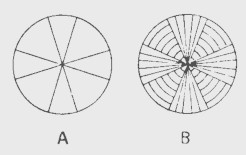
\includegraphics[scale=0.7]{./05_sensible/013}
\end{center}
\end{minipage}
\hfill
\begin{minipage}[c]{.45\linewidth}
\begin{center}
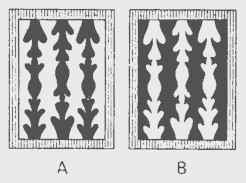
\includegraphics[scale=0.7]{./05_sensible/014}
\end{center}
\end{minipage}
\begin{center}
Fig. 13 et 14. Lois de la figure et du fond.
\end{center}

la figure 13 A est vue comme une croix
%98
à bras minces sur un fond représenté par les secteurs plus ouverts ; {\it d.} ce qui
correspond à certaines {\it directions privilégiées} de l’espace : dans la figure 13 A
l'horizontalité et la verticalité des bras s’ajoutent à l'influence précédente ;
c'est plus net encore dans la figure 13 B où les secteurs sont égaux (remarquer
qu’on a même l'impression, en ce cas, que le fond de cercles concentriques
se continue sous la croix) ;
 {\it e.} ce qui a une structure symétrique par
opposition au fond, qui est asymétrique : dans la figure 14 A, ce sont les
parties noires qui se détachent sur fond blanc parce que leurs contours
%99
sont symétriques par rapport à un axe vertical tandis que, dans la figure 14 B
ce sont les parties blanches qui se détachent sur fond noir pour la même
raison ;

— 5° la loi de transposition : la « forme » peut toujours être « transposée »,
telle une mélodie (exemple cité par Ehrenfels) que l’on reconnaît
facilement malgré une transposition qui change toutes les notes. La transposition
démontre que le tout, comme il a été dit ci-dessus, est indépendant
par rapport aux éléments.
\begin{center}
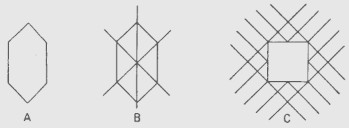
\includegraphics[scale=1.3]{./05_sensible/015}

Fig. 15. — Permanence et camouflage des « formes ».
\end{center}
 D'une façon générale, la « forme » demeure tant
qu’on y introduit des modifications qui n’altèrent pas sa structure primitive
(fig. 15 A et B). Si au contraire on ajoute à une figure des lignes qui
en changent complètement la structure (fig. 15 C), celle-ci n'est plus perçue
dans l’ensemble du dessin, bien qu'elle y soit toujours, parce que d'autres
structures en ont pris la place (carré sur fond quadrillé).}
\vspace{0.31cm}

\section{Discussion du Gestaltisme}% 82.
C'est surtout par réaction
contre l’atomisme psychologique (\S 37) que la Psychologie de la forme,
en tant que {\it psychologie des ensembles}, a connu un très grand succès.
Il y a peut-être cependant un faux dilemme dans l’opposition : ou
bien atomisme des sensations isolées, ou bien « totalités ». Ainsi que
le remarque J. Piaget, « il y a en réalité trois termes possibles : ou
bien une perception est une synthèse d'éléments, ou bien elle constitue
une totalité d’un seul tenant, {\it ou bien elle est un système de rapports} ».
Chaque rapport devient alors lui-même, si l’on veut, une
totalité, mais la totalité d'ensemble devient analysable sans qu'on
soit, pour autant, obligé d’en revenir à l’atomisme, « Cela dit, rien
n'empêche de concevoir les structures totales comme le produit d’une
{\it construction} progressive, procédant, par différenciations accommodatrices
et assimilations combinées, ni de mettre cette construction
en rapport avec une intelligence douée d'activité réelle par opposition
au jeu des structures préétablies » (Piaget).

{\it A.} Un des inconvénients majeurs du Gestaltisme est en effet qu’il
réduit excessivement le rôle de l'{\it activité de l'esprit}. Il prétend tout
ramener à des lois \textbf{\textit {physiologiques}}, réduites elles-mêmes à des lois
%100
d'équilibre \textbf{\textit {physique.}} Köhler admet par exemple que la « forme »
est donnée toute faite dans les perceptions élémentaires grâce à certaines
dispositions anatomiques des nerfs sensitifs (existence de fibres
transversales, etc.). Il y aurait ainsi un {\it principe d’isomorphisme},
d’après lequel, à tout ensemble psychique tel que la perception, correspond
un ensemble physiologique (circuit global de l’objet au cerveau
par les sens). Or il n’y a là qu'hypothèses et « physiologie fantaisiste »
(Janet) imaginée pour les besoins de la cause (tout comme
l'avait fait jadis l’associationnisme). Le « principe d’isomorphisme »
ne fait que restaurer sous sa forme la plus discutable le vieux parallélisme
psycho-physiologique (\S 31 C). Le tout se fonde sur « une
conception vraiment trop simpliste des mécanismes cérébraux » (Piéron) :
si certains phénomènes physiologiques sont ramenés aujourd’hui
à des modèles physiques, il s’en faut qu’ils le soient tous. En
réalité, les faits allégués ne peuvent s'interpréter que du point de
vue d’une biologie beaucoup plus large, où joue notamment la \textbf{\textit {loi
d'économie}} dans l’enregistrement de l'expérience, laquelle explique
« le rôle de la simplicité, de la symétrie, de la régularité » (Piéron)
beaucoup mieux qu’une notion aussi vague et élastique que celle de
la « bonne forme ».

{\it B.} En niant le rôle actif de l’esprit, le Gestaltisme retombe, comme
le remarque encore J. Piaget, dans l’erreur de l’\textbf{\textit {empirisme}} classique
(voir chap. XVII), qui supposait l’ordre rationnel déjà réalisé dans
la nature, de sorte que l’esprit n’aurait plus qu’à l’enregistrer. De la
même façon, le Gestaltisme admet des structures toutes {\it données}, non
seulement dans la réalité physiologique, mais même dans la réalité
physique
{\scriptsize (Certains gestaltistes, comme A. Gelb et K. Goldstein, ont renoncé à cette notion
de « formes » physiques)},
si bien que la perception ne serait plus que « le décalque
d’une réalité externe » (Pradines). On verra bientôt qu’elle est tout
autre chose, à savoir une « structuration des formes » qui suppose «une
activité perceptive dirigée par l'intelligence » (Piaget).

\vspace{0.24cm}
{\footnotesize 
Les cas pathologiques nous montrent d’ailleurs que perception de la
{\it forme} et perception de l’{\it objet} sont relativement indépendantes. « En certains
cas, on constate que la forme est correctement perçue et décrite, alors que
l’objet n’est pas reconnu. D’autres fois, au contraire, avec une perception
des formes très défectueuse, l’objet usuel est indiqué, habilement deviné
et correctement manié » (Piéron). Le premier cas se produit dans les {\it asymbolies}
visuelles ou auditives (cécités ou surdités psychiques), dans lesquelles le
sujet voit ou entend, en apparence, correctement, perçoit des qualités
sensibles, les organise en représentations de forme, de distance, etc., mais
ne reconnaît plus les {\it objets} correspondants, ne sait plus les nommer ni
%101
indiquer par un geste approprié qu'il en connaît le sens et l’usage
{\scriptsize (Tel est le cas célèbre décrit par Gelb et Goldstein en 1918 : un ouvrier de 24 ans,
blessé par éclat d'obus dans la région occipitale, ne {\it reconnaît} plus ce qu'il voit et
cependant est encore capable de différencier les couleurs et les formes (telles que : cercle,
ovale, rectangle, losange). Ces malades sont parfois capables de reconnaître les objets
{\it en raisonnant}. Par exemple, ils arrivent à reconnaître un carré ou un cube au fait
qu'ils présentent des « pointes » ou des angles droits)}.
Le second
cas, celui des {\it astéréognosies}, nous montre des malades incapables de percevoir
les formes et reconnaissant cependant les objets. Il semble même parfois
que, comme le dit Janet, la {\it construction} de la forme soit « une opération
particulière et difficile », car elle disparaît chez des malades affaiblis qui,
encore capables d'accomplir un acte matériellement (manger avec une
cuiller, enfoncer un clou avec un marteau), ne savent plus le mimer avec
l'instrument en main, c’est-à-dire sont devenus « incapables d’exécuter le
même acte quand ils ne doivent en reproduire que la forme ».}
\vspace{0.31cm}

{\it C.} Le Gestaltisme efface toute distinction entre le {\it sensible} et l’{\it intelligible}.
Il « ne fait pas de l’intelligence un domaine séparé ; il rejette
toute distinction de fonctions sensitives et de fonctions intellectuelles »
(P. Guillaume). Or nous avons déjà noté, à propos de
l'enfant (\S 70-71), que voir, entendre, etc., n’est pas nécessairement
{\it comprendre}, et on vient de voir que les cas pathologiques le confirment.
On veut confondre l’intelligible et le sensible ? « Autant dire, répond
Janet, que je dois comprendre immédiatement un texte chinois
puisque le sens est contenu dans les dessins que je vois sur le papier.
Oui, ce sens y est contenu, mais pour un autre qui saura le dégager
en {\it ajoutant} à la perception une opération que je ne peux pas faire. »
Nous retrouvons ici la notion des {\it plans de conscience} (chap. III), que
le Gestaltisme semble bien méconnaître.

D. Cette théorie enfin, sans nier totalement le rôle de l’{\it expérience
antérieure} et de {\it la mémoire}, le sous-estime exagérément, et avec lui
« la réalité du développement {\it génétique} ». Il y a certes, dit Piaget,
« des structures d’ensemble ou {\it formes} dans l'intelligence sensori-motrice
du bébé ; mais loin de demeurer statiques et sans histoire,
elles constituent des {\it schèmes} qui doivent ainsi être accommodées
sans cesse aux situations. Les schèmes ont donc une histoire : il y a
mutuelle réaction entre l’expérience antérieure et l’acte présent d’intelligence ».
Nous croyons, pour notre part, que le rôle propre de
l'intelligence est précisément {\it de donner ainsi une signification} aux
ensembles que nous présentent les sens, en les interprétant, en les
structurant, {\it et cela} en partie {\it d’après notre expérience antérieure}.

\vspace{0.24cm}
{\footnotesize 
Si, dans la figure 12 B, certaines personnes voient un livre posé, à demi
ouvert, sur sa tranche, tandis que d’autres y voient une tente, n’est-ce pas
parce que les premières sont plus familières avec la lecture et les secondes
%102
avec le camping ? Une expérience d'A. Burloud paraît ici décisive : un
dessin formé de rangées parallèles de points en lignes obliques est interprété
par la plupart d’entre nous comme orienté de haut en bas ou de bas en
haut selon la direction des obliques ; mais il est interprété de façon juste
opposée par des étudiants arabes, qui ont l'habitude de lire et d'écrire de
droite à gauche. Nous avons nous-même présenté à une trentaine de personnes
le dessin de la figure 16, qui est un dessin de tapisserie, en leur
demandant de dire ce qu’elles y voyaient immédiatement et sans réflexion.

\begin{center}
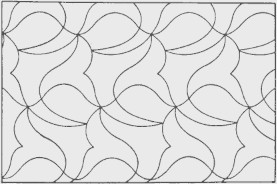
\includegraphics[scale=1.3]{./05_sensible/016}

Fig. 16. — La perception des « formes ».

{\it Que voyez-vous dans ce dessin de tapisserie ?}
\end{center}

Il est remarquable qu'aucune d’entre elles n’a indiqué l’espèce de sinusoïde
qui est cependant la « forme » la plus simple du dessin. Presque toutes y
ont vu « des fleurs » mêlées à des dessins de fantaisie. Un enfant de cinq ans
y a aperçu « des queues de poisson ». Un adulte y a discerné « des sortes de
crocs ou d’enclumes de cordonnier ». Il est évident que des {\it schèmes} perceptifs
dus à l'expérience antérieure viennent s’interposer ici entre le donné
sensible et l'interprétation perceptive.}
\vspace{0.31cm}

\section{Du syncrétisme aux objets distincts}% 83.
{\it A.} Ce qu’on peut
retenir de la théorie de la Forme, c’est que la perception ne part pas,
chez l’enfant, d'éléments isolés, mais de certains {\it ensembles} et que ces
ensembles {\it ne sont pas}, primitivement, des ensembles {\it analysés} ni des
ensembles {\it construits} : ils sont perçus \textbf{\textit {syncrétiquement.}}

\vspace{0.24cm}
{\footnotesize 
Quelques exemples feront mieux comprendre en quoi consiste ce syncrétisme.
Claparède cite le cas d’un enfant de 4 ans à qui l’on avait appris
les {\it Rondes enfantines} de Dalcroze, sa mère l’accompagnant au piano.
Quelques semaines après le début de l'apprentissage, l'enfant sait ouvrir
l’album à la page voulue pour demander qu'on lui joue telle ronde déterminée.
%103
Nous avons constaté nous-même qu’un enfant de 4 ans sait parfaitement
distinguer, parmi un assez grand nombre d’autres, un disque de
phonographe à son étiquette. Voici enfin un cas particulièrement typique :
on montre à un enfant de 5 ans quarante et une images représentant les
facteurs de pays différents, avec, dans les coins, un timbre-poste et le
drapeau du pays correspondant ; l’enfant apprend très vite les noms des
41 pays. Après une interruption de trois mois, il sait les dire encore pour
13 images. On lui demande à quoi il les reconnaît. Il déclare tantôt que
c’est grâce au timbre, tantôt que c’est grâce au drapeau, tantôt enfin au
képi du facteur. Or {\it il reconnaît encore les images quand ces détails sont
cachés}. En réalité, un syncrétisme s’est établi entre les noms de pays qu’on
lui a appris et «la physionomie générale de l’image »
{\scriptsize (Il est à remarquer que cet exemple de T. Jonckheere, comme celui de Claparède,
est cité dans les {\it Archives de psychologie} de 1908, donc bien avant le développement des
théories gestaltistes)}.}
\vspace{0.31cm}

Ce syncrétisme n’est pas, à proprement parler, une perception
structurée, organisée, comme le voudrait le Gestaltisme. L’enfant ne
prend pas conscience des rapports. Il est, commentait Claparède,
« dans le même état d’esprit qu’un adulte qui ignore et qui ne sait pas
qu’il ignore. Il n'analyse pas ce qu’il a sous les yeux, si les parties
du tout qu'il observe lui sont encore inconnues ou ne suscitent pas
son intérêt d'une façon particulière ». C’est à peu près dans le même
sens que H. Piéron a dit que, dans un jardin ensoleillé où dort un
chien, ce que le tout jeune enfant perçoit d’abord, c’est l’ensemble :
{\it le jardin-au-soleil-avec-le-chien}. « De cet ensemble, le jardin, le
chien et le soleil se dissocieront comme réalités indépendantes,
puis l’aboiement, la toison du chien s’individualiseront. » Comment
va s’opérer cette dissociation ? Comment vont se dégager les objets
perçus ?

{\it B.} Remarquons d'abord que la loi du syncrétisme ne vaut pas
{\it également} pour tous les sens. Ainsi que le note J. DeLay, les Gestaltistes
« n'ont guère étudié les lois du complexe de la Forme que dans
le domaine optique. Or il y a une différence fondamentale entre les
“ formes ” optiques et les “ formes ” tactiles. Dans le domaine visuel,
la perception du tout est aussi immédiate que la perception des
parties et même elle la précède. Dans le domaine \textbf{\textit {tactile,}} le complexe
ne naît que par synthèse active des formes élémentaires et partielles ».

{\it C.} Chez l’homme, le toucher présente d’ailleurs une importance
toute particulière du fait qu’il est l’organe principal de l’\textbf{\textit {action}} sur
le monde extérieur, et l’on ne saurait trop insister à ce propos sur le rôle
de la {\it main} dans la représentation que nous nous faisons des objets :
les animaux qui ne disposent pas d’une main préhensive ne perçoivent
%104
pas les choses comme nous. Mais il y a lieu de généraliser :
« {\it Reconnaître un objet usuel}, a dit Bergson, {\it consiste surtout à savoir
s’en servir}. » La perception a d’abord une fonction pratique : son
rôle est de « préparer des actions » ; elle est « la mesure de notre
action possible sur les corps » ; et elle ne retient du réel que ce qui est
utile à notre action présente. « Le monde est peut-être, dit encore
Bergson, une continuité indistincte. Chaque êtke découpe le monde
selon les lignes mêmes que son action doit suivre. » On a vu (\S 40)
que l’enfant définit d’abord les objets par l’{\it usage}. Mais nous-mêmes
que percevons-nous d’abord dans un crayon ou un stylo, sinon l’objet
qui sert à écrire ? dans un couteau, sinon l’objet qui sert à couper ?
dans une chaise ou un fauteuil, sinon l’objet qui sert à s’asseoir ?
N'est-ce pas ce rapport avec notre {\it action} qui fait pour nous l’unité de
l’objet, beaucoup plus que sa « forme » au sens gestaltiste ?

{\it D.} Plus généralement encore, il faut invoquer ici \textbf{\textit {l’intérêt affectif,}}
lui-même en relation avec nos {\it besoins} et nos {\it tendances}. « L'unité de
l’objet est déterminée par un acte particulier qui dépend des besoins
et des tendances de l’organisme. C’est le besoin de boire qui donne
naissance à l’objet que nous appelons de l’eau. C’est le besoin de
manger et la tendance à manger qui donne de l’unité au fruit. Ce qui
établit l’unité et la physionomie d’une chose, c’est la satisfaction ou
l’insatisfaction directe ou indirecte de nos tendances » (Janet). Chez
le nouveau-né, c’est l'intérêt qui, du syncrétisme primitif, fait surgir
quelques ensembles individualisés : la maman ou la nourrice, le
biberon, etc. Autrement dit, il y a, selon l’expression de Piaget,
« assimilation des choses aux {\it schèmes} (héréditaires ou acquis) du sujet » :
ces schèmes sont par exemple ceux de la succion, de la vision, de la
préhension. Mais, à ce stade, l’univers consiste beaucoup moins en
objets permanents qu’« en tableaux perceptifs mobiles et plastiques,
centrés sur l’activité propre » (voir \S 102).

\vspace{0.24cm}
{\footnotesize 
Cette structure mentale égocentrique du tout jeune enfant se traduit
encore plus tard dans ses {\it dessins}. G. Luquet avait déjà montré que, chez
l’enfant, « l'intention de dessiner tel objet n’est que le prolongement et la
manifestation de sa représentation mentale ». L'enfant dessine, non ce qu’il
a sous les yeux, mais un {\it type} : le bonhomme, la maison, etc., qui « correspond
à une réalité psychique existant dans son esprit », et qui constitue un
véritable {\it modèle mental}. Autrement dit, il dessine {\it ce qu’il sait}, non ce qu'il
voit : ainsi, dans une sonnette à main posée sur une table, il dessine le
battant, quoique celui-ci ne soit pas visible, parce qu'il {\it sait} qu'il existe
(fig. 17). Une étude plus récente de M. Prudhommeau (sur {\it Le dessin de
l'enfant}) a confirmé ce résultat ; mais elle a montré en même temps combien
est complexe le passage de ce réalisme intellectuel au réalisme visuel.
Les premiers dessins de l'enfant relèvent uniquement du réalisme intellectuel : 
our figurer « un bonhomme », il commence par dessiner le classique
%105
« bonhomme tétard » qui est « {\it la projection de l’image qu'il se fait de son
corps} », {\it des postures qu’il parvient à dominer lui-même} dans son équilibre
interne et externe. Le réalisme visuel qui apparaît vers 8-9 ans implique au
contraire la prise de conscience {\it objective} des rapports posturaux corrects.

\begin{center}

\includegraphics[scale=0.9]{./05_sensible/017}

Fig. 17. — Le dessin enfantin.

(D’après Luquet, {\it Les dessins d'un enfant},

et Prudhommeau, {\it Le dessin de l'enfant}, P. U. F., éd.).
\end{center}

A et B. {\it Bonshommes tétards dessinés par des enfants de 3 ans 1/2 : l'enfant dessine d’abord
une tête à laquelle sont directement attachés les bras (quand il les dessine) et les jambes.
Mais cetle tête symbolise, en réalité, pour lui « l'ensemble du corps humain »} (Prudhommeau).
— {\it C'est ce que montre bien le dessin C (enfant de 4 ans, 1 mois) où les bras sont
attachés aux jambes, avec un trait horizontal qui est peut-être déjà une ébauche de figuration
du tronc. Ce n'est que vers 5 ans que celui-ci apparaît de façon distincte}. — D. {\it Dessin
d'une sonnette par un enfant de 7 ans 4 mois}.}
\vspace{0.31cm}

\section{La construction des objets}% 84.
Il importe d'ajouter que,
dans la constitution des objets, il intervient ainsi un processus de
{\it construction} (et non seulement de dissociation), fonction de l’expérience
acquise, ce que la théorie gestaltiste risquerait de nous faire
méconnaître. Un objet est un complexus de propriétés qui, le plus
souvent, intéressent {\it différents sens}. Or il n’y a pas {\it a priori} de liaison
nécessaire — quoique, pour l’enfant, il y ait souvent un lien syncrétique,
mais arbitraire
{\scriptsize (Un enfant dira volontiers que « les gâteaux roses » ou « les bonbons rouges », c'est
bon. — Nous avons fait l'observation suivante sur un enfant d'environ cinq mois.
Alors qu’il commence à faire jour, un réveille-matin, tout à côté duquel se trouve une
veilleuse encore allumée, se met à sonner. L'enfant, déjà éveillé, regarde avec un étonnement
évident, non le réveil, mais la veilleuse, quoique de son berceau il puisse voir
les deux)}
 — entre ces différentes qualités sensibles :
entre la couleur et la saveur par exemple. Nous avons, de l’univers
qui nous entoure, un « atlas tactile » et un « atlas visuel », comme
disait Taine, et les observations faites sur les aveugles-nés opérés et
devenus voyants montrent qu’ils se trouvent parfois tout à fait
dépaysés dans ce monde visuel nouveau pour eux et qui n’a pas, en
principe, de commune mesure avec le monde tactile auquel ils sont
habitués : on a souvent cité l’exemple du jeune aveugle opéré par le
%106
chirurgien anglais Cheselden (1728) qui ne pouvait distinguer le chat
et le chien de la maison, qu’il connaissait bien par le toucher, jusqu’au
jour où il les caressa et regarda en même temps. La jonction de ces
différents « atlas » se fait peu à peu par l’expérience et souvent l'{\it expérience
active} (chez l’enfant, à partir de l’âge de 4-5 mois, palpation,
manipulation des objets, en même temps qu'il les regarde, les écoute
s’ils font du bruit, etc.). On verra plus loin que cette {\it construction} peut
se poursuivre jusque chez l’adulte sous la forme de ce qu’on appelle
les « perceptions acquises » (\S 87 B).

\section{Les cadres sociaux de la perception}% 85.
L'homme, rappelons-le
(\S 24 et 32), est un {\it être social}, et le monde qu’il se construit,
est fonction non seulement de l’être vital, mais aussi de l être social
qui est en lui. L. Lévy-Bruhl a pu écrire que « les primitifs ne perçoivent
rien comme nous », non que leurs sens ou leur appareil cérébral
soient différents des nôtres, mais parce que des \textbf{\textit {représentations
collectives}} différentes des nôtres viennent se mêler chez eux à la
perception ou plutôt en sont « partie intégrante ». Quel que soit
l'objet qui se présente à eux, il implique des propriétés « mystiques »,
comme dit Lévy-Bruhl, disons plutôt : magiques. Pour eux, « il
n’y a pas de fait proprement physique, au sens que nous donnons à
ce mot » : tout ce qu’ils perçoivent, l'eau qui coule, le vent qui souffle,
la pluie qui tombe, un son, une couleur, implique des « participations »
mystérieuses, des propriétés invisibles. Comme le remarquait
Ch. Blondel, « entre les primitifs et nous, l'humanité a passé par
toute une série de visions collectives du monde où la conception de
la réalité s’est graduellement dépouillée de ce caractère mystique
pour se faire de plus en plus positive ». — En fait, ainsi que le remarquait
récemment L. Goldmann (à propos de la peinture de Chagall)
« tout groupe social, orienté vers une organisation globale de la société,
tend à élaborer une vision cohérente [c’est-à-dire universelle] du
monde qui, étant donné que les innombrables distorsions individuelles
s’annulent les unes les autres, est mieux réalisée et, par cela, plus facile
à saisir dans le groupe que chez la plupart de ses membres pris individuellement. »

Blondel observait encore que le monde dans lequel vit l’homme
moderne n’est pas fait d'objets naturels, mais d'\textbf{\textit {objets fabriqués,}}
produits d’une certaine technique. Or « l'interprétation de la plupart
d’entre ces objets implique une initiation sociale. Quand nous
disons : voici un chapelet ou voici un appareil téléphonique, notre
affirmation dépasse énormément la simple constatation des formes
en effet perçues, elle suppose une connaissance de techniques religieuses
%107
ou scientifiques que nous devons uniquement à notre milieu ».

À plus forte raison en est-il ainsi des \textbf{\textit {symboles}} ou des \textbf{\textit {emblèmes.}}
« Au premier coup d'œil, nous percevons quelle profession ou quel
commerce s’exercent dans les boutiques ou les maisons des rues que
nous parcourons, à des particularités d’ornementation ou de disposition
qui, variables en général d’un pays à l’autre, sont toutes
conventionnelles et symboliques, tels en France l’écusson des notaires,
la carotte des bureaux de tabac ou [jadis] le plat à barbe des coiffeurs »
(Blondel). Qu'on songe au nombre de conventions qu’implique un
simple {\it signal}, comme les signaux qui règlent la circulation dans les
rues d’une ville et, bien plus encore, à l’ensemble de {\it croyances}, de {\it sentiments},
de {\it traditions} que représente un emblème, tel que le drapeau,
la croix ou le croissant !

Ajoutons que la perception de l’objet est liée pour nous à son
\textbf{\textit {nom,}} à tel point qu’on pourrait dire : « {\it Reconnaître un objet consiste à
savoir le nommer}. » L'enfant, comme le remarque E. Cassirer, a
une véritable « faim de noms », mais ce n’est pas que son intérêt
s'attache « à l’acte de désignation, que d’ailleurs il ignore encore
complètement en tant qu’acte isolé ». Il demande le nom « pour prendre
en quelque sorte par lui possession de la conscience de la chose: il se
produit entre la chose et le nom une véritable {\it concrescence} ». Pour lui
comme pour le primitif, « le mot est un élément objectif de la chose
et constitue son essence propre ». Même chez nous, le nom donné à
l’objet réagit sur la représentation que nous nous en faisons. Plus
généralement, le nom de l’objet « l’attire avec lui dans ce monde de
relâtions logiques qu’est précisément le monde de nos mots » ; car,
étant généralement un nom commun, il « affirme à la fois qu’outre
ses céractères individuels l’objet nommé en possède d’autres qui
l’apparentent aux objets de la même espèce et que, faisant partie
d’une espèce, il se situe à une place définie dans l’ensemble de notre
expérience et des notions où elle trouve son unité » (Blondel).
Autrement dit, nommer un objet, c’est le {\it classer}, c’est-à-dire l'intégrer
à toute une représentation du monde cristallisée dans le {\it langage}.

Il faut tenir compte enfin des dispositions mentales créées par la
\textbf{\textit {situation sociale}} du sujet. « L'agent de police, l’assistante sociale, le
politicien de clocher, le touriste étranger qui se promènent dans le
même quartier de taudis, non seulement interprètent différemment
ce qu’ils voient, mais encore perçoivent vraiment des choses différentes »
(Krech et Crutchfield).

\section{La perception individualisée}% 86.
Les facteurs de dissociation
et de construction examinés jusqu'ici ne nous donnent encore
%108
qu’une perception {\it générique} des objets : l’usage pratique ou social
caractérise toute une {\it classe} d'objets, et le nom, remarquions-nous,
est {\it commun}. Comment parviendrons-nous de là à la perception \textbf{\textit {individualisée,
singulière ?}}

« Il y a perception singulière des êtres concrets, personnes ou choses,
lorsque notre perception nous apporte la connaissance non de l'espèce
à laquelle son objet appartient, mais celle de cet objet lui-même, discerné
comme tel de tous les objets du même genre » (Blondel). Or
certains malades (syndrome dit de Korsakoff) sont capables d’identifier
les données de leurs perceptions, mais non plus de les individualiser :
« Ils savent qu’ils sont dans un hôpital, mais, d’un jour à
l’autre, d’un instant à l’autre, ils sont hors d’état de reconnaître
qu’ils sont dans le même hôpital. Ils savent qu’ils parlent à un
médecin, mais, si répétées qu’aient été leurs rencontres avec lui, il
demeure toujours pour eux un nouveau venu. » L'étude des dessins
d’enfants montre que c’est seulement à partir d’un certain âge qu’apparaissent
« les dessins figurant des motifs individuels nettement spécialisés
par leurs détails distinctifs » ; que l’enfant dessine par exemple
non plus {\it la} maison en général, mais {\it une} maison qu'il a devant lui.
Tout ceci prouve que la perception personnelle et, comme dit Blondel,
« historique » — car elle implique la conscience de notre « histoire »,
du passé propre à chacun de nous — est une opération relativement
indépendante et qui met en jeu des fonctions élevées. Ce qui vient
d’être dit montre qu’elle suppose la \textbf{\textit {mémoire}} : il suffit parfois que
nous revoyions un livre, un paysage, une photo pour que toute une
scène de notre vie passée revienne à notre esprit. Elle suppose aussi
l'\textbf{\textit {attention}} : la reconnaissance d’un objet n’est possible qu’à l’aide
de ces {\it préperceptions} dont il a été question au \S 49 D. Elle suppose
enfin le \textbf{\textit {jugement.}} À vrai dire, pour les objets familiers, ce jugement
demeure le plus souvent implicite : il est à rapprocher de ces « jugements
naturels » qui, selon Malebranche, se font « en nous sans nous
et même malgré nous » et qui produisent des « sensations composées ».
Dans certains cas cependant, lorsque nous hésitons à identifier ce
que nous voyons de loin, ce que nous entendons sourdement, ce que
nous touchons dans une pièce obscure où nous nous déplaçons à
tâtons, nous prenons mieux conscience de l’{\it assertion} impliquée dans
la perception. Ainsi, nous voyons un point blanc sur la mer : nous
{\it jugeons} que c’est un bateau à voile ; nous entendons un crépitement
sur la vitre : nous {\it jugeons} qu’il pleut, ete. — La perception nous
apparaît ainsi comme étant déjà un véritable \textbf{\textit {acte intellectuel}}
({\it Exercice} 7).

%109
\section{« L'éducation des sens »}% 87.
Si la perception est, en partie,
construite, il en résulte que notre faculté de perception peut être,
dans une certaine mesure, éduquée. Il est cependant nécessaire de
distinguer ici comme deux plans différents.

{\it A.} Sur le plan de la \textbf{\textit {sensation}} proprement dite, une certaine éducation
est déjà possible par laquelle nos sens peuvent être {\it affinés},
acquérir une {\it acuité} (\S 78) supérieure. On dit que l’ouvrier des Gobelins
parvient à discerner plus de deux mille nuances différentes de vert :
ceci est évidemment acquis, non inné. Il y a lieu d’insister de nouveau
ici sur le rôle de l’{\it attention} dans une telle éducation : bien des gens se
plaignent d’avoir une mauvaise mémoire des couleurs, qui n’ont
jamais regardé attentivement la nature
{\scriptsize (C'est peut-être là ce qui fait la différence entre la perception chez l’homme et la
perception chez la femme. G. Heymans dit, dans sa {\it Psychologie des femmes}, que la
femme donne l'impression de percevoir plus finement que l’homme, alors qu’à l'examen
c'est plutôt le contraire qui apparaît comme vrai. La solution, ajoute-t-il, est dans cette
réflexion de Mme de Rémusat : « Apercevoir nous va mieux qu’observer. » La perception
spontanée est effectivement plus fine, mais c'est l'attention qui manque)}.
L’attention sensorielle
(\S 48) fait au contraire apercevoir dans un objet quantité de détails
ou d’aspects que nous n’y aurions jamais remarqués sans elle. C’est
grâce à elle que l’artiste se libère des perceptions clichées, stéréo-typées,
tout utilitaires, du sens commun pour {\it individualiser} sa vision
du monde et retrouver ainsi la sensation première dans toute son
originalité et sa fraîcheur (voir {\it Exercice} 6).

B. Mais l’éducation dite « des sens » est surtout, au vrai, une éducation
{\it de la perception}, qui consiste à enrichir la {\it signification} des
données d’un sens {\it de qualités relevant d’autres sens} ou même d’enseignements
plus généraux : ce sont les \textbf{\textit {perceptions acquises.}}

\vspace{0.24cm}
{\footnotesize 
Nous apprenons à juger à la couleur ou à l’odeur d’un fruit s’il est mûr ou
non, au toucher d’une étoffe si elle est en laine ou en coton, au son d’un
récipient s’il est vide ou plein, etc. « Tel distinguera à leur saveur la moitié
supérieure et la moitié inférieure d’une bouteille de vieux madère. Tel autre,
rien qu’à plonger sa main dans de la farine, vous dira si elle vient du Iowa
ou de Tennessee. Laura Bridgman, la sourde-muette-aveugle, avait le toucher
assez fin pour reconnaître à un an d'intervalle la main d’une personne
qui lui avait donné une poignée de main » (James). Un personnage de
Giraudoux reconnait, la nuit, au pas d’un paysan, de quel village il est, et
Marcel Proust, en s’éveillant, sait, aux bruits de la rue, quel temps il fait
({\it Exercice} 9). C'est ainsi encore qu’à la couleur d’un précipité le chimiste
détermine la nature d’un corps ; le médecin se sert de la palpation et de
l’auscultation pour apprécier l'état des organes ; au timbre de voix d’un
interlocuteur, nous discernons s’il est ému ou calme; etc.}
\vspace{0.31cm}

À vrai dire, « l’éducation des sens » se confond ici avec le développement
intellectuel : « Savoir regarder, dit P.-M. Schuhl, c’est tout
%110
le secret de l’invention scientifique, du diagnostic-éclair des grands
cliniciens, du “ coup d'œil ” des vrais stratèges. »

\section{Les erreurs de la perception}% 88.
La perception, étant une
opération complexe et, en partie, intellectuelle, est susceptible d’erreurs.
C’est ce qu’on a appelé les {\it erreurs des sens}, mais l’expression
est impropre : « Ce ne sont pas nos sens qui nous trompent, dit
Malebranche, mais c'est notre volonté qui nous trompe par ses
jugements précipités. » Il se glisse toujours en effet dans ces erreurs un
minimum d'\textbf{\textit {interprétation,}} donc, comme le dit Malebranche, de
\textbf{\textit {jugement,}} ne serait-ce que ce jugement erroné (\S 79) que nos sensations
sont les copies ou les images des réalités extérieures. — On peut
distinguer deux cas : tantôt l’erreur porte sur {\it un des caractères} de
l’objet, tantôt elle porte sur son {\it identité} même.

{\it A.} Dans le premier cas, l’erreur peut porter : sur la {\it forme} spatiale
de l’objet (cas du bâton à demi plongé dans l’eau et que l’on « voit »
brisé), sur sa {\it couleur} (phénomènes de contraste signalés au \S 73 C),
sur le {\it nombre} des objets perçus (expérience dite d’Aristote : si l’on
fait rouler une bille entre l'index et le médius préalablement croisés,
on sent deux billes au lieu d’une), sur leur {\it poids} relatif (illusion de
Demoor : de deux poids égaux, celui qui a le plus petit volume paraît
le plus lourd, même si les deux poids sont soupesés à l’aide d’anneaux
identiques), etc. Dans tous ces cas, il n’est pas difficile de découvrir
{\it un jugement implicite} : nous jugeons de la forme du bâton {\it comme
s’il était plongé dans un seul milieu réfringent}, l'air, ainsi qu’il arrive
en effet le plus souvent pour les objets que nous percevons ; dans
l'expérience d’Aristote, nous jugeons {\it comme si nos doigts étaient
dans leur position normale} ; l'illusion de Demoor n’existe ni chez le
tout jeune enfant ni chez le dégénéré : seul l’adulte normal se trompe
parce que, chez lui, l’appréciation ordinaire du rapport volume-poids
a fini par s’incorporer à la perception elle-même. — La plupart des
illusions d’optique s’expliquent ainsi par des phénomènes accessoires
provoquant des interprétations spontanées : un trompe-l’œil est toujours
un «trompe-l’esprit ».

\vspace{0.24cm}
{\footnotesize 
Dans la figure 18 A, c’est un phénomène d'{\it irradiation}, lequel fait que le
carré blanc empiète sur la rétine en dehors de sa propre zone, ce qui le fait
juger plus grand. Dans les figures 18 B et C, c’est l’action des {\it obliques},
qui provoquent des {\it mouvements} de l'œil brisant le parallélisme. Dans
18 D, ce sont les côtés des triangles semblables que l’œil a tendance à
suivre, ce qui déforme la circonférence. Enfin les figures 18 E et F donnent
des exemples des illusions de relief (\S 96).}
\vspace{0.31cm}
\begin{center}
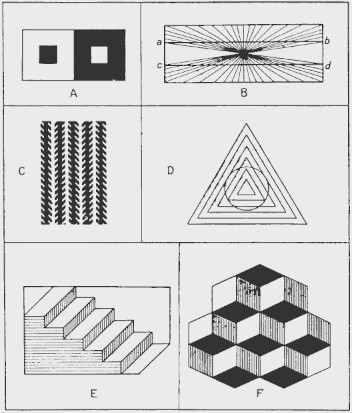
\includegraphics[scale=0.7]{./05_sensible/018}

Fig. 18. — Quelques illusions d'optique.
\end{center}
A. {\it Les petits carrés blanc et noir sont égaux}. — B. {\it Figure de Hering} : a b {\it et} c d {\it sont droites
et parallèles}. — C. {\it Figure de Zollner : les verticales coupées par des obliques sont parallèles}.
— D. {\it Figure de Gatti : cercle déformé par les triangles}. — E {\it et} F. {\it Illusions de
relief} (E, {\it escalier de Schrüder} ; F, {\it on voit tantôt 6, tantôt 7 cubes}).

%111
{\it }B. Dans le second cas, celui des illusions proprement dites, {\it nous prenons
un objet pour un autre, une personne pour une autre}. Ici l’interprétation
surajoutée aux données sensibles est évidente, d’autant
plus qu’elle est généralement en relation avec {\it un état global de la
conscience}. Si de loin nous prenons une personne quelconque pour

%112
un de nos amis, c’est bien souvent parce que nous attendons celui-ci.
Si le peureux voit, la nuit, dans les buissons ou les arbres de la route,
des fantômes ou des brigands, c’est précisément parce qu’il est peureux.
Un passant voit, à ‘la devanture d’un libraire, des livres traitant
de sciences occultes et, à côté, des livres d'histoire parmi lesquels
1815 de Henri Houssaye ; au lieu de 1815, il lit ISIS (les mystères
d’Isis sont connus des occultistes). Regardant par la fenêtre, Edgar
Poë croit voir un animal gigantesque marcher sur la crête d’une colline
qui se profile à l’horizon (au lieu d’un moucheron qui se promène
sur la vitre). Mais son amour du fantastique n’y est-il pour rien?

(Phot. Bibl. Nat.)

\begin{center}
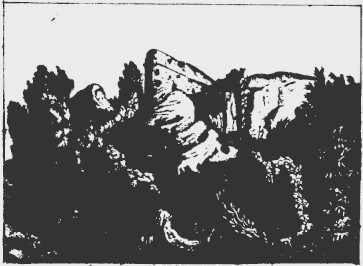
\includegraphics[scale=0.7]{./05_sensible/019}

Fig. 19. — Une estampe amusante.
\end{center}

{\it Au {\footnotesize XVIII}$^\text{e}$ siècle s'était répandue la vogue des « estampes amusantes », notamment de celles
qui présentent un double sens. La gravure ci-dessus prétend représenter le château de
la ville de Pépa, comitat de Veszprem, en Hongrie. Mais, si on la place sur le côté gauche,
dans le sens de la hauteur, elle apparaît tout autrement.}

%113
On trouvera de nombreux exemples de ces illusions dans les œuvres de
Marcel Proust. Tantôt, au bord de la mer, il aperçoit au loin une ligne
blanche qu'il prend pour une chaussée de pierres ou une digue : c’est seulement
lorsqu'il voit un navire s’y aventurer qu'il comprend que c’est une
frange d'écume. Tantôt, le matin au réveil, apercevant une lueur allongée
à un certain endroit de sa chambre, il croit que c’est le jour qui commence à
filtrer sous les rideaux de la fenêtre : c'est une tringle de cuivre devant la
cheminée, où se reflète une dernière braise du foyer. L'idée qu’il doit commencer
à faire jour est ici à la base de l'erreur.

Un phénomène analogue se produit dans les images à sens multiples
ou les images-devinettes, telles que celles des figures 8, 17 {\it E} et {\it F}
et 19 : il est très remarquable qu’à un moment donné c’est {\it une}
interprétation qui s'impose ; le passage à {\it une autre} interprétation
se fait brusquement. Il y a bien ici, sinon tout à fait une « forme »
au sens gestaltiste, du moins un « modèle mental », une orientation
de l'esprit à la base de l'interprétation.

\section{Sujets de travaux}% SUJETS DE TRAVAUX

{\bf Exercices.} — 1. {\it Analyser introspectivement la sensation kinésique en
distinguant} : a. {\it la sensation} musculaire ({\it par exemple, quand on contracte le
biceps en laissant l'avant-bras immobile}) ; b. {\it la sensation} tendineuse ({\it en
crispant la main comme pour griffer quelqu'un}) ; c. {\it la sensation} articulaire
({\it en faisant tourner la main autour du poignet, le coude étant posé sur une
table}). — 2. {\it Observez le phénomène de la} vision crépusculaire. — 3. {\it Expliquez
et commentez ce texte d'A. Gide :} « La vue — le plus désolant de nos sens.
Tout ce que nous ne pouvons pas toucher nous désole ; l'esprit saisit plus
aisément la pensée que notre main ce que notre œil convoite. » — 4. {\it Commenter
cette phrase de Van Gogh :} « Cette combinaison d'ocre rouge, de
vert attristé de gris, de traits noirs qui cernent les couleurs, cela produit
un peu la sensation d'angoisse dont souffrent souvent certains de mes
compagnons d'infortune et qu'on appelle {\it noir-rouge}. » — 5. {\it Comment
comprenez-vous ce mot de Ruskin} : « L’essence de la vulgarité réside dans
l'absence de sensations » ? — 6. {\it Commentez cette citation d’Eugène Delacroix :}
« La loi du vert pour le reflet et du bord d'ombre ou de l'ombre portée, que
j'ai découverte antérieurement dans le linge, s'étend à tout comme les
trois couleurs mixtes [orangé, vert, violet] se retrouvent dans tout... Sur
la mer, c’est aussi évident. Les ombres portées évidemment violettes,
et les reflets toujours verts, aussi évidemment. » — 7. {\it Expliquez ce jugement
d'Alain :} « La perception est déjà une fonction d’entendement..., l'esprit
le plus raisonnable y met de lui-même bien plus qu'il ne croit. » — 8. {\it Commentez
ce texte de Marcel Proust :} « Dès le matin, la tête encore tournée contre
le mur, je savais déjà le temps qu'il faisait. Les premiers bruits de la rue
me l'avaient appris selon qu’ils me parvenaient amortis et déviés par
l'humidité ou. vibrants comme des flèches dans l'aire résonnante et vide
d'un matin spacieux, glacial et pur ; dès le roulement du premier tramway,
j'avais entendu s’il était morfondu dans la pluie ou en partance pour
l'azur. » — 9. {\it Cherchez et analysez quelques exemples d'illusions sensorielles
(auditives notamment) analogues à celles du \S 88 A.}

%114

{\bf Exposés oraux.} — 1. {\it Le caractère purement qualitatif de la sensation et la
critique de la Psychophysique}, d’après Bergson, chap. I. {\it Discussion} (voir
Pradines, p. 417-453). — 2. {\it La théorie de la Forme, appliquée à la perception,}
d’après GuiLLaume.

{\bf Discussions.} — 1. {\it La distinction entre} sensation {\it et} perception {\it a-t-elle
perdu toute valeur ?} — 2. {\it Discuter ce passage de J.-P. Sartre :} « Certains
rouges de Matisse provoquent une jouissance sensuelle chez celui qui
les voit. Mais cette jouissance, si on la considère isolément — par exemple,
si elle est provoquée par un rouge donné en fait dans la nature — n’a rien
d'esthétique. C’est purement et simplement un plaisir des sens. Lorsqu'on
saisit, au contraire, le rouge sur le tableau, on le saisit malgré tout comme
faisant partie d’un ensemble irréel et c’est dans cet ensemble qu’il est beau. »

{\bf Lectures.} — {\it a.} Bergson, {\it Les Données immédiates de la conscience}, Alcan,
1888, chap. I. — {\it b.} Ch. Blondel, {\it Introd. à la psychologie collective}, coll.
A. Colin, 1928, 2$^\text{e}$ partie, chap. I. — {\it c.} M. Pradines, {\it Philosophie de la
sensation}, Belles-Lettres, 1928 ; et {\it d. Traité de Psychologie générale},
P. U. F., 1943, tome I, p. 399-470 et 497-538. — {\it e.} G. Dumas, {\it Nouveau
Traité de Psychologie}, Alcan, 1932-1936, tome II, liv. II, et tome V, p. 1-75
et 79-84 (B. Bourdon). — {\it f.} E. Cassirer, {\it Le langage et la construction du
monde des objets}, dans le {\it Journal de Psychologie}, année 1933, p. 18. —
{\it g.} P. Janet, {\it Les Débuts de l'intelligence}, Flammarion, 1935, 2$^\text{e}$ partie,
chap. V. — {\it h.} P. Guillaume, {\it La Psychologie de la forme}, Flammarion,
1937, chap. III. — {\it i.} P. Chauchard, {\it Les Messages de nos sens}, P. U. F.,
1944. — {\it j.} M. Merleau-Ponty, {\it Phénoménologie de la perception}, Gallimard,
1945. — {\it k.} H. Piéron, {\it La Sensation, guide de vie}, Gallimard, 1945.
— {\it l.} J. Piaget, {\it Psychologie de l'intelligence}, coll. A. Colin, 1947, chap. III. —
{\it m.} D. Krech et R. S. Crutchfield, {\it Théorie et problèmes de Psychologie
sociale}, P. U. F., 1952, chap. III et IV. — {\it n.} J. Piaget, {\it Les mécanismes
perceptifs}, P. U. F., 1961. — {\it o.} Paul Fraisse et J. Piaget, {\it Traité de Psychologie
expérimentale}, fasc. II : {\it Sensation et motricité}, par Pieron, Chocolle
et Leplat, et fasc. VI : {\it La Perception}, par Piaget, Fraisse, Vurpillot
et Francès, P. U. F., 1963. — {\it p.} Robert Francès, {\it La Perception}, P. U. F.,
1964. — {\it q.} H. Gratiot-Alphandéry et R. Zazzo, {\it Traité de psychologie de
l'enfant}, 3 vol., P. U. F., 1970.

%
\chapter{L'espace}
% chapitre VI
%L'ESPACE
%89. La perception de l'étendue : différents problèmes. — 90. Le problème
%psychologique. — 91. « L'espace perceptif ». — 92. La construction de
%l'espace. — 93. Espace, mouvement et réalité. — 94. La perception de
%la troisième dimension. — 95. L'appréciation de la distance. — 96. Erreurs
%et troubles de la perception de l’espace. — 97. Le concept d'espace. — 98.
%Le problème épistémologique. — 99- Le problème métaphysique.

\section{La perception de l'étendue : différents problèmes}% 89.
La perception sensible présente encore un autre caractère, — d'ailleurs
difficilement isolable, on le verra bientôt, de celui que nous étudierons
dans le chapitre suivant : le caractère \textbf{\textit {spatial.}} Les objets que nous
percevons nous paraissent {\it }étendus : ils présentent des plans, des
surfaces. Ils nous paraissent en outre se situer à une certaine {\it }distance,
offrir un certain {\it relief}, constituer des {\it volumes}. En un mot, nous percevons
les choses dans un {\it espace à trois dimensions}, comme douées de
longueur, largeur et profondeur. — Différents problèmes vont se
proposer ici à notre réflexion. Ce sera d’abord un problème psychologique :
ce caractère {\it spatial} est-il inhérent à la sensation, en tant
que donnée immédiate de la sensibilité ? ou bien est-il acquis, se forme-t-il
peu à peu ? Le problème \textbf{\textit {épistémologique}} consistera ici à s'interroger
sur la valeur et la portée de notre {\it idée}, de notre concept de l'espace,
question qui intéresse au premier chef la Géométrie, mais aussi toute
notre connaissance du monde extérieur. Le problème \textbf{\textit {ontologique}} ou
\textbf{\textit {métaphysique}} portera sur l’essence ou la réalité absolue de l’espace.

\section{Le problème psychologique}% 90.
Le problème psychologique
paraît ici plus aisé à poser qu’à propos de la notion d'objet. On va
voir pourtant que sa position même soulève des difficultés analogues.
Parmi les doctrines classiques, deux s'étaient opposées sur ce point,
dont l’une, le \textbf{\textit {nativisme,}} soutenait que la spatialité est une {\it donnée
%116
immédiate} de la connaissance sensible, que les impressions sensorielles
font naître, sans aucune expérience antérieure du sujet, des sensations
d’étendue, de formes, de distance, de profondeur, etc.{\scriptsize (Le
{\it nativisme}, qui est à peu près le point de vue du sens commun, ne doit pas
être confondu avec l'{\it innéisme}. Il soutient en effet que l'étendue (concrète)
est donnée {\it dans} l'expérience sensible elle-même, tandis que l’{\it innéisme},
celui de Kant par exemple (voir \S 97) admet que l’espace abstrait est une
forme {\it a priori}, c'est-à-dire {\it antérieure}, au moins en droit, à toute expérience
possible)}, —
tandis que l’autre, la théorie génétique (improprement appelée parfois
{\it empiriste}), regardait la perception de l’étendue (et, à plus forte
raison, le concept, l’idée abstraite d’espace) comme progressivement
acquise au cours de toute une éducation. Cette seconde théorie partait
de l’idée que la sensation est en elle-même quelque chose de
purement subjectif, donc de qualitatif et qui, par suite, ne peut
avoir primitivement quoi que ce soit de spatial. Le problème, à peu
près insoluble, était alors d'expliquer comment avec du non-spatial
l'esprit peut construire du spatial. On s’en tirait en ramenant la notion
d’espace, soit à celle de {\it coexistence} (Spencer), soit à celle d’{\it hétérogénéité
qualitative} (théorie des signes locaux de Lotze et Wundt{\scriptsize (Une
sensation tactile, disait-on, présente toujours, outre l'élément commun, une
différence qualitative qui varie selon les points du corps touchés. Ce sont ces
{\it signes locaux} qui nous permettent de localiser la sensation. Mais, pour
localiser une sensation, ne faut-il pas déjà avoir la notion d'espace? D'autre
part, eette théorie ne tenait pas compte de la {\it mobilité} des organes : la main
se déplaçant, n'importe lequel de ses points peut être impressionné par
n'importe quel point de l’espace. Enfin elle n'expliquait pas
la perception de la {\it distance})}).
Mais cette réduction était injustifiée. En outre, le point de départ était
faux ; on verra(\S 101 B) que la subjectivité pure n’est pas une donnée,
mais, tout comme l’objectivité, le produit de toute une évolution
psychique. — Le point de vue {\it nativiste} semble donc plus proche de
la vérité. De fait, gestaltistes, phénoménologues, existentialistes
reviennent aujourd’hui à un point de vue fort analogue. Au fond, nous
avons déjà touché à ce problème de l’espace quand nous avons parlé
de la perception des « formes » : « Une forme géométrique n’est pas
seulement une qualité originale : c’est un système de relations entre
des points, lignes, surfaces qui le constituent » (Guillaume). Or on
sait que, selon le Gestaltisme, la perception de ces « formes » est
immédiate. — De même, M. Merleau-Ponty nous dit : « Il est
essentiel à l’espace d’être toujours “ déjà constitué ” et nous ne le
comprendrons jamais en nous retirant dans une perception sans monde.
Il ne faut pas se demander pourquoi l’existence est spatiale. L’expérience
perceptive nous montre au contraire que [les faits qui constituent
la spatialité] sont présupposés dans notre rencontre primordiale avec
l’être et que l'être est synonyme d’être situé. » La profondeur, en
%117
particulier, qui est « la plus existentielle de toutes les dimensions »,
est « vécue hors de toute géométrie ». En ce sens, « il n’y a pas de problème
de la distance ». Nous avions déjà remarqué, à propos de la
notion d’objet, que les théories de « l’expérience immédiate » tendent
à supprimer les problèmes.

Mais ici aussi il y a lieu de faire la part de ce qui est valable dans
cette conception et de ce qui ne peut être admis. Ce qui est vrai, c’est
que la perception de l’espace est inséparable de la perception des
choses et qu’il n’existe pas de « perception sans monde »; c’est aussi
que, dans la mesure où la perception s’objective, elle vient s’intégrer,
comme le dit J. Piaget, à « un système spatio-temporel et causal »
(cf. \S107) ; c’est enfin que ceci ne peut avoir lieu qu’à condition que,
— de même que la conscience est spontanément tournée vers l’objet,
— la perception présente dès l’origine quelque structuration d’où
l'espace ne soit pas absent. — Mais nous retrouvons ici une équivoque
exactement parallèle à celle que nous avons rencontrée dans les
mêmes théories à propos de la notion d’objet. Cette structuration de
« l’espace perceptif » est bien loin encore d’être celle de l’espace {\it représenté}
et, à plus forte raison, celle de l’espace {\it géométrique}, tel que
l'espace euclidien. La philosophie de « l'expérience immédiate » paraît
bien être ici dupe d’une illusion qu’on pourrait appeler l’{\it illusion de
l'immédiat} (ci-dessus, \S 58-59) : « L’adulte, ayant perdu tout souvenir
des étapes antérieures à une telle transformation, s’imagine alors que
chaque perception utilise dès l'origine les systèmes de coordonnées ou
les rapports de verticalité et d’horizontalité, en réalité très complexes,
qui sont achevés seulement entre 8 et 9 ans » (J. Piaget). Selon
Piaget, les faits correctement observés « démontrent au contraire de
la manière la plus nette combien il est illusoire d’attribuer au sujet
humain la connaissance innée ou psychologiquement précoce d’un
espace d’emblée structuré selon un système de coordonnées rectangulaires
à deux ou trois dimensions » et, par suite, « il est évident que
la perception de l’espace comporte une construction progressive et
n’est pas donnée toute faite dès les débuts de l’évolution mentale ».

\section{« L’espace perceptif »}% 91.
Pour mieux voir comment s’effectue
cette {\it construction} de l’espace, demandons-nous en quoi peut
consister « l’espace perceptif » primitif en le distinguant soigneusement
de l’espace représenté. Certes il existe bien pour le tout jeune
enfant un milieu structuré lié à son activité, mais celui-ci demeure
« entièrement centré sur son activité propre » : c’est, selon l’expression
de Piaget, un « {\it espace pratique et égocentrique} » qui est encore
bien loin de la représentation d’un milieu ordonné comprenant le
%118
sujet lui-même à titre d’élément. Le physicien Mach (1838-1916)
avait déjà remarqué autrefois qu’il existe un « espace physiologique »
lié à nos mouvements et où l’on pourrait, à la rigueur, distinguer
trois dimensions « pratiques » : l’{\it avant} et l'{\it arrière}, le {\it haut} et le {\it bas}, la
{\it droite} et la {\it gauche}. Mais ces dimensions n’ont primitivement qu’un
caractère tout \textbf{\textit {subjectif}} et même affectif : l'{\it avant}, c’est la direction
de la tendance, du désir, celle de l’élan animal de l’être qui fond sur
sa proie ; le {\it bas}, c’est la direction dans laquelle nous nous sentons
attirés par la pesanteur ; quant à la distinction de la {\it droite} et de la
{\it gauche}, on verra plus loin qu’elle n’est nullement immédiate et qu’elle
est peut-être d’origine {\it sociale} plutôt que physiologique. Dans le même
ordre d’idées, W. James avait fait observer que certaines de nos
sensations au moins, peut-être toutes, présentent un caractère de
\textbf{\textit {voluminosité}} ({\it voluminousness}) : « Les grondements du tonnerre ont un
autre volume de sonorité que le grincement d’un crayon sur une
ardoise. Quand on entre dans un bain chaud, on éprouve une sensation
autrement {\it épaisse} que si une épingle vous égratigne. Une légère
douleur névralgique au visage paraît moins profonde que la douleur
pesante d’un furoncle ou la souffrance massive d’un lumbago. » Enfin
on s’accorde à reconnaître que les sensations de la vue, peut-être
aussi celles du toucher, ont une certaine \textbf{\textit {extensivité}} ({\it extensity}) : la
perception de la couleur est inséparable (autrement que par abstraction)
de celle d’une certaine {\it étendue} colorée ; même un point brillant
se détache sur un {\it fond} sombre ; quant au toucher, il est bien vain de
se demander, avec Maine de Biran, ce qu’il nous donnerait si son
organe était réduit à « un ongle très aigu » : en fait, c’est toujours une
certaine {\it surface}, si petite soit-elle, de notre peau qui est intéressée.
Mais cette voluminosité et cette extensivité ne sont encore que des
\textbf{\textit {qualités}} qui font corps avec la sensation elle-même : elles sont encore
bien loin de se projeter sous la forme d’un « espace objectif » dans un
milieu intellectuellement structuré et comportant des figures nettement
déterminées.

\section{La construction de l’espace}% 92.
J. Piaget a cru pouvoir
distinguer, chez l’enfant, trois périodes de la constitution du
« champ spatial » correspondant aux six stades de la constitution de
l’objet (\S 103). Chez le nouveau-né, ce qui est donné, c’est simplement
le champ des réflexes et des premières habitudes, c’est aussi « la
perception de la lumière et l’accommodation propre à cette perception ».
Au point de départ, « {\it l’espace n’est donc nullement la perception
d’un contenant, mais bien celle des contenus, c’est-à-dire des corps
eux-mêmes} ». C’est pourquoi \textbf{\textit {« la notion d'espace ne se comprend
%119
qu’en fonction de la construction des objets »}} (Piaget). Dans la première
période, qui correspond aux deux premiers stades de cette
construction, l’espace consiste en « groupes » purement {\it pratiques}, en
ce sens qu’ils demeurent liés à l’action, et {\it hétérogènes}, en ce sens
qu’il n'existe encore aucun lien entre les divers espaces sensoriels, entre
l’{\it espace buccal} qui est, selon Stern {\scriptsize (L. William Stern,
psychologue allemand (1871-1938))}, le premier de ces schèmes constitutifs
de l’espace enfantin (succion), et l’{\it espace tactile} (préhension), ni
entre celui-ci et l’{\it espace visuel} (l'enfant ne sait pas encore saisir un objet
qu’il voit). On ne peut guère supposer non plus, dans cette première
période, une véritable notion de la distance. De ce point de vue, l’espace
entier est pour l’enfant « analogue à l’espace céleste de la perception
immédiate : une masse fluide sans profondeur (bien que l’œil s’accommode
aux diverses distances), parcourue par des images qui s’entrepénètrent
ou se détachent sans lois et se déforment ou se reforment
alternativement ». Par exemple, dans un objet appuyé contre une
paroi, un vêtement pendu à un porte-manteau, le bébé ne voit qu’une
tache qui ressort à peine sur le fond. Une seconde période comprend
les troisième et quatrième stades de l’évolution sensori-motrice. Elle
est caractérisée, d’abord par la {\it coordination de la vision et de la préhension}
(d’où la constitution de « groupes », encore relatifs cependant à
la perspective propre de l’enfant : il apprend à saisir, donc à localiser
les objets {\it par rapport à lui}), puis, au quatrième stade, par la {\it coordination
des actions entre elles} (d’où la constitution du « groupe des
opérations réversibles » : l’enfant devient capable de cacher et de
retrouver, ce qui est un progrès vers l’espace objectif, mais sans qu’il
ait encore une notion nette de la position relative des objets {\it entre eux}).
La troisième période (à partir de l’âge d’un an) est caractérisée au
contraire par l’apparition de cette notion et la constitution de ce
qu’on peut appeler « {\it l’espace expérimental} » : au cinquième stade,
tout ce qui est perçu s'organise dans un champ commun et l’enfant
prend conscience de ses propres déplacements qu’il situe ainsi par
rapport à ceux des objets ; au sixième, l’enfant parvient au « groupe
représentatif » où l’espace est constitué comme un milieu immobile,
dans lequel il se situe lui-même.

\section{Espace, mouvement et réalité}% 93.
On voit donc ce qu’on
peut retenir des théories de l'expérience immédiate : gestaltisme ou
phénoménologie, et ce en quoi elles sont insuffisantes. — {\it A.} Le
Gestaltisme a bien vu {\it l'union étroite de la perception spatiale et du
mouvement} : « Dans une telle doctrine, écrit P. Guillaume, la sensibilité
%120
et la motricité sont étroitement unies. C’est dans la structure
même de l’excitation perceptive et de l’excitation motrice qu’il faut
chercher l’explication de leurs rapports. » C'est bien ce que vient de
nous montrer l’analyse précédente : espace perceptif et espace représenté,
malgré le « décalage » qu’exige le passage de l’une à l’autre, ont
cependant, selon Piaget, « un facteur commun », et ce facteur commun
qui présente ainsi « une importance essentielle pour l’interprétation
de l'intuition spatiale », c’est la \textbf{\textit {motricité,}} source des opérations
supérieures, notamment par l'intermédiaire du {\it dessin} (voir
{\it Exercice} 2), aussi bien que des « perceptions spatiales les plus élémentaires ».
— Mais le Gestaltisme a entendu cette union dans le
sens d’une détermination du mouvement par la perception des formes.
L’intuition de l’espace géométrique apparaît ainsi comme devant
être essentiellement de nature {\it contemplative, imagée}. L’analyse génétique
de Piaget établit au contraire qu’elle est de nature \textbf{\textit {constructive;}}
car c’est {\it l'élément moteur qui dirige l'élément figuratif ou imagé, et
non l'inverse}. « L’image visuelle d’une forme plane ou d’un volume en
perspective, d’une projection ou d’une section, d’un rabattement, etc.,
englobe bien plus de mouvements du sujet qu’on ne le croit généralement
et se trouve être beaucoup plus l’image d’une action possible
relative à ces formes qu’une action visuelle simple, »

{\it B.} D’autre part, il est parfaitement juste de dire avec M. Merleau-Ponty
que « l’espace n’est pas le milieu dans lequel se disposent les
choses, mais le moyen par lequel la position des choses devient possible »,
qu’il doit donc être pensé « comme la puissance universelle
de leurs connexions ». Toute l’analyse précédente nous a montré que
la construction de l’espace est \textbf{\textit {solidaire de la constitution des choses,}}
et c’est aussi ce que démontrent les deux expériences célèbres de
Stratton et de Wertheimer.

\vspace{0.24cm}
{\footnotesize {\it Expérience de Stratton.} — On sait que l’image des objets
se peint, sur la
rétine, renversée comme dans un appareil photographique, ce qui ne nous
empêche pas de les voir en position normale {\scriptsize (On s’est posé
d'ailleurs à ce sujet un problème parfaitement vain, celui de savoir comment
l'esprit (ou le cerveau) « redresse » l’image rétinienne. Mais « l’image
rétinienne n’a pas d'existence psychologique propre et l'image mentale n’est
pas son simple décalque » (H. Wallon). L'erreur est ici de s’imaginer une sorte
d’« œil interne » (esprit ou cerveau ?) qui regarderait l’image rétinienne
inversée comme notre œil regarde les objets, ce qui est pure mythologie :
car l'image rétinienne n’est pas « perçue ». Bien mieux, on peut dire qu’à
proprement parler elle n’existe pas. La rétine est constituée par une
mosaïque discontinue de cellules nerveuses dont chacune transmet au cerveau
l’impression reçue. Si cette pluralité d’impressions est interprétée par nous
comme une image continue et orthoscopique des choses, n'est-ce pas, ainsi que
le suggère encore H. Wallon, « en raison de leur maniement » qui, lui, ignore
les lois optiques ?)}. « Si l’on fait porter à un sujet des lunettes qui
redressent les images rétiniennes, le paysage entier paraît
%121
d’abord {\it irréel} et renversé ; au second jour de l’expérience, la perception
normale commence de se rétablir, à ceci près que le sujet a le sentiment que
son propre corps est renversé. Au cours d’une seconde série d’expériences
qui dure huit jours, les objets apparaissent d’abord renversés, mais moins
irréels que la première fois. Le second jour, le paysage n’est plus renversé,
c’est le corps qui est senti en position anormale. Du troisième au septième
jour, le corps se redresse progressivement et paraît être enfin en position
normale, {\it surtout quand le sujet est actif...} Les objets extérieurs ont de plus
en plus l’aspect de la « réalité ». Dès le cinquième jour, les gestes qui se
laissaient d’abord tromper par le nouveau mode de vision, vont sans erreur
à leur but... A la fin de l’expérience, quand on retire les lunettes, les objets
paraissent non pas renversés, mais « bizarres » et les réactions motrices
sont inversées : le sujet tend la main droite quand il faudrait tendre la
gauche {\scriptsize (Les expériences de G. M. Stratton (1896) ont été reprises
par P.H. Ewert (vers 1925) qui a montré la possibilité du rétablissement de la
vision droite au bout de 14 jours, avec mise en évidence du rôle de la loi de
l'effet selon laquelle toute réponse est renforcée par le succès, affaiblie
au contraire ou éliminée par l'échec.)} » (Merleau-Ponty).

{\it Expérience de Wertheimer.} — De même, « si l’on s'arrange pour qu’un sujet
ne voie la chambre où il se trouve que par l'intermédiaire d’un miroir
qui la reflète en l’inclinant de 45° par rapport à la verticale, le sujet voit
d’abord la chambre “ oblique ”. Un homme qui s’y déplace semble marcher
incliné sur le côté. Un morceau de carton qui tombe le long du chambranle
paraît tomber selon une direction oblique. L'ensemble est “ étrange ”.
Après quelques minutes, un changement brusque intervient : les murs,
l’homme qui se déplace dans la pièce, la direction de chute du carton
deviennent verticaux » (Id.).}
\vspace{0.31cm}

La première de ces expériences nous montre que « renverser un
objet, c’est lui ôter sa signification » (comme il est manifeste quand on
regarde un visage humain à l’envers), et toutes deux, que le sentiment
de {\it réalité} et la perception de l’{\it espace} sont intimement liés : dès que
cette dernière est perturbée, les objets paraissent irréels, étranges,
bizarres. L'expérience de l’espace, c’est notre expérience vécue du
monde où nous existons. Ce n’est pas une raison toutefois pour faire
de notre représentation de l’espace quelque chose d’{\it inanalysable.}
Nous avons vu, au contraire, que notre représentation de l’espace
\textbf{\textit {se construit}} peu à peu, non certes à partir d’une perception totalement
a-spatiale comme l’avait admis l’ancienne théorie génétique
(\S 90), mais à partir d’une spatialité implicite et encore très imparfaitement
structurée (\S 91-92), exactement comme notre représentation
du réel se construit, non certes à partir d’une « perception
sans monde », mais, on le verra (\S 102-103), sans prise de conscience
de l’objet comme tel. Dans cette construction de l’espace, interviennent :
1° une intelligence \textbf{\textit {active,}} et 2° la \textbf{\textit {motricité}} de notre
corps. 1° M. Merleau-Ponty reconnaît que, « si les déformations
perspectives nous étaient expressément données, nous
%122
n’aurions pas à apprendre la perspective ». Et en effet l'observation
la plus simple nous montre que notre représentation de la perspective
est toute farcie de conventions
qui d’ailleurs ont varié au cours des siècles et dans les différentes
civilisations. 
%(fig. 20)
N'est-ce pas avouer que notre représentation
géométrique de l’espace n’est pas toute donnée dans la
perception et qu’il s’y superpose une activité propre de l’intelligence ?
2° Enfin il ne suffit pas, pour exclure toute synthèse
des éléments sensibles et des éléments moteurs, de remarquer
que, dans l’expérience de Wertheimer, la rectification s’effectue
d’elle-même « sans aucune exploration motrice ». Croit-on
que notre expérience motrice antérieure n’y soit pour rien ? De
même, si dans l’expérience de
Stratton le sujet se trouve d’abord désemparé, n’est-ce pas que toutes
les coordinations sensitivo-motrices auxquelles il est habitué, se
trouvent perturbées ? Nous allons précisément constater le rôle
capital de ces éléments moteurs dans la perception de la troisième
dimension.
%Fig 20. — Les conventions de la prespective.
%(D'après Maspzno, L'Archéologie égyptienne, Grund et Maguet, éd.)

\section{La perception de la troisième dimension}% 94.
Par « troisième
dimension », il faut entendre la {\it distance}, la {\it profondeur}, et aussi
le {\it relief} qui est la distance, par rapport à nos sens, des différentes
parties de l’objet perçu. Les mêmes difficultés se sont présentées ici
qu’à propos de la perception spatiale en général. On a souvent tenté
en effet d’expliquer la perception de la troisième dimension comme
si elle procédait des deux autres: on s’imaginait que « l’image rétinienne »
ou l’image perçue, primitivement sans distance ni profondeur,
est ensuite {\it projetée à distance} grâce à différents facteurs dont
il sera question plus loin. Or on va voir qu’il faut totalement renoncer
à cette position de la question : la troisième dimension fait partie
intégrante de notre expérience totale de l’espace. Mais ce n’est pas
%123
une raison pour déclarer qu’il « n’y a pas de problème de la distance »
et pour nier ici toute évolution {\it génétique} et toute {\it activité} propre de
l’esprit : si l’objet est d’emblée perçu à distance, la représentation
correcte de la distance est le fruit de tout un apprentissage. Ici encore
il faut, avec J. Piaget, distinguer entre « le comportement et la
conscience ». L'enfant « accommode ses yeux et ses mains à la distance »
bien avant de savoir se {\it représenter} la différence entre objet proche
et objet éloigné comme une différence objective de profondeur.

{\it A.} L'expérience du toucher \textbf{\textit {moteur}}, l'expérience \textbf{\textit {kinésique}} est
inséparable, nous l'avons déja remarqué (\S 91), de notre expérienee
d’un espace à trois dimensions.

\vspace{0.24cm}
{\footnotesize « Vers les couleurs vives, vers les objets aux contours arrêtés,
l'enfant
tend les bras. Non qu'il ait déjà le sens de la direction et de l'éloignement :
les mouvements de ses bras et de son torse continuent simplement a s'acorder
avec ceux de ses yeux » (Th. Ruyssen). On peut rappeler ici les observations
du psychologue américain J.-M. Baldwin (1861-1934) sur sa fille
âgée de 9 mois. Il avait disposé, à différentes distances de l'enfant, des
papiers de couleurs variées capables d'attirer son attention. En pareil cas,
« l'enfant tient compte avec une régularité absolue des objets qui sont,
comme on dit, {\it à bout de bras} : avec plus d’hésitation déjà, il s'intéresse
aux objets situés à une distance qu'il peut, avant de savoir marcher,
atteindre avec extension du bras et flexion du tronc. Au delà, les objets
lui sont indifférents, bien qu’il les voie. Leur recul est un peu pour lui ce
qu'est pour l’adulte celui des étoiles : un {\it au delà} pratiquement inaccessible
et inappréciable pour les sens » (cf. \S 92). \textsf{\textit {Le « monde en profondeur » est donc
tout simplement celui de l'expérience motrice.}} Il y a pour l'enfant — et ceci
restera encore vrai, en grande partie, pour l'adulte — un « espace proche »
et un « espace lointain » (Piaget), le premier étant « le domaine des objets
à saisir », le second celui où nos gestes ne se sont pas encore risqués et où
« les distances relatives demeurent indiscernables ». — Plus tard même, la
notion que se fait l’enfant des distances, est fonction de ses {\it déplacements} :
« À 4 ou 5 ans, n'ayant jamais voyagé, je ne pus malgré tous mes efforts,
quand on me décrivit comme infinie la mer où se jetait la rivière de ma ville
natale, me la représenter que comme une pièce d’eau carrée de 4 ou 5 mètres
de côté. Et pourtant la riviére était bien large d’une cinquantaine de
mètres (Ruyssen). Anatole France enfant avait « acquis la certitude
que la Chine était derrière l'Arc-de-Trigmphe », Même chez l’adulte, il est
facile de voir que la {\it représentation} de la distance varie avec le genre de vie :
le paysan qui n’est jamais sorti de son village, imagine la France avec
l'étendue d’un canton.

On a souvent remarqué que nous évaluons les \textsf{\textit {distances verticales}} beaucoup
plus inexactement encore que les distances horizontales : c'est que, dans le
premier cas, nous manquons d'expérience motrice (indépendamment d'autres
raisons qu’on verra plus loin). C’est déjà vrai de l'enfant :
« Preyer {\scriptsize (W. Preyer, psychologue allemand (1841-1897), auteur
d’un livre célèbre sur l'Âme de l'enfant, 1881, trad. fr. 1887.)},
par la fenêtre d’un second étage, lance un papier à un enfant de près de
%124
deux ans. Celui-ci ramasse l’objet et le lui tend avec le désir visible de
recommencer ce jeu. » Que de bévues ne commettons-nous pas nous-mêmes sur
l’appréciation de la hauteur d'un phare, d’une tour, d’un clocher et surtout
d’un avion dans le ciel ! Mais on avait déjà observé jadis que « les marins,
habitués à grimper dans les cordages, ont l'œil autrement juste », et aujourd’hui
l’aviation a ajouté à notre expérience de l’espace la dimension verticale.
— Il est à noter cependant que, dans cette expérience, il entre une
certaine \textsf{\textit {activité de l'intelligence}}. Un garçonnet de 7 ans observé par Franz
(vers 1840) et « qui n’avait aucun défaut de la vue, mais dont l'intelligence
était faible », était incapable d’estimer la distance verticale des objets :
« il tendait fréquemment la main vers un clou du plafond ou vers la lune ».}
\vspace{0.31cm}


{\it B.} La perception de la distance \textbf{\textit {par la vue}} a été l’objet de nombreuses
discussions. Certains auteurs ont prétendu que la vue ne
nous apporterait par elle-même {\it aucune expérience de la distance} et nous
fournirait seulement {\it des images sans relief}. Tout au plus, certains
éléments, surtout moteurs, du processus de la vision nous permettraient-ils
un {\it apprentissage progressif} de la vision à distance. Mais on
verra que les arguments de base sont {\it sans valeur} et que les éléments
en question ne pourraient nous donner cette perception à distance
{\it si nous ne la possédions déjà}.

\vspace{0.24cm}
{\footnotesize 1° Les arguments invoqués étaient : $\alpha$. {\it l'argument de Berkeley}
{\scriptsize (George Berkeley, évêque anglican et philosophe irlandais,
1685-1753. Sur sa
doctrine métaphysique, voir chap. VIII, \S 114.)} : la distance
d’un point quelconque à l'œil est une droite qui, quelle que soit sa
longueur, se projette toujours sur la rétine sous la forme d’un point ; —
$\beta$. {\it l'observation des aveugles-nés} opérés qui, tel l’aveugle de Cheselden (\S 84),
déclarent parfois que les objets leur paraissent « toucher » leurs yeux. —
2° La vision à distance se constituerait grâce à : $\alpha$. {\it l’accommodation} qui est,
on le sait, la mise au point de l'œil pour les objets situés à moins de
quelques mètres ; — $\beta$. {\it la convergence des yeux} sur l'objet, réalisée par les muscles
externes de l'œil et qui est évidemment plus grande pour les objets proches
que pour les objets lointains ; — $\gamma$. {\it la disparité des deux impressions rétiniennes}.

{\it Discussion}. — 1° {\it L'argument de Berkeley} ne tient pas compte de la
complexité de la vision, qu’il schématise à l'excès, et l’isole de l’ensemble
de notre expérience perceptive. L'observation des {\it aveugles devenus voyants}
n'est pas parfaitement concluante. Car, d’une part, le toucher ayant été
jusque-là, pour l’aveugle, le type de la perception immédiate, il se peut
que l'expression « toucher les yeux » signifie seulement que les objets
viennent maintenant impressionner ses sens sans qu'il ait besoin de se
déplacer. D'autre part, la perception visuelle du nouveau voyant ne s’effectue
pas dans les conditions normales (on n’opère pas les deux yeux à la fois ;
l’accommodation ne se fait pas, par suite de l’ablation du cristallin et
surtout elle intervient brutalement {\it dans un monde perceptif déjà constitué
à l’aide des autres sens} et auquel elle ne s'intègre, dans bien des cas, jamais
%125
complètement {\scriptsize (Celui qui a été autrefois voyant, recouvre la vue
avec joie. Mais il en est tout autrement de l'aveugle {\it de naissance}. « Ceux qui
ont assisté à ce qui nous semble tenir un peu du miracle, nous dépeignent une
figure crispée, presque douloureuse, réflexe de défense qui se produit quand
la lumière frappe pour la première fois la membrane sensible. » Certains
aveugles-nés opérés mettent parfois plusieurs années à acquérir une vue {\it à peu
près normale}. C’est que chez eux « l'évolution du cerveau s'est faite sans que
celle de la fonction l’accompagnât, de sorte qu'il existe entre les deux un
décalage qui rend des plus difficiles l’adaptation de l'une à l’autre »
(Dr H. Bouquet).)}. — 2° Quant aux éléments {\it moteurs} de la vision, il faut
avouer qu’ils sont le plus souvent {\it inconscients} : comment donc pourraient-ils
nous donner la sensation de la distance? {\it L’accommodation} n'intervient
d’ailleurs que pour les petites distances et « au delà de 4 mètres, il est
impossible de constater une différence de netteté entre les images d’un objet
suivant qu’on accommode pour sa distance même ou pour une distance
beaucoup plus considérable » (Bourdon). La {\it convergence} ne pourrait à la
rigueur nous renseigner que lorsque le point fixé se trouve à environ 1 mètre
de nous ; les différences deviennent déjà peu sensibles à 2 mètres, presque
insensibles vers 4 ou 5 mètres, nulle au delà de 16 mètres. Les propriétés
des {\it images rétiniennes} se heurtent à ce fait que {\it nous ne regardons jamais
vers ces prétendues « images »} (cf. p. 121, note), {\it mais vers l'objet} : beaucoup
de personnes les ignorent et la rétine n’est jamais objet de perception
{\scriptsize (L'ophtalmologie comparée donne les mêmes résultats. Dans sa
{\it Biologie de la vision} (coll. A. Colin, 1945), le Dr Marie-Louise Verrier nous
apprend que « les mouvements de convergence des yeux chez les Rapaces diurnes
sont sinon nuls, du moins ... négligeables ». Or ces oiseaux manifestent une
très grande acuité visuelle et une remarquable appréciation des distances.
L'auteur en conclut que « la perception la plus nette des formes et du relief
semble indépendante de la vision binoculaire »)}.}
\vspace{0.31cm}


{\it C.} On peut donc conclure avec Renée Dejean qu’« il n’y a en
aucune manière une {\it projection} des images par l’esprit, dans le sens
d’une extériorisation d’images d’abord sans distance. Dès qu’il y a
perception visuelle, c’est {\it à distance} que nous regardons, non vers la
rétine ». Est-ce à dire que les éléments que nous venons d’énumérer
soient sans importance? Non certes, et des expériences bien connues,
comme celles de la stéréoscopie, des anaglyphes
{\scriptsize (On sait qu'on appelle ainsi des images stéréoscopiques-confondues,
l'une en rouge, l’autre en vert, qu’on observe respectivement avec un lorgnon
vert et un lorgnon rouge, ce qui donne une intense impression de relief.)}
et du cinéma en
relief, d’autres encore (voir {\it Exercice} 4) montrent bien le rôle de la
vision binoculaire dans la {\it représentation distincte} et {\it l’estimation précise}
de la distance, dans la vision en relief, etc. Mais ces éléments sont
intimement liés à la \textbf{\textit {fixation oculaire de l’objet}}, qui est ici essentielle :
« La vision à distance des images est toujours liée à la fixation oculaire »
et c’est « dans la mesure où les mouvements oculaires se coordonnent,
de façon à permettre la fixation et la vision nette, [que]
la distance de l’image se précise, ce qu’elle ne pourrait faire si l’image
n’était déjà perçue à distance » (Dejean). C’est lorsque nous faisons
attention d’une façon élective à une distance donnée, que les axes
%126
visuels convergent pour cette distance, et l’on verra (\S 106) que
ces mouvements de convergence, comme ceux de l’accommodation
(cf. \S 95 B), s’observent même en l’absence de tout excitant et sous
l'influence de la seule représentation mentale. Il y a donc ici une
\textbf{\textit {« activité prospective de l'esprit »,}} activité expectative et même
« interrogative et provocatrice »; car « non seulement nous nous
attendons à l’action du réel sur nous ; mais, dans la vision par exemple,
anticipant sur la distance de l’excitant, nous adaptons notre système
récepteur pour cette distance et rendons effective l’action du réel
sur nous, de simplement possible qu’elle était » (Dejean). Et ainsi,
l'explication est à chercher dans « les conditions {\it psychologiques} elles-mêmes,
qui déterminent la fixation à telle distance dans le champ
visuel, l’activité prospective de l’esprit vers toutes les directions
du champ visuel et en particulier vers telle distance » (Id.).

\section{L’appréciation de la distance}% 95.
Le rôle de cet élément
mental sera encore plus manifeste si l’on considère, non plus seulement
la perception {\it à distance}, mais la \textbf{\textit {représentation}} de la distance
et son \textbf{\textit {appréciation correcte.}} Les erreurs mêmes que nous commettons
sur ce point montrent bien que cette appréciation est le résultat
d’un apprentissage et d’un acte proprement intellectuel : le {\it jugement.}

{\it A.} Inutile d’insister sur l'appréciation des distances par le \textbf{\textit {toucher}}
ou plutôt le sens \textbf{\textit {kinésique,}} qui n’intervient plus guère chez le voyant,
mais qui joue un rôle très important chez l’aveugle. « Dire qu’un
objet est à une certaine distance de nous, c’est, en termes psychologiques,
dire que pour entrer {\it en contact} avec lui, il nous faudrait exécuter
un certain nombre d’{\it efforts}. Dire d’un objet qu’il est plus éloigné
de nous qu’un certain autre, c’est également, en termes psychologiques,
dire qu’il nous faudrait faire {\it plus d’efforts} pour entrer en
contact avec lui » (Cresson{\scriptsize (André Cresson, philosophe français, 1859-1950)}).

{\it B.} L’appréciation des distances par \textbf{\textit {la vue}} devient, chez l’adulte,
une véritable {\it inférence}, qui s’appuie sur les signes suivants : 1° le
nombre d’{\it objets interposés} entre l’objet perçu et le sujet (plus il y a
de collines entre une montagne et nous, plus nous la jugeons éloignée ;
au contraire, quand de tels points de repère manquent, par exemple
dans une plaine uniforme, en mer ou verticalement quand il s’agit
d'évaluer la hauteur des nuages ou d’un avion, nous sous-estimons la
distance ; de même, par une nuit sans lune où les objets sont à peine
visibles, l'horizon semble plus proche) ; — 2° la {\it superposition} des
objets (la lune ne nous apparaît plus éloignée que les nuages que
%127
lorsqu'ils passent devant elle) ; — 3° les {\it vitesses différentes de déplacement}
des objets quand nous nous déplaçons nous-mêmes (en chemin
de fer, en voiture, les objets proches fuient plus vite que les objets
lointains) ; — 4° la {\it netteté} plus ou moins grande de l’image (nous
surestimons la distance d’une image floue, par exemple dans le brouillard,
tandis que, dans l’air très sec et limpide des pays nord-africains,
une ville éloignée paraît proche) ; — 5° la {\it grandeur apparente} des
objets connus (un objet petit, par rapport à sa taille normale, nous
paraît, {\it toutes choses égales d’ailleurs}, plus éloigné ; si, dans une chambre
totalement obscure, on place, à égale distance du sujet, deux ballons
de baudruche que l’on peut gonfler et éclairer à volonté, le sujet ne
voit pas grossir celui des deux ballons que l’on gonfle : il le voit
s'approcher, de même qu'il voit l’autre s’éloigner si on le laisse dégonfler ;
l'accommodation se modifie d’elle-même comme si les ballons
s’approchaient ou s’éloignaient réellement) ; — 6° les {\it ombres portées},
qui jouent un grand rôle dans l’appréciation du relief (les inégalités
d’une route, invisibles au jour, apparaissent, la nuit, lorsqu'elles sont
éclairées par les phares d’une automobile, à cause des ombres).

{\it C.} Nous apprécions également la distance d’après les sensations de
l’\textbf{\textit {ouïe.}} L'enfant apprend assez vite à localiser les sons et les bruits et
tourne la tête dans leur {\it direction} (vers la dixième semaine) tout en
commettant des erreurs (p. 106, note). Mais l’appréciation de la {\it distance}
est bien plus difficile, et nous-mêmes nous trompons souvent.
Les éléments qui entrent ici en jeu sont : 1° la différence d’{\it intensité}
des impressions reçues par l’une et l’autre oreille ; — 2° la différence
des {\it moments} où chacune les reçoit ; — 3° les différences de {\it phase} que
présentent les ondes sonores de l’une à l’autre. Les aveugles apprécient
la distance d’un obstacle d’après l’altération que produit dans
les bruits ou les sons la proximité de cet obstacle {\scriptsize (Et aussi, semble-t-il, d’après les légères variations produites dans la pression de
J'air sur le visage par l'approche de l'obstacle.)}.

\section{Erreurs et troubles de la perception de l’espace}% 96.
La
perception de l’espace, étant en partie construite, est susceptible,
tout comme la perception des objets et du réel, de certaines erreurs
et aussi de certains troubles pathologiques.

{\it A.} Nous commettons souvent des \textbf{\textit {erreurs}} sur la {\it distance} des objets
en interprétant à faux les critères indiqués au \S 95 B et C. La nuit,
nous apprécions fort mal la distance d’une lumière isolée, par exemple
de la lanterne d’une voiture sur une route, parce que les points de
repère nous manquent. Beaucoup des \textbf{\textit {illusions d'optique}} analysées
au \S 88 impliquaient des interprétations arbitraires des relations de
%128
grandeur, de longueur, de distance. Un exemple célèbre est celui de
l'illusion qui nous fait « voir » le soleil ou la lune beaucoup plus
grands à l'horizon que lorsqu'ils sont haut dans le ciel.

\vspace{0.24cm}
{\footnotesize Malebranche avait cru pouvoir l'expliquer par l'augmentation, dans
cette position, de leur {\it distance apparente}. celle-ci étant due à la fois au plus
grand nombre d'objets interposés (\S 95 Bj et au fait que le ciel nous
apparaît comme une voûte surbaissée. Cette explication a été longtemps
admise, et B. Bourdon écrivait en 1936 qu’aucun argument probant n'a
été apporté contre elle. Au reste, la même illusion d’un agrandissement au
voisinage de l'horizon se constate aussi pour les nuages et les constellations.
Nous croyons que l’explication de Malebranche peut être maintenue, à
condition toutefois de l'intégrer à une conception plus « synoptique » de la
perception spatiale. Grandeur apparente et distance apparente ne sont pas
deux éléments indépendants : elles sont liées, comme le dit M. Merleau-Ponty,
dans une « organisation d'ensemble du champ », la grandeur apparente
n'étant rien d'autre « qu’une manière d'exprimer notre vision de la
profondeur ».}
\vspace{0.31cm}


Mais, parmi les illusions de la perception de l’espace, les plus
remarquables sont les \textbf{\textit {illusions de relief,}} telles celles qu’on observe
dans les figures 18 E et F (page 112), dans chacune desquelles deux
interprétations sont possibles. C’est ici qu’est le plus net le phénomène
déjà signalé à la fin du chapitre V : le changement {\it brusque} d’interprétation
selon que l’on fixe telle ou telle partie du dessin ou que
celui-ci est considéré comme vu de dessus ou de dessous, ce qui met
en lumière le rôle de « {\it l’activité prospective de l'esprit} » signalé plus
haut. Les peintres provoquent des illusions de profondeur en utilisant
des moyens tels que : perspective, grandeur relative, jeux de
lumière et d’ombres (\S 95 B). « Quand nous regardons un tableau où
l'artiste s’est servi de ces moyens, il y a conflit entre leurs effets
et les influences qui tendent à nous faire percevoir le tableau tel
qu’il est réellement, c’est-à-dire plan » (Bourdon). Le même conflit
s’observe quand, a l’aide d’un pseudoscope, on cherche à voir en creux
ce qu’on voit ordinairement en relief. Mais il est très remarquable
que cette inversion se produit beaucoup plus facilement avec des
objets ou des images peu connus. Au contraire, {\it il est impossible de
voir inversé le relief d’un visage humain} (à moins de regarder à l’intérieur
d’un masque). Ici encore, on voit que la perception de l’espace
est liée à un « modèle mental » de l’objet.

{\it B.} Il y a d’autre part une \textbf{\textit {pathologie}} de la perception de l’espace,
liée le plus souvent à la pathologie du sentiment du réel.

\vspace{0.24cm}
{\footnotesize Certaines maladies s’accompagnent de troubles
dans la perception de la
{\it distance} ou dans celle des {\it dimensions}. Un vieillard, dans les prodromes
d’une attaque d’hémiplégie, voyait tous les objets se rapprocher et s’éloigner
%129
tour à tour. Un autre malade apercevait son médecin comme un géant
et, un moment après, comme un nain. Mais c'est aussi chez les {\it psychasthéniques}
et les {\it schizophrènes} que la perception de l’espace est troublée.
Les premiers éprouvent souvent des sentiments de {\it désorientation} et
éprouvent des difficultés à se conduire, même dans leurs appartement.
Les choses leur paraissent, tantôt se perdre dans on ne sait quel lointain,
tantôt se rapetisser étrangement, ce qui est souvent l'expression d’un sentiment
d’éloignement moral plutôt que matériel : « L'illusion de la vue se
trouve sous la dépendance de l'impression d'isolement, de fuite du monde »
(Janet). Quant aux schizophrènes, vivant dans un monde autistique
\S 41), ils vivent aussi dans un espace différent de l'espace commun : l’espace
leur paraît « vide » et dénué de signification ; l’un d’eux déclare ne plus
comprendre comment les aiguilles d’une pendule peuvent passer d'une
position à une autre. On remarquera dans le texte cité au \S 106, {\it fin}, le sentiment
d’{\it immensité} [en même temps que d'{\it irréalité}) éprouvé à l’égard de
l'immeuble de l’école. La même malade voit les choses, les personnes mêmes
qui s’approchent d'elle « grossir, grossir démesurément ». — En somme,
{\it l’espace lui-même est déstructuré}, il se disloque comme le réel lui-même.}
\vspace{0.31cm}


\section{Le concept d’espace}% 97.
Nous n’avons étudié jusqu'ici
que la perception ou la représentation de l’étendue concrète. Mais
que penser de la notion de {\it l’espace abstrait}, du \textbf{\textit {concept}} d’espace,
tel que l’utilisent les géomètres ?

{\it A.} Kant avait admis que ce concept est une forme \textbf{\textit {a priori,}} c'est-à-dire
antérieure à toute expérience, que l'esprit appliquerait au
donné sensible dès que nous percevons. Cette conception, solidaire
du rationalisme innéiste, est inadmissible (chap. XVII): on verra
d’ailleurs qu’il existe, non pas un seul concept possible de l’espace,
celui de l’espace euclidien, mais plusieurs (\S 98). Bien mieux, comme
l’a signalé Piaget, il n’est nullement évident que la construction de
l’espace perceptif et même représentatif commence par les formes
euclidiennes : droite, plan, etc. Il semble au contraire qu’elle débute,
comme on l’a dit ci-dessus, par des rapports {\it topologiques}, c’est-à-dire
de {\it position} respective, plutôt que par des rapports métriques, alors
que la Topologie n’est entrée dans la science que fort tardivement
(cf. ci-dessous p.399-401).

{\it B.} Il faut donc admettre que c’est \textbf{\textit {à partir de l'étendue concrète,}}
celle que nous construisons à l’aide des données sensibles, que se
forme le concept de l’espace. Mais ici un problème se pose : chacun de
nos sens, la {\it vue} et le {\it toucher} principalement, nous donne un espace
perceptif dont les propriétés ne sont pas identiques à celles des autres,
et l’on a même vu (\S 92) qu’à l’origine il n’y a chez l’enfant aucune
coordination entre ces différents espaces. La vue est un sens {\it synthétique}
(\S 78 B) qui nous donne toute l'étendue du champ d’un seul
coup, tandis que le toucher est analytique. La vue nous fournit un
%130
espace {\it lointain}, tandis que le toucher ne nous donne que l’espace
proche. Enfin et surtout, les dimensions visuelles {\it varient}, tandis que
les dimensions tactiles demeurent fixes : l’aveugle de Cheseldan à
qui l’on montrait le portrait de son père en miniature, s’étonnait
« qu’un grand visage pût être représenté dans un aussi petit espace ».

Aussi certains philosophes ont-ils conclu que notre espace familier
était construit avec l’{\it un} ou l’{\it autre} de ces deux sens exclusivement.
Au {\footnotesize XVIII}$^\text{e}$ siècle, Berkeley avait soutenu que c’est de l’espace tactile
seul que nous nous servons, tandis que, peu après, E. Platner, se
fiant à une observation faite sur un aveugle (1785), reportait ce privilège
sur la vue, thèse qui a été reprise récemment par Gelb et
Goldstein, selon lesquels « il n’existe à proprement parler qu’un
espace visuel ». — Ce qu’on peut, semble-t-il, accorder à ces derniers,
c’est que, chez le voyant, les données de la {\it vue} finissent par prédominer
à cause des avantages qu’elles présentent. Mais ce qui a été dit ci-dessus
montre bien que les éléments {\it tactilo-moteurs} jouent également
un grand rôle dans la constitution de la notion d'espace. Les différences
entre les deux « atlas », comme disait Taine (\S 84), ne sont pas
telles qu’ils ne puissent se fondre en un champ spatial unique.

\vspace{0.24cm}
{\footnotesize Là-dessus le témoignage des aveugles
est unanime. Déjà les pensionnaires
de l’Institution des Jeunes Aveugles déclaraient à Taine qu'ils n'avaient
pas besoin, pour se {\it figurer} un objet, pour {\it imaginer} une ligne ou une surface,
« de se représenter les sensations successives de leur main promenée dans
telle ou telle direction ». Ce témoignage est confirmé par celui de P. Villey
qui déclare que l’aveugle finit par acquérir une véritable « vue tactile » et
que l’objet « jaillits synthétiquement dans son imagination tout comme
chez le voyant ; que, d'autre part, l'étendue du champ {\it auditif} supplée à
l'insuffisance d’étendue du champ tactile ; et qu’enfin même la variabilité
des dimensions visuelles a, pour l’aveugle, un équivalent dans le sens des
obstacles (p. 128, note) grâce auquel il se sent, en quelque sorte, moins
« écrasé » par un objet lointain que par un objet proche.}
\vspace{0.31cm}

La construction du concept d’espace s’effectue donc, à partir de
toutes ces données perceptives, comme celle de tous les autres {\it concepts}
(voir ci-dessous chap. XIV, et chap. XX, \S 249-250). On va voir
d’ailleurs que, dans cette construction, se manifeste la {\it liberté créatrice}
de l'esprit.

\section{Le problème épistémologique}% 98.
On a cru longtemps en
effet que l’espace géométrique tel que nous sommes habitués à nous
le représenter, comme un milieu homogène, infini, à trois dimensions,
etc., était le seul concevable. Par suite, la Géométrie classique,
dite \textbf{\textit {euclidienne,}} apparaissait comme la seule possible. Or le progrès
même de la science a conduit à mettre en question la \textbf{\textit {valeur}} de cette
%131
conception, et c’est ainsi que surgit le {\it problème épistémologique}. Nous
aurons à y revenir au tome II à propos des différentes sciences.
Bornons-nous iei à quelques indications.

{\it A.} Au cours du {\footnotesize XIX}$^\text{e}$ siècle, se sont constituées des \textbf{\textit {Géométries}}
dites {\it non-euclidiennes} reposant sur d’autres postulats et sur d’autres
conceptions de l’espace que la Géométrie classique (voir chap. XX,
p.409), et ces nouvelles Géométries se sont révélées parfaitement
cohérentes du point de vue logique et capables même d'applications
empiriques. On peut donc concevoir des {\it hyperespaces}, c'est-à-dire des
espaces à plus de trois dimensions ; des espaces pour lesquels l'Axiome
des parallèles (postulatum d’Euclide) n’est plus valable, etc. Il se
révèle ainsi que l’espace euclidien n’est pas le seul que puisse construire
la Raison et que, si elle avait jusqu'ici privilégié celui-là, c'est
uniquement qu’il correspond mieux que les autres aux conditions
{\it moyennes} de l'expérience humaine ordinaire (ci-dessous \S 253 D)

{\it B.} La \textbf{\textit {Physique}} contemporaine a exigé um renouvellement tout
semblable de la notion d'{\it espace physique}. La théorie de la Relativisé
(ci-dessous, \S 269) aboutit à la notion d’un espace indissolublement lié
à une quatrième dimension : {\it celle du temps}. Ce « continuum quadri-dimensionnel »
est précisément analogue à l’un de ces espaces non-euclidiens
conçus par les mathématiciens, l’{\it espace courbe} de B. Riemann, illimité, mais
non infini, où il est impossible de tracer des
figures semblables à n'importe quelle échelle (fig. 43, p. 409). D'autre
part, cet \textbf{\textit {espace-temps}} n'est pas un milieu neutre, un {\it cadre} où se
situeraient les choses, un {\it contenant} qui aurait pour contenu les phénomènes :
c’est une réalité physique, une propriété de l’univers, et les
« courbures » de l’espace s’identifient à la distribution des masses
matérielles, à peu près comme une membrane de caoutchouc se
trouverait incurvée par la masse d’une bille qu’on y déposerait. La
notion d’espace tend ainsi à se confondre avec la notion de \textbf{\textit {champ,}}
conçue comme « l’ensemble des propriétés physiques qui caractérisent
à chaque instant les divers points de l’espace et qui s’ expriment
par des fonctions des coordonnées d'espace et de temps »; c'est le
champ « qui crée et qui modèle l’espace et le temps en leur donnant
un contenu physique » (L. de Broglie).

{\it C.} L'espace \textbf{\textit {biologique}} n’est pas, lui non plus, un milieu vide
indifférent à son contenu. Déjà le lamarckisme (voir \S 278) nous
avait appris à ne jamais séparer ces deux termes : l'organisme vivant
et son milieu. Mais certaines théories récentes ont resserré encore ce
rapport {\it organisme-milieu}. Celle de K. Goldstein, par exemple,
aboutit à la notion d’un {\it champ} totalitaire formé par l’un et l’autre
et organisé selon certaines lois d’ensemble ; la {\it grandeur} même des
%132
formations organiques qui serait « un des caractères essentiels de
l'être », devrait être prise en considération. Dans un ordre d’idées
moins ambitieux, les travaux de Lecomte du Noüy sur la cicatrisation
ont montré que la régénération des tissus, dans une plaie,
s’oriente selon certaines directions privilégiées, par exemple qu’elle
vient combler d’abord les angles aigus.

{\it D.} L'espace \textbf{\textit {social}} est plus riche encore. É. Durkheim avait soutenu
que « l’organisation sociale a été le modèle de l’organisation spatiale
qui est comme un décalque de la première ». C’est ainsi que, dans certaines
sociétés archaïques, « l’espace est conçu sous la forme d’un
cercle immense, parce que le camp a lui-même une forme circulaire »
et que le cercle spatial est divisé à l’image du cercle tribal : l’espace
comporte autant de régions distinctes qu’il y a de clans dans la tribu
et orientées comme le sont ceux-ci dans le campement. Cette thèse,
qui se relie à l’ensemble de la thèse durkheimienne sur l’essence de
la raison (chap. XVII), est peut-être en elle-même excessive. Mais
il est bien vrai que notre existence sociale contribue à déterminer
notre conception de l’espace.

\vspace{0.24cm}
{\footnotesize La distinction de la {\it droite} et de la {\it gauche}, en particulier,
loin d'être impliquée dans la nature organique de l’homme, semble bien être le produit
de représentations collectives : la \textsf{\textit {prééminence de la main droite}} a été consacrée
par les croyances religieuses et l’on a pu soutenir que la distinction en
question équivaut, dans la plupart des sociétés, à celle du {\it sacré} et du {\it profane}.
La représentation que l’on se fait de l’espace varie selon les sociétés considérées.
Le primitif, dit L. Lévy-Bruhl, se meut dans l’espace comme nous,
« mais autre chose est l’action dans l’espace, autre chose la représentation
de cet espace ». Or, chez lui, l'espace est un espace « chargé de qualités »
et de participations mystiques, avec lequel il se sent lié {\it spirituellement}.
C’est à la même conclusion qu’aboutit M. Leenhardt à propos des Mélanésiens :
leur espace est « qualitatif » : il est lié à là représentation des
séjours mythiques des ancêtres ; et il est discontinu : « Le pays lui-même
n'est pas un espace vide ; il n'existe qu'aux lieux où vivent des groupes
humains en rapport avec le clan initial.» M. Granet nous en dit autant des
Chinois : « Aucun des philosophes chinois n’a trouvé un intérêt à considérer
l'espace comme une simple extension résultant de la juxtaposition d’éléments
homogènes, comme une étendue dont toutes les parties seraient
superposables. Tous préfèrent voir l’espace comme un complexe de domaines,
de climats et d'orients.» M. Halbwachs enfin, généralisant cette idée,
remarque que, jusque dans nos sociétés, \textsf{\textit {« il y a autant de façons de se
représenter l’espace qu'il y a de groupes »}} : il y a naturellement un « espace »
national, celui que délimitent les frontières ; mais il y a aussi un espace
juridique, un espace économique et surtout un espace religieux : toutes
les religions ont leurs « lieux saints ». Ainsi, « le lieu occupé par un
groupe n’est pas comme un tableau noir sur lequel on trace, puis efface
des chiffres et des figures... Le lieu a reçù l'empreinte du groupe, et réciproquement ».}
\vspace{0.31cm}

%133
Plus généralement encore, on ne peut séparer la vie d’un groupe
de la \textbf{\textit {base spatiale}} sur laquelle il vit : c’est, on le verra (cf. le \S 296),
l’idée fondamentale de ce qu’on appelle en Sociologie la « morphologie
[ou encore : écologie] sociale ». Or {\it l'étendue de cette base} peut varier
étrangement. Paul Valéry a dit que notre monde moderne n’est plus
« une figure semblable » des sociétés d’autrefois (voir \S 291) : « L’Europe
me fait songer, ajoutait-il, à un objet qui se trouverait brusquement
transposé dans un espace plus complexe, où tous les caractères
qu’on lui connaissait et qui demeurent en apparence les mêmes, se
trouvent soumis à des {\it liaisons} toutes différentes. » Il s’est produit
un « agrandissement et un accroissement de connexions du champ des
phénomènes politiques » qui rendent les prévisions et les calculs des
hommes d’État « plus vains que jamais ils ne l’ont été ».

\section{Le problème métaphysique}% 99.
Il apparaît ainsi que l’espace
homogène des mathématiciens est une construction assez arbitraire
et loin du réel. Comment dès lors ne pas mettre en question
l'{\it essence} et la {\it réalité} même de cet espace? Nous voici conduits au
problème {\it métaphysique}.

{\it A.} Les Cartésiens avaient maintenu, en général, une conception
\textbf{\textit {réaliste}} de l’espace. Pour Descartes lui-même, c’est l'{\it étendue} qui
constitue à elle seule toute l’essence de la matière (chap. XXVIII).
L’étendue ou l’espace possède donc une réalité propre : « elle ne diffère
de la substance [corporelle] que par cela seul que nous considérons
quelquefois l’étendue sans faire de réflexion sur la chose même
qui est étendue ». — Malebranche va beaucoup plus loin. Dans
ses {\it Entretiens sur la métaphysique}, il déclare : « L’étendue est une
réalité et, dans l’infini, toutes les réalités s’y trouvent. Dieu est donc
étendu, aussi bien que les corps, puisque Dieu possède toutes les réalités
absolues. Mais Dieu n’est pas étendu comme les corps ; car il
n’a pas les limitations et les imperfections de ses créatures. » Autrement
dit, ce qui existe en Dieu, c’est l’{\it idée} de l’étendue, c’est l'{\it étendue}
{\it intelligible}, éternelle, infinie, immuable. Celle-ci est en lui comme
l’archétype de l’étendue sensible, toujours limitée et divisible, dans
l’étoffe de laquelle, pour ainsi dire, sont taillés les corps. — Spinoza
enfin, au lieu de briser ainsi en deux l’étendue en y distinguant l’intelligible
du sensible, l’élève directement jusqu’à Dieu en en faisant
l’un des deux {\it attributs} essentiels de la Substance unique et infinie,
l’autre étant la pensée (chap. XXIX). Mais il distingue lui aussi cette
étendue indivisible, sans parties, de celle que nous présente l’imagination,
de sorte que, si « Dieu est chose étendue », il est cependant
incorporel. — Mais c’est surtout avec Newton que s’est affirmé le
%134
réalisme de {\it l’espace absolu}, conçu comme un cadre vide {\scriptsize (Les
conceptions de Malebranche et celle de Spinoza, impliquant la notion d’un
ensemble indivisible et intelligible, se rapprochaient au contraire de celle
d’un {\it champ} abstrait. Sur le caractère très moderne de cette notion, voir
ci-dessus \S 98 B et ci-dessous, \S 269, 2°.)}, indifférent à
son contenu, « sans relation aux choses externes » et qui, par lui-même
« demeure toujours identique et immobile ».

{\it B.} D’autres philosophes, au contraire, ont soutenu la thèse de la
pure \textbf{\textit {idéalité}} de l’espace, celui-ci n’ayant selon eux aucune réalité
en dehors de notre esprit. C’est ainsi que Leibniz allègue, contre le
réalisme de Descartes, que l’étendue, étant toujours divisible, n’est
qu’un « être par agrégation » et ne peut présenter l’{\it unité} nécessaire à
une substance : « Tout n’y est que collection ou amas de parties. » Il
combat également le point de vue de Newton qui fait de l’espace « un
être réel absolu ». Pour lui, l’espace n’est que « l’ordre des coexistences
possibles », et, pour en avoir l’idée, « il suffit de considérer les rapports
de situation et les règles de leurs changements sans avoir
besoin de se figurer aucune réalité absolue hors des choses dont on
considère la situation ». — Kant écrit de même, dès 1770 : « L'espace
n’est pas quelque chose d’objectif ni de réel, il n’est ni une substance
ni un accident ni une relation, mais quelque chose de subjectif et
d’idéal, issu, selon une loi fixe, de la nature de l’esprit à la manière
d’un schéma destiné à coordonner l’ensemble de tout ce qui vient de
l’extérieur par les sens. » Plus tard, il fera de l’espace une des deux
{\it formes a priori} de la sensibilité, si bien qu’il affirmera à la fois la
« réalité empirique » de l’espace, en ce sens que toute expérience
externe est donnée dans cet espace, et son « idéalité transcendantale »
puisqu'il n’est que la condition {\it a priori} de cette expérience.

{\it C.} Bergson qui, on le verra bientôt (cf. le \S 118), a prétendu
« mettre fin au conflit du réalisme et de l’idéalisme », a opposé
{\it l’espace} comme « simultanéité de termes qui, identiques en qualité,
se distinguent néanmoins les uns des autres », à la {\it durée concrète} qui
est, au contraire, « succession de changements qualitatifs » sans extériorité
(cf. \S 148), le premier étant caractéristique du monde de la
matière, la seconde du monde spirituel. Ceci ne signifie pas que
l’espace soit identique à la matière. Sans doute, il y a bien une « spatialité
des choses », mais cela doit s’entendre de l’étendue telle que la
perçoit, par exemple, l’animal, ce qui lui permet parfois de s’y orienter
de façon si merveilleuse. L’{\it espace homogène}, au contraire, n’est ni
une propriété des choses ni une « condition essentielle de notre faculté
de connaître » : c’est une simple création de l'{\it intelligence} humaine,
%135
faculté dont le rôle, selon Bergson, est purement pratique ; c’est un
« schème de notre \textbf{\textit {action}} sur la matière ». Il exprime la nécessité où
nous sommes, pour agir, de découper et de solidifier en objets cette
« continuité mouvante » qu'est le réel. Il y a ainsi « une régression de
l’extra-spatial se dégradant en spatialité ». La matière elle-même est
précisément « un relâchement de l’inextensif en extensif » (cf. le \S 345),
et ainsi « elle a beau ne point coïncider tout à fait avec le pur espace
homogène : elle s’est constituée par le mouvement qui y conduit et
dès lors elle est sur le chemin de la géométrie ».

{\it D.} Nous ne chercherons pas à trancher ici ce débat, ce qui impliquerait
une prise de position à l'égard du conflit du Réalisme et de
l’Idéalisme, problème qui ne sera abordé qu’au chapitre VIII. Disons
seulement qu’il nous paraît impossible, contrairement à la tentative
de solution bergsonienne : 1° de réduire le concept d’espace à un
concept purement pratique; 2° d’opposer radicalement l’{\it espace}
comme caractéristique du monde de la {\it matière}, au {\it temps} (ou à la
durée) comme caractérisant le monde {\it spirituel}.

1° L'étude psychologique et génétique de la notion d’espace nous
a montré qu’il existe un « espace perceptif », une étendue concrète,
indissolublement liés à notre perception des choses, — et c’est là
l’aspect \textbf{\textit {réaliste}} de cette notion, — mais que cette spatialité vague et
à peine structurée a été reconstruite par l'esprit, transposée sur le
plan de l’{\it intelligible}, d’abord au niveau de la représentation courante
(\S 97), ensuite au niveau des concepts scientifiques (\S 98), —
ce qui en est l’aspect \textbf{\textit {idéaliste,}} « L'espace géométrique n’est pas un
pur décalque de l’espace physique construit en même temps que lui :
l’abstraction de la forme est une véritable reconstruction de celle-ci »
(Piaget), et, quoiqu’elle ait toujours son point de départ dans les
actions propres du sujet et dans l’espace sensori-moteur, un tel
« décalage » nous interdit de considérer le concept d’espace comme un
instrument purement pratique ; il nous y fait apercevoir plutôt \textbf{\textit {un
instrument créé par l'esprit pour la rationalisation du réel,}} et nous
comprenons en même temps comment cet instrument, créé d’abord
pour répondre aux conditions moyennes de l’expérience humains
ordinaire (\S 98 {\it A}), a dû être assoupli et refondu pour pouvoir
s’adapter aux conditions prodigieusement élargies de l’expériencé
scientifique et d’une vie humaine de plus en plus ouverte (\S 98 B-D).

2° L'opposition nous paraît donc résider beaucoup moins entre
les notions de l’{\it espace} et du {\it temps}, que d'ailleurs la science contemporaine
tend à lier dans un même système de coordonnées (\S 98 B),
qu'entre \textbf{\textit {deux niveaux de notre connaissance du monde extérieur,}}
%136
celui de l'{\it intuition} vague et confuse de la spatialité, correspondant à
notre expérience première de ce monde et celui du {\it concept} défini de
l’espace, structuré par l’intelligence devenue consciente de ses exigences
propres, en un mot : celui du {\it sensible} et celui de l’{\it intelligible}.
Or on verra que la même distinction s'impose à propos du {\it temps}
(\S 154 et fig. 27).

\section{Sujets de travaux}% SUJETS DE TRAVAUX

{\bf Exercices.} — 1. {\it Commenter et discuter ce passage de} G. Duhamel : « Le
petit homme [un enfant de deux ans] vit dans un espace qui n’a que deux
dimensions. Cet espace est large, long, mais sans profondeur : ce n’est
guère qu’une surface. Toutes les choses se peignent sur un écran, l'œil
sans agilité ne cherche guère au delà. La main s’élance pour saisir. Eh !
comment, dites-moi se mouvoir dans un espace plat ? Rien de plus simple :
le petit homme emporte partout son espace avec soi. » — 2. {\it Faites de même
avec ce passage de} L. Brunschvicg : « Quelque paradoxal que soit un pareil
énoncé, ce n’est pas en contemplant l’objet que l’on est arrivé à poser
comme règle de vérité l’immutabilité du contour, c’est en agissant pour en
reconstituer artificiellement l’aspect... L’intuition peut se borner à prendre
d'ensemble une idée de l’objet : le dessin exige que l’on procède trait par
trait. » — 3. {\it Observez sur vous-même comment vous parvenez à apprécier
la distance d'un objet lointain, soit sur terre, soit en mer.} — 4. {\it Faites cette
expérience suggérée par} Malebranche {\it dans la} Recherche de la Vérité,
{\it Liv. I, chap. IX} : « Que l’on suspende au bout d’un filet une bague dont
l'ouverture ne nous regarde pas ou bien qu’on enfonce un bâton dans la
terre et qu’on en prenne un autre à la main qui soit courbé par le bout ;
que l’on se retire à trois ou quatre pas de la bague ou du bâton ; que l’on
ferme un œil d’une main et que de l’autre on tâche d’enfiler la bague ou de
toucher de travers et à la hauteur environ de ses yeux le bâton avec celui
que l’on tient à la main; et on sera surpris de ne pouvoir peut-être faire
en cent fois ce que l’on croyait très facile, » — 5. {\it Expliquer cette formule de
M. Merleau-Ponty} : « Ce qui garantit l’homme contre le délire ou l’hallucination,
c’est la structure de son espace. » — 6. {\it Étudier cette suggestion de
Jean Wahl} : « Voir comment l’espace a été conçu de diverses façons par les
Chinois (Granet), par les Grecs, par le gothique, par le baroque. Il est
quelque chose qui doit être carré — ou percé, ajouré — ou gonflé, creusé.
L'espace de Cézanne avec ses distances, ses iridescences sans irisations,
ses passages. »

{\bf Exposés oraux.} — 1. {\it La notion de} l'étendue intelligible {\it chez Malebranche
d'après la} Recherche, {\it X$^\text{e}$ Éclaircissement, 2° et 3° objections, et les} Entretiens,
I, \S VII et X ; II, \S VI ; VIII, \S IV à VIII. — 2. {\it La « prééminence de
la main droite »} d’après R. Hentz, {\it Mélanges de sociologie religieuse}, Alcan,
1928, p. 99. — 3. {\it L'espace chez les primitifs} d'après L. Lévy-Bruhl et
M. Leenhardt, {\it Do Kamo}, Gallimard, 1947, p. 61 et 137.

{\bf Discuter : 1.} {\it ces définitions de l’espace} : « l’ordre des coexistences », « la
synthèse de la figure et de la quantité », « l’aptitude à contenir des corps »;
%137
— {\bf 2.} {\it la thèse suivant laquelle la perception de la distance est tout entière
acquise.}

{\bf Lectures.} — {\it a.} B. Bourdon, {\it La Perception visuelle de l'espace}, Costes,
1902 ; et {\it b.} {\it La perception}, dans le {\it Nouveau Traité de Dumas}, tome V, 1936.
— {\it c.} P. Villey, {\it Le Monde des aveugles}, Flammarion, 1914. — {\it d.} Lévy-Bruhl,
{\it La Mentalité primitive}, Alcan, 1922, p. 86-93. — {\it e.} Renée Déjean,
{\it La Perception visuelle}, I, Alcan, 1926. — {\it f.} J. Piaget, {\it La Construction
du réel...}, Delachaux, 1937, chap. Il; et {\it g. La Représentation de l'espace
chez l'enfant}, P. U. F., 1948. — {\it h.} M. Merleau-Ponty, {\it Phénoménologie
de la perception}, Gallimard, 1945, p. 281 et suiv. — {\it i.} M. Halbwachs,
{\it La Mémoire collective}, P. U. F., 1950, chap. IV. —— {\it j.} G. Bachelard, {\it La
Poétique de l'espace}, P. U. F., 1957. — {\it k.} J. Piaget et collab., {\it L'épistémologie
de l’espace}, P. U. F., 1964.


%\chapter{L'idée d'objet et le réel}
%
%chapitre VII
%L'IDÉE D'OBJET ET LE RÉEL
%SOMMAIRE
%10 La perception du réel : différents problèmes. {\bf —} 101. Le problème
%psychologique : comment il doit être posé. {\bf —} 102. Le syncrétisme du sujet et de
%l’objet. {\bf —} 103. La constitution du réel. {\bf —} 104. Les critères du réel. {\bf —}
%105. Degrés et formes du réel. {\bf —} 106. Les troubles de la perception du réel. {\bf —}
%107. Le problème épistémologique. {\bf —} 108. Le problème métaphysique.

% {\footnotesize X}$^\text{e}$ « » “” ° {\it } {\bf }
% \textsc{} \textbf{\textit {}} \textsf{\textit {}}

\section{La perception du réel : différents problèmes}% 100
En étudiant la perception, nous avons {\bf —} par abstraction {\bf —} laissé de
côté un de ses caractères importants : quand nous percevons quelque
chose, ce que nous percevons nous apparaît comme \textbf{\textit {réel}}, c’est-à-dire
comme possédant une existence {\it objective} et {\it permanente}, indépendante
de la perception que nous en avons. Autrement dit, la perception
s'accompagne de l’idée d'\textbf{\textit {objet}} (au sens philosophique du terme),
ou de {\it réalité extérieure}. {\bf —} Plusieurs problèmes peuvent ici se
poser. D’abord, un problème \textbf{\textit {psychologique}} : la perception se
présente-t-elle d'emblée avec ce caractère? la notion d’{\it objet} est-elle
immédiate? Ou bien est-elle acquise ou construite? Dans cette
seconde hypothèse, comment se forme-t-elle ? C’est principalement
ce problème que nous examinerons dans le présent chapitre. Mais
nous aurons aussi à indiquer au moins comment se posent deux autres
problèmes, l’un \textbf{\textit {épistémologique}} concernant les conditions de l’{\it objectivité}
de la connaissance, et tout spécialement de la connaissance
sensible (\S 107), l’autre \textbf{\textit {ontologique, métaphysique}} concernant l’essence
et peut-être l’existence même de la réalité sensible (\S 108), {\bf —} problèmes
qui seront examinés plus en détail dans le chapitre suivant.

\section{Le problème psychologique : comment il doit être posé}% 101
Le premier problème peut sembler relativement simple. Il est,
en réalité, difficile à bien poser. Nous distinguerons trois points de
vue possibles,
%139

{\it A}. Du \textbf{\textit {point de vue du sens commun}}, le problème se pose
à peine. Nous avons déjà remarqué (\S 79) que le sens commun s’imagine
que la connaissance sensible est la pure et simple {\it copie} du réel.
Pour lui, le {\it sujet} percevant saisit immédiatement l’{\it objet} perçu dans
sa réalité et son extériorité mêmes. La philosophie de l’« école écossaise »
ne fut guère plus qu’une systématisation de ce point de vue
du sens commun. C’est ainsi que Th. \textsc{Reid} déclare qu'« un seul
argument suffit pour nous démontrer l’existence de l’objet ; c’est
que nous le percevons », et W. \textsc{Hamilton} soutient que, « dans la
perception, nous sommes conscients immédiatement d’un {\it moi} et
d’un {\it non-moi}, connus ensemble et en opposition mutuelle », nous
saisissons « deux existences par une même et indivisible intuition ».
En somme, cette position de la question {\it supprime le problème}. {\bf —}
On verra bientôt que la Phénoménologie revient, de nos jours, par
une voie plus savante, à ce point de vue.

{\it B.} Tout autre fut le \textbf{\textit {point de vue des Philosophes classiques}}.
Ce point de vue résulte d’une prise de conscience du rôle du {\it sujet}
dans la perception, plus ou moins altérée par le point de vue de la
« conscience close » qui fut longtemps celui des philosophes. Dans une
telle perspective, il n’y a pas, comme le voulait Hamilton, de « conscience
du monde extérieur ». La conscience est enfermée en elle-même:
elle n’est pas autre chose que l’intuition (voir \S 59-60) que nous
prenons de nos propres états internes, nullement de quelque chose
d’extérieur à nous. La perception n’échappe pas à cette loi : la sensation,
nous l’avons vu (\S 85), n’est qu’un {\it signe subjectif}, qu’un retentissement,
dans la conscience, de l’action de l’objet extérieur sur nos
organes sensoriels, et ce qu’y ajoute la perception proprement dite,
ce sont des souvenirs (ou tout au moins des images), des jugements, etc.,
c’est-à-dire encore des états internes. C’est ce qui a fait dire à \textsc{Taine}
que la perception est « une hallucination vraie ». Entendons par là
qu’elle est, tout comme une hallucination (\S 110 A), un état {\it purement
subjectif}, mais qui, en pareil cas, est {\it objectivé} par nous à bon droit.
Le problème consisterait alors à expliquer comment nous passons
de cette {\it subjectivité pure} à la notion d'{\it objet}. {\bf —} Mais cette position
de la question n’est pas plus correcte que la précédente. Elle a été
vivement combattue par la Phénoménologie et le Gestaltisme. La
Phénoménologie soutient en effet que la conscience est « intentionnelle »,
toujours {\it tendue vers} un objet : « Toute conscience, dit \textsc{Husserl},
est la conscience {\it de} quelque chose. » J.-P. \textsc{Sartre} écrit dans le même
sens que « la perception, comme la vérité chez Spinoza, est {\it index sui}\footnote{\textsc{Spinoza} soutient en effet que, par son {\it évidence intrinsèque}, « le vrai est à lui-même
sa propre marque ». Mais ceci ne s'applique chez lui qu'à l’idée « adéquate », c’est-à-dire
claire et distincte. On remarquera que J.-P. \textsc{Sartre} transporte ici cette thèse de l’{\it intelligible} au {\it sensible}.}».
% 140

Ainsi, « lorsque je perçois une table, je ne {\it crois} pas à l’existence de
celle table. Je n’ai nul besoin d’y croire, puisqu’elle est là en personne.
Il n’y a pas un acte supplémentaire par lequel, percevant d’ailleurs
cette table, je lui conférerais une existence {\it crue} ou {\it croyable}. Dans
l’acte même de perception, la table se découvre, se dévoile, elle m’est
donnée ». Certains gestaltistes, comme \textsc{Koffka}, ont soutenu de même
que, dans la perception, l’objet est donné non seulement {\it en même
temps} que le sujet, mais même par {\it priorité} puisque la conscience est
essentiellement tournée vers lui.

Il y a une part de vrai dans ces critiques, mais aussi une large
part d’équivoque. Ce que nous en retiendrons, c’est que, si nos sensations
ou nos perceptions sont bien, en un sens, des {\it états internes}, elles
ne sont telles qu’{\it aux yeux du philosophe} qui a pris conscience du rôle
du sujet percevant, mais elles ne sont {\it nullement saisies comme telles}
par la conscience spontanée. Le sens commun ne songe même pas
que nous ne connaissons les objets extérieurs que par les impressions
subjectives qu’ils font sur notre conscience. {\it Psychologiquement}, la
subjectivité pure n’est pas plus une donnée immédiate que l’opposition
ou la relation entre le sujet et l’objet. Sur ce point, nous donnerons
donc gain de cause à la Phénoménologie et au Gestaltisme. {\bf —}
Voici cependant où est l’équivoque. Dire que la notion de {\it sujet} n’est
pas immédiate, ce n’est pas nécessairement reporter le bénéfice de
cette immédiateté sur la notion d’{\it objet}. Il y a là une fausse opposition
et un faux problème qui consistent à appliquer à la pensée implicite
(\S 39), des distinctions qui ne sont valables que pour des niveaux
supérieurs (\S 44). En réalité, la notion de {\it l’objet comme tel}, c’est-à-dire
comme constituant une réalité nettement distincte du sujet qui
le perçoit, exige une prise de conscience qui, pas plus que celle du {\it sujet
comme tel}, ne peut être primitive. On verra, en particulier (\S 106 B),
que les cas pathologiques, notamment celui des {\it psychasthéniques}
étudiés par P. \textsc{Janet}, donnent un démenti indiscutable à l’assertion
de Sartre selon laquelle la « croyance » au réel ne constituerait pas
un acte psychologique distinct.

C. Du \textbf{\textit {point de vue psychologique}}, le seul point de départ correct
est donc la notion d’un {\it syncrétisme} primitif où les notions de {\it sujet} et
d’{\it objet} ne sont pas encore distinguées et à partir duquel elles se différencieront
au cours d’une \textbf{\textit {genèse}} progressive. Le principal tort des
doctrines de « l’expérience immédiate » est, comme nous l’avions déjà
remarqué (voir le \S 80 {\it fin}), de méconnaître ce point de vue {\it génétique}
%141
et, par le fait même, la considération des {\it niveaux} de pensée. Car,
ainsi que l’affirme J. \textsc{Piaget}, « l'observation et l’expérimentation
combinées semblent démontrer que la notion d’objet, loin d’être
innée ou donnée toute faite dans l’expérience, se construit peu à peu »,
et l’on a vu, par l’étude de l’{\it égocentrisme} enfantin et de l’{\it autisme}
(\S 40-41), qu’il faut que la pensée atteigne un certain niveau pour que
la distinction entre {\it sujet} et {\it objet} devienne explicite.

\section{Le syncrétisme du sujet et de l’objet}% 102
Il existe donc,
à l’origine de la pensée, une \textbf{\textit {confusion initiale du sujet et de l’objet}}.
Le genre d’existence que le tout jeune enfant attribue aux choses
est de même nature que sa propre existence à lui : on peut aussi
bien dire qu’il y a alors assimilation des choses au moi que, comme le
dit J. \textsc{Piaget}, « absorption du moi dans les choses par indifférenciation
du subjectif et de l’objectif ». C’est ce qui explique et le {\it réalisme}
de l’enfant (le rêve considéré comme réel : un enfant dit que les
chambres où l’on dort sont « pleines de rêves ») et son {\it artificialisme}
et son {\it finalisme} (\S 40) et, d’une façon générale, sa confusion entre le
{\it réel} et l'{\it imaginaire}. Cette confusion se traduit souvent dans le {\it dessin}
de l'enfant, comme nous l’avons observé à propos du dessin du « bonhomme »
(\S 83 {\it fin}) dans lequel l'enfant objective la représentation
qu’il se fait de son propre corps. Son comportement ne doit pas ici
nous faire illusion : « Le premier contact entre le sujet agissant
et le milieu, c’est-à-dire la prise de possession des choses par l’assimilation
réflexe, n’implique en rien la conscience de l’objet » (\textsc{Piaget}).
Ainsi qu’il a été dit \S 83 {\it D}, le premier univers de l’enfant est un monde
de « tableaux perceptifs » qui « ne sont pas dissociés des activités qui
les utilisent », qui « sortent du néant au moment de l’action pour y
rentrer avec son extinction ». « Univers sans objets », par conséquent,
si l’on entend par {\it objets} des choses conçues comme permanentes,
extérieures au moi et qui continuent à exister même quand on ne les
perçoit ou ne les utilise plus. Univers sans causalité, non plus, si l’on
entend par {\it causalité} des relations établies {\it entre les choses}, puisque
ces relations sont ici « masquées par les rapports entre l’action et ses
résultats désirés ». Ce n’est donc pas un univers, comme celui de
l’adulte, « à la fois stable et extérieur, relativement distinct du monde
intérieur et dans lequel le sujet se situe comme un terme particulier
parmi l’ensemble des autres » (\textsc{Piaget}). En somme, on ne peut pas
dire qu’il y ait encore {\it connaissance du monde extérieur} comme tel,
comme réalité objective distincte du moi.

% 142
\section{La constitution du réel}% 103
Pour parvenir à cette notion
d’un univers vraiment objectif, l'enfant a, selon J. \textsc{Piaget}, {\it six
étapes} à parcourir. Dans les deux premières (réflexes et premières habitudes),
l’enfant est bien capable de reconnaître certains « tableaux »,
mais ne leur attribue aucune permanence substantielle : on n’observe
encore chez lui aucune conduite relative aux objets qu’on fait disparaître.
Dans la troisième, un début de permanence est conçu (prolongement
des mouvements de préhension), mais il n’y a pas encore de
recherche systématique pour retrouver les objets disparus. A la quatrième,
l’enfant commence à rechercher des mains un objet disparu
du champ visuel (qu’on a caché derrière un écran), mais il ne sait pas
encore tenir compte de la succession des déplacements visibles : il
cherche toujours l’objet au même endroit que la première fois, {\it même
s’il a vu} qu’on l’a caché ailleurs, sous une couverture par exemple. À
la cinquième étape (12-18 mois), l’objet est constitué comme substance
permanente, et l'enfant tient compte des déplacements {\it dans
la mesure où ils s’opèrent dans le champ de la perception directe}. À la
sixième étape (qui débute vers 18 mois), il y a représentation des
objets absents et l’enfant tient compte de tous les déplacements possibles,
mêmes invisibles. {\bf —} L'enfant parvient ainsi à se constituer un
{\it monde objectif} en fonction de trois critères. Est objectif pour lui :
1° ce qui donne prise à la {\it prévision} (trois premières étapes) ; 2° ce qui
se prête à des {\it expériences distinctes, mais concordantes} (union de la
recherche visuelle et de la recherche tactile au quatrième stade) ;
3° ce qui est relié {\it d’une manière intelligible} à un {\it système de relations
spatiales et causales} (cinquième et surtout sixième étapes).

Il ne faudrait pas croire cependant qu’une fois cette notion de la
réalité objective ainsi constituée, l’enfant ait vis-à-vis d’elle exactement
la même attitude que l’adulte. De deux à sept ans environ, il
admet encore la {\it coexistence} de deux réalités hétérogènes et, pour lui,
également réelles : le monde du jeu et de l'imaginaire et le monde
de l'observation. C’est seulement de 7 à 11 ans que s’introduit dans
sa pensée un début de hiérarchie entre ces deux mondes, le second
devant être définitivement privilégié comme seul réel après 11 ou
12 ans grâce à la formation d’un nouveau plan de pensée, celui de
la pensée formelle et de l'expérience logique.

\section{Les critères du réel}% 104.
Les trois critères qui permettent
à l’enfant de discerner ce qui est objectif ne sont pas tellement
différents, ainsi que le remarque \textsc{Piaget}, de ceux de l'adulte
et même du savant. Efforçons-nous en effet de prendre conscience
de ce qui, {\it pour nous}, caractérise l’objet réel. Nous allons retrouver
%143
ici, selon une distinction déjà indiquée (\S 25), trois séries de critères.

{\it A.} Ce sont d’abord des critères que l’on peut appeler \textbf{\textit {biologiques}}
en ce sens qu’ils se rattachent à notre {\it action}. Mais ici il est nécessaire
de préciser. On vient de voir en effet que, chez le tout jeune enfant,
l’objet adhère encore à l’action au point qu’il ne se détache pas
vraiment du sujet et que les schèmes qui suffisent à cette action
n’impliquent nullement par suite la conscience de l’objet comme tel.
Il n’en est pas moins vrai que « le réel », c’est bien {\it pour nous} à la fois
ce qui {\it offre prise} à notre action et ce qui y {\it résiste}. Ce qui lui offre
prise : car la croyance à la permanence de l’objet ne se réduit pas,
comme l'avait cru Stuart Mill, à « une possibilité permanente de sensations » :
elle est, ainsi que l’a dit René \textsc{Duret}, croyance à « une
série possible de réponses sensorielles {\it aux différentes phases de l'effort
moteur} ». L'existence de l’objet a ici pour caractère, selon l'expression
allemande, la {\it Vorhandenheit}, la présence « à portée de notre main ».
L'imaginaire, au contraire, {\bf —} et aussi, nous le verrons (chap. XI), le
passé ou l'avenir, {\bf —} est ce qui n’offre aucune prise à notre action.
Mais, d’autre part, le réel est aussi \textbf{\textit {ce qui résiste}}. On sait (\S 76) que
Maine de Biran avait voulu voir dans la sensation de résistance qui
accompagne l’effort moteur volontaire le processus constitutif de
l’objectivation. Mais, ainsi que l’objecte \textsc{Piaget}, « le sujet peut fort
bien incorporer la sensation de l’obstacle au schème de son activité
propre, étant donné que toute action corporelle est limitée et s’accompagne
de la conscience plus ou moins claire de cette limitation ». Le
réel peut cependant résister d’une autre manière à l'effort du sujet :
«il n’y a plus seulement résistance par opposition de forces, comme
dans les contacts entre l’activité musculaire et la masse d’un solide\footnote{[
Ce n’est d’ailleurs pas exactement ainsi que l’entendait Maine de Biran : pour lui,
la résistance était surtout constituée par l'inertie du muscle qui s'oppose à l'influx
nerveux moteur.]},
mais résistance par complication du champ de l’action et intervention
d'obstacles empêchant le sujet de percevoir l'objectif ». C’est
alors que {\it le corps} lui-même devient « un terme parmi les autres »
(c'est ce qui se produit à la sixième étape de l’objectivation chez
l'enfant) et se trouve ainsi engagé « dans un système d’ensemble
marquant les débuts de l'objectivité véritable » (\textsc{Piaget}).

B. Mais il y a aussi des critères \textbf{\textit {sociaux}} du réel. Et d’abord {\it l'accord
des témoins} : si je crois entendre dans mon appartement un bruit de
souris ou celui d’un cambrioleur qui essaye de crocheter ma porte,
je serai sûr de ne pas me tromper si les autres personnes qui habitent
% 144
avec moi entendent la même chose. Mais ce n’est là encore qu’un
critère inter-individuel. L'expérience montre que, dans certains cas,
l'accord des témoins ne se réalise qu’en fonction de toute une {\it mentalité
collective} (ci-dessous \S 286, 2°). « Les notions d’objet et d’objectivité
varient d’une époque à l’autre. Les choses sont ou non objectives
suivant qu’elles se conforment ou non à la vision, plus exactement à
la {\it prévision} du réel, propre aux civilisations considérées » (\textsc{Blondel}).
Nous avons rappelé ci-dessus la formule de L. \textsc{Lévy-Bruhl} selon
laquelle les primitifs « ne perçoivent rien comme nous ». Cette formule
s’applique à leur conception du réel aussi bien qu’à celle des
objets particuliers. Rapportant le jugement d’un ethnographe d’après
lequel la confusion par excellence est, chez eux, « la confusion du
subjectif et de l'objectif », Lévy-Bruhl observe que ce jugement ne
rend pas compte fidèlement de leur état d'esprit. Le contraste violent
qui existe chez nous entre les deux domaines n’existe pas chez
eux : « Leur perception est orientée autrement. Ce que nous appelons
réalité objective y est uni, mêlé, et souvent subordonné à des éléments
mystiques, insaisissables, que nous qualifions aujourd’hui de
subjectifs. »

Le rêve, par exemple, n’est pas, pour eux, une « représentation subjective
suspecte » : pour eux comme pour l'enfant, quoique pour des raisons différentes,
le rêve est aussi {\it réel} que les perceptions de l’état de veille. Un
Indonésien a rêvé qu’un Européen, éloigné à ce moment de près de 150 milles
de son jardin, lui a volé des potirons. Il vient lui réclamer le prix de ses
potirons, tout en convenant qu’il ne les a pas pris effectivement. {\bf —} De façon
plus générale, le primitif croit à l'existence d’un \textsf{\textit {monde invisible}} qui, pour lui,
est {\it au moins aussi réel} que le monde perceptible aux sens. Par exemple,
le médecin-sorcier guérit un malade en extrayant de son corps un objet,
cause de la maladie, qui n’est visible que pour lui seul. Chez de nombreuses
peuplades, les êtres invisibles ne sont perceptibles qu’aux sorciers, féticheurs,
shamans : ils n’en sont pas moins réels.

Les Romains ont pu croire à la réalité de « pluies de sang »(\S 286,
{\it fin}) ; les hommes du moyen âge, à la possession démoniaque et à la
sorcellerie\footnote{Même au {\footnotesize XVII}$^\text{e}$ siècle, ces croyances étaient encore courantes jusque dans les
familles cultivées. Le D$^\text{r}$ P. \textsc{Delbet}, dans {\it Le Caractère de Pascal} (1947), raconte que,
vers l’âge d’un an, Blaise Pascal étant tombé gravement malade, ses parents firent
venir, non un médecin, mais... une sorcière. Selon le récit de Marguerite Périer, sa nièce,
«l’état de l'enfant s’aggrava au point qu’on le crut prêt à mourir. C'était l'effet d’un
sort jeté par une sorcière. Le sort était à la mort et, pour sauver l'enfant, il fallait que
quelqu'un mourût pour lui, et transporter le sort ». Heureusement on pouvait le transporter
sur une bête. Étienne Pascal offrit un cheval ; la sorcière déclara qu'un chat
suffirait. Enfin, elle prépara un cataplasme avec trois sortes d'herbes cueillies par un
enfant de moins de sept ans. Le petit Blaise entra alors en convalescence.} ; et beaucoup de nos contemporains croient à la réalité
% 145
de la télépathie, de la transmission de pensée et de la radiesthésie\footnote{Voir là-dessus Marcel \textsc{Boll}, {\it L'occultisme devant la science}, P. U. F., 1966.}.
La technique moderne nous fait apparaître aujourd’hui comme
{\it réelles} des quantités de choses (aviation, radio, télévision, etc.) qui
eussent peut-être passé autrefois pour des miracles ou des inventions
du démon : un homme du moyen âge entendant la voix humaine
reproduite par un phonographe ou un appareil de radio aurait sans
doute cru à de la sorcellerie. L'avenir verra sans doute d’autres inventions
qui n’entrent pas dans notre « réalité » d’aujourd’hui.

{\it C.} Il y a enfin {\bf —} et peut-être surtout {\bf —} des critères \textbf{\textit {intellectuels}}
du réel. 1° C’est d’abord la \textbf{\textit {concordance des expériences}}. On a vu
que ce critère joue déjà chez l’enfant qui, dès l’âge d’un an, sait unir
les données de la vue à celles du toucher, et réciproquement. Que
faisons-nous d’autre nous-mêmes lorsque, soupçonnant le relief d’une
figure d’être une illusion d’optique, nous touchons l’objet pour nous
assurer que le relief est bien réel? Si je crois entendre le bruit de la
mer ou la sirène d’un transatlantique, alors que tous les objets qui
me tombent sous les yeux me disent que je suis à Paris ou à Clermont-Ferrand,
j'en conclus que je me suis trompé. Le premier critère du
réel est donc ici l’accord des différents sens. {\bf —} 2° Ce n’est pas tout :
le sensible lui-même doit venir s'intégrer dans un {\it système mental}. Il
y a ici, comme le dit \textsc{Piaget}, « un élément rationnel ou déductif »
en union étroite avec l’élément empirique : « Ne constitue un objet
réel que le phénomène relié d’une manière intelligible à l’ensemble
d’un système spatio-temporel et causal. » Le second critère est donc
une certaine \textbf{\textit {cohérence logique}}. Si, étant à Paris, je crois apercevoir
de loin un de mes amis dans la rue et si d'autre part je suis certain
que cet ami a pris hier soir l'avion pour Dakar, je ne puis m'empêcher
de penser que je suis dupe d’une illusion. Ne peut être considéré
comme réel que ce qui est d’abord logiquement {\it possible}. {\bf —} 3° Généralisons
encore. La représentation et le sentiment du réel exigent,
d’après ce qui précède, une confrontation de la perception actuelle
avec {\it tout l’ensemble} de notre psychisme, donc l’intervention de cette
{\it activité de synthèse} où nous avons reconnu une des formes les plus
hautes de l'activité consciente (\S 46) : « Saisir une perception avec le
sentiment que c’est bien le réel, écrit \textsc{Janet}, c’est-à-dire coordonner
autour de cette perception toutes nos tendances, toutes nos activités,
c’est l'œuvre parfaite de l’attention », et c’est pourquoi cette \textbf{\textit {fonction
du réel}}. qui « exige une complexité spéciale de l’opération psychologique »,
disparaît, comme on va le voir (\S 106), chez certains malades
ou affaiblis mentaux. {\bf —} 4° En ce sens, on peut dire encore avec
%146
P. \textsc{Janet} que « le réel, c’est ce que l’on croit après réflexion », c’est
« la conséquence d’une croyance réfléchie ». Autrement dit, dans l’appréciation
de la réalité des choses comme dans l'identification des
objets (\S 86), il y a un jugement, au moins implicite, le \textbf{\textit {jugement
d’extériorité}}, dont le logicien \textsc{Goblot} a formulé ainsi le schéma : « Ce
phénomène {\it présent} et {\it mien} est {\it présent}, mais n’est pas {\it mien} » (puisqu’il
est objectivé). Ce jugement d’extériorité est, en même temps,
selon l’expression de \textsc{Janet}, un jugement de « présentification » : il
y a véritablement une « conduite du présent», qui disparaît dans certains
affaiblissements mentaux (p. 151). On verra à propos de la
mémoire (chap. XX) que \textsc{Descartes} avait déjà observé que cette « présentification »,
qui fait saisir l’objet comme \textbf{\textit {nouveau}}, exige un acte
propre de l'intelligence. Reconnaissons toutefois que cet acte n’est
pleinement conscient que dans certains cas, par exemple quand nous
nous demandons si ce que nous percevons est bien réel ou si nous
ne serions pas victimes d’une illusion.

\section{Degrés et formes du réel}% 105
Nous avons beaucoup simplifié
le problème en admettant qu’il y a pour l’homme {\it un} réel unique.
A vrai dire, il faut distinguer ici diverses perspectives. {\it A.} Il y a
d’abord, remarque P. \textsc{Janet}, « pour l’esprit réfléchi, des \textbf{\textit {degrés}} de réalité,
du réel véritable et complet et du {\it demi-réel} ».

« Nous ne mettons pas sur le même plan la réalité d’un de nos amis et la
réalité du dîner que nous avons eu avec lui. L’ami est une réalité qui persiste,
qui est encore la même aujourd’hui, qui sera la même demain, tandis
que le dîner a eu une réalité assez forte pendant que nous le mangions et a
une réalité bien moins forte, quand il n’est plus qu’un souvenir. Parmi les
réalités complètes, nous mettons les corps et les esprits ; parmi les demi-réalités,
nous mettons les événements et bien des choses du même genre. »
Un événement {\it passé} peut se raconter, mais il ne provoque plus d’\textsf{\textit {action}}
comme le présent, si ce n’est précisément l’acte du {\it récit} (\S 131 {\it A}). Quant au
{\it futur}, il ne peut encore provoquer qu’une seule conduite : celle de l'{\it attente}
(\S 150). Il y a enfin du \textsf{\textit {presque réel}} où l’on peut ranger, selon Janet, « la
notion d’{\it acte}, la notion de {\it force} et surtout la notion du {\it présent} ».

{\it B.} Mais le réel ne comporte pas seulement des degrés, il comporte
aussi des \textbf{\textit {formes}} diverses. Laissons de côté ces « sous-univers », dont
parle W. \textsc{James}, où notre esprit se réfugie quand l’univers « réel » ne
le satisfait pas : univers de l’{\it idéal}, du {\it rêve}, de la {\it fiction}. On vient de
voir que ce n’est pas, même à nos yeux, du « réel » véritable. Remarquons
plutôt que, par delà la {\it réalité sensible} qui est celle de l’expérience
quotidienne, il y a : 1° l’univers du {\it savant}, le réel tel que nous
le montre la science et d’où sont bannies les « qualités secondes » :
couleurs, sons, odeurs, saveurs, du moins telles que nous les percevons,
%147
et qui se réduit, sinon tout à fait à « de la figure et du mouvement »
comme le voulait le mécanisme cartésien, du moins à quelques
« réalités » non perceptibles aux sens, telles que l’atome et ses composants,
et à des champs de forces régis par quelques équations (cf. ci-dessous
\S 236, 317-319 et 339 {\it D}) ; {\bf —} 2° l'univers de l’{\it artiste} ou du
 {\it poète}, pour lesquels cet univers scientifique, constitué surtout d’abstractions,
est aux antipodes de la réalité vraie : leur univers, à eux,
également éloigné d’ailleurs de celui de la vie pratique, est un monde
d’harmonies, d’élégances, de beautés où rien de ce qui est vulgaire
ou discordant n’a place et dont on peut dire avec Baudelaire :

\begin{center}
{\it Là, tout n’est qu’ordre et beauté,

Luxe, calme et volupté.}
\end{center}

3° Aux yeux du {\it métaphysicien}, tout cela n’est encore qu’{\it apparences}.
Par delà ces apparences, la réalité {\it absolue} est constituée soit, comme
chez Platon, par un monde d’essences intelligibles, existant en soi,
les {\it Idées}, dont le monde sensible n’est qu’une grossière copie (voir
\S 111), soit, comme chez Leibniz, par un univers d’esprits, les {\it monades},
dont la matière n’est, au fond, qu’une sorte de dégradation (voir
\S 113 A), etc. {\bf —} 4° Le {\it croyant} enfin considère tout ce monde d’ici-bas
comme une réalité transitoire et a confiance qu’un jour viendra
où nos yeux s’ouvriront sur des réalités d’un autre ordre.

Tout ceci confirme l’idée indiquée ci-dessus, selon laquelle le réel
est toujours un {\it système} plus ou moins {\it construit}. On verra bientôt
(\S 107-108) les problèmes que cette constatation peut soulever.

\section{Les troubles de la perception du réel}% 106
La construction du réel étant une opération complexe, il n’est pas étonnant
qu’elle subisse parfois des altérations.

{\it A.} \textbf{\textit {L'hallucination}} a été définie une « perception sans objet »
(D$^\text{r}$ Morel). Autrement dit, le sujet perçoit comme une réalité objective
quelque chose qui n’existe pas. {\bf —} C’est d’ailleurs ce qui nous
arrive à tous dans le {\it rêve} (voir t. II, ch. VII). Dans les états intermédiaires
entre la veille et le sommeil, quand nous nous endormons ou
nous éveillons lentement, se produisent les \textbf{\textit {hallucinations hypnagogiques}}
ou « visions du demi-sommeil ».

Ce sont des images qui apparaissent subitement et que les sujets comparent
à des photographies ou à des films en couleur. Ainsi, un étudiant en
médecine voit en s’endormant la préparation à laquelle il a travaillé dans la
journée ; un pêcheur à la ligne voit son bouchon flotter, puis s’enfoncer
dans l’eau. En réalité, ces représentations semblent bien être le plus souvent
assez floues, et l'esprit y assiste en spectateur {\it sans encore les objectiver
vraiment}, sans les poser comme des {\it réalités} actuellement existantes.
%148

Comment expliquer ces phénomènes? Certains auteurs ont fait
intervenir les phosphènes ou lueurs entoptiques (\S 73 B). Il se peut
que ceux-ci jouent un rôle. Mais il s’agit, en vérité, d’une {\it modification
générale de l'orientation de la conscience} : « Ce qui caractérise la vision
hypnagogique, a dit un auteur qui a spécialement étudié ces phénomènes,
c’est une modification d’ensemble de l’état du sujet.» L’attention
volontaire, en particulier, y est « devenue incapable de s’appliquer
à des événements extérieurs plus intéressants » (B. Leroy).

Dans les états \textbf{\textit {pathologiques}}, les hallucinations sont {\it beaucoup
plus nettement objectivées} et se présentent sous des formes multiples.

Elles sont tantôt {\it visuelles} (hallucinations terrifiantes de l’intoxication
alcoolique ; hallucinations « lilliputiennes » où le malade voit des personnages
minuscules se promener sur les meubles ; hallucinations des délires
progressifs où le sujet a l'impression qu’on « lui envoie des visions »), tantôt {\it
auditives} (bruits vagues, sifflets, cloches, et surtout « voix » proférant ou
chuchotant des ordres, des menaces ou des injures). tantôt {\it tactiles} (frôlements,
insectes courant sur la peau), tantôt {\it gustatives} ou {\it olfactives}, tantôt
même {\it cénesthésiques} ou {\it kinésiques} (parfois le sujet sent son corps, libéré
de la pesanteur, flotter dans l’air\footnote{Peut-être un poème de \textsc{Baudelaire}, {\it Élévalion}, est-il l'expression poétique d’un
trouble de ce genre.}).

Ces hallucinations morbides semblent avoir le plus souvent un
point de départ sensoriel ou organique : phosphènes ou objet réel
ou intoxication interne (selon E. \textsc{Wolff}, le sujet confond données
extérieures et données endogènes) ; D. \textsc{Lagache} a montré le
rôle du {\it rythme respiratoire} dans les hallucinations auditives. {\bf —}
\textsc{Taine} avait admis autrefois que l’hallucination n’est rien qu’une
{\it image} intense qui, comme toutes les images, a une tendance naturelle
à s’objectiver, mais qui, en ce cas, n’est pas {\it réduite}, comme il
arrive normalement, par une sensation antagoniste. Cette explication
n’est plus admise aujourd’hui, tant parce qu’elle repose sur‘une fausse
conception de l’{\it image} (\S 148) que parce qu’elle implique une conception
{\it atomiste} de notre vie psychologique. Ce n’est pas une raison toutefois
pour nier le rôle de l’{\it image}, qui demeure ici essentiel, {\bf —} D’autres
auteurs (D$^\text{r}$ Mourgue) ont insisté sur le rôle des {\it mouvements} : par
exemple, dans les hallucinations visuelles, des mouvements oculaires.
On a constaté que l’idée d’obscurité entraîne une dilatation pupillaire,
tout comme l’obscurité elle-même ; que l’image d’un objet rapproché
provoque des réflexes d’accommodation et de convergence,
tout comme un objet réel (Piéron), etc. Or on a vu quel est le rôle
des mouvements dans la perception (\S 83 C et 108 A). {\bf —} L'explication
% 149
véritable semble toutefois plus complexe. Comme l’hallucination
hypnagogique, mais plus encore, l’hallucination morbide implique
\textbf{\textit {toute une attitude de la conscience}}. « Une simple hallucination, dit
Pierre \textsc{Janet}, est tout un délire. » Le malade en effet n’a presque
jamais ses hallucinations, du moins visuelles, en présence du‘médecin.
On peut conclure, avec J.-P. \textsc{Sartre}, qu’« une activité systématisée
dans le domaine du réel semble exclure les hallucinations ». Celles-ci
ne consistent donc pas en « une altération de la structure primaire de
l’image », mais bien plutôt en « un bouleversement radical de l’attitude
de la conscience à l’égard de l’irréel ». Il se produit une désintégration
de la conscience « incompatible avec l’existence d'une synthèse
personnelle et d’une pensée orientée », une « chute de potentiel »
où toute structure s’abolit et où les deux mondes de l'{\it objectif} et
du {\it subjectif} se sont écroulés. Tant il est vrai que leur distinction
implique bien une structure supérieure de la pensée et que la « fonction
du réel », comme l’a nommée \textsc{Janet} (\S 46), est une des plus
hautes de l’esprit.

{\it B.} C’est également ce que va nous montrer l’étude des cas, cependant
très différents, où le sujet \textbf{\textit {perd le sentiment du réel}}. 1° Ainsi
les \textbf{\textit {psychasthéniques}} étudiés par P. \textsc{Janet} « continuent à avoir la
sensation et la perception du monde extérieur, mais ont perdu le
sentiment de réalité qui ordinairement en est inséparable».

Ce déficit se traduit, chez ces malades, par des sentiments d’\textsf{\textit {irréel}},
d’\textsf{\textit {imaginaire}}
et, par suite, de \textsf{\textit {dépaysement}} : « Je ne puis, dit une malade, me mettre
dans l’idée que vous et les gens qui m'entourent, vous vivez réellement,
que vous êtes de vraies personnes », « Il me semble que tout est faux, même
les objets que je vois », « Je ne vis plus sur terre, dit une autre, puisque je
ne vois plus rien qui existe réellement », {\bf —} des sentiments d’\textsf{\textit {étrangeté}} :
« Les choses me font l’effet de devenir drôles, il y a quelque chose qui n’est
pas comme de coutume », {\bf —} des sentiments d’\textsf{\textit {obscurité}} : les objets apparaissent
comme « enveloppés d’un nuage », les personnes comme « des
ombres ». Mais les métaphores les plus fréquentes sont celles du \textsf{\textit {rêve}} : « Je vis
dans le rêve, … j'entends parler comme si j'étais dans un rêve, quand je
vois mes camarades d'hôpital, je me dis que ce sont les figures d’un rêve »
ou encore celles du \textsf{\textit {néant}} et de la \textsf{\textit {mort}} :
« Il est inutile de rien faire, dit
une femme de 58 ans, puisque tout est mort, on m'a mise dans un tombeau
où il n'y a rien, tout est vide, il n'existe plus personne, c'est comme si
j'étais morte moi aussi. » {\bf —} Un cas très curieux est celui de l'\textsf{\textit {illusion du
déjà-vu}} : une malade trouve que sa vie actuelle reproduit « mot pour mot »
sa vie passée : « Je retrouve l'acte que je fais, la pensée que j'ai, dit une
autre, tout comme si je les revivais de nouveau » ; un malade souffrant de ce
trouble est conduit un jour devant la gare Montparnasse, à Paris, où une
locomotive, renversant les butoirs, est tombée par les baies du premier étage
sur le trottoir : il hausse les épaules en disant qu’on répète toujours les
mêmes mauvaises plaisanteries, qui coûtent fort cher, pour amuser les
Parisiens. On avait interprété cette {\it illusion du déjà-vu} comme un trouble de
% 150
la mémoire. P. \textsc{Janet} a fait remarquer avec raison que c'est « une négation
du caractère {\it présent} du phénomène plutôt qu’une affirmation de son caractère
{\it passé} », donc un trouble de la perception à laquelle manque le caractère
de {\it nouveauté} et de {\it réalité}.

Dans tous ces cas, il ne s’agit nullement de troubles de la sensibilité :
l'examen de la vision, de l’audition, etc., les révèle parfaitement
normales. Parfois même « la vision paraît surexcitée ; elle
devient nette, détaillée, précise ; le malade remarque la forme et la
couleur de chaque feuille d’arbre ; chaque dos de livre lui apparaît
avec sa physionomie ». Ce qui fait défaut, c’est « l’attention aux choses
présentes » ; c’est la faculté de « croire » au réel; c’est en somme « la
synthèse des sensations nouvelles avec les anciennes images », laquelle
constitue la reconnaissance et « présentifie » la perception (Janet).
Toutefois il s’agit plutôt ici d’un {\it affaiblissement} de cette activité
de synthèse que d’une destruction totale.

2° Il n’en va pas de même dans la \textbf{\textit {schizophrénie}}, où le sentiment
du réel s’efface à peu près complètement.

Dans le {\it Journal d'une schizophrène} publié par M.-A. \textsc{Sechehaye}, on voit
une enfant qui, passant devant une école et entendant les élèves chanter,
éprouve tout à coup un « sentiment bizarre » d’{\it irréalité}. « Il me semblait
que je ne reconnaissais plus l’école, elle était devenue grande comme une
caserne, et tous les enfants qui chantaient me paraissaient être des prisonniers
obligés de chanter. C'est comme si l’école et le chant des enfants
étaient séparés du reste du monde. » Ces sentiments d’irréalité, qui débutèrent
dès l’âge de cinq ans, s’accentuèrent plus tard. « L'immeuble de
l'école, dit la malade, devenait immense, lisse, irréel, et une angoisse inexprimable
m'étreignait... Les élèves et les maîtresses semblaient des marionnettes
qui évoluaient sans raison, sans but. Je ne reconnaissais plus rien,
plus personne. C’est comme si la réalité s'était diluée, évadée de tous ces
objets et de ces gens. »

On le voit : la schizophrénie est, selon l’expression du Dr J. Vinchon,
« une rupture de contact avec le réel », et cette rupture est ici
à peu près totale. L’{\it autisme} (\S 41) devient prédominant, et le sujet
régresse à une {\it confusion de l'objectif et du subjectif}, qui s'exprime dans
ses œuvres (voir fig. 25). Le D$^\text{r}$ \textsc{Ferdière}, qui a étudié des poupées
confectionnées par ces malades, y a reconnu un mécanisme de « projection
du moi dans les choses » analogue à celui de l’égocentrisme
enfantin : ces poupées « sont des confessions, et c’est ce qui explique que
leurs auteurs les cachent jalousement » (P.-M. \textsc{Schuhl}).

\section{Le problème épistémologique}% 107
Ces analyses psychologiques
nous permettent dès maintenant de comprendre comment se
posera pour nous le problème {\it épistémologique}, celui qui touche à
%151
l’\textbf{\textit {objectivité}} et à la \textbf{\textit {valeur}} de notre connaissance du {\it réel}. Tant qu'avec
le sens commun on considère la pensée comme une sorte de décalque
ou de réplique interne de l’objet (ce que J.-P. \textsc{Sartre} a appelé
l'{\it illusion d’immanence}), le problème ne fait guère difficulté. Mais, à
partir du moment où la psychologie de la perception nous a permis
de prendre conscience que ce réel, que nous croirions volontiers donné,
est en vérité {\it construit}, l’objectivité ne peut plus se définir comme la
simple {\it conformité de la pensée à une sorte d'objet en soi}. Nous verrons
que le {\it fait scientifique}, loin d’être un pur donné, est encore bien plus
{\it construit} que le fait de la connaissance courante (chap. XXI, \S 260); que,
par suite, l’objectivité scientifique est plutôt un {\it effort d’objectivisme}
qu’une copie passive du réel (voir \S 318); et. nous aurons à nous
demander si la {\it vérité} peut se définir simplement comme une vérité-objet,
comme une « adéquation de l'esprit et de la chose » ainsi que
le voulait la scolastique médiévale (voir \S 323). Ici la Psychologie
nous conduit à la {\it Théorie de la Connaissance} elle-même, c’est-à-dire
au problème du {\it fondement} de la connaissance (\S 16 {\it A}), et elle nous
met déjà en garde contre une solution trop simple de ce problème.

\section{Le problème métaphysique}% 108
Mais la Psychologie nous
met en présence d’un problème plus fondamental encore, d’un problème
{\it ontologique}, c’est-à-dire qui concerne l’{\it essence} même du réel, et
que nous avons déjà effleuré à propos de l’espace (\S 99). Nous avons
l’habitude d’opposer le {\it réel} à la {\it pensée}, la {\it chose} à l’{\it idée}. Or la psychologie
de la perception et, en particulier, l'étude génétique de la notion
d’objet nous ont montré que le réel est, si l’on peut ainsi parler, pour
une grande part, pétri de pensée, puisque la distinction entre {\it sujet}
et {\it objet}, entre {\it imaginaire} et {\it réel} est le résultat de toute une évolution
psychologique, et que la notion du réel implique des opérations
mentales complexes où entrent souvenir, jugement, etc. Le réel
serait-il donc, comme l’ont soutenu les philosophes \textbf{\textit {idéalistes}}, réductible
à la pensée? ou faut-il maintenir la notion d’une réalité faite
de « choses » radicalement hétérogènes à la pensée, ce qui est la solution
\textbf{\textit {réaliste}} ? C’est ce problème que nous allons examiner dans le
chapitre suivant.

\section{Sujets de travaux}


Exercices. {\bf —} 1. {\it Distinguer et classer les différents sens du mot} objet {\it dans
les phrases suivantes} : « Ils ne sont point certains si les choses qu'ils voient
sont objets ou illusions » (G. de \textsc{Balzac}), « O trop aimable objet qui m'avez
trop charmé» (\textsc{Corneille}, {\it Polyeucte}, à propos de Pauline), « Elle voit
(quel objet pour les yeux d’une amante !) Hippolyte étendu... » (\textsc{Racine}),
« Lorsque je dors, mes idées se forment en moi sans l'intermédiaire des
%152
objets qu’elles représentent » (\textsc{Descartes}), 4 L'éternité se présente à nos
yeux comme le digne objet du cœur de l’homme » (\textsc{Bossuet}), « l'ous les
objets paraissent sombres et en confusion le matin aux premières lueurs de
l’aurore » (\textsc{Fénelon}), « L'objet du mariage est d’avoir des enfants » (\textsc{Bufon}),
« Tout ce qui existe pour la connaissance, donc le mondé entier, n’est
qu’objet ({\it Objekt}) vis-à-vis du sujet» (\textsc{Kant}), «La représentation qui ne
peut être donnée que par le moyen d’un objet ({\it Gegenstand}) unique, est
une intuition» (Ip.). «C'est sur le toucher seul que se fonde l'acte qui
nous fait reconnaître l'identité permanente du même objet » (\textsc{Biran}), « Les
choses futures peuvent être l’objet d’une obligation » (\textsc{Code Civil}), « Toute
hallucination est bel et bien une sensation, et l’objet serait là qu'il n'y
aurait ni une meilleure ni une autre sensation ; mais l’objet n’est pas là »
(W. \textsc{James}), « Penser l’objet, c’est penser quelque chose pour quoi je ne
compte pas » (G. \textsc{Marcel}), « L'esprit, c’est l’objet nié, c’est-à-dire toujours
dépassé » (\textsc{Le Senne}). {\bf —} 2. {\it Même exercice pour les mots} réel {\it et} réalité :
« Il faut de l’agréable et du réel [dans l’éloquence] ; mais il faut que cet
agréable soit lui-même pris du vrai» (\textsc{Pascal}), « Le mouvement est quelque
chose de relatif ; mais la force est quelque chose de réel et d’absolu »
(\textsc{Leibniz}), « Le précis, l'absolu, l’abstrait.. ne peuvent se trouver dans
le réel parce que tout y est relatif» (\textsc{Buffon}), « Le réel est étroit, le
possible est immense» (\textsc{Lamartine}), « C’est une vision que la réalité »
(\textsc{Musset}), « Et la réalité fait envoler le rêve » (Th. \textsc{Gautier}), « Ce que nous
appelons la réalité est un certain rapport entre nos sensations et nos souvenirs
qui nous entourent simultanément » (M. \textsc{Proust}), « L’imaginaire
est sans profondeur... Le réel se prête à une exploration infinie, il est inépuisable »
(\textsc{Merlau-Ponty}). {\bf —} 3. {\it Analyser cette observation de Marcel
Proust} : « Françoise [sa bonne] n’avait pu soupçonner la mer d’irréel qui me
baignait encore tout entier et à travers laquelle j'avais eu l’énergie de faire
passer mon étrange question : 4 Il est bien dix heures, Françoise? donnez-moi
mon café au lait. » A force de volonté, je m'étais réintégré dans le réel. »
{\bf —} 4. {\it Essayez d'observer sur vous-même les « hallucinations hypnagogiques »}.
{\bf —} 5. {\it Comment expliquez-vous la} prédominance du détail {\it qui se produit
souvent dans les représentations des psychasthéniques ou. des schizophrènes ?}

Exposés oraux. {\bf —} 1. {\it Le syncrétisme enfantin}, d'après \textsc{Piaget}, p. 107,
233 et passim., et \textsc{Wallon}, p. 177 et suiv. {\bf —} 2. {\it Exposé plus complet des
stades de la constitution du réel chez l'enfant}, d'après \textsc{Piaget}. {\bf —} 3. {\it La
schizophrénie} (d’après E. \textsc{Minkowski}, {\it La schizophrénie}, Payot, 1927, et
A.-M. \textsc{Sechehaye}, {\it Journal d'une schizophrène}, P. U. F., 1950).

Discussion. {\bf —} {\it Existe-t-il un critère certain du réel ?}

Lectures. {\bf —} {\it a.} \textsc{Taine}, {\it De l'intelligence}, tome I, liv. II, chap. I, et tome II,
liv. I, chap. I et II. {\bf —} {\it b.} Bernard \textsc{Leroy}, {\it Les visions du demi-sommeil},
Alcan, 1926. {\bf —} {\it c.} R. \textsc{Duret}, {\it Les facteurs pratiques de la croyance dans la
perception}, Alcan, 1929. {\bf —} {\it d.} J. \textsc{Piaget}, {\it La construction du réel chez l'enfant},
Delachaux et Niestlé, 1937, chap. I ct concl. ; et {\it e.} {\it La représentation du
monde chez l'enfant}, Alcan, 1938. {\bf —} {\it f.} J.-P. \textsc{Sartre}, {\it L'imaginaire}, Gallimard,
1940, 4$^\text{e}$ partie. {\bf —} {\it g.} H. \textsc{Wallon}, {\it L'évolution psychologique de
l'enfant}, coll. A. Colin, 1941{\bf —}h, Edgar \textsc{Wolff}, {\it La Sensation et l'image},
Carcassonne, 1943.

%\chapter{La réalité du monde sensible}
%
%
%chapitre VIII
%LA RÉALITÉ DU MONDE SENSIBLE
%{\bf —}{\bf —} SOMMAIRE
%109. Position du problème. {\bf —} 110. Le Réalisme vulgaire. {\bf —} 11. Le Réalisme
%philosophique. {\bf —} 112. Le « cogito » cartésien. {\bf —} 113. L’Idéalisme rationa-
%liste : À. Leibniz ; B. Kant. {\bf —} 114. L'Idéalisme empiriste. {\bf —} 115. L'Idéalisme
%dialectique : 4. Fichte ; B. Hegel ; C. Hamelin. {\bf —} 116. L'Idéalisme critique et
%réflexif. {\bf —} 117. L'Idéalisme anglo-saxon. {\bf —} 118. Les doctrines contempo-
%raines : À. le Bergsonisme ; B. la Phénoménologie ; C. l’Existentialisme. {\bf —}
%119. Conclusion.

\section{Position du problème}% 109
Question étrange pour le sens commun que celle de la réalité du monde sensible !

Comme nous l’avons dit (§ 101 A), en effet, celui-ci s’imagine volontiers
que cette réalité est {\it donnée} dans la perception, voire dans la
sensation même, considérée comme une simple copie du monde
extérieur. Il suffirait donc que nous percevions les objets sensibles
pour qu'{\it immédiatement} ceux-ci nous apparaissent comme {\it s'imposant}
à nos sens, donc comme existant en dehors et indépendamment de
nous. La réalité du monde sensible serait ainsi une « évidence » que
le sens commun ne songe même pas à mettre en doute.

Mais l’analyse de la {\it perception} (chap. V) et surtout celle de la
notion d’{\it objet} (chap. VII) nous ont déjà mis en garde contre ce
{\it réalisme vulgaire}. En réalité, comme nous le suggérions à la fin du
chapitre précédent (§ 108), c’est tout le problème des rapports entre
la pensée et le réel qui se trouve ainsi posé. Deux solutions opposées
peuvent être ici adoptées :
% 154

{\bf —} Ou bien l’être en soi, le réel, est d’une nature totalement étrangère
à la pensée ; il y a une « matière »\footnote{{\it Matière} est pris ici au sens où ce
terme s'oppose à {\it forme} : cf. § 324.} de la connaissance irréductible
à l’acte par lequel nous la connaissons : c’est le \textbf{\textit {Réalisme}}.

{\bf —} Ou bien l’être est homogène à la pensée ; « la matière de la connaissance
est totalement réductible à l’acte de connaître » : c’est l’\textbf{\textit {Idéalisme}}\footnote{Voir page 559, note. {\bf —} Nous empruntons cette définition de l’Idéalisme à
A. \textsc{Lalande}.}.

\section{Le Réalisme vulgaire}% 110
C'est ici la \textbf{\textit {réalité sensible}} qui
est érigée en absolu : le monde extérieur existe {\it tel que nous le percevons}.
Le sens commun ne doute guère que la couleur, la chaleur, etc.,
n'existent, comme telles, dans les choses elles-mêmes.

La Physique d'Aristote\footnote{On verra cependant (§ 340) que sa Métaphysique refuse à la matière toute existence
absolue.} est encore très proche de ce réalisme vulgaire :
c'est une physique essentiellement {\it qualitative}, un \textsf{\textit {réalisme des qualités sensibles}}.
Le monde est un ensemble de {\it formes} ou de {\it qualités}, telles que le chaud et le
froid, le sec et l’humide, qui sont les véritables éléments des choses. La
{\it Scolastique} médiévale ne fera guère que reprendre, en l’exagérant encore,
ce point de vue, lorsque, sous les noms de {\it formes substantielles}, de {\it qualités
occultes}, elle érigera à l'état d’entités les propriétés sensibles des choses
(les corps lourds tombent {\it ob insitam gravitatem}, à cause de la gravité qui
est en eux ; la lumière éclaire parce qu’elle a une {\it vis luminosa}, etc.).

L’argument principal du réalisme est l'{\it apparence d'immédiateté}
que prend pour nous la réalité sensible dans la perception extérieure,
où la pensée semble appréhender directement une réalité différente
d’elle. La meilleure preuve de l’existence absolue des objets extérieurs
n'est-elle pas, pour le sens commun, que nous les voyons, que nous les
touchons, etc. ? « Cette terre est réelle : je le sens bien, fait dire
\textsc{Malebranche} à l’un des interlocuteurs de ses {\it Entretiens métaphysiques}.
Quand je frappe du pied, elle me résiste. Voilà qui est solide,
cela ! » Comment, au reste, ajoute-t-on parfois, serait-il possible
d’expliquer toutes ces représentations que nous avons des choses si
elles n'étaient pas causées par quelque réalité étrangère à notre pensée ?

Mais ces arguments sont faciles à réfuter, et le réalisme vulgaire
se heurte à quantité d’objections.

1° Ce sont d’abord les {\it illusions des sens} et surtout celles du {\it rêve} :
quand nous rêvons, ne croyons-nous pas voir, toucher, entendre ?
et pourtant ces états subjectifs ne correspondent à aucune réalité
hors de nous.

2° L’{\it immédiateté} des objets sensibles est d’ailleurs {\it illusoire}. L'analyse
% 155
psychologique nous a montré :

a. que la {\it sensation} n’est nullement la copie fidèle des choses ;

b. que la {\it perception} sensible est, pour une grande part, une {\it construction}
opérée par l'esprit ;

c. que la notion d’{\it objet} elle-même, loin d’être une donnée immédiate,
résulte d’une dissociation du syncrétisme perceptif primitif (voir
ci-dessus, chap. V et VII).

3° Les {\it Sciences physiques} nous montrent que beaucoup de réalités
physiques ne sont pas directement perceptibles à nos sens et que
celles qui le sont, se ramènent, les unes, comme le son, la chaleur, à
des mouvements corpusculaires de la matière, les autres, comme la
lumière et les couleurs, à des rayonnements d’énergie de différentes
fréquences. Il n’est donc plus possible de soutenir que la réalité extérieure
existe hors de notre esprit {\it telle que nous la percevons}.

4° Enfin la {\it Théorie de la Connaissance} (ci-dessous, § 323) dénonce
l'illusion de l’{\it objet absolu}. Comment d’ailleurs une réalité dont la
nature serait foncièrement hétérogène à celle de la pensée, serait-elle
perméable à celle-ci ? Comment la connaissance serait-elle possible ?

\section{Le Réalisme philosophique}% 111
Pour échapper à ces
difficultés, les philosophes ont été amenés, tout en maintenant l’existence
d’un {\it objet} extérieur à la pensée, à le concevoir tout autrement
que ne le fait le réalisme vulgaire. {\it A.} Déjà, dans l’antiquité, Platon
s’était refusé à reconnaître pour la réalité absolue ce monde sensible
toujours changeant, qui « s'écoule » sans cesse, comme avait dit
Héraclite. Il l’avait comparé aux silhouettes que des prisonniers
voient passer sur le fond d’une caverne où ils sont enchaînés depuis
leur plus jeune âge et qu’ils prennent pour des êtres réels, alors
qu’elles ne sont que les ombres projetées par des figures d'hommes,
d’animaux ou d'objets qu’on fait défiler derrière eux. Notre âme
elle aussi est « prisonnière » du corps et c’est pourquoi nous sommes
dupes des fantômes que nous présentent nos sens. Mais les vraies
réalités sont d’un tout autre ordre : ce sont les \textbf{\textit {Idées}}, c’est-à-dire les
{\it essences intelligibles}, éternelles, immuables, qui sont comme les archétypes
des choses sensibles et qui existent indépendamment d’elles et
en dehors d’elles (§ 323). {\bf —} Ce n’est pourtant pas là un idéalisme au
sens moderne du terme : c’est bien un réalisme puisque les Idées,
tout en étant des essences à la contemplation desquelles notre pensée
s'élève par la {\it dialectique}, possèdent une réalité {\it ontologique}, une
réalité {\it en soi} en dehors et au-dessus de notre pensée. On peut dire
cependant qu'il y a, dans le platonisme, un pas fait vers l’idéalisme :
car la réalité absolue, étant ici \textbf{\textit {d'ordre intelligible}}, n'est plus constituée
% 156
par le monde sensible, par des « choses » hétérogènes à la pensée.

{\it B.} Ce caractère est encore plus net dans le Cartésianisme. On
sait comment Descartes, après avoir révoqué en doute l’existence
du monde extérieur, en vient à affirmer sa propre existence en tant
qu’être pensant, parce qu’elle est saisie immédiatement dans l’acte
du « je pense ». Mais {\it l'existence de la réalité sensible, du monde des
corps a besoin d’une démonstration} et celle-ci devra passer par le détour
de l’existence de Dieu. Seule, en effet, l’existence d’un Être parfait,
qui, donc ne peut être trompeur, m’assure que la « très grande inclination »
que j'ai à croire à l'existence des choses corporelles, n’est pas
illusoire. Toutefois la véracité divine ne garantit pas la vérité des
donnée {\it sensibles}; car nos sens nous ont été donnés pour nous
apprendre, non pas « la nature des choses, mais seulement ce en quoi
elles nous sont utiles ou nuisibles » (voir § 79). Elle ne garantit que la
vérité des idées « claires et distinctes » : autrement dit, {\it ce qui est réel
dans le monde extérieur, ce n’est pas ce que nos sens y perçoivent, c’est ce
que notre entendement y conçoit}. Or la seule idée claire et distincte que
nous concevions sur les choses corporelles, c’est qu’elles sont \textbf{\textit {étendues}}
(c’est ce que démontre dans la seconde {\it Méditation} le célèbre
exemple du morceau de cire) et, par suite, ce que je puis en affirmer,
c’est que « toutes les choses, généralement parlant, qui sont comprises
dans l’objet de la géométrie spéculative, s’y trouvent véritablement ».
D'où un \textbf{\textit {Réalisme géométrique}} qui ne reconnaît comme propriétés
réelles des corps que « l’extension, la figure et le mouvement ».

Malebranche (1638-1715) ira encore plus loin que Descartes
et ne craindra pas de dire que rien ne nous garantirait de façon certaine
l'existence des corps si la foi ne nous enseignait que Dieu a
créé un monde. Revenant à une conception platonicienne, il remarque
que, si la terre me résiste quand je la frappe du pied, {\it mes idées me
résistent} bien plus énergiquement encore. Ce sont donc ces idées qui
sont réelles et notamment celle de \textbf{\textit {l'étendue intelligible}}. Cette idée,
« nécessaire, éternelle, immuable », dont il m’est impossible de modifier
à volonté les propriétés (qu’on essaye donc de concevoir dans un
cercle deux diamètres inégaux !), dépasse infiniment notre esprit et
par conséquent « il n’est pas possible qu’elle n’en soit qu’une modification ».
C’est donc une réalité, qui existe dans l’entendement divin
où elle est l’archétype des corps (cf. ci-dessus, § 99).

On le voit : le Réalisme semble conduit, par la logique même de
son évolution, à identifier de plus en plus le {\it réel} avec l’{\it intelligible}.
Un Berkeley aura alors beau jeu à objecter (§ 114) que la notion
d’{\it étendue} n’est elle-même qu’une abstraction. Que restera-t-il alors
du Réalisme?

% 157
{\it C.} De nos jours, les progrès de la Psychologie et de l’Épistémologie
d’une part, ceux des Sciences physiques d’autre part ont rendu de
plus en plus problématique l’existence d’une réalité qui, tout en étant
distincte de la pensée, se refléterait en celle-ci selon une image adéquate.
Certains philosophes cependant, surtout anglo-saxons, ont
tenté de sauvegarder la proposition fondamentale du Réalisme, à
savoir que \textbf{\textit {l'être existe en dehors de la connaissance que nous en
avons}}.

C'est ainsi qu'H. Spencer a proposé sous le nom de \textsf{\textit {Réalisme transfiguré}}
une doctrine qui, sans donner dans l'illusion du « réalisme grossier », sans
croire « qu'aucun mode de l'existence objective ni les connexions qui unissent
ces modes, soient en réalité ce qu'ils paraissent être », maintient cependant
que « l'existence objective est indépendante de l'existence subjective ».
Le sujet et l’objet, bien qu'ils constituent chacun un « {\it nexus} inconnu de
nous » existent réellement, tout comme un cube et un miroir courbe où
il se reflète ont une existence réelle bien que l’image du cube varie selon leurs
positions respectives.

Le \textsf{\textit {Néo-réalisme}} anglais et américain s’est orienté, tantôt dans le sens
empiriste et presque matérialiste avec le manifeste américain de 1910 dont
plusieurs signataires allaient jusqu’au {\it behaviorisme} pur, tantôt dans le sens
platonicien avec la philosophie de Samuel Alexander (1859-1938) et l'école
d'Oxford. Le principe commun à ces orientations si différentes paraît être
que \textsf{\textit {la connaissance comme telle ne modifie pas l'objet connu}}. Un philosophe
comme Alexander admet d’ailleurs dans le réel, par opposition au « réductionnisme »
des théories monistes, divers paliers ou niveaux de réalité,
chacun se manifestant par un {\it principe d'émergence}, c'est-à-dire un « moment
critique où jaillit une synthèse qualitative, hétérogène et complexe par
rapport à ses éléments » (par exemple, la vie par rapport aux éléments
physico-chimiques, la conscience par rapport à la vie organique).

Le philosophe allemand Wunpr (1832-1920) avait distingué de même du
« réalisme naïf » un \textsf{\textit {Réalisme critique}} qui sait faire la différence entre la connaissance
même et ses objets, tandis que le premier croit naïvement à la valeur
{\it réelle} des représentations. Le passage de l’un à l’autre s'effectuerait à travers
les trois stades de la {\it perception} qui distingue déjà le permanent des qualités
changeantes, de la {\it connaissance intellectuelle} qui, pour atteindre le constant,
s'éloigne de plus en plus de l'intuition immédiate (par exemple, quand elle
ramène toutes les propriétés de la matière à ses propriétés géométriques) et
de la {\it connaissance rationnelle} qui établit ses enchaînements de concepts
au delà même de l'expérience.

Le Réalisme se trouve donc contraint à des replis successifs de
sorte qu’il finit par se réduire à un pur principe {\it épistémologique} (plutôt
qu’ontologique) garantissant l’{\it objectivité} de la connaissance. Chez les
philosophes anglo-saxons, la limite entre Réalisme et Idéalisme
devient même parfois fort incertaine.

% 158
\section{Le « cogito » cartésien}% 112
Descartes avait ouvert une
autre voie. En posant la {\it pensée} comme la {\it première existence certaine},
\textbf{\textit {la seule immédiatement donnée}}, en tant qu’elle est impliquée
dans le doute lui-même, il avait, comme l’a dit Hegel, « tout repris
par le commencement ». Certes, Descartes finissait par conclure à
l'existence réelle du monde extérieur (§ 111 B). Mais désormais, cette
existence était {\it suspendue elle-même à l'existence de la pensée}, plus
« aisée à connaître » que toute autre, puisqu'elle n’a besoin de rien
d'autre pout être connue, tandis que, comme on l’a vu ci-dessus,
l'existence des corps est un problème. Descartes frayait ainsi la voie
aux doctrines {\it idéalistes}, et Kant a pu dire qu’il y a chez lui un « idéalisme
problématique » ou, tout au moins, provisoire.

Deux remarques sont cependant ici nécessaires. 1° Comme on le verra
plus tard (§ 328 {\it fin}), le {\it cogito} ne nous fait pas seulement saisir une pure idée,
mais bien un existant concret : Descartes explique ailleurs que c’est « la
connaissance des propositions particulières » qui nous mène à celle des
vérités générales.
Sa doctrine est donc {\it spiritualiste}, non {\it idéaliste}. {\bf —} 2° Il
est d’ailleurs discutable que le {\it cogito} nous donne l'intuition de l'{\it essence} de
la pensée. Malebranche pourra soutenir que nous n'avons pas d'{\it idée}
claire de l'âme, mais seulement un « sentiment intérieur » (§ 349).

\section{L’Idéalisme rationaliste}% 113
Descartes s'était contenté de
dire que la pensée est la seule réalité {\it immédiate}. Certains de ses
successeurs iront jusqu’à affirmer qu’elle est, en dernière analyse,
{\it la seule réalité} : ce sera l’Idéalisme pur. Mais celui-ci s’est présenté,
tantôt sous la forme rationaliste, tantôt lié à l’empirisme.

{\it A.} Leibniz (annexe) reproche à Descartes d’avoir substantialisé
l'étendue en en faisant l’essence de la matière : l'étendue, toujours
divisible, ne peut présenter le caractère d’unité nécessaire à une
substance. Par suite, {\it les substances ne peuvent être que spirituelles} :
ce sont des \textbf{\textit {monades}} ou unités spirituelles, analogues à des {\it âmes},
encore qu’il vaille mieux réserver le nom d’{\it âmes} aux monades supérieures
douées de perception claire et de mémoire. Toute monade
possède à quelque degré {\it perception} et {\it appétition}. La perception doit
être distinguée de l’{\it aperception} ou conscience distincte : il existe
en effet des « petites perceptions » qui sont des perceptions confuses
et inconscientes, et les monades s’échelonnent en une hiérarchie qui
va depuis les monades inférieures où la conscience est comme « étourdie »,
jusqu’aux {\it esprits} ou {\it âmes raisonnables} qui possèdent la pensée
claire et la connaissance des vérités nécessaires et éternelles. L’{\it appétition}
est le principe interne qui fait passer la monade d’une perception
%159
à une autre : les modifications des monades ne peuvent
leur venir en effet de causes
externes, car elles « n’ont point de
fenêtres par lesquelles quelque
chose y puisse entrer ou sortir ».

Ce système des monades soulève
au moins deux difficultés. 1° Que
deviennent, dans cet univers purement spirituel, le monde extérieur
et, en particulier, {\it la matière} ? Leibniz
ne les nie pas absolument ou, du,
moins, il leur donne un équivalent.
Chaque monade créée, en même
temps que force active, est comme
lestée d’un principe de passivité :
elle perçoit tout l'univers, mais {\it de
son point de vue particulier} et à sa
manière ; il y a en elle des perception confuses : « C’est cette perception
confuse des rapports logiques et vrais
des choses qui leur donne pour nous
l'apparence d'objets situés dans
l’espace et le temps » (Boutroux).
Les corps n'ont pas d'unité : ce sont
nos perceptions qui leur en donnent
une ; en ce sens, ce sont « des être
d'imagination, des phénomènes.
Mais ce sont des phénomènes à la fois
{\it bien fondés}, puisqu'ils représentent
les monades et leurs rapports et {\it bien
liés} puisqu'ils sont « liés justement
comme les vérités intelligibles le
demandent ». {\bf —} 2° La seconde difficulté concerne la {\it communication des
substances} puisque les monades
n'ont pas de rapports entre elles,
comment se fait-il que leurs perceptions soient d'accord ? Leibniz répond
à cette difficulté par la théorie de
l'\textsf{\textit {harmonie préétablie}}. Dieu, l'Esprit
infini dont toutes les monades créées
sont « des productions », les a mises
d'accord une fois pour toutes, de
sorte que « les perceptions des choses
externes arrivent à chacune à point
nommé en vertu de ses propres lois », à peu près comme un habile horloger
qui aurait réglé des horloges différentes de manière qu’elles marquent
toujours la même heure. {\bf —} Mais une telle solution qui n’est guère que la
% 160
formulation sur un autre mode du problème lui-même, n'est-elle pas bien
artificielle ?

{\it B.} Kant (1724-1804) devait donner une forme moins étroite à
l’Idéalisme. On verra (§ 324) qu’il maintient l’existence de « choses
en soi » ou {\it noumènes} : c’est, dans sa doctrine, une survivance du
Réalisme. Mais ces noumènes nous sont inaccessibles, puisque, dès
qu’il connaît, l’entendement applique à la « matière » de la connaissance
certaines « formes », certains « principes transcendantaux »,
qui font que cette connaissance est nécessairement {\it relative} : elle
porte sur des phénomènes, non sur les « choses en soi ». Tel est le principe
de l’\textbf{\textit {Idéalisme transcendantal}}. C’est bien un idéalisme puisque
la seule réalité {\it connaissable}, le phénomène, tout en possédant une
« réalité objective », est, pour une part au moins, un produit de l’entendement.
On peut même dire, en ce sens, que « l’entendement est l’origine
de l’ordre universel de la nature », autrement dit : de la nature
elle-même « en tant qu’objet d’expérience possible ». Toutefois, Kant
ne va pas jusqu’à mettre en doute l’existence des objets hors de nous.
Il critique la mise en doute par Descartes de cette existence, de même
que l’idéalisme dogmatique de Berkeley (§ 114), et, préludant à
certaines analyses de la Phénoménologie contemporaine, il prétend
montrer, dans la {\it Critique de la Raison pure}, que « l'expérience extérieure
est proprement immédiate » et que « c’est seulement par le
moyen de celle-ci qu’est possible sinon la conscience de notre propre
existence, du moins la détermination de cette existence dans le
temps, c’est-à-dire l’expérience interne ».

On remarquera, de l’Idéalisme leibnizien à l’Idéalisme kantien, un
changement de perspective capital. Le premier, d'inspiration purement
mathématique, aboutissait à une conception de la connaissance
comme {\it tirée exclusivement du sujet connaissant}, puisqu'elle n’est qu’une
explicitation en pensée claire des virtualités confuses incluses dans la
monade : il ne pouvait établir l’impératif d’{\it objectivité} de la connaissance
que grâce à l'hypothèse bien gratuite de « l'harmonie préétablie ».
Le second fait beaucoup plus grande la part de l’expérience et
de l’objectivité : mais ne retombe-t-il pas dans les difficultés du
Réalisme (§ 110 {\it fin}) lorsque, maintenant le dualisme du sujet et
de l’objet sous la forme du dualisme de la {\it forme} et de la {\it matière} de la
connaissance, il prétend expliquer comment l’esprit s'impose aux
« choses » ? Nous montrerons cf-dessous (§ 324 {\it fin}) que Kant n’a pas
répondu au problème par lui-même posé : comment la connaissance
est-elle possible? Son principal mérite est d’avoir fondé l’idéalisme
% 161
sur la notion de l’activité de l'esprit et d’avoir vu que, jusque dans la
perception sensible, l'esprit est à l’œuvre.

\section{L’Idéalisme empiriste}% 114
À la suite de la critique cartésienne,
le philosophe anglais Locke (1690) avait établi une distinction
entre les qualités sensibles. Les unes, les qualités {\it premières} ou {\it primaires},
sont inséparables de l’idée de matière : ce sont la solidité,
l'étendue, la forme, le nombre, le mouvement ou le repos ; elles sont
donc « dans les corps »
et existent réellement.
Les autres, les qualités {\it secondes}, telles
que la couleur, la
saveur, l'odeur, peuvent être supprimées,
au moins par abstraction, sans que soit
supprimée la notion
même de corps : elles
ne sont donc effectivement rien d’autre
que « le pouvoir de
produire diverses sensations en nous par
le moyen des qualités premières », par
exemple par le mouvement de particules
très petites.

L'évêque  anglican
G. Berkeley (1685-1753)
qui veut combattre
{\it le matérialisme}, va s’efforcer de montrer que les qualités premières
tombent sous le coup des mêmes critiques que les qualités
secondes et il poussera ainsi l’idéalisme jusqu’à l’\textbf{\textit {immatérialisme}},
jusqu’à la négation de la matière. Mais à la différence des doctrines
étudiées dans le paragraphe précédent, l’idéalisme de Berkeley est un
idéalisme empiriste, fondé sur une critique de l’abstraction.

Nominaliste (voir ci-dessous § 182 C), Berkeley refuse toute réalité aux
idées abstraites. Or la notion de « substance matérielle » n’est qu'une abstraction :
nous ne pouvons savoir ce qu'est la matière si nous la dépouillons
% 162
des {\it qualités} par lesquelles elle se révèle, dit-on à nos sens. Or, ces qualités
n'ont aucune existence en dehors de notre esprit : on l’admet généralement
pour les qualités secondes, mais les qualités premières ne peuvent être
perçues sans les secondes. Lorsqu'on parle, par exemple, de l'{\it étendue}, de
quelle étendue s’agit-il : celle que nous montre la vue ou celle que nous donne
le toucher ? De même, les sens nous représentent-ils jamais un mouvement
dépouillé de toutes les autres qualités visibles ou tangibles? Les qualités
premières sont d’ailleurs aussi variables, aussi peu consistantes que les couleurs,
les saveurs, les odeurs : un animal très petit percevra comme une
montagne énorme ce que nous distinguons à peine, et pour nous-mêmes
l'étendue visible d’un objet ne paraît-elle pas dix ou cent fois plus grande
selon que nous nous éloignons ou nous approchons ? De même, la solidité
d'un objet n’est rien d'autre que sa résistance à la pression plus ou moins
grande que nous exerçons sur lui.

Il résulte de là qu’il n’y a pas d’objets {\it extérieurs} à la pensée : les
« choses » n’ont aucune existence distincte de la perception même que
nous en avons. {\it Leur existence consiste à être perçues} : \textbf{\textit {esse est percipi}}
(annexe), de même que l’existence des esprits consiste à percevoir : esse
est percipere. Si l’on appelle idées, non pas les idées abstraites, mais
l’objet immédiatement donné à la pensée, les choses sensibles ne sont
que des idées.

Dans les Dialogues d'Hylas et de Philonoüs (1713) où le personnage
d'Hylas (du grec : hylè, matière) représente l'homme du sens commun qui
croit à la matière, et Philonoüs l’idéaliste, porte-parole de Berkeley lui-même,
celui-ci prétend que cette doctrine donne plus que toute autre satisfaction
au sens commun et qu’elle ne conduit nullement au scepticisme : elle
maintient en effet que « les choses sensibles sont celles-là mêmes qui sont
perçues immédiatement par les sens » ; que les couleurs existent par exemple,
en tant qu’« idées », telles que nous les percevons ; que le son « réel » est
bien ce que nous entendons, et non ce mouvement vibratoire dont nous
parlent les physiciens. Au fond, le sens commun ne croit pas à une matière
distincte de ce que nous percevons par les sens.

Une difficulté subsiste cependant, analogue à celle qu’avait rencontrée
Leibniz : comment expliquer que les choses sensibles soient,
ainsi que me le montre l’expérience, indépendantes de mon intelligence ?
que je ne puisse percevoir n’importe quoi à volonté ? C'est,
répond \textsc{Berkeley}, qu’elles existent, non seulement dans mon
intelligence en particulier, mais dans « une Intelligence omniprésente
et éternelle qui les présente à notre vue d’une certaine manière et
suivant certaines règles qu’elle a elle-même posées et que nous
nommons lois de la nature ». La solution, comme chez Leibniz, se
trouve donc en Dieu.

Il y a cependant une profonde différence entre l’Idéalisme leibnizien,
lié à toute une conception scientifique et même mathématicienne,
% 163
et l'Idéalisme de Berkeley, inspiré surtout d’un sentiment mystique,
mais qui « reste étranger au besoin d'expliquer et de comprendre
vraiment la nature » et réduit la pensée à une suite d'« états de
conscience » discontinus et passifs, si bien qu’on a pu dire qu’« à cet
idéalisme qui ne semble voir de réalité que dans la pensée, c’est
peut-être le sentiment de ce qu’est la pensée même qui manque le
plus » (\textsc{Parodi}). Ce sera précisément, comme on l’a vu, l’œuvre de
Kant de montrer, au contraire, que la pensée est partout active.

\section{L'Idéalisme dialectique}% 115
Cette notion de l’activité
de la pensée va d’ailleurs prendre chez les successeurs de Kant une
forme plus précise : Kant s’était contenté de dresser un tableau des
« catégories » (chap. XVII) ; ses successeurs vont les déduire en montrant
comment elles dérivent des oppositions qui se font jour au sein de
la pensée elle-même du fait de sa propre activité. L’idéalisme va devenir
un idéalisme dialectique.

{\it A.} Fichte (1762-1814) part de l’idée que notre essence est un vouloir,
un acte. Par suite, comme il l'explique dans la Doctrine de la science (1794),
il ne peut rien y avoir dans le moi qui ne résulte de sa propre activité. Le
principe premier de la dialectique sera donc {\it l'acte par lequel le Moi se pose
lui-même}
%
\footnote{Dans la Doctrine, Fichte prétend déduire ce principe lui-même du principe d'identité :
A = A, dont la certitude, dit-il, est immédiate. Ce dernier ne pose pas, en effet,
la nécessité absolue de A ; il pose seulement que, si A est posé, il est : ce qui est nécessaire,
c'est donc la liaison entre les deux termes. Or la liaison n’est certaine que parce qu'il y a
derrière elle un Moi identique qui en pose la nécessité. L'identité du Moi est donc plus
fondamentale que A = A. {\bf —} Mais il y a là un artifice logique qui, aux yeux de Fichte,
est si peu indispensable que, dans le {\it Nouvel exposé de La Doctrine de la science} (1797),
il présente l'acte par lequel le Moi se pose lui-même comme une donnée primitive de
l'intuition intellectuelle.}.
%
Il ne s’agit pas ici du moi empirique, de la conscience individuelle,
mais bien du \textsf{\textit {Moi absolu}}, infini, qui, étant simplement « ce dont l'essence
consiste en ce qu'il se pose lui-même comme étant », est antérieur à la distinction
du moi empirique et du non-moi et enferme à la fois le sujet et l’objet.
Avec lui seul, on ne pourrait donc rien construire et surtout, du point de
vue pratique, une puissance qui va d'elle-même et directement à l'infini,
n'aurait aucune efficacité causale. Il faut donc introduire un deuxième
principe : le {\it Moi s'oppose un non-moi}. Le non-moi n’est pas une réalité indépendante :
il résulte du « choc » ({\it Anstoss}) que le Moi subit nécessairement
dans son développement pour devenir conscience et action. Mais cette
opposition antithétique du Moi et du non-moi requiert à son tour une
synthèse, qui sera possible grâce au troisième principe : {\it je pose dans le
Moi, en opposition au moi déterminé, un non-moi déterminé}. On revient ainsi
à la conscience réelle qui suppose une limitation réciproque, une action
mutuelle du moi et du non-moi. L’idéalisme fichtéen est donc un \textsf{\textit {Idéalisme
subjectif}}, dans lequel tout dérive de l’activité du Moi. Le monde est l’apparence
produite par le Moi absolu, contraint, pour prendre conscience de
lui-même, de se déterminer, de se limiter, de se donner un objet.

% 164

{\it B.} L'Idéalisme de Hegel (1770-1834) est un \textbf{\textit {Idéalisme objectif}}.
Le principe du développement dialectique n’est plus dans le moi :
il est dans l’objet, dans le concept ou l’Idée posée comme une réalité
en soi et qui n’arrive à la conscience de soi que par son propre développement
interne. Le sujet n’est que le témoin passif de ce mouvement :
« La pensée subjective se borne à assister à ce développement
de l’Idée comme à celui de l’activité propre de sa Raison. » Le principe
interne de l’univers est une pensée objective : c’est l’\textbf{\textit {Idée}} en tant
qu’Être pur. Son développement est une \textbf{\textit {dialectique}}, c’est-à-dire
une {\it logique}, non pas du tout une {\it histoire}. Ontologie et Logique se
confondent : « Tout ce qui est réel est rationnel, et tout ce qui est
rationnel est réel. » Rien ne se produit du côté de l’être qui n’ait sa place
marquée dans le développement logique de la pensée et, d’autre part,
tout ce qui est une forme ou un moment de ce développement se
produit inévitablement dans l’ordre des choses. L'élément moteur
de la dialectique est la {\it contradiction}, c’est-à-dire l'opposition des
contradictoires au sein même de l’être concret, opposition qui se
résout en une {\it synthèse} qui les unifie à la fois en les abolissant et en
les dépassant (double sens de l'allemand {\it aufheben}, abroger et soulever\footnote{Ce qui a fait dire à J. Lequier (1814-1862) : « Un chef d'école qui a porté le courage
de l'absurde jusqu'à l’héroïsme, a rencontré dans une bizarrerie de la langue allemande
toute une révélation ; il a distingué, il a mis à part, il a admiré un mot à double sens
qui signifie tout à la fois {\it poser} et {\it enlever}. Ce mot est devenu le fondement sur lequel il a
construit un système.}).
L’Être pur et le pur Néant sont identiques : car l'Être pur,
sans détermination, est le plus pauvre des concepts. Cette antithèse
de l’{\it Être} et du {\it Néant} se résout dans la synthèse du {\it Devenir}. Le Devenir
a pour résultat l'{\it existence}, c’est-à-dire l'être qualifié. L’antithèse de
la {\it qualité} est la {\it quantité}, et la synthèse s’opère dans la {\it mesure}, etc. {\bf —}
Mais cette \textbf{\textit {Logique}}, cette déduction abstraite des catégories où
l'esprit n’est encore considéré qu’{\it en soi}, dans l’Idée à la fois logique
et métaphysique, n’est que la première démarche de l’hégélianisme.
Il faut encore que l’esprit sorte de son isolement, qu’il se disperse au
dehors : la \textbf{\textit {Nature}} sera ce moment de la vie dialectique de l’Idée où
elle s’extériorise avant de venir enfin s’intérioriser dans l’{\it Esprit}.
N’insistons pas sur la {\it Philosophie de la Nature} qui a mené Hegel à
des constructions aventureuses et parfois ridicules\footnote{Voir Émile \textsc{Meyerson}, {\it De l'Explication dans les sciences}, tome II, p. 23-31.}. {\bf —} Plus importante
est la {\it Philosophie de l'Esprit} : l'\textbf{\textit {Esprit}}, c’est «l’Idée revenue en
elle-même de sa dispersion extérieure, le concept réfléchi en soi,
l'être universel qui a supprimé ses manifestations extérieures et qui,
sortant de la Nature, se recueille dans sa propre idéalité». Il est
% 165
d’abord « esprit subjectif » : {\it âme} encore engagée dans la nature, puis
{\it conscience}, {\it raison} et enfin {\it esprit} proprement dit, objet de la Psychologie.
Il se manifeste ensuite comme «esprit objectif » dans le {\it droit},
la {\it moralité}, la {\it société} et l’{\it État}. Enfin, « l'esprit absolu », c’est l’Idée
retrouvant l'unité de son essence et de son existence dans l’{\it art}, la
{\it religion} et la {\it philosophie}.

C. Dans ses {\it Éléments principaux de la représentation} (1907), le
philosophe français Octave \textsc{Hamelin} (1856-1907) définit l’Idéalisme
la doctrine selon laquelle « l’objet de la pensée consiste en idées », {\bf —}
la pensée ne pouvant atteindre un objet extérieur à elle, {\bf —} mais aussi
pour laquelle « les idées » n’existent pas en elles-mêmes, ne doivent
donc pas être traitées comme des {\it choses}. L’Idéalisme de \textsc{Hamelin} est,
comme les précédents, un idéalisme dialectique, mais qui s’inspire
du {\it néo-criticisme} de Charles Renouvier (ci-dessous, chap. XVII) au
moins autant que de la dialectique hégélienne.

Il présente avec celle-ci deux différences essentielles. 1° Le rapport de
la thèse et de l’antithèse n’est pas celui de deux {\it contradictoires} qui s’excluent
comme chez Hegel, et c’est pourquoi Hamelin préfère l’expression d'\textsf{\textit {idéalisme
synthétique}} à celle d’idéalisme dialectique : « La synthèse qui concilie
les opposés, ne les nie pas ; et elle n’a pas à les nier, parce qu’ils ne sont pas
contradictoires : ils sont seulement des {\it contraires}\footnote{Pour la différence, voir notre Nouveau Vocabulaire.} ; et pour bien caractériser
les contraires, il faut dire que ce sont des {\it corrélatifs}. À la contradiction
hégélienne, dit Hamelin, nous substituons la {\it corrélation}.» {\bf —} 2° La déduction
dialectique des catégories qui, chez Hamelin comme chez Renouvier,
part de la catégorie fondamentale de la {\it Relation}, aboutit ici, non comme
chez Hegel à un « universel concret » (l'Esprit absolu, qui est universel en
tant qu’il est capable d’un nombre indéfini d'applications, est concret en
ce sens qu'il est une totalité unique et indivisible où l’individu est absorbé
et noyé)\footnote{Fichth lui aussi, surtout à partir de 1804, en vient à donner à l'effort spirituel qui,
dans sa première doctrine, émanait du moi individuel un sens cosmique où la nécessité
éternelle se substitue à la liberté : « L'individu, dont la spontanéité souveraine était
proclamée, est maintenant encadré dans un devenir qui le dépasse, comme s'il était
décidément impossible à un Allemand d’attribuer à l’activité morale une spontanéité
véritable et d'en faire plus que l'expression d’une force cosmique universelle» (Bréhier).
Il y a là en effet une profonde différence d'inspiration entre la dialectique hégélienne et
même fichtéenne et la synthèse hamelinienne.}, mais bien, à la catégorie de {\it Personnalité} et à l'affirmation qu’en
définitive, l'être, c’est l'Esprit, mais l'Esprit {\it en tant que conscience et que
volonté} : « S'il y a quelque force apparente dans la définition empiriste de
l'existence, savoir : qu’{\it exister, c’est être perçu}, cette force vient au fond de
ce que ce qui a été voulu est comme tel un donné et de ce que, d'autre
part, la manière dont un sujet s'expose et se prête aux représentations pour
les percevoir ou au moins pour les éprouver, dépend elle-même directement
ou indirectement de quelque volition et enveloppe de la contingence.
Exister, c’est être voulu. »
% 166
La « synthèse totale » s’achève ainsi, chez Hamelin, dans l’affirmation
de l'Esprit comme \textbf{\textit {activité libre}}.

\section{L’Idéalisme critique et réflexif}% 116
Cette notion de la
liberté de l’esprit est encore plus nette chez Léon \textsc{Brunschvicg}.
Celui-ci (voir chapitre XIX et chapitre XXVI), avait été conduit
par l’épistémologie à un Idéalisme à la fois critique et réflexif qui,
au-dessus de la science, voit {\it l’esprit} lui-même dont elle est l’œuvre.
Idéalisme \textbf{\textit {critique}}, selon la tradition kantienne, mais qui va plus
loin que celui de Kant puisqu’ici toute notion de « chose en soi » est,
comme chez Hamelin, éliminée : « Une chose qui serait au delà de
la connaissance serait, par définition, l’inaccessible, l’indéterminable ;
elle équivaudrait pour nous au néant.» La connaissance n’est pas
«un accident qui s’ajoute à l'être». Mais Idéalisme \textbf{\textit {réflexif}} aussi,
pour lequel l'esprit se révèle à lui-même dans sa propre histoire, dans
« le progrès de la conscience » qu’il prend de sa propre activité scientifique,
esthétique, philosophique, religieuse. Activité essentiellement
{\it libre} d’ailleurs, en ce sens d’abord qu’elle est libérée de toute compromission
avec les sources impures de fausse spiritualité : le « moi
spirituel » n’est pas le « moi vital » et la vraie vie de l’esprit n’est pas la
« vie intérieure » : elle ne se confond ni avec l’expérience de l'effort
comme chez Maine de Biran ni avec « la vie » telle que l’entend Ravaisson
ni avec «l'élan vital» ou «l'instinct » privilégiés par Bergson.
{\it L'esprit, c’est l’intellect}, la « conscience intellectuelle », laquelle, sans
doute, réside dans ses « miroirs vivants actifs », mais dépasse toujours
l'individu. Activité libre encore en cet autre sens qu’elle est libérée
de toute emprise « dialectique ». Il ne s’agit plus ici de ramener l'esprit
à une idée éternelle ni de construire une table immuable des catégories.
L’esprit n’est pas {\it idée} : c’est au contraire l’idée qui est « une
action de l’esprit » et lui-même « se définit par la capacité de former
des idées ». Tant s’en faut d’ailleurs qu’il les forme une fois pour
toutes ! Il ne saurait être question de « deviner {\it a priori} les cadres de
la science». L'activité de l'esprit fait éclater tous ces systèmes
de catégories en lesquels on avait prétendu l’enfermer, ainsi que le
montre l’histoire de la pensée mathématique et de la pensée physique.
« La contingence du progrès humain est radicale : le centre de la
réflexion s’y déplace perpétuellement, entraînant dans ce déplacement,
avec la vision que l'intelligence a de l’univers, la perspective
de sa propre histoire. »

\section{L’Idéalisme anglo-saxon}% 117
Très différent est l’Idéalisme
anglo-saxon qui, le plus souvent, tourne le dos à l’intellectualisme
%167
et, par réaction contre l’atomisme associationniste, est hanté par
l'idée de {\it totalité} : il est d’ailleurs fréquemment influencé par l’hégélianisme.
Nous avons déjà remarqué qu’il n’est pas toujours facile à
distinguer du Réalisme (§ 111 {\it fin}) et nous en verrons un nouvel
exemple dans la philosophie de \textsc{Bradley} (1846-1924). Selon un philosophe
anglais, la proposition qui le définirait le mieux serait celle-ci :
« La connaissance n’est pas une relation externe. »

{\it A.} Cette formule s'applique certainement à la position de F. H. \textsc{Bradley}
qui, dans {\it Apparence et réalité} (1893), s'est appliqué à chercher une « mesure»
({\it standard}) permettant de distinguer l’« apparence », c’est-à-dire le phénomène,
et les divers degrés de la réalité. Aux yeux de Bradley, la science est
peu de chose dans l’ensemble de la spiritualité humaine. Les concepts
scientifiques, tels que ceux d’{\it espace}, de {\it temps}, d'{\it énergie}, de {\it causalité}, etc.,
sont des «idées de travail» ; mais ils n’expriment que des rapports externes
et sont, par suite, incapables de nous donner l'essence intime du réel. La
détermination du réel par un concept, du {\it that} par un {\it what}, est fausse et
incomplète. Elle ne peut devenir vraie que rapportée à une « expérience
intégrale», indépendante de toute relation externe d’un sujet à un objet
et qui est plutôt {\it présence} à la sensibilité ({\it feeling}) d’une \textsf{\textit {totalité cohérente
de rapports internes}}. Cette totalité, c’est le {\it réel} lui-même. En ce sens, « être
réel », c'est être donné dans cette expérience sensible immédiate. Bradley
déclare lui-même ignorer si sa doctrine mérite d’être qualifiée de {\it réaliste}
ou d’{\it idéaliste}. La réalité, identique à la vérité, c’est, dit-il, «le monde tout
entier vu à travers la philosophie», c’est l’Absolu. Mais nous ne pouvons
qu'approximer cette {\it expérience totale} : l'extension de notre expérience
s’oppose d’ailleurs à sa cohérence. C’est pourquoi l’idée tend au delà de
l'idée, la personnalité vers quelque chose qui est supérieur à la personne,
la moralité vers quelque chose qui dépasse la morale. L'idéalisme de
Bradley s'achève en une théodicée où l’individuel, l'erreur, le mal se justifient
comme fragments d’un Absolu qui est lui-même individu et système et
dans lequel ils s’absorbent en perdant leur caractère fragmentaire. Mais
n'est-ce pas en revenir à « l’universel concret » de Hegel (§ 115 {\it C}) ?

{\it B.} Pareillement ambiguë est la philosophie de Josiah \textsc{Royce} (1855-1916)
qui fut pourtant le représentant principal de l’idéalisme aux États-Unis.
Royce distingue en effet trois interprétations possibles du « réel » : 1°
l’interprétation {\it réaliste}, pour laquelle le réel, c’est le présent, ce qui est « sous
la main » : mais le réalisme méconnaît que toute relation entre la pensée
et le réel transcendant fait rentrer ce réel dans le cercle de l'expérience
possible ; le « fait brut» n’est un fait qu’en fonction de l'acte par lequel
la pensée le reconnaît ; c’est la pensée qui lui donne sa signification ({\it meaning}),
et toute signification est immanente : elle implique une finalité,
un acte de {\it volonté} par lequel l'esprit la pose ; {\bf —} 2° l'interprétation {\it mystique},
pour laquelle le réel, c’est l'immédiat, c’est l’intériorité : mais le mysticisme
perd de vue le contraste entre l’Être absolu et notre imperfection et, comme
le réalisme, réduit ainsi l’être à un pur néant ; {\bf —} 3° l'interprétation {\it criticiste}
qui identifie l'être avec le valable, avec le bien-fondé : mais le criticisme
est insuffisant, car il ne réussit pas à éliminer la dualité entre l’actuel et le
possible, entre le concrètement vérifié et l’idéalement vérifiable. L'idéalisme
critique doit donc être prolongé en un \textsf{\textit {Idéalisme absolu}} qui privilégie le
concret et qui, sans trmber dans l’anthropomorphisme, reconnaît cependant
% 168
la même « vie d'expériences animant par ses pulsations tous les aspects de
la réalité, tous les domaines de l'être. « Le monde est réel {\it en} et {\it pour} une
Pensée qui embrasse tout et connaît tout, une Pensée universelle {\it pour
laquelle} toute relation, toute vérité existe et qui évalue avec rigueur les
démarches boiteuses et discursives de la nôtre. » L’idéalisme absolu requiert
ainsi l’existence d’un Être tout-connaissant ({\it All Knower}). Mais, entre cette
Pensée qui est expérience absolue et présence totale, et la nôtre, il y a
cependant, précise Royce, une relation assez directe pour que notre individualité
n’aille pas se perdre dans la sienne. Le Moi absolu s'exprime en une
multiplicité d'individus solidaires, mais dont chacun conserve sa liberté,
précisément en tant qu'il est unique. Communauté, individu et absolu se
concilient en une unité supérieure.

\section{Les doctrines contemporaines}% 118
Un a vu que la distance
qui séparait l’Idéalisme du Réalisme a plutôt tendu à diminuer, voire
parfois à s’effacer. Le fait est encore plus frappant dans les doctrines
contemporaines. Nous allons examiner trois doctrines qui sont peut-être,
au fond, des Réalismes, mais qui, on va le voir, présentent incontestablement
des aspects les apparentant à l’Idéalisme.

{\it A.} \textbf{\textit {Le Bergsonisme.}} Que, par certains côtés, le bergsonisme soit
bien un Réalisme, il nous paraît difficile de le nier\footnote{C'est un point qui a été mis en lumière par L. Husson dans son livre
{\it L'intellectualieme de Bergson}.} Dès {\it Matière
et Mémoire}, \textsc{Bergson} nous présente nos « images » comme ne faisant
qu'un avec le réel, et la «perception pure» comme un acte par
lequel « nous nous plaçons d'emblée dans les choses ». Cette perception
{\it pure}, dégagée de l’apport de notre mémoire, nous fournirait, si nous
pouvions y atteindre, « des visions instantanées qui feraient partie
des choses plutôt que de nous ». Grâce à elle, «les qualités sensibles
de la matière elles-mêmes seraient connues en {\it soi}, du dedans et non
plus du dehors » et l’on pourrait dire alors que « la matière est absolument
comme elle paraît être ». L’{\it Introduction à la Métaphysique}
affirme que la « réalité extérieure » est « immédiatement donnée à
notre esprit » et que « le sens commun a raison sur ce point contre
l’idéalisme et le réalisme des philosophes ». Dans {\it La Pensée et le
Mouvant}, Bergson répète : « Ce n’est pas en nous, c’est en eux que nous
percevons les objets ; c’est du moins en eux que nous les percevrions
si notre perception était {\it pure}.» Vers la fin de {\it L’Évolution créatrice},
il était allé jusqu’à écrire que l’intuition sensible elle-même, si elle
pouvait se mettre en continuité avec l'intuition supra-intellectuelle
(8 326), n’atteindrait plus simplement, comme chez Kant, «le fantôme
d’une insaisissable chose en soi. C’est... dans l’absolu qu’elle nous
introduirait» et, dès 1903, l’{\it Introduction à la métaphysique} avait
% 169
rangé au contraire l’Idéalisme parmi les doctrines « qui contestent
notre esprit le pouvoir d’atteindre l'absolu ».

On peut observer cependant que le genre de réalité ainsi reconnu
au monde sensible est du même type que celui que nous avons rencontré
chez Berkeley, qui lui aussi en venait à légitimer le sens
commun (§ 326). Ce réalisme n’est pas celui de la science (§ 319) et,
comme l’a remarqué D. \textsc{Parodi}, le mode d’existence attribué aux
choses, ainsi ramenées à un flux capricieux d'{\it images}, « est quelque chose
de si vague, de si sourd et de si indistinct, qu’il se réduit pour ainsi
dire à rien ». Au reste, Bergson lui-même n’avait-il pas pris soin de
nous avertir qu’en nous présentant, au début de {\it Matière et Mémoire},
le réel immédiat comme un monde d'{\it images}, « au sens le plus vague
où l’on puisse prendre ce mot », il se rapprochait de l’Idéalisme ?
« Que toute réalité ait une parenté, une analogie, un rapport enfin
avec la conscience, c’est ce que nous concédions à l’idéalisme par cela
même que nous appelions les choses des {\it images}. » Et il avait caractérisé
sa doctrine comme nous indiquant « la position à prendre entre
l’Idéalisme et le Réalisme » par le fait qu’elle dénonçait {\it le postulat
commun à l’un et à l’autre, à savoir qu’ils tiennent tous deux « les opérations
élémentaires de l'esprit, perception et mémoire, pour des opérations
de connaissance pure ».} Dès lors, partant du cours contingent et capricieux
des perceptions dans la conscience, l’Idéalisme ne réussit pas
à rendre compte de l’ordre déterminé qui lie les phénomènes naturels
dans l’espace homogène, c’est-à-dire à rejoindre le réel. Partant au
contraire de ce dernier, le Réalisme échoue à expliquer comment
celui-ci se répète sous forme d’images dans notre esprit.

Si au contraire on renonce au postulat indiqué ci-dessus, si j’admets
«que ma perception consciente a une destination toute pratique »
qui est « de préparer des actions », je comprends « que tout le reste
m’échappe et que tout le reste cependant soit de même nature que
ce que je perçois » ; et, de même, si je reconnais que l’espace homogène
lui aussi « concerne notre action et notre action seulement », je fais
tomber «l’insurmontable barrière que le Réalisme élevait entre les
choses étendues et la perception que nous en avons ». Ainsi, « nous
replaçons la perception dans les choses, et nous voyons Réalisme et
Idéalisme tout près de coïncider ». Dans {\it La Pensée et le Mouvant}, le
problème est posé de façon identique : \textsc{Bergson} y affirme la possibilité
de « mettre fin à l'antique conflit du Réalisme et de l’Idéalisme
en déplaçant la ligne de démarcation entre le sujet et l’objet, entre
l'esprit et la matière ». Il s’agit donc de départager de façon nouvelle
l'{\it objectif} et le {\it subjectif}. -- Mais que dire de cette solution qui s’édifie,
en some, sur les ruines de la notion d’{\it objectivité}, celle-ci étant ramenée,
% 170
par suite du privilège accordé à l’idée d'{\it action}, à la simple cutilité
pratique » de la science, destinée avant tout à «nous fournir le meilleur
moyen d’agir sur les choses »?

{\it B.} \textbf{\textit {La Phénoménologie.}} Bergson fait allusion, dans le dernier passage
cité ci-dessus, aux « théories de la connaissance qui, dit-il, ont vu
le jour dans ces derniers temps, à l'étranger surtout » et qui témoignent
qu’« on revient à l’immédiatement donné » ou du moins qu’on y tend.
La Phénoménologie de Edmund \textsc{Husserl} (1859-1938) peut être
considérée comme la principale de ces théories.

C’est bien, en effet, de l'{\it immédiat} que Husserl prétend partir. Mais cet
immédiat n’est nullement pour lui le monde sensible. Il est clair, dit-il,
« que l'expérience sensible universelle, dans l’évidence de laquelle le monde
nous est perpétuellement donné, ne saurait être considérée, sans plus,
comme apodictique, c’est-à-dire comme excluant de façon absolue la possibilité 
de douter de l'existence du monde ». Aucun objet ne nous est donné
que « comme objet d’une conscience réelle ou possible », comme objet de
l'{\it ego cogitans}. Par suite « non seulement la nature corporelle, mais l’ensemble
du monde concret qui m’environne n’est plus pour moi, désormais, un monde
existant, mais seulement {\it phénomène d'existence} ». {\bf —} Le seul immédiat
véritable, ce sont les \textbf{\textit {essences}}, c’est-à-dire les réalités intelligibles en tant
que données à la pensée. Mais ces essences (voir § 327) sont bien des {\it objets}
en présence desquels la pensée prend une attitude contemplative. C’est
précisément ce que signifie la notion d’{\it intentionnalité} : la conscience n’est
jamais, comme dans le {\it cogito} cartésien (§ 112), conscience du sujet pur;
elle est toujours conscience {\it de} quelque chose qui la transcende. Husserl a
d’ailleurs bien précisé qu’il s’agissait pour la Phénoménologie d’en « revenir
aux choses elles-mêmes ». Les essences sont des réalités intelligibles qui,
sans être « hypostasiées » sur le plan ontologique comme dans le platonisme,
ne sont nullement l’œuvre de la pensée : il y a une « existence eïdétique »
(existence des essences) et c’est une erreur de confondre l'essence avec la
conscience de l’essence qui, elle, est un produit. En ce sens, la Phénoménologie
est incontestablement un {\it réalisme}.

Mais Husserl lui-même dès 1913, dans le livre I de ses {\it Ideen}, proteste qu'il
n'existe pas de « réalité absolue», cette notion étant aussi contradictoire
que celle d’un « carré rond». En effet, nulle réalité n'existe sans une « donation
de sens» ({\it Sinngebung}) et c’est la conscience qui est ici la « donatrice ».
Sans doute, il ne saurait être question d’en revenir à un idéalisme subjectif,
parent de celui de Berkeley : la « réduction phénoménologique » (§ 327) s’y
oppose. Mais il n’en est pas moins vrai que toute réalité se constitue dans
la conscience : « Tout ce que nous nommons {\it objet}, ce dont nous parlons,
ce que nous avons sous les yeux à titre de réalité, ce que nous tenons pour
possible ou invraisemblable..., tout cela est déjà par là même un objet de
conscience ; tout ce qui peut être et s'appeler monde et réalité doit être
représenté dans le cadre de la conscience réelle et possible.s Dans les
{\it Méditations cartésiennes} (1929), Husserl qualifie sa doctrine d’\textsf{\textit {Idéalisme
transcendantal}}, « bien que dans un sens fondamentalement nouveaus. Il ne s’agit,
précise-t-il, ni d’un idéalisme psychologique, ni d’un idéalisme kantien
qui laisserait ouverte la possibilité d'un monde de choses en soi. C’est un
idéalisme qui « ne s'oppose pas par un jeu d'arguments à quelque {\it réalisme} »
%171
et qui n’est rien de plus qu’une explicitation des \textsf{\textit {sens}} de tout ce qui peut
être donné à l’{\it ego} comme sujet de connaissances possibles, et notamment
« du sens de la transcendance que l'expérience me donne réellement : celle
de la nature, de la culture, du monde en général ».

On comprend l’hésitation des commentateurs en face de cette
doctrine\footnote{Husserl lui-même qui avait adopté le terme d'{\it idéalisme} avant les {\it Ideen} (1913)
et qui l'emploie à nouveau dans les {\it Méditations cartésiennes}, ne l'emploie pas dans les
{\it Ideen} elles-mêmes.}. Tandis que les uns l’accusaient de mêler une sorte de
réalisme platonicien à un idéalisme subjectif, d’autres admettaient
qne, réaliste au début, \textsc{Husserl} était devenu idéaliste par la suite.
Peut-être faut-il dire, avec M. \textsc{Merleau-Ponty}, que, « loin d’être,
comme on l’a cru, la formule d’une philosophie idéaliste, la réduction
phénoménologique est celle d’une philosophie existentielle ».

{\it C.} \textbf{\textit {L’Existentialisme.}} L’Existentialisme est assurément un réalisme.
Selon la remarque d’un philosophe américain, J.-P. \textsc{Sartre},
en posant comme principe commun à toutes les variétés de l’existentialisme
l’aflirmation que {\it l'existence précède l'essence}, a donné, par
antithèse, la meilleure définition de l’Idéalisme, celui-ci étant, au
contraire, l’affirmation de l’antériorité logique de l’essence sur l’existence
(H. G. \textsc{Townsend}).

Dans l’existentialisme sartrien, « les objets, les choses, le monde, tout le
réel, tout ce qui peut avoir forme d’être ou rapport avec l'être et même les
prétendus « faits mentaux » et le Moi de la psychologie sont ici transcendants
à la conscience : tout le {\it transcendantal} s’est réfugié dans une affirmation
réaliste : celle de l'{\it en-soi} » (G. \textsc{Varet}). L'{\it en-soi} devient ainsi le
prototype de l'être. Certes, les « choses » paraissent d’abord se réduire « à la
totalité liée de leurs apparences ». Mais on aperçoit bien vite que ces apparences
elles-mêmes réclament « un être qui ne soit plus lui-même apparences,
un être {\it transphénoménal}, à savoir le sujet qui les perçoit. Et ainsi, se trouve
dépassé d'emblée l’Idéalisme, selon lequel « l'être est mesuré par la connaissance» :
on saisit au contraire « un être qui échappe à la connaissance et qui
la fonde ». {\it Penser} n’est qu’un mode de l'{\it exister}.

Mais, d’autre part, l’Existentialisme est fils de la Phénoménologie,
dont on a dit que «sa plus importante acquisition est d’avoir joint
l'extrême subjectivisme à l'extrême objectivisme » (\textsc{Merleau-Ponty}).
De fait, dès 1936, J.-P. Sartre écrivait que « la dualité sujet-objet
[devait] disparaître des préoccupations philosophiques », et {\it L'Être
et le Néant} (1943) s’intitule {\it essai d’ontologie phénoménologique} :
«L'être d’un existant, c’est précisément ce qu’il apparaît.» Le
« transphénoménal » lui-même, tel qu’il est ici entendu, «c’est au
vrai le phénoménologique comme tel, puisque c’est, dans l'intuition
phénoménale, le {\it sens d’être} du phénomène, sens que seule sa phénoménalisation
%172
 effective permet de déchiffrer » (Varet). {\bf —} L'auteur de
{\it L’ Être et le Néant} prétend, comme Bergson, se situer « par delà le réalisme et
l’idéalisme ». Mais, en réalité, n’oscille-t-il pas «entre leur
affirmation simultanée et leur exclusion mutuelle » (Varet)?

\section{Conclusion}% 119
De toutes ces doctrines, si diverses en apparence,
on peut cependant dégager, nous semble-t-il, une idée commune.
C'est que le monde sensible, {\it tel que le sens commun se le représente},
ne possède pas la réalité qu’il lui attribue. Berkeley et, en un sens,
Bergson ont beau soutenir que les objets extérieurs sont bien ceux
qui sont saisis immédiatement par les sens. Ils sont pourtant très
loin, l’un et l’autre, du sens commun. Celui-ci croit à des objets purs,
à des choses matérielles, placés en face d’une conscience, elle-même
sujet pur, dont le rôle se bornerait à les contempler. Or cette dualité
est une erreur. La conscience commence, chez l’enfant, par un {\it syncrétisme}
où sujet et objet ne sont pas encore nettement distincts
(ci-dessus, § 83 et t. II, ch. VIII). Même pour l’adulte, il n’est pas plus
de sujet pur que d’objet pur : comme l’a montré la phénoménologie,
la conscience est intentionnelle, elle est toujours conscience {\it de} quelque
chose (ci-dessus, § 118 B). La psychologie nous montre d’autre part
que l’objet est toujours plus ou moins mis en {\it forme} et construit par
l'esprit (voir les § 81-82 et 84). {\bf —} On peut donc conclure qu’il y a bien
une réalité du monde sensible, non pas en ce sens que celui-ci existerait
tel que nous le percevons, mais en ce sens que, quelle que soit la part
de l'esprit qui perçoit et qui, en percevant, sélectionne et structure le
« donné » brut {\bf —} en grande partie, comme l’avaient déjà vu Descartes
et Malebranche et comme l’a montré aussi Bergson, sous l'influence
d’exigences pragmatiques, {\bf —} il y a aussi, dans la perception, {\it ce qui
résiste à l'esprit}, une {\it matière} à laquelle il se heurte et surtout sur laquelle
s’exerce notre {\it action} (§ 340 {\it E}). L'esprit construit le réel (chap. VII,
§ 103-104), mais il ne le construit ni arbitrairement, ni de toutes
pièces.

\section{Sujets de travaux}% 


{\it Exercices.} {\bf —} 1. {\it Classer les diverses acceptions dans lesquelles peuvent
être pris, en philosophie, en esthétique, en morale et dans la langue courante,
les mots} idéalisme {\it et} réalisme. {\bf —} 2. {\it Commenter ces définitions de l’idéalisme
Philosophique en essayant de discerner à quel philosophe chacune d'elles peut
s'appliquer de préférence} : « L’idéalisme antique se caractérise par la distinction
du sensible et de l’intelligible, par la découverte de l’{\it Eidos}» (\textsc{Darbon}),
« Pour l’idéaliste, il n’y a rien de plus dans la réalité que ce qui apparaît à {\it ma}
conscience ou à la conscience en général» (\textsc{Bergson}), « Axiome où se résume
la philosophie idéaliste : ce qui existe des choses, ce sont les idées que
%173
l'esprit en possède» (\textsc{Lyon}), « L'{\it idéalisme dogmatique} regarde l'espace avec
tout ce dont il est la condition comme quelque chose d'impossible et, par
conséquent, rejette également l'existence des choses matérielles qui y
sont contenues» (\textsc{Kant}), « En ontologie, l’idéalisme consiste à dire que les
choses ne sont rien de plus que nos propres pensées » (\textsc{Goblot}), « Doctrine
suivant laquelle, la philosophie se réduisant à la théorie de la connaissance,
nous ne pouvons atteindre que le subjectif et le phénoménal»s (É. Hazévv),
« [Selon l’idéalisme], l'affirmation de l'être a pour base la détermination de
l'être comme connu, par opposition au réalisme qui a pour base l'intuition
de l'être en tant qu'être » (\textsc{Brunschvicg}), « C’est la thèse fondamentale
de l’{\it idéalisme critique} d’avoir établi l'autonomie du sujet, la liberté absolue
de l'esprit et d’avoir posé l’Être, non plus comme une réalité indépendante,
ayant une existence en soi et à soi, mais comme purement relatif à l'esprit»
(X. \textsc{Léon}), « L'idéalisme consiste à croire que le monde, tel du moins que
je puis le connaître et en parler, se compose exclusivement de représentation,
et même de {\it mes} représentations, actuelles ou possibles, matérielles ou
formelles [temps, espace, causalité, etc.]» (\textsc{Lachelier}). {\bf —} 3. {\it Commenter
ce passage de G. Lyon à propos des rapports entre l'idéalisme et la science} :
« Qui supposera que l’investigation des causes naturelles soit jamais entravée
par la doctrine qui a précisément pour essence de consacrer sans restrictions
les droits illimités de notre savoir ? Nier l'existence de la matière,
n'est-ce pas écarter de l’horizon scientifique tout {\it block-stone} opposé à la
curiosité rationnelle ? N'est-ce pas interdire tout arrêt mis à la déduction
ou à l'analyse? N'est-ce pas déclarer que rien, en son ultime fond, n’est
inaccessible et inconnaissable ? N'est-ce pas, avec Leibniz, proclamer le
principe de l’universelle intelligibilité?» (G. \textsc{Lyon}).

Exposés oraux. {\bf —} 1. {\it Les éléments idéalistes de la philosophie de Malebranche}
(d’après G. \textsc{Lyon}, chap. IV). {\bf —} 2. {\it L'idéalisme de Berkeley d'après
les} Dialogues (voir l'introd. de \textsc{Parodi} et \textsc{Lyon}, chap. VIII). {\bf —} 3. {\it La
Phénoménologie} (d’après G. \textsc{Berger}, {\it Les thèmes principaux de la phénoménologie
de Husserl}, dans {\it Études de Métaphysique et de Morale}, 1944, I,
p. 22, et l’avant-propos de M. \textsc{Merleau-Ponty}).

{\bf Discussions.} {\bf —} 1. {\it Le platonisme est-il un idéalisme ou un réalisme ?} {\bf —}
2. {\it L'idéalisme entrave-t-il ou favorise-t-il la recherche scientifique ?}

{\bf Lectures.} {\bf —} Outre les lectures déjà indiquées pour le chapitre VII :
{\it a.} \textsc{Malebranche}, {\it Entretiens sur la Métaphysique} (1688), éd. Vrin, tome I,
entr. I, III et VI. {\bf —} {\it b.} \textsc{Leibniz}, {\it La Monadologie} (1714), éd. Boutroux,
Delagrave. {\bf —} {\it c.} \textsc{Berkeley}, {\it Dialogues entre Hylas et Philonoüs} (1713),
trad. Beaulavon-Parodi, Alcan. {\bf —} {\it d.} Georges \textsc{Lyon}, {\it L'Idéalisme en
Angleterre au {\footnotesize XVIII}$^\text{e}$ siècle}, Alcan, 1888, chap. I, IV et VIII. {\bf —} {\it e.} \textsc{Bergson},
{\it Matière et Mémoire}, Alcan, 1898, spéc. chap. IV. {\bf —} {\it f.} \textsc{Parodi}, {\it La Philosophie
contemporaine en France}, Alcan, 1925, spéc. chap. VIII et XI et
suppl. {\bf —} {\it g.} R. \textsc{Le Senne}, {\it Introd. à la Philosophie}, Alcan, 1939, 1$^\text{re}$ partie.
{\bf —} {\it h.} M. \textsc{Merleau-Ponty}, avant-propos à sa {\it Phénoménologie de la perception},
Gallimard, 1945. {\bf —} {\it i.} Gilbert \textsc{Varet}, {\it L'ontologie de Sartre}, P. U. F.,
1948. {\bf —} {\it j.} A. \textsc{Lalande}, {\it La Raison et les normes}, Hachette, 1949, chap. III
et VII {\bf —} {\it k.} R. \textsc{Blanché}, {\it Les attitudes idéalistes}, P. U.F., 1949.
{\bf —} {\it l.} H. G. \textsc{Townsend}, {\it L'idéalisme en Amérique}, dans M. \textsc{Farber}, {\it L’activité
philos. contemp. aux É.-U.} trad. fr., P. U. F., 1950, I, ch. III. {\bf —} {\it m.} Joseph
\textsc{Moreau}, {\it L'horizon des esprits}, P. U. F., 1960. {\bf —} n. G. \textsc{Mauchaussat},
{\it L'Idéalisme de Lachelier}, P. U. F., 1961.


\chapter{La Mémoire}
%chapitre IX
%LA MÉMOIRE
%120. Qu'est-ce que la Mémoire? — 121. Image et souvenir. — 122. Les
%images mentales. — 123. Les fonctions de la mémoire. — 124. La fixation
%des souvenirs et la mémoration. — 125. Le rappel des souvenirs et la remémoration.
%— 126. La reconnaissance des souvenirs. — 127. La localisation
%des souvenirs. — 128. Le problème de la mémoire. — 129. Mémoire et habitude.
%— 130. Mémoire et souvenir pur. — 131. Mémoire et vie sociale, —
%132. La mémoire, fonction intellectuelle. — 133. L'oubli. — 134. Les troubles
%de la mémoire.

\section{Qu'est-ce que la Mémoire ?}% 120.
Il nous faut maintenant
étudier la connaissance en fonction du {\it temps}, c’est-à-dire la connaissance
du {\it passé} et celle de l’{\it avenir}. Le premier de ces deux problèmes
est le problèmes de la mémoire. Le mot {\it mémoire} est un des termes
du langage psychologique qui ont été pris dans les sens les plus divers
et parfois les plus impropres. N’a-t-on pas été jusqu’à parler d’une
« mémoire » de la matière, voulant désigner par là le fait que, même
dans le domaine physique, il y a parfois {\it persistance du passé} (comme
par exemple dans l’{\it hystérésis} magnétique) ? et certains Gestaltistes
n’ont-ils pas invoqué, pour expliquer la mémoire, une sorte de disposition
de la matière à persévérer dans certaines structures? Avec un peu
moins d’impropriété, on a voulu voir dans la mémoire une « fonction
générale de la matière organisée » (Hering, 1874) : un organisme
vivant conserve la « trace » des influences subies et des actions accomplies ;
Ribot, on le verra plus loin, a affirmé que « la mémoire est, par
essence, un fait biologique » ; plus récemment, R. Ruyer a admis (en
un tout autre sens) une « mémoire organique » modelant les organismes
vivants comme une « forme ». De tels emplois du terme nous paraissent
%175
dangereux : la prétendue « mémoire » de la matière n’est qu’une métaphore,
et la mémoire organique se manifeste, non par le souvenir,
mais par l’habitude. A notre sens, l'emploi du mot {\it mémoire} doit être
réservé au domaine {\it psychologique.} Ici encore d’ailleurs bien des
distinctions sont nécessaires.

1° {\it Mémoire immédiate}. — La vie psychique présente une \textbf{\textit {continuité}}
(\S 37) telle que, {\it dans le présent de la conscience, il subsiste toujours
un écho de son passé}. En ce sens, comme le dit Bergson, « toute
conscience est mémoire, conservation et accumulation du passé
dans le présent ». Mais il y a là une extension du sens usuel du terme.
La mémoire vraie n’est pas la conscience ; elle est une {\it fonction particulière}
de la conscience. Non pas simple {\it prolongement} du passé dans
le présent, mais au moins {\it actualisation, rappel} du passé.

2° {\it Mémoire élémentaire}. — Le passé psychique peut revivre, s’actualiser
à nouveau sous trois formes : a. sous la forme {\it motrice} (passé agi) :
je répète des mouvements, des gestes que j'ai appris autrefois ; c’est
l'{\it habitude} (tome II, ch. V) ; — b. sous la forme {\it figurée} ou {\it imagée} (passé
{\it représenté}) : je revois en pensée un paysage, un tableau, un visage
connus ; c’est ce que nous appellerons les {\it images}
(\S 122)
; — c. sous
la forme {\it affective} (passé {\it vécu}) : je revis ou ressens de nouveau une émotion,
un sentiment éprouvés jadis ; c’est la mémoire affective (t. II,
ch. IV). Mais cette {\it résurrection du passé} n’est pas encore la vraie
mémoire : le passé y revit comme quelque chose d’actuel, et non pas
nécessairement {\it avec la marque du passé.}

3° Mémoire {\it vraie.} — Pour qu’il y ait véritablement mémoire, il
faut que le passé soit non seulement {\it rappelé} ou {\it vécu} à nouveau, il
faut qu’il soit {\it reconnu} : c’est, on va le voir, ce qui caractérise le {\it souvenir}
proprement dit par opposition à la simple {\it image}. Nous définirons
donc la mémoire la \textbf{\textit {prise de conscience du passé}} comme tel.

\section{Image et souvenir}% 121.
On peut dire, en gros, qu’il y a la
même différence entre {\it image} et {\it souvenir} qu’entre sensation et perception.
L'{\it image} a été définie autrefois une sensation reviviscente, et
la même controverse s’est élevée à son sujet qu’à propos de la sensation
pure (\S 80). Il nous est possible cependant, ainsi qu’il a été dit
ci-dessus, de {\it revoir par la pensée} un paysage déjà vu, de {\it réentendre
intérieurement} un air de musique déjà entendu, etc. Mais nous connaissons
déjà au moins un état psychique dont la matière est constituée
par de telles {\it images} et où le sujet, n’ayant nullement conscience
qu’elles viennent du passé, les prend pour des réalités actuelles : cet
état est celui du {\it rêve}. Or, bien loin d’identifier le rêve avec la mémoire
comme l’a fait Bergson, nous pensons qu’en rêve {\it il n’y a pas de mémoire}
%176
(t. II, ch. VII). \textbf{\textit {Car la mémoire ne consiste pas à être dupe du passé
et à le prendre pour du présent}} — et c’est précisément ce qui nous
arrive dans le rêve — \textbf{\textit {mais à le connaître comme passé}}. Un fait
analogue se produit dans certains cas pathologiques. Tel celui, que
rappelle le Dr Vinchon, d’un élève du peintre Reynolds qui, après
avoir regardé son modèle une demi-heure, était capable ensuite
de l’imaginer aussi nettement que s’il eût été là en réalité, mais
qui finit ainsi par « mêler son monde imaginaire avec le monde réel »
au point qu’il dut passer plusieurs années dans un asile. Sorti de
l’asile, il « ne conservait aucun souvenir de sa longue maladie ».
Tout semblable est le cas de cette malade de Pierre Janet, Irène,
qui, fortement émue de la mort de sa mère, ne se {\it souvenait} absolument
plus ni de cette mort ni de l’enterrement auquel elle avait assisté et
ne voulait même pas croire que sa mère fût morte. En pareil cas,
il y a, selon l’expression de Janet, {\it restitutio ad integrum}, activité
conservatrice, mais « il n’y a pas de mémoire du tout ».

Le \textbf{\textit {souvenir}} qui est l’acte propre de la mémoire, est donc tout
autre chose qu’une simple résurgence d’images. « {\it Le souvenir n’est
pas l’image}, dit J. Delay, {\it mais un jugement sur l’image dans le
temps}. » On verra en effet qu’il est le produit de {\it tout un ensemble de
fonctions} parmi lesquelles la {\it reconnaissance}, l'{\it attribution au passé} est
essentielle.

\section{Les images mentales}% 122.
Avant d’étudier ces fonctions qui
constituent la mémoire, insistons un peu sur la nature de l’{\it image}.

\vspace{0.24cm}
{\footnotesize 
{\it A.} Il faut d’abord distinguer l’image mentale de phénomènes analogues :
1° la \textsf{\textit {sensation rémanente}} qui est la simple {\it prolongation} de la sensation
après cessation de l’excitant. Le phénomène s'observe surtout pour les
sensations {\it visuelles} : l'impression lumineuse persiste sur la rétine d’un
deux-centième à un dixième de seconde ; c’est pourquoi, si l’on fait tourner
rapidement une lampe électrique de poche, nous voyons un cercle lumineux,
de même qu’au cinéma les clichés successifs qui se projettent sur l'écran,
nous apparaissent comme un film continu et mouvant. De même, quand
nous écoutons s’éteindre le tintement d’une cloche, nous croyons l'{\it entendre}
encore alors que les vibrations ont vraisemblablement cessé ; — 2° la \textsf{\textit {sensation
consécutive}} ou \textsf{\textit {complémentaire}}, spéciale aux phénomènes de la vue, et
qui est comme le {\it négatif} de la sensation première. Si par exemple par une
journée ensoleillée, nous regardons une fenêtre de l’intérieur, ses battants
et ses traverses nous apparaissent en blanc sur fond sombre quand ensuite
nous regardons le mur. Si l’on fixe quelque temps un cercle, un rectangle
de couleur vive et qu’on reporte ensuite les yeux sur un écran blanc, on
aperçoit la même figure teintée de la couleur complémentaire.

Dans tous ces cas, il y a bien {\it sensation}, et non {\it image}, car le phénomène
est {\it lié à une modification persistante de l'organe sensoriel}, que ce soit
l’impression première ou, dans le second cas, une fatigue des éléments rétiniens.}
\vspace{0.31cm}
%177

{\it B.} L'\textbf{\textit {image mentale}} est tout autre chose : c’est, nous dit-on, comme
une réplique affaiblie, dans la conscience, de la représentation première,
mais en {\it l'absence} de l’excitant extérieur et parfois {\it longtemps
après} que celui-ci a cessé d’agir.

\vspace{0.24cm}
{\footnotesize 
Taine nous décrit, par exemple, un paysage de Paris en 1867, le soir au
bord de la Seine, où la rivière luit encore dans la brume naissante, où
s’estompent les profils des monuments, l’abside de Notre-Dame, le dôme du
Panthéon, où les premiers lampadaires qui s’allument piquent de points
lumineux l'ombre qui s'étend et où se fait entendre au pied des quais le
bruissement du fleuve. C’est hier, ajoute-t-il, que j'ai eu ce spectacle, et
pourtant aujourd’hui il y a encore dans ma conscience comme un écho
affaibli des formes, des couleurs et des sons que j'ai réellement perçus.}
\vspace{0.31cm}

Malheureusement, en fonction de l’idée qu’on se faisait alors de la
vie de l’esprit et qui était,on le sait déjà (\S 37 {\it fin}), l’{\it atomisme psychologique},
Taine avait prétendu dissoudre toute cette vie en un ensemble
d'images, douée chacune d’une « force automatique » propre que
viendraient seulement équilibrer celles des sensations ou des autres
images concomitantes(\S 106 A). En ce sens, disait-il, « l’esprit agissant
est un {\it polypier d'images} mutuellement dépendantes », et l’unité de
l'esprit n’est « qu’une harmonie et un effet » de ces forces élémentaires.
A partir de là, se constitua toute une théorie de « l'imagerie mentale »,
où l’on prétendait expliquer toutes les fonctions mentales par des
combinaisons d'images, par exemple la {\it perception} par une simple
addition d'images à la sensation actuelle (\S71). — En outre, l’image
étant considérée comme une simple réplique de la sensation et celle-ci
comme une sorte de {\it copie} de l’objet perçu (\S 79), on en vint à se
représenter l’image elle-même comme une sorte de \textbf{\textit {cliché}} mental
{\scriptsize (Le mot {\it image} lui-même, un des plus mal choisis de tout le langage psychologique,
en faisant penser à une reproduction matérielle, incitait à cette conception erronée.)}
qui subsisterait en nous, à peu près inaltéré, sous forme de « traces » (on
inventa plus tard le terme d’{\it engrammes}
{\scriptsize (Création de l'Allemand R. Semon (1904) qui entendait par là les «empreintes »
produites dans « la substance organique », par les divers stimuli extérieurs et qui
définissait la mémoire, appelée alors la {\it Mnémé}, «la somme des engrammes que
l'organisme a hérités ou acquis pendant sa vie individuelle ».)}
) gravées dans telle région
déterminée du cerveau pour chaque sens. D’où cette conception des
« réservoirs d'images, peints en bleu ou en rouge sur des schémas du
cerveau », comme dit H. Préron, qu’on trouve encore dans certains
manuels d'anatomie.

{\it C.} On s’explique sans peine que, par réaction contre cette conception
à la fois {\it atomiste} et {\it statique}, certains auteurs soient allés jusqu’à
{\it nier l'existence même de l’image}. Cette existence, écrit le D' Moutier,
est « toute hypothétique, toute conventionnelle ». Les {\it behavioristes}
%178
eux aussi ont rejeté l’existence des images et prétendu les ramener
à de simples processus sensori-moteurs.

Cette négation radicale est cependant excessive. Elle est, dit
J.-P. Sartre, « contredite par les données de l’introspection : je
peux, quand je le veux, penser en image un cheval, un arbre, une
maison ». H. Piéron maintient de même que « l’image est une donnée
de sens commun, dont on peut seulement discuter la nature exacte
et le mécanisme ». On peut même affirmer qu’il existe des images,
non seulement pour la vue, mais pour l’ouïe, le toucher, l’odorat,
{\it pour tous les sens}, avec cette seule réserve que, {\it selon les individus,
c’est telle ou telle sorte d'images qui prédomine} : celui-ci est un visuel,
celui-là un auditif, etc. On sait quel est le rôle des images olfactives
dans la poésie de Baudelaire.

1° Ce qui est faux, c’est d’abord l’{\it atomisme mental}. Il n’existe
pas plus d’{\it image} isolée que de {\it sensation} isolée (\S80). La Psychologie
de la Forme, quels qu’aient été ses excès, nous a appris que ce que
nous percevons, ce sont des {\it ensembles}. Ce que l’image reproduit, plus
ou moins fidèlement d’ailleurs, c’est un tel {\it ensemble} perceptif. Peut-être
serait-il plus juste de parler avec Sartre de « conscience [au
sens de : structure] imageante » plutôt que d’image proprement dite.
L'image n’est pas la reproduction {\it de la sensation}, mais de {\it l’objet}
{\scriptsize (J. Lachelier avait déjà écrit ({\it Vocabulaire} de Lalande) : « Ce qui me paraît abus
de langage chez Taine, c’est d’avoir parlé de l’{\it image d'une sensation}. Y a-t-il même en
nous reproduction, sous quelque nom que ce soit, de sensations isolées? Nous ne
cessons au contraire de nous représenter intérieurement, souvent avec une extrême
vivacité, des objets visibles. »)}
 :
« C’est une certaine façon qu’a l’objet de paraître à la conscience ou,
si l’on préfère, une certaine façon qu’a la conscience de se donner un
objet. » L'image n’est ni une « illustration » ni un « support de la
pensée » ; elle est essentiellement pensée et, comme telle, « comprend
un savoir, des intentions » (Sartre). Ajoutons aussi, avec J. Piaget :
{\it des mouvements}. Car, si, comme on l’a vu, la motricité est déjà à
l’œuvre dans l’activité perceptive, elle doit se retrouver dans l’image,
riche en effet en éléments moteurs (\S 93). Il ne faut donc pas seulement
parler, comme on le faisait jadis, du « pouvoir moteur des
images »
{\scriptsize (Expériencs classiques : demander à quelqu’un ce qu’est un escalier en vis ou
en limaçon, — faites-vous expliquer, en feignant l’incrédulité, ce qu'est un
« homme-orchestre », et vous verrez le résultat obtenu.)}
 : le mouvement fait partie de leur structure même.

2° L’ancienne conception de l’image péchait encore par son caractère
{\it statique}. Pas plus que d’images isolées, il n’existe d’{\it images-clichés}
conservées dans le cerveau. Celui-ci, nous le savons (\S 30 {\it fin})
est un {\it organe d’action}, et « c’est une idée puérile que de s’imaginer
%179
qu’il constitue un magasin où se déposent de petits clichés, images
photographiques des événements qui ont affecté les sens ». Certes,
il existe bien des aires ou des zones de l’écorce cérébrale où viennent
se diffuser et se projeter les processus nerveux propres à telle ou telle
espèce de sensations (aires visuelle, auditive, tactile, etc. : \S 34 B).
Mais l'évocation de l’image n’est pas autre chose qu’un « {\it dynamisme
associatif} » consistant dans « la mise en jeu, d’origine centrale cette
fois, des mêmes éléments récepteurs corticaux » correspondant à
l'impression sensorielle, et « l’image n’existe pas en dehors de ce processus
d’évocation » (Piéron). — Ainsi conçue, l’image échappe aux
critiques qu’on lui a adressées : « Une conception dynamique de
l’image, voire des centres d’images, loin d’être périmée, s'accorde
avec les données actuelles de la pathologie cérébrale » (J. Delay).

\section{Les fonctions de la mémoire}% 123.
L'image est comme
l'embryon du souvenir. Il nous faut donc étudier maintenant les
fonctions qui de l’{\it image} font un {\it souvenir}. — {\it A.} Certes, il peut arriver
que le souvenir « s’implante » de lui-même dans l'esprit. Mais que de fois
ne sommes-nous pas obligés de l’y fixer volontairement, parfois laborieusement !
Le souvenir implique donc une première fonction de
l'esprit : la fonction de \textbf{\textit {fixation.}} — {\it B.} De même, le souvenir peut,
dans certains cas, surgir spontanément à l'esprit. Mais que de fois
aussi il nous échappe et semble nous fuir! Il nous faut alors le chercher,
faire un {\it effort} d’évocation. Nous aurons, par suite, à considérer une
seconde fonction de la mémoire : le \textbf{\textit {rappel}} ou \textbf{\textit {évocation}} des souvenirs.
— {\it C.} Enfin, comme on vient de le voir, il n’y a pas souvenir proprement
dit si l’image qui surgit à notre esprit n’est pas {\it reconnue}, c’est-à-dire
plus ou moins consciemment {\it attribuée} au passé. D'où une
troisième fonction : la fonction de \textbf{\textit {reconnaissance.}} — D. Souvent
même le souvenir est {\it daté}, c’est-à-dire {\it localisé} dans le passé. On verra
que cette \textbf{\textit {localisation}} du souvenir n’est qu’un prolongement de la
reconnaissance. — L'étude des cas pathologiques (\S 145) nous montrera
que ces distinctions ne sont pas artificielles, la maladie pouvant
effectivement parfois {\it dissocier} ces fonctions les unes des autres.

\section{La fixation des souvenirs et la mémoration}% 124.
Nous
distinguerons la fixation spontanée et la fixation volontaire.

{\it A.} Comme on vient de le dire, il y a des cas où le souvenir semble
se fixer de lui-même. Mais nous savons tous par expérience que tout
ne se fixe pas ainsi. La conscience est {\it sélective} (\S 37) : elle n’est pas
également sensible à tout ce qui se présente à elle. L’{\it attention spontanée}
(\S 49 A) n’est qu’un prolongement de cette propriété fondamentale.
Elle obéit à une \textbf{\textit {loi d'intérêt,}} qui se retrouve dans la fixation
%180
des souvenirs : nous retenons surtout ce qui nous {\it intéresse}, au
sens le plus large de ce terme, c’est-à-dire ce qui correspond à nos
tendances, à nos préoccupations habituelles, à nos désirs du moment1
{\scriptsize (Examinant la question de la mémoire chez la femme, G. Heymans déclare que les
résultats des observations ne sont pas concordants. Mais, dit-il, « bien des femmes ne
peuvent retenir des idées très simples qu’elles ont entendues cent fois, simplement
parce que celles-ci ne les intéressent pas » (en particulier, les idées abstraites).)}.
Un des facteurs les plus puissants de cet intérêt est l’\textbf{\textit {affectivité}} :
nous retenons ce qui nous « touche », comme dit Malebranche, ce qui
nous émeut, nous attendrit ou nous indigne. « La mémoire, a-t-on dit,
est toujours aux ordres du cœur. » — Ainsi, même dans la fixation
spontanée, il y a déjà une {\it réaction propre de l'esprit}, une structuration
commandée par des facteurs internes : « Il est enfantin, dit R. Ruyer,
de se représenter la formation d’un souvenir comme une impression
physique de l’extérieur sur l’intérieur. »

B. A plus forte raison, l'\textbf{\textit {activité de l'esprit}} intervient-elle dans la
fixation {\it volontaire}. 1° Elle peut se manifester d’abord par la simple
\textbf{\textit {répétition,}} par exemple lorsque nous apprenons un texte par cœur.
Mais, ici comme dans l’{\it habitude} dont la mémoire se rapproche d’ailleurs
beaucoup en pareil cas, la répétition ne suffit pas : les répétitions
doivent être {\it espacées}, de façon à laisser s’accomplir un phénomène
de {\it maturation} sur lequel nous reviendrons au t. II, chap. V.
Certaines conditions physiologiques sont même ici à prendre en considération
{\scriptsize (Ribot remarquait que « pour fixer les souvenirs, il faut du temps parce que la
nutrition cérébrale ne fait pas son œuvre en un instant ». H. Piéron rappelle les
expériences de Speck d'où il résulte que, lorsqu'on respire un air à très faible
tension d’oxygène (8 p. 100), la fixation des souvenirs devient à peu près impossible.)}.
— 2° Mais les conditions proprement psychologiques sont
plus importantes encore : elles constituent ce qu’on peut appeler
l’acte de \textbf{\textit {mémoration.}} Dès qu’il ne s’agit plus d’un apprentissage
purement mécanique, l'\textbf{\textit {attention volontaire}} qui, nous le savons
(\S 49 B et C), est souvent indépendante de l'intérêt immédiat, devient
indispensable. Non seulement elle fixe l’esprit sur l’objet à retenir,
mais elle procède à une double opération d'{\it organisation} et, si l’on
peut ainsi parler, de {\it décantage} du souvenir. {\it Organisation} en ce sens
que nous cherchons à relier le souvenir à ce que nous savons déjà :
« La conservation d’un souvenir, dit W. James, est fonction du nombre
de ses associations. » Mais il s’agit bien moins d’associations au sens
classique du terme (chap. XII) que d’un « acte de synthèse mentale »
(Delay), de l’{\it intégration du souvenir à tout un système mental} ; tantôt
nous nous contentons de ressemblances purement verbales, d’analogies
quelque peu superficielles
{\scriptsize (On connait les acrobaties verbales dont s’est rendue coupable l’ancienne {\it }mnémotechnie
pour aider à retenir les noms des préfectures et sous-préfectures des départe-
ments (ex. : {\it }Caen la nuit vient, l’affreux cha{\it cal va d'os} en os, etc. !). On a composé un
poème de cinq quatrains permettant de retrouver d’après le nombre de lettres des mots
les trente premières décimales du nombre PI.)}
; tantôt nous établissons de véritables
%181
relations logiques, comme par exemple lorsque nous cherchons
à retenir les différents éléments d’une doctrine philosophique. Mais
nous procédons aussi, plus ou moins consciemment, à une véritable
{\it décantation} du souvenir, en ce sens que nous le laissons déposer, pour
ainsi dire, les détails oiseux, les éléments insignifiants et aussi tout ce
qu’il nous déplairait de nous rappeler, pour n’en retenir que ce qu’il
nous est agréable de laisser durer
{\scriptsize (Exemple emprunté à un roman d'André Beaunier, {\it L'Amour et le secret} : une femme
qui vient de perdre son mari, fait son éloge : « Elle vantait en lui des qualités qu’il n'avait
pas eues ni recherchées [sa fidélité, sa douceur]... On faisait là-haut la toilette du mort...
Pendant ce temps, Jenny faisait la toilette du souvenir. Elle en retirait çe qui ne serait
ni agréable ni commode à conserver. Elle apprêtait le souvenir de Jacques à durer sans
accident. »)}
. — Au reste, comme l’a fait remarquer
P. Janet, nous ne fixons pas seulement un souvenir {\it pour nous},
mais, le plus souvent, pour le raconter à {\it autrui}. L’acte de {\it mémoration}
est donc, au fond, un acte {\it social} : telle la sentinelle d’un camp de
primitifs qui fixe dans son esprit les mouvements de l’ennemi en vue
de les rapporter à son chef ; tel l’étudiant qui enregistre une multitude
de choses pour les réciter, le jour de l’examen, à son interrogateur ;
tel le malade qui se répète à lui-même les symptômes qu’il
décrira à son médecin, etc. La mémoire est essentiellement, selon
Janet, une \textbf{\textit {conduite du récit.}}

\section{Le rappel des souvenirs et la remémoration}% 125.
Aristote
avait distingué deux formes du rappel des souvenirs, la {\it mémoire
simple} ({\it mnèmè}) qui consiste dans la conservation du passé et dans son
retour {\it spontané }à l'esprit, et la {\it remémoration} ({\it anamnèsis}) qui est la
faculté de rappeler {\it volontairement} les souvenirs.

{\it A.} On ramène généralement le \textbf{\textit {rappel spontané}} aux lois de l’{\it association
des idées}, que nous étudierons au chapitre XII. On verra qu’une
perception actuelle, qu’un détail à peine aperçu par la conscience
peut suffire à évoquer une expérience passée et parfois à reconstituer
toute une scène. Il y a lieu de faire, ici encore, une place importante
aux {\it états affectifs} qui, nous le verrons (t. II, chapitre VII), fournissent
souvent le thème architectonique du rêve et qui, de même,
donnent le ton, pour ainsi dire, aux souvenirs qui nous reviennent à
l'esprit : lorsque nous sommes tristes, nous n’avons que des souvenirs
tristes comme, lorsque nous sommes joyeux, des souvenirs
joyeux. Il s’agit bien moins ici d’une sélection de souvenirs isolés que
d’une unité de ton, d’une consonance subjective générale.

B. Quant au \textbf{\textit {rappel volontaire}} ou \textbf{\textit {remémoration,}} il exige un effort
%182
caractéristique. W. James a décrit l’état vraiment original où se
trouve notre conscience lorsque nous cherchons, par éxemple, un
nom oublié : « Il y a en nous un vide, mais un vide extraordinairement
actif. Il enveloppe comme un fantôme du mot cherché, fantôme qui
nous fait signe de venir de son côté, qui par moments nous donne, à en
brûler, le sentiment que “ nous le tenons ” et qui s’échappe en nous
laissant retomber sans rien tenir du tout. » Nous avons alors l’impression
{\it d’un ensemble psychique qui cherche à se compléter}. Quel est en ce
cas le rôle de la {\it volonté ?} Il n’est pas d'empêcher le libre jeu de la
spontanéité mentale : tout le monde a pu observer que, lorsque nous
concentrons trop notre effort de remémoration, le souvenir semble
s'éloigner de plus en plus ; il faut alors laisser du repos à l'esprit,
c’est-à-dire laisser jouer la pensée spontanée, et c’est bien souvent
quand nous n’y pensons plus que le souvenir réapparaît. Le rôle de la
volonté est d’écarter les obstacles, les inhibitions qui proviennent de
l'orientation actuelle de notre esprit, et de {\it }recréer une atmosphère,
un ensemble doué d’une certaine tonalité affective, au sein duquel
le souvenir surgira
{\scriptsize (Ce passage du {\it Mystère Frontenac} de François Mauriac est intéressant à cet égard
(Xavier s'efforce d'évoquer l'image de son frère mort) : « Xavier détestait les vers.
Mais maintenant quelques-uns lui revenaient qui avaient gardé l'inflexion de la voix
chérie. Il fallait qu'il les retrouvât pour retrouver l'intonation sourde et monotone de
son frère. Ainsi, ce soir-là, près de la fenêtre ouverte du côté de la rivière invisible, de
même qu'il eût cherché une note, un accord, Xavier récitait sur des tons différents :
{\it Nature au front serein, comme vous oubliez !} »)},
C’est pour cela sans doute qu’on a pu dire que la
remémoration est {\it participation à une conscience autre que la conscience
actuelle}, qu’elle « nous fait communier à l’intimité d’une {\it autre} conscience,
prisonnière de sa durée “ passée ” comme nous le sommes de
la durée présente » (F. Ellenberger).

Toutefois la remémoration a souvent un caractère {\it beaucoup plus
intellectuel}. Il s’en faut en effet que nous puissions toujours communier
ainsi avec le passé. Le plus souvent, il s’agit bien moins d’aller
chercher le souvenir dans un passé où il nous attendrait, tout prêt
à reprendre consistance, que de le \textbf{\textit {recréer}}, tout au moins de le \textbf{\textit {reconstruire}}
pièce à pièce, péniblement : « {\it Le souvenir}, dit M. Halbwachs,
{\it est dans une très large mesure une reconstruction du passé à l’aide de
données empruntées au présent et préparée d’ailleurs par d’autres
reconstructions faites à des époques antérieures et d’où l’image est sortie
déjà bien altérée}. » C’est ainsi que Rousseau avoue qu’en écrivant ses
{\it Confessions}, la mémoire lui manquait souvent ou ne lui fournissait que
des souvenirs incomplets et qu’il « en remplissait les lacunes » par des
détails qu’il imaginait en accord avec ce que vraisemblablement les
%183
choses avaient dû être. De là toutes les \textbf{\textit {déformations}} qu'involontairement
nous faisons subir à nos souvenirs.

\vspace{0.24cm}
{\footnotesize 
Voici un exemple dû à STENDHAL, qui raconte son passage du mont Saint-Bernard
en 1800 : « Enfin j’aperçus à gauche une maison basse. C'est
l’Hospice ! Il me semble que nous entrâmes, ou bien les récits de l’intérieur
de l’Hospice qu’on me fit produisirent-ils une image qui, depuis trente-six
ans, a {\it pris la place de la réalité}. Voilà un danger de mensonge que j'ai aperçu
depuis trois mois que je pense à ce journal. Par exemple, je me figure fort
bien la descente, mais je ne veux pas dissimuler que, cinq ou six ans après,
je vis une gravure que je trouvai fort ressemblante; et mon souvenir {\it n’est
plus} que la gravure... » — Autre exemple d’un écrivain contemporain :
« Mes carnets et ma mémoire ne sont pas d'accord. Il s’en faut ! Si je m’en
réfère à mes notes, c’est un moi geignard, impatient, insatisfait, sans paix
ni joie, que j'y retrouve... Mais, si j'interroge ma mémoire, elle ne me tend
que beaux jours, que chances providentielles, que rencontre de gens de
qualité, qu'amour. C’est un moi radieux, enchanté de sa vie, sinon de soi,
qu’elle ressuscite » (Paul Géraldy).}
\vspace{0.31cm}

\section{La reconnaissance des souvenirs}% 126.
Mais, pour qu’il y
ait vraiment mémoire, il ne suffit pas, nous l’avons dit, que le souvenir
soit rappelé : il faut encore qu’il soit \textbf{\textit {reconnu}}. Il y a lieu de distinguer
ici deux problèmes que l’on confond souvent : la \textbf{\textit {reconnaissance du
présent}} qui concerne plutôt la {\it perception}, et la \textbf{\textit {reconnaissance du
passé comme passé}} qui concerne proprement le souvenir.

{\it A.} Sur le premier cas, nous avons déjà dit le nécessaire (\S 83 {\it C} et
93). Cette reconnaissance « dans l’instantané » est « une reconnaissance
dont le corps tout seul est capable, sans qu'aucun souvenir
explicite intervienne» (Bergson). Ici les gestes, les mouvements
suffisent : reconnaître un objet usuel, c’est {\it savoir s’en servir}. Bien
entendu, à cette attitude motrice s’ajoute un « sentiment de familiarité »
qui n’en est guère que l’écho dans la conscience : « Nous jouons
d’ordinaire notre reconnaissance avant de la penser. »

{\it B.} Il en va tout autrement de la reconnaissance du souvenir. Selon
une théorie de l’école écossaise (Reid), reprise par Ad. Garnier
(1852), « quand nous nous souvenons de ce que nous avons fait, nous
le voyons, nous le vivons, nous sommes dans le passé : nous le percevons
sans intermédiaire. Vieille conception de l'{\it intuition du passé}
qui dominait en 1860: et qui va réapparaître aujourd’hui » (Janet).
Selon Bergson en effet, en dehors de la reconnaissance motrice
dont il vient d’être question et qui n’est guère qu’une facilité de répétition,
il existe, dans la mémoire-souvenir (\S 129), une reconnaissance
qui est {\it expérience immédiate du passé en lant que passé} : le souvenir
« a pour essence de porter une date » (Bergson). Plus récemment,
M. Merleau-Ponty a émis l’opinion que « l’on ne peut comprendre
%184
la mémoire que comme une possession directe du passé sans contenus
interposés ». Ici encore, les théories de « l'expérience immédiate »,
nous ramenant aux conceptions de la philosophie écossaise, prétendent
résoudre le problème en le supprimant. Mais cette conclusion
est {\it contraire aux faits} dont chacun de nous a l’expérience fréquente.
Que de fois n’arrive-t-il pas qu’une vague vision, par exemple,
surgisse à notre esprit et que nous nous demandions s’il s’agit d’un
souvenir réel, ou bien de quelque chose que nous avons lu dans un
livre, ou encore d’une image de rêve ou d’une fantaisie de notre imagination !
Il n’y aura proprement souvenir que lorsqu’{\it après recherche}
nous nous serons convaincus que ce souvenir {\it appartient effectivement
à notre passé}. Descartes l’avait fort bien remarqué :

\vspace{0.24cm}
{\footnotesize 
« Il ne suffit pas, pour que nous nous ressouvenions de quelque chose, que
cette chose ait été observée auparavant par notre esprit et ait laissé dans le
cerveau des traces qui occasionnent sa réapparition à notre pensée ; il faut
en outre que, lorsqu'elle se présente pour la seconde fois, nous reconnaissions
que cela se fait parce qu’elle a été perçue antérieurement par nous ;
c'est ainsi qu'il se présente souvent à l'esprit des poètes des vers qu’ils ne
se rappellent pas avoir jamais lus chez d’autres et qui cependant ne se
seraient pas ainsi présentés à eux s'ils ne les avaient lus ailleurs. D'où il
apparaît que ce ne sont pas n'importe quelles traces laissées dans le cerveau
par les pensées précédentes qui suffisent pour qu’il y ait mémoire : ce sont
celles-là seulement qui permettront à l'esprit de reconnaître qu’elles n’ont
pas toujours été en nous, mais qu’elles y sont venues un jour comme une
nouveauté ({\it de novo}). Or, pour que cela soit possible, j'estime nécessaire que
l'esprit ait dû user, lorsqu'elles s’y imprimaient pour la première fois, de
l’intellection pure, afin de pouvoir remarquer que la chose alors observée
était nouvelle ; il ne peut exister en effet aucune trace corporelle capable
de marquer cette nouveauté » ({\it Lettre à Arnauld} du 29 juillet 1648).}
\vspace{0.31cm}

Ce texte est fort intéressant, non seulement parce que Descartes
y marque la nécessité, pour qu’il y ait souvenir, de l’acte de reconnaissance,
mais surtout parce qu’il lie cet acte à ce que Janet a appelé
l’acte de « présentification» de la perception qui nous fait saisir celle-ci
comme « nouvelle » (\S 104 fin), et parce qu'il en affirme le \textbf{\textit {caractère
proprement intellectuel.}} Constitution du récit et constitution du
{\it présent} sont solidaires. Le souvenir, en effet, est bien différent d’une
représentation {\it imaginaire} : c’est du {\it réel}, du réel passé sans doute,
mais que nous ne pouvons pas modifier à notre guise et qui ne diffère
du réel présent que parce que nous sentons {\it qu’il s'intègre à une autre
conscience que notre conscience actuelle}. C’est là aussi ce qui distingue
le souvenir complet de la simple {\it réminiscence}
{\scriptsize (Ce terme de {\it }réminiscence est équivoque. Nous le prenons ici au sens usuel, où il
désigne un souvenir incomplet, non reconnu. Mais, dans le langage philosophique, il
désigne souvent soit la remémoration, soit le mythe platonicien d’après lequel il
subsisterait en notre âme un {\it ressouvenir} d’un état ancien où nous possédions, selon Platon,
une vue directe des réalités intelligibles (voir \S 190 {\it A}).)}, telle celle des poètes
dont parle Descartes, où cette intégration manque.

%185
Il s’en faut d’ailleurs que la reconnaissance du passé prenne toujours
cette forme pleinement consciente. Parfois elle ne dépasse pas
le stade du \textbf{\textit {sentiment du déjà-vu}} qui accompagne aussi la reconnaissance
du présent, et il se peut que, comme dans ce dernier cas,
ce sentiment soit lié à certains éléments {\it moteurs}, dont, nous le savons
(\S 122 C 10), l’image n’est pas dépourvue. Mais il semble que ce
« sentiment confus » de {\it déjà-vu}, cette « auréole de passé », comme dit
W. James, qui accompagne le souvenir naissant, traduise surtout à
la conscience l'intuition vague et encore obscure de son {\it contexte} mental,
c’est-à-dire de toutes les attaches, des « associations » si l’on veut,
grâce auxquelles il est ancré au fond de nous-même. C’est ainsi, grâce
à ce contexte latent, que nous sentons qu’il nous {\it appartient}.

Mais la \textbf{\textit {reconnaissance proprement dite}} est tout autre chose que
ce sentiment vague. Elle consiste dans une {\it prise de conscience} de ces
rapports entre le souvenir et notre moi passé, qui n'étaient encore
qu’obscurément pressentis dans le sentiment du déjà-vu. Elle devient
alors, comme l’a bien vu Descartes, un acte {\it intellectuel}, un véritable
{\it jugement}, qui consiste à la fois à repousser le souvenir comme actuellement
nouveau, donc à le rejeter de notre moi présent, et à l’attribuer
comme tel à notre moi passé. Ce \textbf{\textit {jugement d’antériorité}} devient
nettement conscient quand il y a eu hésitation de notre part et
qu’enfin nous parvenons à la certitude que « nous avons réellement
vu, entendu ou vécu cela ». Son caractère paradoxal qui consiste en
somme à attribuer explicitement au passé un état redevenu présent,
peut s’exprimer, comme l’a fait Goblot, par cette formule : « Ce phénomène
{\it présent} et {\it mien} est bien {\it mien}, mais n’est {\it pas présent}. »

\section{La localisation des souvenirs}% 127.
Bien souvent, nous
ne nous contentons pas d'{\it attribuer} nos souvenirs au passé, nous cherchons
à les \textbf{\textit {situer}} dans ce passé, à les \textbf{\textit {dater}} : c’est la localisation du
souvenir. Taine et Ribot avaient admis que cette localisation s’effectue
par une sorte de glissement du souvenir sur la ligne du temps
entre certains {\it points de repère} par rapport auxquels il finissait par se
situer. Mais cette explication relève encore trop d’une psychologie
atomiste. Les points de repère ne sont pas {\it extérieurs} au souvenir à
localiser : ils {\it font partie du même ensemble} de notre moi d’antan et
c’est en nous efforçant d'amener celui-ci à la pleine conscience que
nous les y découvrons. La localisation consiste donc à {\it resserrer le
%186
\textbf{\textit {système de rapports}} dans lequel la simple reconnaissance avait réussi
à cerner le souvenir}, et l’on verra que ce système de rapports n’est
autre que le \textbf{\textit {temps}} (chap. XI).

\vspace{0.24cm}
{\footnotesize 
L’exemple cité par Taine est ici bien caractéristique. Il rencontre dans
la rue un homme qu’il se rappelle avoir déjà vu il y a quelque temps.
Celui-ci lui a dit alors « qu’il attendait pour partir les premières pousses
des feuilles » : c'était donc au printemps. Mais quand exactement ? Taine
s'efforce de penser plus clairement son souvenir qui, dit-il, « s’entoure de
détails nouveaux » : il revoit notamment des personnes qui, ce jour-là,
portaient des branches de buis dans la rue. C'était donc le dimanche des
Rameaux !}
\vspace{0.31cm}

Il convient d’insister d’ailleurs sur l'importance de ces \textbf{\textit {points de
repère}} qui jalonnent pour nous le passé, On verra bientôt que ce sont
presque toujours des points de \textbf{\textit {repère sociaux.}}

\section{Le problème de la mémoire}% 128.
Si maintenant nous abordons
le problème général de la mémoire, nous prendrons garde d’abord
de le poser correctement. Les anciens manuels de psychologie le
ramenaient à celui de la {\it conservation du souvenir}. Mais est-il certain
que le souvenir {\it se conserve} à proprement parler ? « La conservation,
écrivait W. James, n’est qu’un nom de la {\it possibilité} de penser à
nouveau et de la {\it tendance} à penser à nouveau une expérience avec ses
anciens concomitants. » Quoi qu’il en soit, le problème ayant été
ainsi posé, les anciennes théories s'étaient efforcées d'expliquer cette
prétendue conservation, soit physiologiquement (\S 129), soit psychologiquement (\S 130).

\section{Mémoire et habitude}% 129.
La première explication a été
surtout illustrée par Ribot dans ses {\it Maladies de la mémoire} (1881).
Disons tout de suite qu’elle consiste au fond à ramener la mémoire à
l'habitude. Ribot considère l’acte de la {\it reconnaissance} comme accessoire :
« tout l'essentiel de la mémoire » consiste, pour lui, dans
la {\it conservation} et la {\it reproduction} (rappel) des souvenirs. Ainsi « la
mémoire est par essence un fait biologique, par accident un fait psychologique ».
Beaucoup de faits physiologiques nous montrent en
effet comment « un état nouveau s'implante dans l’organisme, se
conserve et se reproduit ». Le tissu nerveux, en particulier, possède
au plus haut degré cette double propriété. On peut donc admettre
que la mémoire s’explique, non pas sans doute, comme l'avaient
supposé les Cartésiens (voir le texte \S 126 B), par des « traces », des
« Vestiges », des « empreintes » qui se fixeraient mécaniquement dans
%187
le cerveau — « les modifications résultant de l'impression première,
dit Ribot, ne sont pas conservées dans une matière inerte ; elles ne
ressemblent pas au cachet imprimé sur la cire », — mais par des
« dispositions {\it fonctionnelles} » acquises par les éléments nerveux, auxquelles
s’ajoutent des « associations {\it dynamiques} » entre ces éléments,
devenues stables par la répétition : la simple mémoire d’une pomme,
par exemple, suppose l’action synergique d’une multitude d’éléments
d’ordre visuel (forme, couleur du fruit), tactile, gustatif, etc. — Ribot
fondait cette interprétation sur une double série de faits : 1° la relation
étroite qui existe entre la \textbf{\textit {nutrition}} des tissus vivants et la conservation
des souvenirs : l’enfant chez qui la nutrition est la plus
active, assimile facilement ; le vieillard chez qui elle décline, ne retient
pas le nouveau ; la fatigue est fatale à la mémoire ; 2° les \textbf{\textit {maladies de
la mémoire}} : celles-ci obéissent, selon Ribot, à une \textbf{\textit {loi de régression}}
(souvent appelée aujourd’hui {\it loi de Ribot}) selon laquelle la perte de
la mémoire descend toujours « de l’instable au stable » : elle va par
exemple du {\it plus récent}, moins bien organisé, à l’ancien, mieux consolidé
par de nombreuses répétitions; pour les mots, elle va des {\it noms
propres}, moins souvent répétés, aux {\it noms communs}, puis aux {\it adjectifs}
et aux {\it verbes} pour s'étendre enfin aux {\it interjections}.

{\it Discussion}. Il est de mode aujourd’hui de traiter avec mépris cette
théorie physiologique de Ribot
{\scriptsize (Il y a lieu de s'élever à ce propos, au nom de la probité intellectuelle, contre les
déformations que certains ouvrages récents font subir à l'exposé de la théorie de Ribot.
L'un d'eux s'exprime ainsi : « L'explication la plus grossière consiste à dire que les
souvenirs s'emmagasinent dans le cerveau. C'est en somme celle de Ribot. » Et l’auteur
{\it objecte} à cette prétendue thèse : « Ce qu’on localise, ce n’est pas le souvenir lui-même,
mais les mécanismes cérébraux au moyen desquels le souvenir se développe en images
ou s’actualise en mouvements. » Or c'est là précisément la thèse soutenue par Ribot !
— On lit dans un autre : « {\it La théorie physiologique de Ribot}. Le souvenir serait fixé en
un point du cerveau comme une empreinte matérielle. » Confronter ces interprétations
avec Ribot, p. 27-29, 50, etc., et avec les citations ci-dessus.)}
. On lui oppose même parfois des
objections qui portent absolument à côté.

\vspace{0.24cm}
{\footnotesize 
On lui reproche par exemple d’avoir admis que chaque souvenir correspond
à une «empreinte matérielle» dans une cellule cérébrale
{\scriptsize (Certains sont allés jusqu'à se demander si notre cerveau est assez riche en cellules
pour enregistrer tous nos souvenirs. Ribot répondait déjà qu'un élément mémoriel
pouvant entrer dans plusieurs combinaisons, le nombre de nos cellules corticales était
largement suffisant. Or on évaluait alors ce nombre à 600 000 ; on sait aujourd'hui
qu'il avoisine 14 milliards.)}
. Or non
seulement Ribot n’a nullement privilégié les « cellules », — il a parlé plus
prudemment des « éléments nerveux »
{\scriptsize (On sait que l'unité nerveuse est la fibre, non la cellule qui a, par rapport à la fibre,
un rôle purement trophique.)}
, — mais il convient de porter à
son actif une conception essentiellement {\it }dynamique et {\it }fonctionnelle, comme
on l’a vu, des processus cérébraux nécessaires à l'évocation de l’image et
%188
qui prévaut aujourd'hui (\S 122 C 2°). — On lui fait grief aussi d'avoir
admis les {\it localisations cérébrales}. Mais nous avons montré (\S 29) qu'interprétée
précisément en un sens dynamique, cette théorie est loin d'être
périmée. Au Congrès international de Psychologie de Montréal de 1954,
le Dr Penfield a établi que la stimulation électrique de certaines régions
du cerveau peut faire revivre chez le sujet avec une acuité et un luxe de
détails surprenants des scènes ou des faits du passé.}
\vspace{0.31cm}

Les objections qu’on peut valablement opposer à la théorie de
Ribot sont d’un tout autre ordre. Partant d’une conception \textbf{\textit {épiphénoméniste}}
de la conscience, Ribot a été amené à considérer l’acte
par lequel la conscience {\it reconnaît} le souvenir comme sans importance.
Sa théorie se trouve ainsi {\it faussée dès le point de départ}, dès la définition
qu’il nous donne de la mémoire. Si en effet celle-ci est essentiellement,
ainsi que nous l’avons dit, {\it la prise de conscience du passé
comme passé}, elle est tout autre chose que la « mémoire organique ».
Que nos muscles, nos nerfs, notre cerveau conservent certaines {\it dispositions}
à reproduire les actes qu’ils ont déjà accomplis, c’est infiniment
probable, Mais ce n’est pas là de la mémoire : nos organes ne se
{\it souviennent} pas à proprement parler ; ils {\it répètent}, ce qui est tout différent.
Au fond, Ribot a \textbf{\textit {confondu la mémoire avec l'habitude}}. Or non
seulement l'habitude n’est pas la mémoire, mais, dans bien des cas,
{\it elle dispense de la mémoire} : il suffit que notre corps {\it agisse} sans que
notre esprit se {\it représente} le passé. On va voir que c’est là la distinction
fondamentale introduite par Bergson.

\section{Mémoire et souvenir pur}% 130.
H. Bergson, dans {\it Matière
et Mémoire} (1898), prétend non seulement réfuter la théorie physiologique,
mais éclairer le problème métaphysique de « la relation du
corps à l’esprit ». Il commence par distinguer {\it deux formes bien différentes
de la mémoire}. Si, par exemple, j'apprends par cœur une poésie,
je puis la répéter en scandant les vers et, au bout d’un certain nombre
de répétitions, je dis que {\it je sais} ma leçon. Mais je puis aussi, une fois
la leçon apprise, me {\it représenter} les différentes phases de l’apprentissage,
chacune avec son individualité propre, avec les circonstances
qui l’accompagnaient, comme « un événement déterminé de mon
histoire » occupant une certaine place dans le temps.

Sous la première forme, le « souvenir » de la leçon a {\it tous} les caractères
de l'habitude : comme elle, il s’acquiert par répétition, exige la
décomposition, puis la recomposition de l’acte, s’emmagasine dans
un mécanisme qu’une impulsion initiale suffit à déclencher. Cette
\textbf{\textit {mémoire-habitude}} peut s'expliquer comme l’a voulu Ribot : c’est
« une expérience qui se dépose dans le corps ». — Mais il en va tout
%189
autrement de la seconde, qui est la \textbf{\textit {mémoire vraie.}} Elle n'a {\it aucun}
des caractères de l’habitude : elle consiste à {\it imaginer}, non à répéter ;
l’image, immédiatement datée, s’imprime du premier coup dans l’esprit
sans avoir besoin d’une répétition qui ne ferait « qu’en altérer la
nature originelle ». Il ne saurait donc être question de localiser une
telle mémoire dans le corps. « Image lui-même »
{\scriptsize (Bergson se place ici à un voint de vue idéaliste, d'où le réel lui-même apparait
comme un ensemble d'images (ci-dessus \S 118 B), ce mot étant pris d’ailleurs en un
sens large où il désigne « toute présentation ou représentation sensible » (Lalande).)}
, le corps, et notamment
le cerveau, ne peut emmagasiner la totalité de nos images, puisqu'il
n’est lui-même qu’une image parmi d’autres. D’autre part,
Bergson critique les arguments que la théorie physiologique tirait des
maladies de la mémoire. Sans entrer dans le détail de cette critique,
aussi périmée aujourd’hui que la théorie qu’elle prétend réfuter
{\scriptsize (Bergson objecte notamment que, si l’on admet avec Ribot que l’image a le même
« siège » dans le cerveau que la perception première, celle-ci devrait disparaitre avec
l'image elle-même. Or c’est, dit-il, ce que l'expérience dément : les sujets atteints de
surdité verbale ou psychique, c'est-à-dire qui ne reconnaissent plus les mots entendus ou
les bruits, ne sont nullement sourds. — Il suffirait de distinguer, comme on le fait
aujourd'hui (\S 29 B), entre la zone auditive (réceptrice) et la zone audito-gnosique
(psychique) pour répondre à l’objection.)}
,
notons seulement l’objection majeure, que Bergson tire de la loi de
Ribot elle-même : d’après cette loi, la perte de la mémoire suit une
marche déterminée ; or les lésions du cerveau peuvent « entamer les
cellules » dans un ordre quelconque ; il n’y a donc pas correspondance
entre les lésions du cerveau et les troubles de la mémoires
{\scriptsize (A vrai dire, cette objection n'est guère concluante, elle non plus. Les amnésies
progressives de ce genre s’observent surtout dans les cas de sénilité, où l'analyse
histologique a permis d'observer une dégénérescence générale des éléments nerveux.)}
.

Mais, si l’on renonce à une explication physiologique, comment
rendre compte de la conservation des souvenirs ? « {\it La mémoire}, écrira
plus tard Bergson, {\it n’a pas besoin d'explication. Ou plutôt, il n'y a
pas de faculté spéciale dont le rôle soit de retenir du passé pour le verser
dans le présent. Le passé se conserve de lui-même, automatiquement}. »
On a vu en effet (\S 120) que, selon Bergson, « toute conscience est
mémoire ». Et ainsi, le souvenir ne {\it succède} pas à la perception : il en
est contemporain, et il continue à {\it durer}, fantôme invisible, au fond
de nous-mêmes : « {\it Je crois}, dit Bergson, {\it que notre vie passée est là,
conservée jusqu'en ses moindres détails, que nous n'oublions rien, et
que tout ce que nous avons perçu, pensé, voulu depuis le premier éveil
de notre conscience persiste indéfiniment}. » Ce serait en effet une erreur
de croire que la conscience soit « la propriété essentielle des états
psychiques » : elle n’est que « la marque caractéristique du {\it présent},
c’est-à-dire de l’agissant » (cf. \S 31 D). Ce qui n’agit pas peut donc cesser
%190
d’être conscient sans cesser pour cela d'exister. Tel est précisément le
cas de nos \textbf{\textit {souvenirs purs}} dont, sans le savoir, nous portons avec nous
toute la masse dans notre inconscient. Il y a cependant un cas où ce
monde obscur des fantômes du passé se révèle à nous : c’est celui où
la conscience « se désintéresse » de l’action présente : le cas du {\it rêve}.
C’est donc dans le rêve qu’il faut chercher la {\it mémoire pure}. « Un être
humain qui {\it réverait} son existence au lieu de la vivre tiendrait sans
doute sous son regard, à tout moment, la multitude infinie des
détails de son histoire passée », et Bergson affirme même que plus
nous dormons profondément, plus nous avons « une vision étendue
et détaillée de notre passé ».

Comment donc ces « images de rêve », ces {\it souvenirs purs} vont-ils
devenir conscients, s’incarner dans des {\it souvenirs-images ?} « Le souvenir
actualisé en image diffère profondément du souvenir pur. L'image
est un état présent et ne participe du passé que par le souvenir dont
elle est sortie. » Si elle redevient présente, c’est donc, soit, comme on
l'a vu à propos du rêve, par son rapport avec une {\it sensation} actuelle,
soit plus généralement en entrant en relation avec l’\textbf{\textit {action.}} L’ensemble
de nos souvenirs est comparable à un cône dont la base,
assise dans le passé, demeure immobile tandis que son sommet, situé
dans le plan de l’action, avance sans cesse avec celui-ci. Ce sommet
figure le {\it corps}. Car qu'est-ce que le corps, si ce n’est « un centre
d’action », un « trait d’union entre les choses qui agissent sur moi et
les choses sur lesquelles j’agis » ? — C’est ainsi que, dans la vie normale,
{\it les deux mémoires s’entrepénètrent}. La mémoire pure sert de
base à la mémoire-habitude qui n’en est guère que « la pointe mobile
insérée dans le plan mouvant de l’expérience », et inversement le
cerveau et les appareils sensori-moteurs « fournissent aux souvenirs
inconscients, le moyen de devenir présents ».

{\it Discussion}. Bergson a eu le mérite de distinguer la {\it mémoire} de
l'{\it habitude}, le passé {\it représenté} du passé {\it agi}, ce que n'avait pas fait
Ribot. Mais, comme l’ont remarqué plusieurs auteurs (Janet,
Lacombe), destinée à servir une conception métaphysique, celle
d'après laquelle le corps est un {\it instrument} au service de l'esprit (voir,
\S 351 E), sa théorie relève davantage de la spéculation philosophique
que de la Psychologie, — 1° D’abord Bergson {\it exagère la différence}
entre les deux formes de la mémoire, alors que, comme le suggère
Janet, il s’agit peut-être de deux \textbf{\textit {niveaux}} distincts (chap. III). Des
deux actes de réciter une poésie et de raconter en quelles circonstances
on l’a connue pour la première fois, « l’un est un acte très simple de
récitation, l’autre est un acte mémoriel plus élevé de description et
de narration, et il ne faut pas être surpris de trouver des différences
%191
psychologiques entre ces deux actions ». Ces différences sont-elles
d’ailleurs aussi absolues qu’on le prétend ?

\vspace{0.24cm}
{\footnotesize 
Bien souvent, le souvenir représentatif se fixe lui aussi {\it par répétition} :
un dessinateur qui veut reproduire de mémoire un visage, n'est-il jamais
obligé de le regarder longuement ou à plusieurs reprises, de tenter des
esquisses successives, etc. ? Ces souvenirs-images sont-ils en outre tellement
{\it originaux} ? « La plupart des images que nous utilisons sont des images
banales, obtenues par fusion de souvenirs singuliers : ainsi notre maison,
les rues que nous traversons chaque matin... » (Lacombe).}
\vspace{0.31cm}

2° Le souvenir pur est-il autre chose qu’une \textbf{\textit {hypothèse}} purement
gratuite ? Dès qu’il se révèle à la conscience, il implique, ainsi que le
remarque Janet, « des {\it mouvements} tout aussi bien que le souvenir
moteur ». Une seule expérience permettrait une vérification approchée :
celle du {\it rêve}. Si la théorie bergsonienne était vraie, nous devrions
revivre en rêve des scènes entières de notre passé. Or une enquête
poursuivie à ce sujet par M. Halbwachs auprès de plusieurs personnes
(parmi lesquelles Bergson lui-même) a donné des {\it résultats
négatifs} : les images du passé n’apparaissent en rêve que par fragments
détachés, et « jamais un événement accompagné de toutes
ses particularités et sans mélange d’éléments étrangers, jamais une
scène complète d’autrefois ne reparaît aux yeux de la conscience
pendant le sommeil
{\scriptsize (On a invoqué aussi les « images-éclairs » dans lesquelles, à l’état de veille, une
scène du passé semble se présenter tout à coup à notre esprit (par exemple : les fameuses
réminiscences de Marcel Proust, ou certaines images d'enfance). Mais le plus souvent,
il s’agit de visions très fugitives et très vagues, de paysages par exemple, qui sont comme
« des allusions à des chapitres entiers de notre expérience » et dont l'exactitude
matérielle est « très faible » (Ignace Meyerson).)}
». Comme le dit J. Nogué, « nous ne revivons
pas notre passé dans le rêve, mais avec les données de ce passé nous
nous rebâtissons un {\it présent} nouveau, ce qui est tout différent ».

3° Bien plus aventurée encore est l’hypothèse selon laquelle tout
ce que nous avons vécu, se conserverait dans l’inconscient
{\scriptsize (L'idée se trouve déjà dans Th. de Quincey, {\it Les Confessions d'un Anglais mangeur
d'opium} (1821) : « Il est une chose dont je suis certain : en fait, l'oubli n’existe pas. »)}.
Sans
doute, certains faits montrent que des souvenirs qu’on croyait oubliés
à tout jamais sont capables de se réveiller dans certaines circonstances.
Tel est le cas célèbre de la {\it vision panoramique} des asphyxiés
{\scriptsize (Les gens qui ont failli périr par asphyxie (noyade, étouffement) racontent que,
tout près de la mort, ils ont revu toute leur vie « comme en un tableau ». L'exemple est
aussi cité par de Quincey.)}.
Mais il
est probable qu’en pareil cas, comme dans le rêve (cf.t. II, ch. VII),
il y a « illusion rétrospective du sujet revenu à l’existence normale »
(Lacombe) et non pas résurrection intégrale du passé. Et surtout,
conclure de là que {\it tout} notre passé se conserve, c’est commettre « une
%192
extrapolation, une exagération {\it ad infinitum} » (Janet) de quelques
faits assez limités : Janet pense au contraire que « nous ne conservons
dans la mémoire qu’un nombre infime des événements de notre vie ».

4° Par là, la théorie bergsonienne, loin d’être nouvelle, s'apparente
aux vieilles théories qui font de la mémoire une \textbf{\textit {conservation}} (et
non une reconstruction). Avec elles, Bergson admet que le souvenir
se conserve en nous {\it tel quel}. Il n’est donc pas exagéré de dire avec
J.-P. Sartre : « C’est l’image de Taine qui est passée tout entière,
sans contrôle, comme une acquisition incontestable de la science,
dans la métaphysique bergsonienne. » Résultat paradoxal : cette doctrine
qui à tant insisté sur le vivant et le mouvant, en vient ainsi à
méconnaître la « vie » du souvenir et à le réduire à une image subsistant,
{\it immuable}, non plus dans le cerveau, mais dans les profondeurs
de l’inconscient. « Mais, en réalité, cette image immuable n’existe pas
pour l’observation psychologique. Ce que celle-ci nous montre, c’est
une image se transformant à chaque répétition » (Lacombe). On a
vu en effet, par les déformations du souvenir (\S 125 B), combien
l'image primitive peut se modifier.

5° En même temps, se trouve méconnue l’\textbf{\textit {activité propre de l'esprit}}
dans les différentes fonctions de la mémoire.

\vspace{0.24cm}
{\footnotesize 
Nous avons déjà remarqué qu'il est loin d’être toujours vrai que le souvenir
se {\it fixe} « de lui-même ». — Quant au {\it rappel}, c’est, selon Bergson,
le cerveau, en tant qu’il dirige notre action, qui en est l'instrument. Combien
mystérieuse d’ailleurs est cette fonction du cerveau qui le rend capable de
faire d'un « souvenir pur » un état conscient ! Bergson va jusqu’à dire
qu’ainsi les souvenirs purs « ne se matérialisent que par hasard », profitant
pour ainsi dire d’une attitude du corps : « N'est-ce point ignorer que le rappel
des moments singuliers de notre histoire est souvent le produit d’une
recherche volontaire, d’un effort positif, et non d’un accident ? » (Lacombe).
Bergson à essayé ailleurs de donner une idée plus précise de l'effort de rappel
en le ramenant au développement d’un « schéma dynamique » dont les éléments
s’interpénètrent, en une représentation {\it imagée} dont les éléments
sont distincts. Mais nous avons vu qu’il y a dans le rappel volontaire
(\S 138 B) tout autre chose qu’un déploiement d'images. — C’est encore à
une « projection excentrique de souvenirs-images » vers la perception que
Bergson fait appel pour expliquer la {\it reconnaissance} du présent, dans la
mesure où cette reconnaissance « attentive » se distingue de la reconnaissance
motrice. Quant au passé, nous avons vu (\S 126 B) que, d’après lui,
l'image en est, par elle-même, datée. N’avons-nous pas constaté au contraire
qu’il y a en ce cas tout un travail qui aboutit à situer l'image dans un
{\it système de rapports}, qui lui confère son allure de passé et parfois une date ?}
\vspace{0.31cm}

L'erreur fondamentale de Bercson a été de méconnaître ce caractère
\textbf{\textit {intellectuel}} du souvenir et de situer celui-ci à un niveau de la
vie de l’esprit, celui du {\it rêve}, où il n’y a pas de mémoire du tout (\S121).
%193
« L'opération de la mémoire, écrit Halbwachs, suppose une activité
rationnelle de l’esprit dont celui-ci est bien incapable pendant le
sommeil. » Bergson a ainsi confondu la mémoire avec l’{\it activité conservatrice},
simple {\it restitution du passé} « {\it ad integrum} », comme dit Janet,
une des formes les plus inférieures de l’activité de l’esprit.

\section{Mémoire et vie sociale}% 131.
Ce qui caractérise les théories
précédentes, c’est qu’elles ont prétendu expliquer la mémoire à l’aide
de facteurs purement {\it individuels}. Or :

A. Nous avons remarqué, avec P. Janet, que le plus souvent, si
nous fixons un souvenir (\S 124), c’est {\it pour le raconter à autrui}. Partant
de là, Janet a conclu que « la mémoire est un acte social »
qui a pour but de lutter contre l'{\it absence}, et cet acte est essentiellement
celui du récit. Qu’on se rappelle l’exemple, cité par Janet,
de la sentinelle d’un camp de primitifs : pourquoi fixe-t-elle tant
de choses dans son esprit ? Pour pouvoir ensuite les {\it raconter} à
son chef et faire en sorte que celui-ci agisse comme s’il avait été
présent.

B. Mais il ne faut pas considérer seulement les rapports {\it inter-individuels}.
Il faut faire intervenir le point de vue proprement {\it sociologique}
(\S 34), c’est-à-dire celui des \textbf{\textit {groupes sociaux}} dont nous faisons
partie. Or : 1° ces groupes nous imposent, en certaines circonstances,
l'{\it obligation} de nous souvenir : « Le commerçant infidèle à ses engagements,
l’amant oublieux n’encourent pas seulement les reproches
de ceux qu’ils ont abusés, mais encore le blâme de tout leur groupe
social, qui a posé comme vertus la probité et la constance » (J. Nogué).
— 2° La connaissance de notre passé est faite à la fois de nos souvenirs
personnels et de ce que Ch. Blondel a appelé « des savoirs » ; et ces
{\it savoirs}, en se mêlant aux premiers, finissent par faire figure eux mêmes
de souvenirs. On en a vu au \S 125 un exemple chez Stendhal.
Or ces savoirs sont faits de tout ce qui intéresse notre famille, nos
relations, notre pays, notre {\it groupe}, de tout ce que nous y avons
entendu répéter, et aussi de tout ce que nous savons {\it logiquement} avoir
dû s’y produire. Ainsi, je n’ai peut-être aucune image directe du jour où
je suis allé au lycée pour la première fois, mais je {\it sais} qu il a dû y
avoir une première fois, et je me la représente en fonction de ma vie
ultérieure au lycée. Nous n’avons aucun souvenir de notre naissance,
et pourtant sa date est celle que nous nous « rappelons » le mieux,
parce que la vie sociale nous oblige à chaque instant à la {\it savoir}. —
3° Nous avons déjà noté (\S 127) que nous {\it datons} nos souvenirs à
l’aide de {\it points de repère} sociaux « qui n’ont de sens que par rapport
aux groupes dont nous faisons partie », d'événements qui jalonnent
%194
le cours de la vie familiale, nationale, religieuse (exemple : le dimanche
des Rameaux, dans l’exemple de Taine, cité \S 127)

\vspace{0.24cm}
{\footnotesize 
Certains de ces événements majeurs forment le point de départ de nos
calendriers : la fondation de Rome pour les anciens Latins, la naissance du
Christ pour les Chrétiens, l’hégire pour les Musulmans, etc. Même les événements
de notre vie intime se situent ainsi par rapport aux actes ou aux
événements de la vie collective. Nous disons : « C'était {\it avant} ou {\it après} mon
baccalauréat, {\it avant} ou {\it après} mon mariage, {\it avant} ou {\it après} la guerre », etc.
Stendhal remarque qu’à partir de son arrivée à Paris en 1799, sa vie étant
mêlée « avec les événements de la gazette ». toutes les dates sont sûres.
Je me rappelle, dit Ch. Blondel, que je suis allé au Concours général de
physique un lundi de l'été 1894, et cela parce que c'était le lendemain de
l’assassinat du président Carnot.}
\vspace{0.31cm}

4° Enfin le souvenir, à la différence de l’image de rêve, possède une
{\it consistance}, une {\it continuité}, une {\it objectivité} aussi qui l’oppose à la fois
« à la pleine extériorité de la perception et au capricieux arbitraire
de l’imagination pure ». Le sociologue M. Halbwachs a montré qu'il
tient ces caractères des « cadres sociaux » à l’intérieur desquels il s’organise.
« Pour se souvenir, il faut se sentir en rapports avec une société
d'hommes qui peut garantir la fidélité de notre mémoire... Un homme
qui se souvient seul de ce dont les autres ne se souviennent pas, ressemble
à quelqu’un qui voit ce que les autres ne voient pas : c’est, à
certains égards, un halluciné. » Ce sont ces \textbf{\textit {cadres sociaux}} qui nous
permettent de {\it reconstruire} le souvenir ; car, selon Halbwachs, le
passé ne se conserve pas dans l'individu, mais bien dans la \textbf{\textit {mémoire
collective.}} Chaque groupe, religieux, politique, familial, professionnel
même, a sa « mémoire » propre, ses traditions, ses souvenirs qui se
perpétuent dans le {\it langage}, — car « le langage, dit Lavelle, est la
mémoire de l’humanité », — qui se revivifient dans les fêtes, les cérémonies,
les « commémorations ». C’est en fonction de ces différentes
« mémoires » que chacun de nous reconstruit ses souvenirs propres :
nos souvenirs sont des souvenirs d'étudiant, de soldat, d’époux, de
père de famille, de commerçant, de médecin, etc.

{\it Discussion}. Il est incontestable que la mémoire normale est, en
grande partie, {\it sociale}. Toutefois il ne faudrait pas exagérer ce point
de vue. P. Janet a été jusqu’à écrire : « Un homme seul n’a pas de
mémoire et n’en a pas besoin », — ce qui paraît excessif; car un
Robinson isolé dans son île aurait encore besoin de pouvoir se remémorer
l'endroit où il a trouvé telle plante, celui où il a déposé tel
instrument, etc. La mémoire répond à des nécessités {\it vitales} en même
temps que {\it sociales}. — Halbwachs va jusqu’à mettre en doute « la
possibilité d’une mémoire strictement individuelle ». Ici il faut s’entendre :
%195
que notre mémoire ne se {\it structure}, ne s'{\it organise} que dans des
cadres temporels et rationnels et ne devienne ainsi mémoire proprement
dite que grâce aux facteurs sociaux que nous venons d’examiner,
soit ! Le Pr Deray écrit lui-même que le rêve ou le délire nous
révèlent « ce que serait le jeu naturel de la mémoire libérée des cadres
sociaux ». Il n’en reste pas moins que nos souvenirs ont, comme l’a
reconnu Halbwachs, une « résonance » qui varie d’individu à individu
et que ces cadres ne peuvent expliquer. Il y a des souvenirs que nous
ne conservons que {\it pour nous} : ce sont ceux qui nous sont les plus chers.
Au reste, si grande que soit la part de la reconstruction dans l’évocation
du souvenir, il n’est pas construit {\it ex nihilo}. Le point de départ
de cette reconstruction n’est-il pas nécessairement un résidu sensible,
une {\it image} antérieurement vécue par l'individu ?

\vspace{0.24cm}
{\footnotesize 
Deux cas sont ici possibles. Ou bien cette {\it image} nous est donnée la première
à l’état presque pur : tel est, on le montrera à propos du rêve, le
cas de certaines visions de notre première enfance ; mais ces {\it images d'enfance}
peuvent aussi surgir comme des images-éclairs, à l’état de veille
{\scriptsize (Halbwachs explique ces cas en disant qu'ils se trouvent « au point de croisement
de deux ou plusieurs séries de pensées par lesquelles ils se rattachent à autant de
groupes différents ». Voici un exemple qui nous a été fourni par une de nos élèves et
qui nous paraît difficilement explicable de cette façon : « Quand j'étais encore très petite
(car ma tante me portait encore dans ses bras), j'ai vu, sans doute, une inondation,
dont je n’ai retenu que la vision de l’{\it eau verdâtre qui glissait entre les pavés}. Depuis, j'ai
demandé à maman où nous avons été ainsi. Et je n’ai vu, paraît-il, que la grande
inondation de 1910. J'avais alors deux ans ! »)}
. C'est
alors l’image qui est, en quelque sorte, en {\it quête d'un cadre} (généralement
fourni par le témoignage de la famille) où elle pourra s'organiser et prendre
forme de souvenir consistant. — Ou bien c’est {\it le cadre} qui est donné le
premier. Je sais, par exemple, que j'ai fait des études secondaires ; mais
dans quelle classe, pourrai-je me demander plus tard, les ai-je terminées ?
Le « cadre social » m'offre ici trois possibilités : philosophie, mathématiques
ou sciences expérimentales. Il ne se remplira d’un {\it contenu} déterminé que
grâce à certaines {\it images} que je puis encore évoquer d’un condisciple, d’un
professeur, de tel incident, etc. De même, le cadre « social » m'indique qu'il
y a trois ans, j'ai dû passer les mois d'août et septembre à la campagne
ou à la mer ou à la montagne, parce que c’est la période des vacances.
Mais seule l’image lumineuse de telle plage où je me revois jouant au ballon
avec tels amis au voisinage de tels rochers, m'assurera que c'était à la mer,
à P***, en Bretagne.}
\vspace{0.31cm}

\section{La mémoire, fonction intellectuelle}% 132.
Résumons ce
qui précède. Le souvenir n’est ni l’{\it habitude} ni l’{\it image}, mais il les
suppose l’une et l’autre. En effet, s’il peut être {\it reconstruit} — et l’on
a vu qu’il est beaucoup plus reconstruit que {\it conservé} tel quel
{\scriptsize (Ce point de vue semble aujourd’hui accepté par la plupart des psychologues. « Le
problème de la {\it conservation du passé}, écrit par exemple M. Pradines, a été et semble
être demeuré le problème des problèmes de la mémoire... Mais peut-être que le passé
n'est pas conservé et que la chose ainsi dénommée n'est qu’une reconstruction que nous
en faisons dans le présent... L'immense majorité de nos souvenirs de nous-même n'est
que ca ca pure, à laquelle des lambeaux d'images effilochéces restent confusément
attachées. »)}
 —
%196
c’est sans doute grâce à ces {\it cadres sociaux} qui le structurent ; mais
cette reconstruction serait impossible sans un {\it résidu} de l’action (habitude)
ou de la perception (image) première. Mais, d'autre part, par
la {\it prise de conscience} qu’il implique en tant que {\it connaissance du passé},
il {\it dépasse} à la fois l'habitude, l’image et les cadres où il s’organise.

Nous pouvons donc considérer la mémoire comme une « architecture
fonctionnelle » (Delay) qui met en jeu les \textbf{\textit {trois composantes}}
(\S 25) du psychisme humain. — {\it A.} La notion du « souvenir pur » est
une hypothèse poétique, mais sans fondement sérieux. Le « résidu »
dont nous parlions ci-dessus, ne peut être autre qu’\textbf{\textit {organique.}} Pour
l'habitude, personne ne le conteste. Mais on a vu (\S 129) que, pour
l’image elle-même, les auteurs contemporains sont loin de rejeter la
notion de dispositifs dynamiques « sous-tendant », en quelque sorte,
l’image dans le fonctionnement cérébral. « La psycho-physiologie,
remarquait Halbwachs, a son domaine comme la psychologie sociologique
a le sien.»

{\it B.} D’autre part, il est incontestable que la structuration de la
mémoire lui vient en majeure partie de ces \textbf{\textit {cadres sociaux}} sur lesquels
avait insisté, à si juste titre, M. Halbwachs. Ce fut peut-être
l'erreur la plus profonde de Bergson d’avoir confondu le souvenir
avec cette « pensée de rêve », cet {\it autisme} (\S 41), dont tout au contraire
la mémoire nous libère en nous mettant en rapport avec cette communauté
de traditions et de souvenirs qu’est tout groupe social.

{\it C.} Enfin nous avons eu l’occasion de constater que la plupart des
opérations de la mémoire s’accompagnaient d’actes \textbf{\textit {proprement
intellectuels}} : acte de mémoration, acte de remémoration et surtout
acte de reconnaissance qui enveloppe un véritable {\it jugement}. En ce
sens, la mémoire est une fonction qui se situe à un niveau psychologique
élevé et qui n’existe que chez l’homme : l’animal, dit Janet,
n’a pas de mémoire à proprement parler; il a seulement des habitudes
et fait des « rédintégrations », comme le font certains malades. Chez
l’homme même, « la mémoire du passé n’a rien de primitif ni de
spontané, c’est au contraire une faculté tardive dans l’évolution mentale
de l'individu » (Pradines). Si nous n’avons généralement pas
de souvenirs de nos trois premières années, c’est précisément que
l'enfant « ne sait pas faire l’acte de mémoire » (Janet). Il y a donc
bien là « un acte intellectuel, une construction de l'intelligence » qui
« crée » véritablement le passé en créant le \textbf{\textit {temps,}} non pas la « durée »,
%197
mais le temps structuré et organisé (chap. XI) : « Nous ne savons
pas, dit Janet, si le temps existe ni comment il existe, mais nous
savons que l'intelligence humaine, en créant la mémoire, a essayé de
le représenter et de lutter contre lui. »

\section{L’oubli}% 133.
Qu'est-ce que l'oubli? La même ambiguïté règne
ici dans le langage courant que pour le terme opposé {\it mémoire}. Pas
plus que la mémoire immédiate (\S120), qui est simple {\it continuité} de
la conscience, n’est la vraie mémoire, la {\it disparition} momentanée
d’une représentation {\it du plan de la conscience} n’est oubli. Il faut distinguer,
d’autre part, l’oubli qui est un \textbf{\textit {phénomène normal,}} des
cas {\it pathologiques} (\S 134) :
dans ceux-ci, c’est la {\it fonction}
elle-même qui est atteinte ; ce
sont des pertes {\it de la mémoire} ;
l’oubli est la perte {\it du souvenir}.
C’est pourquoi l’oubli
n’est pas toujours le {\it contraire}
de la mémoire, mais parfois
son {\it complément}. De ce point
de vue, il convient d’en distinguer
deux formes : négative
et fonctionnelle.

{\it A.} L’oubli \textbf{\textit {négatif}} peut
tenir : 1° à une insuffisance
de {\it fixation} : c'est ainsi, on
l’a vu, que s’explique l’oubli
de nos toutes premières années
d’enfance (\S 132 C) ; nous
oublions de même ce qui ne
nous a pas intéressés, ce à
quoi nous n'avons pas fait

Fig. 24. — L'oubli par effacement. 
Il s'agissait de fixer des séries de 50 chiffres.
En abscisse, le nombre de jours. En ordonnées, 
la force du souvenir évaluée selon la méthode 
d'Ebbinghaus. L'acquisition (phase A) a
exigé une répétition par jour pendant dix jours. 
L'effacement (phase E) du souvenir n'apparaît 
que 7 jours après la fin. Au bout de 90 jours,
la persistance est encore de 40 p. 100. 

(D'après Préron, Psychologie expérimentale,
collection Armand Colin.)


attention ; — 2° à une impossibilité temporaire ou définitive de {\it rappel} :
c’est l’oubli par {\it refoulement} (nous n’aimons pas à évoquer nos
fautes, nos erreurs, nos impairs, tous les incidents où nous n’avons
pas eu le beau rôle) ou bien l'oubli par {\it effacement} ; — 3° à une absence
de {\it reconnaissance} : ce sont les simples réminiscences telles que celles
auxquelles fait allusion Descartes (\S 126 B).

\vspace{0.24cm}
{\footnotesize 
On a étudié expérimentalement l'{\it oubli par effacement}. La méthode
d'Ebbinghaus permet de mesurer l'intensité du souvenir latent par le
nombre de répétitions {\it économisées} : si un texte (généralement une suite de
chiffres ou de syllabes quelconques, afin d’éliminer l'influence du sens) a
%198
demandé, la première fois, dix répétitions pour être su et s'il n’en faut plus
de sept, la persistance est de 70 p. 100. On constate, après la {\it phase
d‘acquisition} A, une phase de maturation ; ensuite commence la phase
d’évanouissement E d’abord rapide, puis avec ralentissement progressif.
La courbe ci-contre (fig. 24) qui résume des expériences d'Henri Piéron,
donne la loi du phénomène. En gros, on peut dire que l'oubli croît
proportionnellement à la racine carrée du temps écoulé.}
\vspace{0.31cm}

L’oubli négatif n’a par lui-même aucune fonction : c’est un pur
{\it manque} du souvenir, Encore y a-t-il parfois, dans l’existence humaine,
des choses qu’il vaut mieux oublier (voir Exercice 7).

{\it B.} Il en est tout autrement de l’oubli \textbf{\textit {fonctionnel.}} On a vu que la
fixation et le rappel des souvenirs impliquent un {\it choix}, tantôt spontané,
tantôt volontaire ou à demi volontaire (\S 124). Une « bonne
mémoire » ne consiste pas à tout retenir ni surtout à tout restaurer :
« La mémoire n’est pas une hotte ; il ne s’agit pas de la bourrer ou de
la remplir, mais de faire le triage de ce qu’on y met », et en ce sens,
dans l’art d'apprendre, entre l’{\it art d'oublier} (L. Dugas).

\section{Les troubles de la mémoire}% 134.
La mémoire étant, non
une « faculté » simple, mais un {\it complexus de fonctions}, ses troubles
peuvent atteindre tantôt l’une tantôt l’autre de ces fonctions.

\vspace{0.24cm}
{\footnotesize 
{\it A.} Il y a d’abord des \textsf{\textit {amnésies de fixation}}. Mais il y a lieu de distinguer ici
la fixation de l’image (ou de l'habitude) qui est « un acte biologique élémentaire
commun à l’homme et à l'animal » (Delay), et la {\it mémoration} du
souvenir qui est, comme nous l'avons dit, un acte proprement intellectuel.
Nous aurons donc deux séries de cas : les uns où c’est la base {\it organique}
de la fixation qui fait défaut, les autres où ce sont surtout les conditions de
la mémoration. Au premier cas se rattachent les amnésies {\it congénitales},
celles des dégénérés, idiots ou imbéciles, qui « oublient à mesure », celles
des {\it vieillards} qui ont souvent une bonne mémoire pour le passé ancien,
mais qui n’enregistrent plus rien de nouveau. Mais, dans d’autres cas : amnésies
consécutives à un traumatisme {choc sur la tête, commotion, émotion
violente), syndrome dit « de Korsakoff» qu’on observe notamment dans
l’intoxication alcoolique, il semble que la {\it mémoire immédiate} reste intacte ;
car les images en apparence détruites reparaissent en rêve et, quand la
mémoire se restaure, elle revient dans l’ordre inverse de la loi de Ribot,
c'est-à-dire de l’ancien au récent. Il s’agit alors d’« amnésies de mémoration
ou d'intégration », résultat d’un « déficit de la synthèse mentale » (Delay).
L'exemple classique est celui du malade de Korsakoff (1889), qui racontait
avec beaucoup de relief ses anciens voyages, mais qui, oubliant qu’il
venait de le faire, recommençait son récit dix fois par heure, Dans tous ces
cas, l’amnésie suit une marche \textsf{\textit {antérograde}} : elle s'étend « vers l’avant »,
c'est-à-dire vers l’avenir.

{\it B.} Les \textsf{\textit {amnésies d’évocation}} affectent au contraire la forme
\textsf{\textit {rétrograde}} : elles
s'étendent {\it vers le passé} à partir de la cause qui les a provoquées. Ici les
souvenirs ont été fixés et même parfois « mémorés », mais le rappel en est

%199
impossible dans les conditions normales. On a souvent cité l'exemple de
ce commissionnaire dont parle Taine et qui, ayant égaré un colis alors qu'il
était ivre, ne put retrouver l'adresse où il l’avait porté, que lorsqu'il se
trouva de nouveau en état d'ivresse. En pareil cas, l’amnésie peut être :
1° {\it lacunaire}, c’est-à-dire porter sur une certaine {\it période} de la vie du sujet ;
elle s'ajoute généralement alors à l’amnésie de fixation ; c’est le cas ordinaire
des « absences» des épileptiques ; — 2° {\it électives} ou {\it systématisées},
c’est-à-dire porter sur un ordre d'idées, sur un {\it thème} donné, par exemple
sur tout ce qui se rapporte à un événement, à une personne, etc. La Psychanalyse
a essayé d’expliquer ces amnésies électives comme le résultat d’un
\textsf{\textit {refoulement}}. Nous croyons que cette explication convient en effet dans certains
cas
{\scriptsize (Voici un de ces cas, bien typique, qui est cité par J. Delay. Une jeune femme cultivée
a oublié le nom de l’auteur du {\it Paradis terrestre} et l’attribue à Dante. La psychanalyse
révèle qu’elle a une aversion pour un certain type d'homme blond, qui est celui
d’un de ses cousins qu’elle avait aimé jadis. Ce cousin s'appelait... Milton !)}
. Mais il nous paraît excessif de la généraliser. Un commotionné
de guerre, étudié par G. Dumas, a oublié tout le latin qu'il a appris depuis
l’âge de 12 ans, mais se souvient encore de l'italien, appris à 14 ans et du
peu d’allemand acquis depuis l’âge de 16 ans : où est ici le refoulement
{\scriptsize (On supposera peut-être une antipathie contre le latin ? Les psychanalystes ne
sont jamais à court d'explications de ce genre. Mais le même malade avait aussi une
amnésie élective pour une période historique {\it qu’il avait particulièrement étudiée} : les
débuts de la Révolution française.)}
— 3° {\it progressive} : l’amnésie se généralise alors selon la loi de Ribot, avec
cette réserve cependant que celle-ci « ne vaut qu’à {\it charge affective} et à
{\it répétition} égales des souvenirs » (Delay) ; il est évident notamment que,
pour le vieillard, les souvenirs de jeunesse possèdent une charge affective
qui s'oppose à leur disparition ; un souvenir récent, fréquemment répété,
peut s'évoquer mieux qu’un souvenir ancien. — Outre les causes physiques
(traumatisme, lésions ou dégénérescence cérébrales) ou affectives,
peuvent intervenir ici des causes \textsf{\textit {sociales}} : c’est ce qu'Halbwachs appelle
« l'oubli par détachement d’un groupe » : « Oublier une période de notre vie,
c’est perdre contact avec ceux qui nous entouraient alors », et Halbwachs
rappelle le cas de cette fillette de dix ans environ qu’on découvrit dans les
bois en 1731, qui semblait venir d’outre-Atlantique, mais dont on ne put
jamais savoir l’origine exacte ; car, transportée dans un monde tout nouveau
pour elle, elle avait perdu tout cadre de référence, donc tout souvenir.

C. Les \textsf{\textit {amnésies de reconnaissance}} dépendent tantôt de conditions organiques,
tantôt de conditions plus complexes. Dans le premier cas, ce sont les
{\it agnosies} visuelles, auditives, tactiles, etc. (le sujet ne reconnaît plus les objets,
même usuels) ou bien les {\it apraxies} motrices (le sujet ne sait même plus faire
les gestes). Ces troubles sont liés à des lésions cérébrales siégeant dans les
aires {\it gnosiques} ou {\it praxiques} de l'écorce (\S 29 B). Ainsi « les destructions
de l’aire visuo-gnosique placent le malade dans l'incapacité d'identifier les
objets et les symboles » (Lhermitte). Les conditions sont plus complexes
quand le malade ne reconnaît plus les personnes, même parfois celles de sa
famille, tel ce commotionné qui « ne reconnaissait plus le visage des infirmiers
qui passaient près de lui, même quand il les avait vus dix et vingt fois »
(Dumas). C’est alors un affaiblissement intellectuel général.

D. Enfin on a décrit sous le nom d’\textsf{\textit {hypermnésies}} des troubles qui sont des
surexcitations {\it pathologiques}, non pas de la mémoire, mais de la réviviscence
%200
du passé. On les constate souvent chez les débiles mentaux, tel celui qui « se
rappelait le jour de chaque enterrement fait depuis 35 ans » et qui « pouvait
répéter avec une invariable exactitude le nom et l’âge des décédés » (Ribot)
ou cet autre qui « s'informait auprès de tous ceux qu’il rencontrait de leur
date de naissance, de celle de leurs parents, du nom de jeune fille de leur
femme etc.. et pouvait le répéter plusieurs années après, à tel point qu'on
venait le consulter quand les archives locales étaient en défaut » (R. Williams).
Il s’agit en pareil cas de rédintégrations du passé, et le Pr Delay
y voit avec raison une manifestation de l'\textsf{\textit {autisme.}}}
\vspace{0.31cm}

L’étude des troubles de la mémoire confirme donc les distinctions
que nous avions établies entre la mémoire proprement dite, en tant
que \textbf{\textit {connaissance du passé,}} et : 1° la rédintégration, qui n’est qu’une
manifestation de « l’activité conservatrice » ; 2° la « mémoire » organique,
qui n’est qu'habitude ; 3° la simple réapparition des {\it images}.
Elle nous montre que, si la mémoire a toujours des {\it bases organiques}
plus ou moins faciles à délimiter, elle dépasse cependant de beaucoup
le niveau biologique en tant qu’elle est à la fois {\it sociale} et {\it intellectuelle}.

\vspace{0.24cm}
{\footnotesize 
\section{Sujets de travaux}% SUJETS DE TRAVAUX


Exercices. — 1. {\it Comment faut-il entendre cette pensée de Pascal} : « La
mémoire est nécessaire pour toutes les opérations de la raison [raisonnement] » ?
— 2. {\it Commenter cette affirmation du psychologue van Biervliet} :
« Quant aux corps solides, nous voyons qu'ils retiennent. Cette déformation
extérieure, visible des corps solides, qui va s’accentuant à mesure que le
mouvement modificateur se répète, ne s'explique que par la faculté de
{\it retenir}. » — 3. {\it Étudier les images suggérées par ces deux textes} : {\it a.} « Au crépuscule,
le ciel semble un grand voile jaune dans lequel montent les découpures
des montagnes et des hautes pagodes. C’est l'heure où, en bas, dans
le dédale des petites rues grisâtres, les lampes sacrées commencent à briller,
au fond des maisons toujours ouvertes... tandis qu’au dehors tout s’obscurcit
et que les mille dentelures des vieux toits se dessinent en festons
noirs sur ce ciel d’or clair » (Loti) ; {\it b.} « Toutes les odeurs des bois, l'âcreté
du terreau mouillé sur quoi fermentent les feuilles mortes, les effluves
légères des résines, l’arôme farineux d’un champignon écrasé, tous les murmures,
tous les froissements, toutes les envolées dans les branches, tous
les cris du crépuscule, la crécelle rouillée des coqs faisans, les rappels croisés
des perdrix... et déjà, dans la nuit commençante, ce grincement qui
approche et qui passe à frôler votre tête, avec le vol de la première chevêche
en chasse » (Genevoix). — 4. {\it Après avoir regardé l'étalage d’un magasin
où se trouvent des objets variés, essayez de vous rappeler quels sont ceux que
vous y avez vus. Contrôlez le nombre d'objets retenus et le nombre d'objets
oubliés}. — 5. {\it Étudier les déformations du souvenir d’après la} Vie de Henri
Brulard {\it de Stendhal} (voir Halbwachs, p. 17, p. 63-64). — 6. {\it Expliquer ce
texte de Ravaisson} : « C’est la matérialité, sous la dépendance de laquelle
sont en partie nos sens. qui met en nous l'oubli ; le pur esprit au contraire
qui est tout action, étant par cela même tout unité, toute durée, tout
souvenir, toujours présent à tout et à lui-même, tenant sans se manquer
%201
jamais sous son regard tout ce qu’il est, tout ce qu’il fut, peut-être même,
si l’on ose aller jusqu'où va Leibniz (\S 212 A), tout ce qu'il sera, le pur
esprit voit toutes choses sous forme d’éternité.» {\it Comparer avec la
théorie bergsonienne et discuter}. — 7. {\it Commenter cette pensée de Fr. Mauriac} :
« Que les morts seraient embarrassants s’ils revenaient ! Ils reviennent
quelquefois, ayant gardé de nous une image que nous souhaiterions ardemment
de détruire, pleins de souvenirs que c’est notre passion d'oublier. »
— 8. {\it Et celle-ci de P. Valéry} : « L'homme a inventé le pouvoir des choses
absentes, par quoi il s’est rendu puissant et misérable. »

Exposés oraux. — 1. Les « {\it trois mémoires} » d'après J. Delay, p.16
et p. 7 [l’auteur distingue une mémoire « sensorio-motrice », une mémoire
« sociale » et une mémoire « autistique » ; discuter cette classification]. —2. {\it La
mémoire d'après Marcel Proust} (principales références dans Ch. Blondel,
{\it La Psychographie de M. Proust}, Vrin, 1932, chap. I-III). — 3. {\it Mémoire et
personnalité}. — 4. {\it Des qualités d'une bonne mémoire} [distinguer rétention,
promptitude d’évocation, précision, etc.].

Discussion. — 1. {\it Est-il vrai que l'image n’a qu’une réalité conventionnelle ?}
— 2. {\it La notion de « souvenir pur »}. — 3. {\it Discuter cette affirmation de Remy
de Gourmont} : « L'oubli du passé est une condition de force, d'aptitude au
présent. »

Lectures. — {\it a.} Ribot, {\it Les Maladies de la mémoire}, Alcan, 1881. —
{\it b.} Bergson, {\it Matière et Mémoire}, Alcan, 1898 ; {\it c. L'Énergie spirituelle},
1919 ; et {\it d. La Pensée et le Mouvant}, 1934. — {\it e.} L. Dugas, {\it La Mémoire et
l'oubli}, Flammarion, 1919. — {\it f.} H. Piéron, {\it L'Évolution de la mémoire}, Id.,
1920. — {\it g.} M. Halbwachs, {\it Les Cadres sociaux de la mémoire}, Alcan, 1925 ;
et {\it h.} {\it La Mémoire collective}, P. U. F., 1950 (posth.). — {\it i.} P. Janet, {\it L'Évolution
de la mémoire et la notion de temps}, Chahine, 1928 ; et {\it j.} {\it L'Intelligence
avant le langage}, Flammarion, 1936, 3$^\text{e}$ partie. — {\it k.} I. Meyerson, {\it Les
Images-éclairs}, dans le {\it J. de Psychologie}, juillet 1929, p. 569. — L. R.-E.
Lacombe, {\it La Psychologie bergsonienne}, Alcan, 1933. — {\it m.} J.-P. Sartre,
{\it L'Imagination}, Alcan, 1936; et {\it n.} {\it L'Imaginaire}, Gallimard, 1940. —
0. J. Delay, {\it Les Dissolutions de la mémoire}, et {\it p. Les Maladies de la
mémoire}, P. U. F., 1942, — {\it q.} M. Pradines, {\it Traité de Psychologie générale},
P. U. F., 1943-1946, t. I, p. 199-214, et t. III, p. 50-118. — {\it r.} F. Ellenberger,
{\it Le Mystère de la mémoire}, Mont-Blanc, 1947. — {\it s.} J.-C. Filloux,
{\it La mémoire}, P. U. F., 1949. — {\it t.} G. Gusdorf, {\it Mémoire et personne}, P. U. F.,
2 vol., 1951. — {\it u.} A. Bridoux, {\it Le Souvenir}, P. U. F., 1955. — ». Ét. Souriau,
{\it Le souvenir de l'enfance}, dans le {\it J. de Psychologie}, janv.-juin 1962,
p. 15-57. — {\it w.} Fraisse et Pracer, {\it Traité de Psychologie expérimentale},
fasc. IV : {\it Apprentissage et Mémoire}, par Le Ny, de Montpellier, Oléron
et Florès, P. U. F., 1963. — {\it x.} J. Barbizet, {\it Études sur la mémoire},
Expans. scient. fr., 1964 — {\it y.} J. Barbizet, {\it Pathologie de mémoire},
P. U. F., 1970.}
\vspace{0.31cm}

%\chapter{Le temps}
%chapitre XI  LE TEMPS
%SOMMAIRE
%146. La perception de la durée : différents problèmes. — 147. Les problèmes
%psychologiques. — 148. La durée vécue et ses fluctuations. — 149. La construction
%du temps. — 150. Présent, passé et avenir. — 151. Les troubles de
%la perception du temps. — 152. Le concept du temps. — 153. Le problème
%épistémologique. — 154. Le problème métaphysique. — 155. Signification du temps.

\section{La perception de la durée : différents problèmes}% 146.
Non seulement notre vie psychique s’écoule dans la {\it durée}, mais
l'étude de la mémoire et de l’imagination nous a montré que notre
pensée se projette dans le passé et dans l’avenir et qu’elle est capable
d'introduire dans cet écoulement certains repères. Les problèmes qui
se posent ainsi à propos du {\it temps} sont sensiblement parallèles à
ceux qui se posent à propos de l’{\it espace} (chap. VI), et il n’y a pas lieu
de s’en étonner : on verra que le temps, comme l’espace, est un des
instruments intellectuels à l’aide desquels l’esprit construit le monde.
— Il se posera donc ici : 1° des problèmes {\it psychologiques}, concernant
la perception de la durée et la formation de la notion de temps ;
2° des problèmes {\it épistémologiques} ; 3° des problèmes {\it métaphysiques}.

\section{Les problèmes psychologiques}% 147.
Le problème psychologique
principal peut être formulé comme l’a fait H. Delacroix :
« Le temps se constate-t-il comme une forme irréductible ou comme
une donnée immédiate de l’expérience en général ou de l’expérience
interne ? Se construit-il à partir de certaines données plus simples ? »
Et l’on retrouve ici, comme à propos de l’espace (\S 90), des théories
{\it génétiques} qui se placent à ce second point de vue et s’efforcent de
« construire le temps avec des qualités », et des théories {\it nativistes} qui
admettent le premier, telle celle de Bergson affirmant « que la durée
est le fond même de la qualité psychologique et par conséquent une
%223
donnée immédiate de la conscience ». Mais d’autres problèmes s’ajouteront
à ce problème fondamental. La durée n’est pas uniforme :
tantôt elle s'écoule lentement, tantôt elle passe avec la rapidité d’un
éclair ; il faudra chercher à expliquer ces {\it variations du sentiment de la
durée}. D’autre part, il y a lieu, de même que nous avons distingué la
perception de l’étendue concrète et la notion de l’espace abstrait,
d'étudier, après la durée vécue, la notion du {\it temps abstrait}.

\section{La durée vécue et ses fluctuations}% 148.
« On peut dire,
en un sens, du temps comme de l’espace, qu’il est donné déjà dans
toute perception élémentaire : \textbf{\textit {toute perception dure}}, de même
que toute perception est étendue. Mais cette durée première est aussi
éloignée du temps proprement dit que l’étendue de la sensation l’est
elle-même de l’espace organisé » (Piaget). Qu’est-ce donc que cette
« durée première » ?

{\it A.} On sait (\S 37) que Bergson l’a décrite comme une \textbf{\textit {durée
concrète}}, ne faisant qu’un avec la succession de nos états. La « pure
durée » n’est « qu’une succession de changements qualitatifs qui se
fondent, se pénètrent, sans contours précis, sans aucune tendance à
s’extérioriser les uns par rapport aux autres, sans aucune parenté avec
le nombre » : c’est « l’hétérogénéité pure ». Telle est « la forme que
prend la succession de nos états de conscience quand notre moi se
laisse vivre, quand il s’abstient d'établir une séparation entre l’état
présent et les états antérieurs » (Bergson).

{\it B.} Il y a là une excellente description de cette « profonde solidarité,
dans la conscience, du présent avec ce qui le précède et ce qui le suit »
(Delacroix) qui caractérise le temps. Mais y a-t-il lieu d'opposer,
aussi radicalement que le fait Bergson, cette continuité qualitative
de la durée au temps homogène et mesurable, dont les moments
sont numériquement distincts ? « Cette durée pure, remarque Delacroix,
dont l’émotion lyrique et musicale est l’approximation la
plus juste, ne risque-t-elle pas de devenir une sorte d’extase où justement
la conscience du temps s’efface? » Seule, son {\it hétérogénéité}, en
introduisant « la distinction à travers la pénétration », l'empêche de
s’évanouir dans « l’éternel présent » des mystiques et de « retomber
à l’immobilité par sa fluidité même ». Ne suffira-t-il pas, dès lors,
que la conscience soit « prête à s’analyser » pour que, de cette hétérogénéité
naisse une manière de discontinuité? Au reste, la durée est-elle
si essentiellement continue qu’on veut bien le dire? Cette continuité,
observe J. Nabert, « n’est rien moins que certaine, ...elle est
beaucoup plus l’œuvre de l'intelligence qu’une donnée immédiate de
la conscience », et l’on verra au \S 155 qu’à la description bergsonienne,
%224
G. Bachelard à opposé une conception {\it dialectique} de la durée :
« Prise dans le détail de son cours, nous avons toujours vu une durée
précise et concrète fourmiller de lacunes. » Quoi qu’il en soit, il est
certain que par là la durée est sur le chemin du temps structuré.

Autre objection. Bergson caractérise la durée comme l’expression
de la {\it spiritualité} pure. Mais l’homme est un « être incarné » : le rythme
de sa vie spirituelle ne peut être sans relation avec celui de sa vie
corporelle. Les fluctuations du sentiment de la durée sont donc nécessairement
en rapport avec les multiples rythmes : cardiaque, respiratoire,
etc., dont est faite notre vie organique. On a même parlé de
« l’horloge chimique » que constituent nos réactions chimiques internes
(Lecomte du Noüy) et l’on a pu constater l'influence de la température
corporelle sur les fluctuations du sentiment de la durée.

Mais ces {\it fluctuations} dépendent d’autres facteurs encore. Distinguons
d’abord le sentiment immédiat de la durée {\it au moment} où elle
s’écoule, et l’appréciation {\it rétrospective} du temps écoulé. Dans le premie
cas, on peut énoncer cette loi que {\it plus le temps est rempli, plus il nous
paraît court} et que {\it plus il est vide, plus il nous paraît long}.

\vspace{0.24cm}
{\footnotesize Tout le monde a pu constater qu’une grande activité abrège le temps,
tandis que celui-ci s’allonge dans l’inaction, le désœuvremént et dans l’ennui
qui souvent les accompagne. Le plaisir et la joie font passer le temps très
rapidement : c’est qu'ils sont expansifs ; l’être vit alors en dehors de lui-même.
Que le temps semble lent au contraire dans la tristesse ! c’est que
l’être s’y replie sur soi. Enfin, si notre intérêt intellectuel est vivement
excité par un spectacle, une audition, une occupation quelconque, nous en
sentons même pas le temps passer, tandis que, dans l’attente, le temps
s’étire démesurément.}
\vspace{0.31cm}

Ces faits sont faciles à expliquer : quand le temps est bien rempli,
notre attention se porte, non sur l’écoulement du temps lui-même,
mais sur ce qui nous occupe ou nous intéresse, tandis que, quand le
temps est sans contenu, « nous nous enfermons dans le pur sentiment vide »
(James). Ceci est surtout net dans l’{\it attente} où
l’idée de ce que nous attendons fait en quelque sorte le vide à son
profit dans notre esprit ; et, pour peu que l’attente se prolonge, cette
idée perpétuellement déçue ne nous laisse plus d’autre ressource que
de faire un sort à chaque minute, à chaque seconde qui passe et ainsi
de multiplier le temps en le morcelant à l'infini.

Il en va tout autrement dans l'appréciation {\it rétrospective} du temps
écoulé. C’est au contraire ici le temps rempli qui semble long quand
on se le rappelle après coup, et le temps vide qui paraît bref. C’est
qu’il s’agit alors d’un véritable {\it jugement} d'évaluation. Or nous évaluons
le temps écoulé, à peu près comme l’espace, d’après son contenu :
%225
une période qui évoque à notre esprit des souvenirs nombreux nous
paraît avoir été longue, tandis qu’une période vide se contracte à nos
yeux en une durée très courte. C’est peut-être aussi ce qui explique
les variations de l’appréciation du temps {\it selon l’âge}. « À mesure que
l'on vieillit on trouve le temps plus court » (W. James). Comme
on l’a vu (\S 134 À), le vieillard qui a souvent une bonne mémoire pour
le passé lointain, retient beaucoup moins bien le passé récent qui
souvent ne laisse guère de traces chez lui.

\vspace{0.24cm}
{\footnotesize Peut-être aussi faut-il faire intervenir la considération de la
proportionnalité de la période considérée par rapport à l’ensemble
de la vie et, plus encore, l'orientation générale de la vie psychique :
« La décennie 1920-1930, écrit un éminent critique, a filé moins
vite pour moi que pour mon père : et celle de 1940-1950 a pris à mes
yeux l'allure vertigineuse d'une descente en toboggan, alors que mes
fils, impatients de vivre, ont trouvé ce temps lent et long » (Émile Hennio).}

\section{La construction du temps}% 149.
L’appréciation du temps
écoulé nous met déjà en présence d’un temps \textbf{\textit {construit}} par opposition
à la simple durée {\it vécue}. Le philosophe J.-M. Guyau (1854-1888)
avait déjà parfaitement fait la distinction en montrant ce qu'est ici
le {\it syncrétisme} chez l'enfant : « L'enfant n'ayant pas développé l’art
du souvenir, tout lui est présent. Il ne distingue nettement ni les temps,
ni les lieux, ni les personnes. Les enfants mêlent ce qui a été, ce qui
est ou sera ; ils ne vivent pas comme nous dans le {\it réel}, dans le {\it déterminé} :
ne distinguant et ne {\it percevant} rien très nettement, ils {\it rêvent}
à propos de tout. L'enfant retient et reproduit des images beaucoup
plus qu’il n’invente et ne pense ; et c’est précisément à cause de cela
qu’il n’a pas l’idée nette du temps. » Comment donc va se faire le
passage de cette confusion primitive au temps organisé et structuré ?
J. Piaget qui a étudié la question conjointement avec celles de la
formation de l’idée d'{\it objet} et de l’idée d'{\it espace} (\S 92 et 103), distingue
également ici, chez l'enfant, {\it six étapes} successives. Sans entrer dans
le détail, disons simplement que, dans les premières, le temps comme
l’espace adhère encore à \textbf{\textit {l’action}} même de l’enfant. Ce n’est qu’à
partir du quatrième stade que l’enfant commence à « ordonner les
événements eux-mêmes, et non plus seulement ses propres actions ».
Ce ne sera cependant qu’au sixième que l’objectivation des séries
temporelles s’étendra à la représentation elle-même, « c’est-à-dire que
l’enfant, devenant capable d'évoquer des souvenirs non liés à la perception
directe, parvient par cela même à les situer dans un temps
qui englobe toute l’histoire de son univers ». — Dans l’ensemble,
cette étude génétique montre que « le temps, comme l’espace, se
construit peu à peu et implique l'élaboration d’un système de relations »
%226
(Piaget). En un sens, comme le dit Delacroix, ce temps
représenté est « un luxe », car l'exemple de l’enfant montre qu'il peut
y avoir succession (relativement ordonnée) d’actes sans qu’il y ait
représentation de la succession. « Des enfants arriérés, à l’âge de
douze ou quatorze ans, ont encore beaucoup de peine à se représenter
la perspective de l’histoire ; tous les siècles se confondent parce qu’ils
ne savent pas construire le temps. » Avant d’étudier comment cette
construction s'achève dans le {\it concept} du temps (\S 152), il nous faut
examiner comment le sentiment de la durée se structure déjà dans la
distinction des trois moments du temps.

\section{Présent, passé et avenir}% 150.
{\it A.} Qu'est-ce d’abord que
\textbf{\textit {le présent}} ? Au sens strict du terme, ce serait l'instant ponctuel, saisi
par intuition au moment même où il passe. Mais un tel « point » de
durée est insaisissable : il n’est que la limite idéale entre le passé et
le futur immédiat. Au moment même où nous cherchons à l’appréhender,
un tel présent est déjà devenu du passé :
\begin{center}
{\it Et l'instant où je parle est déjà loin de moi,}
\end{center}
disait Boileau. C’est là le {\it présent spécieux} ou {\it apparent}, comme l’a
nommé W. James. Mais le présent {\it réel} est tout autre chose. Guyau
l'avait déjà fort bien remarqué : « Le présent est un état {\it réel}, qui a
déjà sa {\it quantité de durée}. Si bref qu’il soit, le présent n’est pas un
éclair, un rien, une abstraction analogue au point mathématique : il
a un commencement et une fin ; de plus il touche à quelque chose, avec
quoi il forme continuité. » Les psychologues de laboratoire ont essayé
de mesurer cette « quantité de durée », c’est-à-dire l'intervalle de temps
maximum qui peut être saisi par la conscience comme un tout. Mais
les résultats ont varié de un cinq-centième de seconde (Exner) à
douze secondes (Wundt) ! C’est qu’une telle tentative est bien vaine.
Les limites du présent sont très indécises : il enveloppe à la fois un
écho de ce qui vient de se passer et une annonce ou une attente de ce
qui va arriver. Car, ainsi que l’avait encore bien vu Guyau, le présent
est lié à l’\textbf{\textit {agir.}} C’est cette idée que reprend Bergson lorsqu'il écrit :
« Ce que j'appelle mon présent, c’est mon attitude vis-à-vis de l'avenir
immédiat, c’est mon action imminente. » Le présent apparaît ainsi
avec un caractère d'{\it insertion dans le réel} et un caractère de {\it nouveauté} ;
et, comme le réel lui-même (\S 104 A), il est à la fois ce qui {\it offre prise}
à notre action et ce qui y résiste dans une certaine mesure.

{\it }B. Dans le \textbf{\textit {passé}}, il y a lieu de distinguer le {\it passé récent}, qui est du
présent évanescent : c’est « celui dont le récit a encore un caractère
affectif, qui détermine sinon des actes consommés, tout au moins des
%227
tentatives d'actes avortés, des déceptions et des regrets », — et le
{\it passé lointain}, qui est « le passé » proprement dit. C’est de celui-ci
qu’on peut dire ce que nous avons dit au \S 126, à savoir qu'il est, en
un sens, du réel, mais un réel {\it durci} sur lequel nous ne pouvons plus
rien. La seule action qu’il puisse susciter de notre part, c’est, comme le
dit Janet, celle du {\it récit}. Certes, dans cet acte du récit, nous le
{\it reconstruisons}, comme nous l’a montré l’étude de la mémoire. Mais
nous sentons bien que nous ne pouvons pas le reconstruire {\it à notre
gré} : la mémoire ne peut se permettre les fantaisies de l’imagination.
C’est pourquoi le passé peut, tout comme le présent, susciter parfois
en nous quelque angoisse, par exemple dans le cas du {\it regret} ou du
{\it remords}. Toutefois, en reculant dans le temps, il perd son caractère
affectif. Le passé {\it très lointain} ne provoque plus guère en nous de
réaction : nous nous en désintéressons ; c’est du passé {\it mort.}

{\it C.} Quant à \textbf{\textit {l'avenir}} ou au \textbf{\textit {futur}}, il y a lieu d’y distinguer aussi le
{\it futur immédiat} qui n’est guère que le prolongement de l’action ou du
désir présents, et le {\it futur lointain}. C’est de la représentation de celui-ci
qu'il a été question au \S 139. Ici l'esprit se sent beaucoup plus {\it libre}
que dans la représentation du passé. Ce n’est pas à dire toutefois,
nous l'avons déjà fait observer, que le futur soit le pur {\it imaginaire}.
« Le futur, écrivait Guyau, à l’origine, c’est le {\it devant être}, c’est ce que
je n’ai pas et ce dont j'ai désir ou besoin, c’est ce que je travaille à
posséder ; comme le présent se ramène à l’activité consciente et jouissant
de soi, le futur se ramène à l’activité tendant vers autre chose,
cherchant ce qui lui manque... L'{\it avenir}, ce n’est pas {\it ce qui vient vers
nous}, mais {\it ce vers quoi nous allons}. » On peut même dire, avec P. Burgelin,
qu'il y a une « primauté de l'avenir », en ce sens que la pensée
va au rebours du temps, qu’elle part de l'avenir et que c'est cette
pensée de l’avenir qui donne son sens au présent (et même au passé).
C’est pourquoi il n’est pas paradoxal de soutenir, avec P. Janet, que
« le futur est la notion qui se rapproche le plus des réalités ordinaires »,
car « il implique une action que nous ferons, que nous désirons faire ».
Mais ici une seule conduite réussit : c’est celle de l’{\it attente}. Ajoutons
que, comme il y a un passé très lointain, il y a aussi un futur {\it très
lointain}, trop lointain (à nos yeux) pour qu’il soit autre chose qu’un
pur {\it savoir} et qu’il suscite en nous, même si ce savoir est une certitude,
une {\it conduite} appropriée. Quand nous disons : « Je mourrai un jour »,
notre attitude d'esprit n’est pas du tout la même que celle d’un malade
qui dit : « Je vais mourir. »

Ces considérations suffisent à montrer que ces trois moments du
temps sont bien plus des constructions de l'esprit que des données
immédiates, — des constructions qui sont étroitement liées aux
%228
modalités de notre action et de notre représentation du monde. C'est
pourquoi leurs limites sont fort incertaines chez l’enfant. C’est pourquoi
aussi elles s’effacent chez les malades mentaux.

\section{Les troubles de la perception du temps}% 151.
On a vu
(\S 148) que la perception de la durée est liée à certains {\it rythmes physiologiques}.
Il n’est donc pas étonnant que certains malades affligés
d’anesthésie viscérale n’aient « plus le sentiment de la fuite du temps :
le jour, ils dépendent uniquement de l’horloge et, lorsqu'ils s’éveillent
le matin, ils n’ont pas conscience d’avoir dormi » (Titchener). —
Certaines « extases » pathologiques
({\scriptsize Qu'il ne faut pas confondre avec l'extase des mystiques : voir là-dessus H. DeLacroix,
{\it Les grands mystiques chrétiens}, Alcan, 1908.})
s’accompagnent d’une sorte d’\textbf{\textit {arrêt
du temps}} : Rousseau, à propos de ses rêveries au bord du lac de
Bienne, nous décrit cet état de béatitude où l’âme n’a plus besoin
« de rappeler le passé ni d’enjamber sur l’avenir, où le temps n’est
rien pour elle, où le présent dure toujours sans marquer néanmoins
sa durée ni aucune trace de succession ». — Sous l’influence des narcotiques,
il se produit parfois un \textbf{\textit {allongement démesuré du temps.}}

\vspace{0.24cm}
{\footnotesize Th. Gautier, dans l’auto-observation rapportée au \S 138, déclare qu'à
son calcul, l’état éprouvé sous l’action du haschich « dura environ trois
cents ans, car les sensations s’y succédaient tellement nombreuses et pressées
que l'appréciation réelle du temps était impossible ». Th. de Quincey
dans ses Confessions d'un mangeur d'opium, signale le même phénomène
à la fois pour l’espace et pour le temps : « L'espace s’amplifiait, tendait vers
un infini inexprimable. Pourtant, j'éprouvais une inquiétude moindre
que devant l'accroissement extraordinaire de la durée : parfois je croyais
avoir vécu soixante-dix ans, cent ans en une seule nuit. Que dis-je? il
m'arrivait d’éprouver pendant ces quelques heures des sensations dont le
cours s’étendait sur un millénaire. » Moreau de Tours avait signalé dans
son étude sur le haschich (1845) cet allongement du temps qui fait que le
commencement d’une phrase prononcée semble déjà prodigieusement loin
alors qu’elle n’est même pas terminée, et il avait attribué ce fait à une
désagrégation mentale qui empêche le sujet de « vivre dans le présent » et
d’être attentif aux objets présentant « un intérêt actuel ».}
\vspace{0.31cm}

Un phénomène analogue s’observe chez les {\it schizophrènes}. Une
malade observée par le D$^\text{r}$ Vinchon est convaincue, au bout de
quelques secondes, que toute une minute s’est écoulée. Elle s'ennuie
et déclare : « Ces messieurs font des jours et des nuits à n’en plus
finir. » Chez ces malades, {\it l’activité est nulle}, en dehors des besognes
automatiques : « Ils rêvent et ne vont pas plus loin que jouer la comédie
de leur rêve... Pour comprendre leur ennui, imaginons que notre
vie n’est plus faite que des rêvasseries de nos heures de malaise »
%229
(Vinchon)({\scriptsize Même à l’état normal il peut y avoir désaccord
entre le temps vécu et le temps le l'action : « Tantôt le temps du moi
semble marcher plus vite que le temps du monde, nous avons l'impression
que le temps s'écoule rapidement, la vie nous sourit et nous sommes joyeux,
tantôt au contraire le temps du moi paraît retarder sur celui du monde, le
temps alors s'éternise, nous sommes moroses et l'ennui s'empare de nous »
(Minkowski)}). — Dans les périodes d’{\it agitation}, le temps semble
\textbf{\textit {s’accélérer.}}
« Le temps passe comme un rêve, dit une malade de Janet. Il
marche cinquante fois plus vite qu’à l’ordinaire. »

En réalité, tous ces troubles sont équivalents : ils marquent une
\textbf{\textit {déstructuration}} du temps, analogue à celle de l’espace (\S 96).
Un psychasthénique déclare : « Quand on m'interroge sur la durée, je
réponds au hasard : des minutes ou des heures, comme on voudra. »
De là, chez ces malades, une \textbf{\textit {confusion
des moments du temps.}} Une
jeune fille psychasthénique ne comprend plus le sens des mots {\it hier,
aujourd’hui, demain} (Janet). La schizophrène du D$^\text{r}$ Vinchon « vit
dans le même temps le présent, le passé et l'avenir ». Plusieurs se
déclarent « immortelles ». Certaines racontent leur passé comme une
suite, d’ailleurs éternelle, de morts et de résurrections, délire qui
s'associe chez elles « à l’imprécision de l’orientation dans le temps ».

\vspace{0.24cm}
{\footnotesize Le sens de l’{\it avenir} est troublé comme celui du passé : « L'avenir est devenu
pour moi un trou noir où il n’y a rien. Je ne peux plus rien espérer, puisque
je ne peux plus rien attendre. » « Quand elle parle de ce que nous appelons
l'avenir, dit Janet à propos d’une extatique de la Salpêtrière, elle nous
paraît faire sans cesse des prophéties, mais elle ne distingue pas comme
nous ce genre de réalité que nous appelons l’avenir » : pour elle, l’avenir se
situe sur le même plan que le passé. — Des trois moments du temps, « {\it la
notion du présent est celle qui est le plus souvent troublée, celle qui disparaît
le plus aisément} ». Dès qu’il y a des troubles de l’activité réfléchie, les malades
ne semblent plus s'intéresser au présent : « Le présent n’a plus pour eux la
même importance que pour nous, ils ne peuvent pas plus appréhender le
présent que le réel » (Janet).}
\vspace{0.31cm}

Tous ces troubles montrent, à l’évidence : 1° comment le sentiment
même de la {\it durée} s’altère avec la notion du {\it temps} structuré ; —
2° comment celle-ci est liée, comme celle de l’espace (\S 93), à notre
{\it action} sur le monde extérieur et à la notion du {\it réel}.

\section{Le concept du temps}% 152.
La notion du {\it temps} structuré, le
\textbf{\textit {concept}} du temps diffère du sentiment de la
{\it durée} comme le concept
de l’espace diffère de l’étendue perceptive (\S 97). Celle-ci est {\it concrète} :
elle n’est rien d’autre que l’écoulement même de nos états de conscience
en nous. Le temps est {\it abstrait} : c’est un cadre vide, un ordre,
un système de rapports. — La durée est {\it hétérogène} : continue, elle
est cependant disparate et s’écoule tantôt vite, tantôt lentement. Le
%230
temps est {\it homogène} et uniforme, constitué de parties identiques les
unes aux autres. — La durée est {\it qualitative} et ne peut guère se
mesurer. Le temps est {\it quantitatif} et mesurable, et il est aussi
« essentiellement
relatif : si tous les phénomènes se ralentissaient et s’il en
était de même de la marche de nos horloges, nous ne nous en apercevrions
pas » (Poincaré). — Enfin la durée est purement {\it intérieure} et
{\it subjective}, tandis que le temps a quelque chose d'{\it objectif}.

{\it A.} Ici comme pour l’espace, Kant avait admis que ce concept est
une pure « forme » \textbf{\textit {a priori}},
c’est-à-dire préexistant dans l'esprit à
tout donné concret. Mais on verra que ce qu’il avait pris ainsi pour une
forme {\it universelle} et {\it immuable} n’est qu’un des multiples instruments
{\it construits} par l'esprit pour la rationalisation du réel (\S 153).

{\it B.} Cette construction s'effectue, comme l’a montré l’étude génétique
de la notion de temps chez l’{\it enfant} (\S 149), {\it à partir} du sentiment
confus d’une durée non structurée. Lévy-Bruhl a montré que, chez
les {\it primitifs}, la représentation du temps conserve, à de certains égards
du moins, quelque chose de ce caractère : « Elle se rapproche plutôt
d’un sentiment subjectif de la durée, non sans quelque analogie avec
celui qui a été décrit par Bergson » et, par suite, « le temps n’a pas
pour eux les divisions qu’il a pour nous ». Mais un temps aussi amorphe
ne pouvait suffire à une action ordonnée et à une représentation
rationnelle du monde. « Le temps psychologique, dit Poincaré, est
impuissant à classer deux phénomènes qui ont pour théâtre deux consciences
différentes ou {\it a fortiori} deux phénomènes physiques. »

{\it C.} Selon Bergson, la transformation de la durée en temps homogène
et mesurable résulterait de « l’intrusion de l’idée d’{\it espace} dans
le domaine de la conscience pure... Familiarisés avec cette dernière
idée, obsédés même par elle, nous l’introduisons à notre insu dans
notre représentation de la succession pure; nous juxtaposons nos
états de conscience de manière à les apercevoir simultanément ; bref,
nous projetons le temps dans l’espace », et nous obtenons ainsi le
« concept bâtard » du temps homogène. Bâtard, précise Bergson,
parce que « par un côté, c’est un état de conscience ; par un autre,
c’est une pellicule superficielle de matière où coïncideraient le sentant
et le senti. À chaque moment de notre vie intérieure correspond ainsi
un moment de notre corps et de toute la matière environnante :
...cette matière semble alors participer de notre durée consciente », et
« graduellement, nous étendons cette durée à l’ensemble du monde
matériel ». — Cette interprétation, bien qu’acceptée par de nombreux
auteurs, ne nous paraît nullement s’imposer. Sans doute, le temps,
on l’a vu plus haut, est en relation {\it avec notre action} et celle-ci se
déroule le plus souvent dans l’espace. Mais il n’y a pas là de liaison
%231
nécessaire : l’action réfléchie de la volonté est au moins aussi « spirituelle »
que le laisser-aller de la « mélodie intérieure » de la durée.
D'ailleurs, le mot « juxtaposition » est ici purement métaphorique :
il signifie seulement {\it simultanéité, coexistence} ; or, il n’est pas évident
que ces notions soient équivalentes à celle d’espace (\S 90). Il paraît
arbitraire enfin d’affirmer que le temps attribué aux phénomènes
matériels implique une participation à la durée consciente : ne faut-il
pas y voir plus simplement un ordre objectif de séquences causales,
dans lequel la conscience n’a absolument rien à voir? — En réalité,
le concept de temps n’est pas plus « bâtard » que celui d’espace : il se
construit parallèlement à celui-ci et de la même façon. De même que
l'esprit s’élève de l’étendue perceptive à l’espace abstrait (\S 97), il
construit de même, en partant de la durée concrète, le temps homogène
et mesurable. On peut dire avec René Berthelot que « Bergson
transforme à tort en une opposition entre l’espace et le temps ce qui
constitue en réalité une opposition entre deux formes corrélatives
soit de l’espace, soit du temps ». L'opposition de la durée vécue et du
temps conceptuel n’est pas l’opposition du spirituel et de l’extensif,
c’est-à-dire du matériel (voir \S 345) ; elle « relève de l’opposition
plus générale entre le sensible et l’intelligible » (R. Berthelot). Le diagramme
suivant résume cette discussion.

\vspace{0.4cm}
\begin{center}
\textsc{Genèse du temps conceptuel}
\end{center}

\vspace{0.4cm}
\begin{minipage}[c]{.35\linewidth}
\begin{center} \textsc{selon Bergson}
\vspace{0.7cm}

{\it Esprit} \hfill {\it Matière}
\vspace{0.2cm}

Durée concrète \hfill Espace

\vspace{0.2cm}
\hspace{1.7cm} $ \searrow \hfill \swarrow $ \hspace{0.7cm}
\vspace{0.2cm}

%\vspace{0.7cm}
Temps conceptuel
\end{center}
\end{minipage}
\hfill
\begin{minipage}[c]{.45\linewidth}
\begin{center} \textsc{selon Berthelot}
\vspace{0.7cm}

{\it Sensible} \hfill {\it Intelligible}

\vspace{0.3cm}
Étendue concrète $\rightarrow$ Espace conceptuel

\vspace{0.7cm}
Durée concrète $\rightarrow$ Temps conceptuel
\end{center}
\end{minipage}

\section{Le problème épistémologique}% 153.
Prolongeant les problèmes
psychologiques, le même problème épistémologique se pose
ici qu’à propos du concept d’espace. De même que l’espace euclidien
a été considéré longtemps comme le seul concevable, la seule notion
admissible du temps paraissait être le \textbf{\textit {temps newtonien}},
ce « temps
absolu, vrai et mathématique, comme dit Newton lui-même, considéré
en soi et sans relation aux choses externes », qui « coule uniformément,
%232
soit que les mouvements soient prompts, soit qu’ils soient
lents » et qui coulerait de même « quand il n’y aurait aucun mouvement ».
C’est le temps {\it scientifique}, celui de la Mécanique et de la
Physique classiques ; c’est aussi le temps {\it pratique}, celui de nos horloges
et de nos indicateurs de chemins de fer.

{\it A.} On a déjà vu (\S98 B) que la \textbf{\textit {Physique}}
contemporaine, avec
ses extensions du côté de la Microphysique et de la Théorie de la
relativité, a été amenée à abandonner cette notion trop simple du
temps newtonien, pour celle d’un \textbf{\textit {espace-temps}},
c’est-à-dire d’un milieu quadridimensionnel, d’un \textbf{\textit {champ}}
où les coordonnées de l’espace et du temps sont solidaires :
le temps est un \textbf{\textit {temps local}} et l’on
verra, à propos des Sciences expérimentales (chap. XXI), les conséquences,
en apparence paradoxales, de cette conception.

{\it B.} Mais la Physique n’est pas seule à exiger une refonte du concept
traditionnel du temps. Il existe, comme l’ont montré différentes
recherches, un \textbf{\textit {temps biologique}}
qui est loin d’être le temps uniforme
de la conception classique et qui est lié aux {\it rythmes organiques}.
Les études de Louis Lapicque (1866-1952) sur la chronaxie ont établi
que la vitesse avec laquelle se déroulent les divers processus d’excitation
d’un nerf ou d’un muscle, diffère d’un tissu à l’autre ; celles
de Lecomte du Noüy sur la cicatrisation des plaies (\S 282),
que la vitesse de cicatrisation est incomparablement plus
grande chez les jeunes que chez les gens âgés : une plaie qui se cicatrise
en moins de vingt jours chez un enfant de dix ans, exige cent
jours chez un homme de soixante ans. Ainsi « les jeunes et les vieux,
réunis dans le même espace, vivent dans des univers séparés où la
valeur du temps est profondément différente » (Lecomte du Noüy).

{\it C.} Plus complexe encore est le \textbf{\textit {temps social.}}
Durkheim a soutenu
ici la même thèse qu’à propos de l’espace. Le temps, dit-il, n’est pas
{\it mon temps} : « C’est le temps tel qu’il est objectivement pensé par
tous les hommes d’une même civilisation. » C’est « un cadre abstrait
et impersonnel ». Il vient donc, non de l'individu, mais de la société.
Halbwachs est allé presque jusqu’à nier l'existence d’un temps
subjectif comme celle d’une mémoire individuelle (\S 131). Thèse
excessive, car la durée intérieure est le point de départ de la construction
du temps objectif. Mais les conditions sociales de notre existence
contribuent effectivement dans une large mesure à structurer notre
notion du temps comme celle de l’espace.

\vspace{0.24cm}
{\footnotesize Dans la « mentalité primitive », la représentation du temps conserve, on
l'a déjà dit (\S 152 B), quelque chose de l’\textsf{\textit {indifférenciation}} de la durée pure.
« Les langues mélanésiennes, dit M. Leenhardt, n'expriment pas le temps ;
le temps reste indifférencié. » Pour les indigènes, un fait comme l'arrivée
%233
des Blancs en Nouvelle-Calédonie ne fait pas partie d’un passé historique ;
car toutes nos formulations du temps ne correspondent à rien chez eux.
Comme l'avaient montré Hubert et Mauss, ce temps des primitifs n’est
pas « une quantité pure, homogène dans toutes ses parties et exactement
mesurable ». C’est un \textsf{\textit {temps concret}} : « Les parties du temps ne sont pas indifférentes
aux choses qui peuvent s’y passer. » D'où sa « nature {\it qualitative} » :
il est « composé de parties discontinues, hétérogènes ». Lévy-Bruhl avait
cité l'exemple de ces nègres de Guinée qui divisent le temps en « temps
heureux » et en « temps malheureux » et il l'avait rapproché de la distinction
classique des périodes {\it fastes} et {\it néfastes}. Presque partout en effet, les divisions
du temps \textsf{\textit {correspondent à celles de la vie sociale et spécialement religieuse}},
marquées par la périodicité des {\it fêtes}, des {\it rites}, des {\it cérémonies}. Ce sont ces fêtes
qui fournissent les points de repère nécessaires à la mesure du temps :
« Le calendrier est l’ordre de la périodicité des rites » (Hubert et Mauss).
Certes, on tient compte de certaines périodicités naturelles : cours des astres,
saisons, etc. Mais, à cet ordre naturel, la société superpose un ordre qui lui
est propre : le calendrier naturel « n’a d’existence réelle, dit Leenhardt,
qu’appuyé sur un rituel qui lui donne forme ». — C’est à peu près dans les
mêmes termes que M. Granet parle de la représentation du temps dans la
Chine classique. Pas plus qu’ils n’ont conçu un espace homogène, les philosophes
chinois eux-mêmes n’ont imaginé une durée uniforme, toujours
semblable à elle-même. « Chaque période du temps est marquée par les
attributs propres à une saison de l’année, à une heure du jour. » Mais ici
encore, les saisons n’ont fourni que des emblèmes sensibles : « La représentation
chinoise du temps se confond avec celle d’un ordre liturgique. »

Ce caractère {\it qualitatif} et {\it ritualisé} du temps s’est conservé mieux que
partout ailleurs dans le \textbf{\textit {temps religieux}}. Il y a des « saisons liturgiques »
(dom Cabrol), des temps de pénitence, de deuil, d'attente (Avent), d’allégresse
et de fête, ayant chacun leur couleur affective, qu’exprime celle des
ornements sacerdotaux. La semaine est d'institution proprement religieuse
et, dans la journée même, toutes les religions ont leurs heures liturgiques
{\scriptsize (Citons ici ce beau passage de Gabriel Le Bras dans son {\it Introduction à l'histoire
de la pratique religieuse} : « Le crépuscule, dans son tour du monde, anime l'un après
l’autre toutes les pagodes, tous les minarets et tous les clochers. De l’Extrême-Orient
aux lisières de l'Occident, la chaîne est ininterrompue des hymnes lucernaires. Dissonances
des bonzes, psalmodie gutturale des lamas, vocalises des muezzins, vêpres des
monastères, polyphonies des chapelles d'Oxford, ces chants mélancoliques à la nuit
tombante nous ont ému sous tous les cieux. Ils sont un acte continu de la {\it laus perennis}
{\scriptsize (louange perpétuelle)}»)}.

Mais, plus généralement, chaque groupe social a sa mémoire et, par suite
son temps. Il y a ainsi \textsf{\textit {« multiplicité et hétérogénéité des durées collectives »}}
(Halbwachs). Nous avons déjà remarqué (\S 131 B) que les différentes ères
propres aux diverses civilisations n’ont pas \textbf{\textit {le même point de départ}}. Mais, si
nous y regardons bien, nous retrouvons la même diversité dans notre propre
vie sociale : ni l’année officielle, ni l’année scolaire, ni l’année religieuse ne
commencent à la même date ; l’année paysanne se règle sur le cours des
travaux agricoles, tandis que l’année commerciale ou industrielle suit les
fluctuations saisonnières du mouvement des affaires. — Surtout, ces divers
temps ne se déroulent pas au \textsf{\textit {même rythme}}, On vit plus lentement en milieu
{\it rural} ou même {\it artisanal} qu’en milieu {\it urbain} et {\it industriel}. La {\it technique
moderne} nous a fait passer, comme a dit A. Koyré, « du monde de là peu
près à l’univers de la précision » et, comme a dit un autre, au « temps harcelant ».
Proust l'avait déjà noté : « Depuis qu’il existe des chemins de fer,
%234
la nécessité de ne pas manquer le train nous a appris à tenir compte des
minutes alors que chez les anciens Romains dont la vie était moins pressée,
la notion non pas de minutes, mais même d'heures fixes existait à peine. »
Les Orientaux sourient, remarque G. Friedmann, lorsqu'ils entendent
l’Européen prononcer sans cesse le mot {\it vite} : à celui-ci, il faut « un temps
exactement mesuré » pour tous ses actes. « l’Asiatique veut du temps pour
ne rien faire, jouir de sa respiration ». Enfin les différentes {\it périodes de
l'histoire} n’ont pas non plus le même rythme. Michelet remarquait, dès
1872, que « l'allure du temps a tout à fait changé : il a doublé le pas d’une
manière étrange », et l’on a pu parler, de nos jours, d’une « accélération de
l'histoire » (D. Halévy). Sans doute sous l'influence des inventions, les
événements, les transformations du monde s'effectuent aujourd’hui à une
vitesse inconnue au moyen âge ou même au {\footnotesize XVII}$^\text{e}$ siècle.

Certains sociologues se sont appuyés sur ces faits pour distinguer, ainsi
que l'avait déjà suggéré Halbwachs, une pluralité de temps « socio-culturels »
ainsi que dit le sociologue américain P. A. Sorokin, chacun possédant sa
structure propre, à la fois qualitative et discontinue. On est même allé
jusqu’à fragmenter le temps social en une multitude de concepts différents.
C'est ainsi que G. Gurvitch ne distingue pas moins de huit formes du
temps social : 1° le « temps de longue durée et au ralenti », tel celui des
milieux paysans ; 2° le « temps {\it trompe-l'œil} » qui comporte des crises soudaines,
tel celui des milieux urbains, des foules politiques ; 3° le « temps de
battements irréguliers entre l'apparition et la disparition des rythmes »,
celui des sociétés en transformation, particulièrement au point de vue
technique ; 4° le « temps cyclique », celui des groupes mystiques, qui
domine dans les sociétés archaïques ; 5° le « temps en retard sur lui-même »
celui des groupements clos, des corporations fermées, dont les symboles
sociaux, le droit notamment, sont déjà dépassés au moment où ils se cristallisent ;
6° le « temps d’alternance entre avance et retard », celui des
communautés qui secouent leur tendance à l’immobilisme ; 7° le « temps en
avance sur lui-même », où la discontinuité triomphe : celui des révolutions,
des classes en lutte ; 8° enfin, le « temps explosif », celui des communautés
créatrices, dont les créations sont immédiatement dépassées. Ainsi « chaque
réalité sociale sécrète son temps et ses échelles de temps ». — Mais la subtilité
de ces distinctions ne fait-elle pas évanouir la notion de temps elle-même ?
En tous cas, ce « temps caméléon », comme l’a nommé l'historien F. Braudel
est inutilisable aussi bien pour l'historien que pour le sociologue.}
\vspace{0.31cm}

{\it D.} Il n’est pas jusqu’au \textbf{\textit {temps psychologique}} qui ne comporte
bien des variations, individuelles et autres. Il y a pour chacun de nous,
comme a dit G. Poulet, une « distance intérieure », un champ spirituel
qui, pour ce qui est aboli à nos yeux ou pour ce que nous attendons,
s'étend plus ou moins loin dans le passé ou dans l’avenir. Un Marcel
Proust, par exemple, a vécu dans son passé plus que dans le présent,
tout en le réinventant, de manière à en faire « le temps retrouvé ».
D'autre part, comme l’a observé Jean Wahl, on pourrait distinguer
ici aussi bien des formes du temps : le temps de l'ennui, le temps de
la colère, le temps de l’hésitation, le temps du désir, etc.
%235

\section{Le problème métaphysique}% 154.
Puisqu’il n’y a pas de
temps {\it unique}, l’essence et la réalité même du temps semblent, comme
celles de l’espace (\S 99), devoir être mises en question.

{\it A.} Descartes a soutenu à propos du temps la même conception
\textbf{\textit {réaliste}} que pour l’espace. Il y a, dit-il, « des attributs qui appartiennent
aux choses » et d’autres « qui dépendent de notre pensée ».
Certes, si nous songeons au temps mesuré, nous dirons qu’il « n’est
rien qu’une certaine façon dont nous pensons à la durée » des choses
(voir {\it Exercice 1}). Mais, en dehors de ce temps mesuré, il y a une
« véritable durée des choses » qui est indépendante de ce qui s’y
passe : « Nous ne concevons point que la durée des choses qui sont
mues soit autre que celle des choses qui ne le sont point » et, « si deux
corps sont mus pendant une heure, l’un vite et l’autre lentement,
nous ne comptons pas plus de temps en l’un qu’en l’autre ». —
Comme on l’a vu au début du \S 153, cette conception du temps sera
reprise par Newton qui fera du temps un véritable {\it absolu}.

{\it B.} Leibniz et Kant soutiennent au contraire la pure \textbf{\textit {idéalité}} du
temps comme de l’espace. « Les instants hors des choses, dit Leibniz,
ne sont rien et ne consistent que dans leur ordre successif. » Le temps
n’est rien d’autre que cet ordre, d’ailleurs éternel et « fondé en Dieu » :
l’{\it ordre des successions possibles}. — Pour Kant, « le temps n’est pas
quelque chose d’objectif ni de réel ; il n’est ni une substance ni un
accident ni une relation, mais une condition subjective que la nature
de l'esprit rend nécessaire pour coordonner tous les objets sensibles
selon une loi déterminée ». C’est donc une {\it forme} de l’expérience
interne, mais cette forme est {\it a priori}. Car les « axiomes du temps » tels
que : « le temps n’a qu’une dimension ; des temps différents sont non
pas simultanés, mais successifs », ne peuvent être tirés de l’expérience,
qui « ne saurait donner ni universalité rigoureuse ni certitude apodictique »
comme c’est le cas pour ces principes nécessaires.

{\it C.} La \textbf{\textit {théorie bergsonienne}} de la durée constitue, en un sens, un
retour au {\it réalisme}. Aux yeux de Bergson en effet, la durée ne fait
qu'un avec le réel lui-même : elle est d’ailleurs, dès les {\it Données immédiates}
comme plus tard dans l’{\it Introduction à la Métaphysique}, qualifiée
de « réelle » en même temps que de « concrète ». Le réel, c’est « le
vécu, le concret ». Et {\it La Pensée et le Mouvant} précise : « Comment ne
pas voir que l’essence de la durée est de couler ?... Ce qui est réel,
c’est le flux, c’est la continuité de transition, c’est le changement lui-même.
Ce changement est indivisible, il est substantiel, »

{\it D.} En harmonie avec les conclusions des chapitres VI et VIII, nous
pensons qu’on peut dire, en effet, que la durée est, en un sens {\it réelle.}
Nous remarquerons cependant : 1° qu’il n’y a pas lieu de privilégier
%236
cette notion de {\it durée} qui exprime la temporalité de la conscience,
par rapport aux autres formes du temps qui expriment bien, elles
aussi, des réalités : aux yeux des physiciens, l’{\it espace-temps} auquel il a
été fait illusion \S 98 B et 153, est bien une réalité physique ; le temps
physiologique et le temps social ont bien aussi leur réalité et leurs
caractères propres ; — 2° qu’il n’y a pas lieu surtout d’opposer la durée
comme réalité spirituelle au temps abstrait comme concept artificiel :
la véritable opposition est ici, comme il a été dit au \S 152, entre le
{\it sensible} ou l’{\it intuitif} et l'{\it intelligible}. En présence du devenir universel
l’homme s’est efforcé de construire de ce devenir une représentation
intelligible dont le temps est l'instrument ; mais il s’aperçoit
aujourd’hui que ce n’est pas {\it un} concept, mais une {\it pluralité} de concepts :
temps newtonien, temps physique, temps physiologique, temps
social, temps psychologique qu’il lui faut inventer pour les adapter
aux différentes « régions » du réel.

\section{Signification du temps}% 155.
Un dernier problème métaphysique
sur lequel nous ne donnerons que quelques indications (qu’on
pourra compléter à l'aide de la bibliographie spéciale indiquée aux
{\it Lectures}), est celui de la {\it signification} du temps. Le temps semble
notre grand ennemi : les poètes ont souvent exprimé la mélancolie
de l’homme devant la fuite du temps qui emporte ce qu’il a de plus
cher et finit par l’emporter lui-même. Toute notre vie est une lutte
contre le temps, qu’il s'agisse soit de faire revivre un passé à tout
jamais disparu, soit d’anticiper sur un avenir qu’appelle notre impatience
et qui nous déçoit lorsqu'il se fait présent. Aussi les philosophes
se sont-ils efforcés de donner au temps un sens. Dans l’Antiquité,
Platon, fasciné par la hantise des Idées éternelles, ne voit dans le
temps que « l’image mobile de l'éternité ». Aristote se borne à le
définir comme « l'aspect par où le mouvement [c’est-à-dire le devenir]
comporte nombre ». Plotin reprend le point de vue platonicien : le
temps marque une déchéance de l’être et l’âme doit s’en affranchir
pour s’absorber dans l’éternel par l’extase. Mais saint Augustin, tout
en s'inspirant aussi de Platon, se refuse à cette absorption et pense
que c’est dans le temps que chaque individu doit faire son salut. —
Ces deux points de vue revivent chez les modernes. Le point de vue
pessimiste se retrouve chez Kant pour lequel le temps n’est, en somme,
qu’une faiblesse de l’esprit humain qui l'empêche d’avoir accès à
l'absolu et à l’éternel. Hegel au contraire nous présente une conception
{\it dialectique} du temps, il s’efforce de découvrir « dans et pour la
conscience elle-même, les moments, les étapes, les actes spirituels par
lesquels se constitue le concept du temps », d’un temps qui n’est pas
%237
notion abstraite et vide, mais qui « est lui-même esprit et concept » et
par conséquent « enrichissement, vie, victoire » (A. Koyré). — Bien
proche de cette conception est celle de G. Bachelard qui critique
la description bergsonienne de la durée vécue (\S 148 B). Selon lui,
il y a « une pluralité de durées qui n’ont ni le même rythme, ni la
même solidité d’enchaînement, ni la même puissance de continu ».
Il y a un {\it temps voulu} distinct du {\it temps vécu} et « le fil du temps est
couvert de nœuds ». C’est précisément cette discontinuité du temps,
laquelle en fait une dialectique de l’instant et de l’intervalle, un
rythme des {\it oui} et des {\it non}, qui nous permet de penser et de vouloir
et qui fonde notre liberté : l'instant est créateur et l'intervalle est
reprise et possibilité d’acte. — Pour J. Guitton, « le temps de
l’homme, pour être saisi dans sa vérité, doit être détaché à la fois du
temps éternel et du temps vital ». Le temps est « le lieu de la croissance
spirituelle » qui permet à chacun de nous de devenir ce qu’il est et
d’être ce qu’il a. Seul son accident est de couler ; mais « son essence
est de conserver », de {\it nous} conserver pour nous préparer à l'éternité.
— F. Alquié n’est pas aussi optimiste. À ses yeux, le « désir d’éternité »
n’est qu’une illusion méprisable, si l’on entend par là une éternité
affective. Mais, par delà celle-ci, il y a l’éternité spirituelle qui
est celle des lois et des valeurs. Notre mission est d’opérer la réalisation
de ces valeurs dans le temps et de permettre ainsi à l’éternel
de descendre, à travers l’action, dans le devenir. Quoi qu’il en soit,
l'expérience du temps est toujours douloureuse. — L. Lavelle
enfin se refuse à opposer le temps à l’éternité. De celle-ci même, le
temps n’est pas absent, mais il s’y trouve comme transfiguré et nous
y retrouvons « une liberté qui veut éternellement la vie qu’elle
s’est faite ». — A travers ces diversités d'interprétation, on retrouve
une direction commune. « Les anciens prétendaient nous libérer du
temps par l’exercice de la pensée ; ils nous proposaient une conversion
mentale qui ne laissait subsister du monde que des rapports nécessaires
entre des essences devant lesquelles la conscience personnelle devait
s’effacer. Pour les modernes, le réel est une histoire fondée sur des
actes de liberté ; la personnalité se forme peu à peu dans le temps ; et
l'éternité, au lieu de la détruire, l’accomplit » (Lavelle).

\section{Sujets de travaux}% SUJETS DE TRAVAUX

{\bf Exercices.} — 1. {\it Étudiez les divers emplois et définitions des mots} temps {\it et}
durée {\it dans les phrases suivantes} : « Je laisse au philosophe et aux gens de loisir
À mesurer le temps par mois et par journées : Je compte quant à moi le
temps par le désir » (Desportes), « Le temps que nous distinguons de la
durée prise en général et que nous disons être le nombre du mouvement, n’est
%238
rien qu’une certaine façon dont nous pensons à cette durée » (Descartes),
« Un temps est une partie de durée mesurée » (D. de Tracy), « Ce temps
qui les donna [nos beaux jours], ce temps qui les efface Ne nous les rendra
plus » (Lamartine), « Le temps a toujours été conçu comme une espèce
de changement qui se retrouve dans tous les autres changements »
(Fouillée), « Le temps est invention ou il n’est rien » (Bergson),
« J'éprouvais un sentiment de fatigue à sentir que tout ce temps si long
non seulement avait sans une interruption été vécu, pensé, sécrété par
moi, qu'il était ma vie, mais encore que j'avais à toute minute à le
maintenir attaché à moi » (Proust), « L'art délicat de la durée, le temps, sa
distribution et son régime, sa dépense à des choses bien choisies, était une
des grandes recherches de M. Teste » (Valéry), « Derrière le {\it déjà} et le {\it pas
encore}, nous trouverons le souvenir et l'attente, et derrière le souvenir et
l'attente, le remords et le regret, le désir et la crainte. Nous atteignons ce
qu’on peut appeler le fond existentiel du temps » (Wahl), « L'étude du
concept de temps est inséparable des lois dans lesquelles le temps intervient »
(H. Mineur, astronome). — 2. {\it Étudiez sur vous-même les fluctuations du
sentiment de la durée dans quelques cas typiques (réverie, attente, travail)}. —
3. {\it Essayez d'expliquer ces deux textes : a.} « L'avenir se comporte comme le
temps dans le temps, le passé comme l’espace dans le temps » (Scheling);
{\it b.} « Le passé et l’avenir du temps en tant qu’existant dans la nature sont
l'espace ; car il est le temps nié » (Hegel). — 4. {\it Expliquer cette réflexion de
M. Pradines} : « On ne peut agir dans le présent seul ; tout acte est un façonnement
de l’avenir par un être qui sent qu’il s’y prolonge. »

{\bf Exposés oraux.} — 1. {\it La durée bergsonienne,} depuis les {\it Données immédiates}
jusqu'aux dernières œuvres. — 2. {\it Le sentiment du temps chez les romantiques}
(voir {\it Le Lac, Olympio,} et {\it cf.} G. Poulet, {\it Études sur le temps humain}, Plon,
1951, tome II). — 3. {\it Le temps mélanésien} d'après Leenhardt, {\it Do Kamo},
Gallimard, 1947, chap. VI. — 4. {\it Le temps chez Kant} (voir Le Senne,
{\it Introd. à la Philosophie}, p. 101).

{\bf Discussions.} — 1. {\it }Continuité ou discontinuité de la durée psychologique ?,
— 2. {\it }Temps et existence.

{\bf Lectures.} — {\it a.} Bergson, {\it Données immédiates de la conscience}, Alcan
18388 ; et {\it b. Durée et Simultanéité}, Alcan, 1922. — {\it c.} Guyau, {\it La Genèse de
l’idée de temps}, Alcan, 1890. — {\it d.} H. Hubert et M. Mauss, {\it La Représentation
du temps dans la magie et la religion}, dans {\it Mélanges d'histoire des religions},
Alcan, 1909, p.189. — {\it e.} J. Vinchon, {\it L’ Évaluation du temps chez les schizophrène}s,
dans le {\it Journal de Psychologie}, 1920, p. 415. — {\it f.} L. Lévy-Bruhl,
{\it La Mentalité primitive}, Alcan, 1922, chap, II. \S VI. — {\it g.} H. Piéron, {\it Le
Problème psychologique de la perception du temps}, dans l’{\it Année psychologique},
tome XXIV (1923). — {\it h.} P. Janet, {\it L' Évolution de la mémoire et la
notion de temps}, Chahine, 1928, I et III; et {\it i. De l’ Angoisse à l'extase},
Alcan, 1926, tome I, 2° partie, chap. II. — {\it j.} M. Minkowski, {\it Le Temps vécu},
d’Artrey, 1933. — {\it k.} H. Delacroix, {\it La Conscience du Temps}, dans le {\it Nouveau
Traité} de Dumas, Alcan, 1936, tome V, p. 305. — {\it l.} Lecomte du
Noüy, {\it Le Temps et la vie}, Gallimard, 1936. — {\it m.} D. Halévy, {\it Essai sur
l'accélération de l'histoire}, Self, 1948. — {\it n.} M. Halbwachs, {\it La Mémoire
collective}, P. U. F., 1950, chap. III. — Bibliographie spéciale pour le \S 155 :
{\it o.} G. Bachelard, {\it La Dialectique de la durée}, Boivin, 1936. — {\it p.} Michel
Souriau, {\it Le Temps}, Alcan, 1937. — {\it q.} Jean Guitton, {\it Justification du
%239
temps}, P. U. F., 1941. — {\it r.} F. Alquié, {\it Le Désir d'éternité}, P. U. F., 1944.
— {\it s.} P. Burgelin, {\it L'Homme et le Temps}, Aubier, 1945. — {\it t.} L. Lavelle,
{\it De l'Éternité et du Temps}, Aubier, 1945. — {\it u.} J. Pucelle, {\it Le Temps},
P.U.F., 1955. — {\it v.} P. Fraisse, {\it Psychologie du temps}, P. U. F., 1957.
— {\it w.} G. Gurvitch, {\it Structures sociales et multiplicité des temps}, dans {\it Bull.
Soc. fr. Philos.}, séance du 31 janvier 1959. — {\it x. Le Temps}, n° spécial des
{\it Études philosophiques}, 1962, n° 1. — {\it y.} M. Heidegger, {\it L'être et le temps},
trad. fr., Gallimard, 1964. — {\it z.} F. Gonseth, {\it Le problème du temps}, Dunod,
1964. — {\it aa.} E. A. Lévy-Valensi, {\it Le temps dans la vie psychique},
Flammarion, 1965.


%\chapter{La connaissance métaphysique}
%chapitre XXVII
%LA CONNAISSANCE MÉTAPHYSIQUE
%329. L'idée d’une connaissance métaphysique. — 330. La « philosophie première »
%d’après Aristote. — 331. Position actuelle du problème. — 332. Le
%fondement de la Connaissance. — 333. Le fondement de l'Action. — 334. Caractère
%de la connaissance métaphysique.

\section{L'idée d’une connaissance métaphysique}% 329.
Nous avons observé à plusieurs reprises (voir notamment \S 53-56) qu’on peut
distinguer au moins deux étages de la connaissance humaine : 1° la
{\it connaissance vulgaire}, celle du « sens commun », essentiellement
{\it empirique} et, en grande partie, {\it sensible} ; — 2° {\it la connaissance scientifique},
qui est déjà d’un niveau plus élevé : elle ne se contente plus de
« l’expérience vague » ; elle n’est plus empirique, mais {\it expérimentale},
c’est-à-dire qu’elle fait appel à une expérience méthodiquement
conduite, organisée et systématisée ; elle est, en grande partie, une
reconstruction {\it intelligible}, donc {\it conceptuelle}, du réel ; elle ne se borne
plus à constater, mais s’efforce d'{\it expliquer}, et elle le fait le plus souvent
à l’aide de relations générales, de {\it lois} qu’elle établit entre les faits.

On est en droit de se demander si, {\it au-dessus} de ces deux types de
connaissance, il n’en existe pas une troisième, capable de nous faire
pénétrer plus profond dans l’explication des choses et de nous fournir
un contact plus intime avec le réel. Inutile, en effet, d’insister sur les
insuffisances de la connaissance vulgaire. Mais la connaissance scientifique
elle-même a ses limites. On vient de le voir (\S 317) : la vérité
scientifique est toujours une vérité {\it construite}, et cette construction,
sans être arbitraire, repose cependant sur certains postulats, sur certains
principes, qui ne sauraient prétendre à une valeur absolue. Certes,
dans les Sciences expérimentales, ces constructions sont toujours
%580
astreintes à venir s’éprouver au contact du {\it réel} et elles peuvent
atteindre à une certaine {\it objectivité} (\S 318). Mais il ne s'agit pas ici d’un
réel absolu : il s’agit d’une réalité connue {\it à travers} certains procédés
d'observation et de mesure, et il apparaît nettement aujourd’hui que le
déterminisme de ces procédés intérfère toujours plus ou moins avec
le déterminisme propre au phénomène étudié (\S 271). Quant à l’explication
scientifique, sans exclure totalement la notion de {\it cause} (\S 267),
elle use plus souvent de la notion de {\it loi} (\S 265-266) ; or la loi n’est qu'un
{\it rapport} entre les faits ou plutôt entre certains éléments des faits. Bref,
la connaissance scientifique est une connaissance {\it relative}.

\section{La « Philosophie première » d’après Aristote}% 330.
On comprend dès lors qu’il y ait place, au delà de cette connaissance relative,
pour une connaissance {\it métaphysique} qui s’efforcerait d'atteindre
l'{\it absolu}. — Déjà Aristote avait distingué, des « philosophies » —
c’est-à-dire des sciences — particulières, une discipline qu'il avait
nommée \textbf{\textit {philosophie première}} (le terme de {\it métaphysique} ne fut inventé
que plus tard) et à laquelle il assignait un triple objet.

1° Chacune des autres « philosophies », remarquait-il, étudie un
objet particulier, une {\it espèce} de l’être. Ainsi la mathématique est la
science de la quantité ; la « physique » est la science de la « nature »,
c'est-à-dire de « ce genre de l’être qui porte en soi le principe de son
mouvement ». Seule la philosophie première étudie l'\textbf{\textit {être absolu}} ou
\textbf{\textit {l'être en tant qu’être.}}

2° Par suite, la philosophie première pénètre plus profondément dans
la connaissance des causes que les autres branches du savoir. Elle porte
sur « les causes premières et les principes », c’est-à-dire sur les causes
qui se suffisent à elles-mêmes, qui ne sont pas les effets d’autres causes,
et sur les propositions d’où découlent toutes les autres.

3° Mais, pour Aristote, la causalité ne s’épuise pas dans la pure
efficience, dans la causalité mécanique. La cause d’un être et, plus que
toute autre, la cause première, le premier moteur immobile d’où
dépend tout mouvement, tout changement, est une cause finale vers
laquelle tend tout ce qui est, — de sorte que la philosophie première
est la recherche des {\it fins dernières} des êtres et des choses: beaucoup plus
que de leurs origines au sens moderne du mot.

\vspace{0.44cm}
\begin{minipage}[c]{.45\linewidth}
\begin{center}
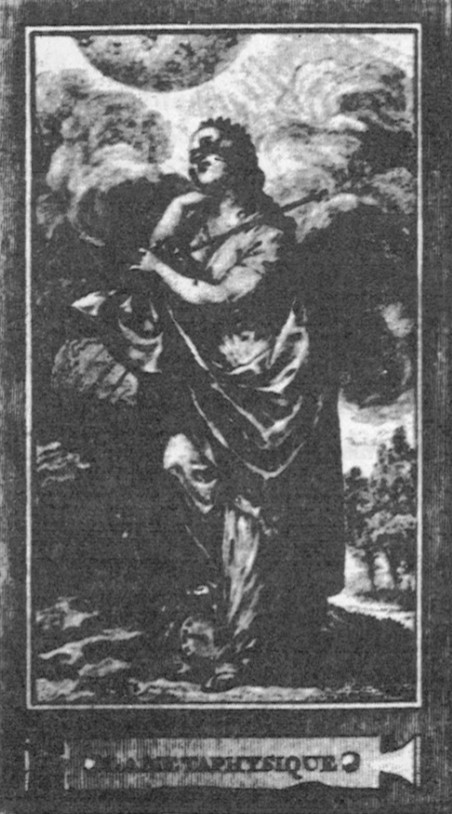
\includegraphics[scale=0.3]{./27_metaphysique/092}
\end{center}
\end{minipage}
\hfill
\begin{minipage}[c]{.45\linewidth}
\begin{center}
La métaphysique telle qu'on la représentait au
{\footnotesize XVIII}$^\text{e}$ siècle.
\end{center}
\vspace{0.31cm}

\hspace{0.91cm}{\it L'}Iconologie {\it de Cochin et Gravelot
(1796), d'où est extraite cette figure,
l'accompagne de ce curieux commentaire :
« Le bandeau placé au-dessous
de ses yeux, sans lui dérober la lumière d'en haut,
l'empêche seulement
de regarder vers le globe de la Terre ;
elle se couvre d'une partie de sa draperie
pour ne s'occuper que de la contemplation
des objets célestes. » On
remarquera aussi qu'elle foule aux
pieds une horloge, ce qui signifie sans
doute que son objet se situe en dehors
du temps.}
\end{minipage}

\section{Position actuelle du problème}% 331.
Bien qu'il ait été
ainsi posé en termes fort abstraits, le triple problème posé par Aristote
est loin d’être aujourd’hui périmé. — 1° D’abord, par delà les réalités
si variées dont la Science, à vrai dire, nous fait surtout connaître les
%581
modalités, il reste à la Métaphysique à s'interroger sur leurs essences
mêmes. Ainsi, savoir quelles sont les propriétés de tel ou tel corps
chimique, l’hydrogène ou le phosphore par exemple, est
un problème scientifique, et la Métaphysique n’a pas de
problème à se poser touchant ces corps en particulier. Mais
elle peut se poser un problème concernant l’essence de
la {\it Matière} en général. De même, il n’y a pas de problème
métaphysique qui se pose au sujet des fonctions
spéciales de la Vie comme la nutrition, la respiration,
le fonctionnement du système nerveux, etc. Mais il
y a un problème métaphysique concernant la nature,
l'essence même de {\it la Vie} en général. De même encore, la
Psychologie comme science étudiera chacune des fonctions
psychiques en particulier ; elle pourra même nous
donner une idée d’ensemble de la vie de l’esprit. Mais il
appartiendra à la Métaphysique de s'interroger sur la
nature intime de l'Esprit, sur ses rapports avec le
corps, etc. Ce sont précisément ces problèmes que nous
étudierons dans le chapitre suivant. — 2° Il en est de
même pour le problème des causes. Les causes que détermine
la Science (quand elle use de ce concept de {\it cause})
sont toujours des causes
{\it secondes}, c’est-à-dire qu’elles sont elles-mêmes les effets d’autres
%582
causes, et celles-ci à leur tour l’effet d’autres causes antérieures, et
ainsi de suite à l'infini. La Métaphysique est en droit de se demander
s’il est impossible de remonter jusqu’à une cause vraiment {\it première},
qui se suffise à elle-même et qui ne soit l’effet d'aucune autre cause.
3° Enfin il est un dernier problème qui semble appartenir à la Métaphysique
plus qu’à la Science : c’est celui de la {\it finalité}. On a vu
(\S 264, etc.) que, sauf peut-être dans certains cas spéciaux, comme
celui des Sciences biologiques (\S 276), la Science n’use guère de la
notion de {\it fin}. Elle est, en tous cas, incompétente pour résoudre le
problème des fins {\it dernières} de l’homme, c’est-à-dire de sa {\it destinée}
(tome II, chap. XXVI)

\section{Le fondement de la Connaissance}% 332.
Mais le problème
métaphysique peut aussi être posé sous une forme plus moderne, et,
cette fois encore, c’est la Science elle-même qui nous y conduit. La
Science, en effet, est {\it œuvre de l'esprit}. Mais l'esprit n’est pas ici un
simple « instrument ». Ce serait supposer que la Science a des fins
purement pratiques. Or on a vu qu’il n’en est rien : la Science est une
connaissance désintéressée (\S 238). Quelles que soient ses limites, que
nous venons de rappeler, elle a pour but de satisfaire un besoin proprement
intellectuel : le besoin de comprendre, et c’est en ce sens
qu’elle est une authentique « expérience spirituelle » (\S246). Les
Sciences physiques sont l’esprit s'imposant à la matière, au monde
extérieur, et les rendant compénétrables à l’intelligence humaine. Les
Sciences de l’homme sont la pensée ne se contentant plus de se « vivre »
elle-même, mais cherchant à se connaître vraiment, à se comprendre.
Or comment cela est-il possible? Comment l’esprit peut-il parvenir
à dominer la matière et à se comprendre lui-même? La pensée ne
semble-t-elle pas nous apparaître ainsi comme une {\it réalité première},
conformément au {\it Cogito}, au « Je pense, donc je suis » de Descartes qui,
après avoir révoqué en doute toutes les existences qu’il avait admises
jusque-là, s'aperçoit qu’il y a au moins une de ces existences qu’il ne
peut nier et qui est impliquée dans son doute même : l’existence de
sa propre pensée ? Le problème de l’Être nous apparaît ainsi comme
le fondement même du problème de la Connaissance. Pour que celle-ci
soit possible, pour que les choses soient compénétrables à la pensée,
ne faut-il pas que l'Être en son essence intime soit connaturel à la
pensée, qu’il soit de nature spirituelle ? — Ici encore, nous arrivons
à cette conclusion que la Science ne se suffit pas. Au delà de la Science,
nous apercevons l'{\it esprit} au-dessus de son ouvrage, l’esprit qui fait la
science elle-même. Nous nous plaçons donc dans une toute autre
%583
perspective, qui est celle de la Métaphysique, puisqu'il s’agit de la
nature même de l’Être en soi. Comme Hegel l’a dit de Descartes, en
posant la pensée comme réalité première, on « reprend tout par le
commencement » et la Science elle-même ne nous paraît désormais
définissable qu’en fonction de la pensée.

\section{Le fondement de l’Action}% 333.
Ce n’est pas seulement le
problème de la Connaissance qui nous conduit à la Métaphysique.
C’est aussi, on le verra au tome II, celui de l’Action. Certes, nous
disposons, pour diriger nos actes, de la connaissance morale qui, sous
sa forme spontanée, nous est fournie par la {\it conscience} (tome II,
chap. XIII). Celle-ci suffit le plus souvent à nous donner le sens des
{\it valeurs}, à nous permettre de discerner le bien du mal, à nous faire
connaître nos devoirs, etc. Elle peut d’ailleurs atteindre un niveau plus
élevé avec la {\it réflexion} morale et principalement la réflexion philosophique.
La Morale philosophique est précisément la théorie raisonnée
de ces {\it valeurs} qui nous sont d’abord données dans la conscience et
qui dirigent notre conduite.

Toutefois il faut, ici encore, se demander si le problème ne doit pas
être posé à un niveau supérieur. — {\it A.} Les valeurs, en effet, tout en
étant transcendantes à l’ordre des faits, de la réalité empirique, ne
sont pas gratuites : elles doivent avoir un {\it fondement}, et comment
pourraient-elles en avoir un si elles étaient sans point d’appui dans
l'ordre de l’Être ? C’est pourquoi la Morale, si elle peut et doit, en
première démarche, se constituer indépendamment de la Métaphysique,
requiert cependant, lorsqu'elle veut remonter jusqu’à ses principes
premiers, un fondement métaphysique (tome II, chap. XXV).
— {\it B.} Si d’autre part nous remarquons qu’il n’y a de valeurs que pour
une conscience et que, par suite, les valeurs sont essentiellement
{\it choses d’esprit} (\S 18, et t. II, chap. XIII), il nous apparaît que la notion
de la primauté de l’esprit s’impose ici comme à propos de la connaissance
pure et que la métaphysique qui convient ici, ne peut être
qu’une {\it philosophie de l'esprit}.

\section{Caractère de la connaissance métaphysique}% 334.
Ainsi définie, la connaissance métaphysique ne diffère pas seulement de la
connaissance scientifique (et aussi, on le verra au tome II, de la
réflexion morale) par sa {\it généralité} plus élevée, par l’{\it esprit de synthèse}
qu’elle requiert, plus impérieusement encore que celle-ci. Elle en
diffère aussi par le fait que, ainsi que l’ont fait observer plusieurs
philosophes contemporains, les problèmes métaphysiques sont ceux
%584
où « le questionneur comme tel est lui-même pris dans la question »
(Heidegger)
{\scriptsize (L'idée avait déjà été indiquée dès 1910 par Lawrence-Pearsall
Jacks dans {\it The Alchemy of Thought})}
ou encore, comme l'écrit Jean Wahl, où « le problème
empiète sur nous-mêmes », de telle sorte qu’ « en même temps que les
questions que le philosophe pose, portent sur un horizon très général,
il est pris lui-même dans cet horizon. »

Une telle connaissance ne saurait donc être le fruit d’une pure
construction conceptuelle, et l’on s’explique sans peine que, lorsqu'il
s’agit de tels problèmes, Bergson (\S 326) ait récusé l'intelligence
discursive et préconisé à sa place une {\it intuition} qui nous permettrait
de « coïncider avec » l'élan même de la vie et de saisir la spontanéité
créatrice immanente à l’être. Certains auteurs contemporains sont
d’ailleurs allés plus loin encore. Cette aptitude métaphysique qui est
refusée à l'intelligence, ils l’ont attribuée au sentiment : « Le sentiment,
écrit J. Wahl, n'est-il pas tendance vers ce qui le comble, vers l’autre
que lui ? Transcendance et sentiment sont unis par nature, bien plus
que transcendance et raison le furent jamais. » Et le même auteur soutient
que la Poésie s'apparente à la Métaphysique parce qu’elle aussi
nous fait saisir l’universel, quoique sous une forme subjective et non
conceptuelle.

De fait, on peut dire que, depuis toujours, la pensée humaine, au
lieu d'emprunter, pour atteindre l’absolu, les voies austères et parfois
décevantes de la connaissance intellectuelle qui laisse encore le {\it sujet}
connaissant en dehors de l’{\it objet} connu, a prétendu surmonter cette
dualité par la « possession intime et complète de l’objet ». Si l’on en
croit Lucien Lévy-Bruhl, c’est ce besoin d’une {\it communion} totale,
d’une {\it fusion} avec l’objet à connaître qui fait « le ressort principal des
doctrines dites anti-intellectualistes. Ces doctrines reparaissent périodiquement,
et à chaque réapparition elles retrouvent faveur. Car elles
promettent ce que ni la science positive pure ni les autres doctrines
philosophiques ne peuvent se flatter d’atteindre : le contact intime et
immédiat avec l'être, par l'intuition, par la compénétration, par la
communion réciproque du sujet et de l’objet, par la pleine participation,
en un mot, que Plotin a décrite sous le nom d’extase. » Besoin
qui, selon Lévy-Bruhl, demeure, chez l’homme, « plus impérieux et
plus intense que le besoin de se conformer aux exigences logiques »,
car « il est plus profond, il vient de plus loin », il vient des origines
mêmes de l’humanité.

%585
Mais nous avons vu ci-dessus (\S 326, fin) quelles difficultés soulève
la notion d’{\it intuition}, en tant que voie d'accès à la Métaphysique.
Quant au {\it sentiment}, ne faut-il pas dire plutôt, avec le psychologue
Henri Delacroix : « Le sentiment intercepte la réalité et se donne
l'apparence d’une réalité. Mais il n’est pas créateur, il n’est pas une
intelligence ou un équivalent de l’intelligence... Il n’y a rien dans le
cœur qui ne passe par l'esprit. » Peut-on d’ailleurs parler encore de
{\it connaissance} lorsque le sujet {\it s’absorbe} dans l’objet ?

En réalité, ce qu’exige, nous semble-t-il, la connaissance métaphysique,
c’est, au point de départ, un contact intime avec l'être, disons
mieux : une {\it participation} à l'être. C’est ce que nous fournit précisément
l'intuition du {\it cogito} : par cette intuition — intellectuelle en
même temps qu’existentielle — nous saisissons immédiatement notre
participation à la pensée, à la réalité spirituelle, laquelle d’ailleurs
(\S 358-359) est à la fois {\it être} et {\it valeur}. Mais, à partir de là, la Métaphysique,
désormais en prise sur l’être, peut s’édifier par une dialectique
qui ne sera plus pure construction de concepts, mais développement
de cette intuition fondamentale. « La Métaphysique, écrit Étienne
Gilson, est science à partir du point où, s’étant saisie du principe,
elle commence d’en déduire les conséquences ; mais le sort de la
doctrine se joue sur l’intellection du principe... L’aptitude du principe
à éclairer le réel sous tous ses aspects en confirmera sans doute la
vérité à mesure que se construira la doctrine ; mais c’est l’évidence
propre du principe, vu par l’entendement dans l’acte même de le
concevoir, qui en fait essentiellement la certitude. Quand on a saisi le
sens du principe, le déroulement de la doctrine se fait à sa lumière :
il n’en fait pas la vérité, il ne fait que la manifester. » — C’est ce
cheminement que nous essaierons de suivre dans les deux prochains
chapitres, spécialement dans le chapitre XXIX.

{\footnotesize 
\section{Sujets de travaux}% SUJETS DE TRAVAUX

{\bf Exercices.} — {\it Distinguer et classer les différents sens du mot métaphysique
et de ses dérivés dans les citations suivantes} : « On nomme métaphysique ce
qui surpasse la nature et qui est au-delà de la causalité et du langage »
(Erennios, néo-platonicien, IIIe siècle) ; « Elle est dicte métaphysique en
tant qu’elle considère {\it ens} l’être et les choses qui ensuivent à lui » (Christine
de Pisan) ; « Les choses métaphysiques, lesquelles ne dépendent point des
sens » (Descartes) ; « La façon dont il [Desargues] commence son raisonnement
en l’appliquant aux lignes droites et aux courbes est d'autant plus
belle qu’elle est plus générale et semble être prise de ce que j'ai coutume de
nommer la Métaphysique de la Géométrie » (Id.) ; « Il [Leibniz] saisissait
dans tout les principes les plus élevés et les plus généraux, ce qui est le
caractère de la métaphysique » (Fontenelle) ; « La métaphysique a cela de
%586
bon qu’elle ne demande pas des études préliminaires bien gênantes : c’est là
qu’on peut tout savoir sans avoir rien appris » (Voltaire) ; « Le vivant et
l’animé, au lieu d’être un degré métaphysique des êtres, est une propriété
physique de la matière » (Buffon) ; « Je veux mourir s’il y a dans toutes
ces têtes-là [celles des peintres] le premier mot de la métaphysique de leur
art » (Diderot) ; « On peut regarder la métaphysique comme un grand pays
dont une petite partie est riche et bien connue, mais confine de tous côtés
à de vastes déserts » (d'Alembert) ; « Je ne sais quelle métaphysique du
cœur s’est emparée de nos théâtres » (Id.) ; « Une connaissance métaphysique,
c’est-à-dire une connaissance qui dépasse l’expérience, ne doit contenir
que des jugements {\it a priori} » (Kant) ; « Comme la théologie, la métaphysique
tente d’expliquer la nature intime des êtres, l’origine et la destination de
toutes choses ; mais, au lieu d’y employer les agents surnaturels proprement
dits, elle les remplace par des {\it entités} ou abstractions personnifiées » (Comte) ;
« S'il existe un moyen de posséder une réalité absolument au lieu de la
connaître relativement, de se placer en elle au lieu d'adopter des points de
vue sur elle, la métaphysique est cela même. La métaphysique est la science
qui prétend se passer de symboles » (Bergson) ; « Un philosophe n’est pas
philosophe s’il n’est métaphysicien ; et c’est l’intuition de l'être qui fait le
métaphysicien » (Maritain) ; « Déraciner l'interprétation d’après laquelle
le besoin métaphysique serait comme une curiosité transcendante : c’est
plutôt un appétit, l'appétit de l’être. Il vise à la possession de l'être par la
pensée » (G. Marcel) ; « L'homme tel que la métaphysique nous le présente,
cest-à-dire comme un {\it étant}... » (Heidegger) ; « La métaphysique est liée
à l’être et au tout, mais non pas comme idées, bien plutôt à l'être et au tout
comme sentiments » (J. Wahl).

{\bf Exposés oraux.} — 1. La « philosophie première » d’après Aristote (voir
Ravaisson, {\it Essai sur la métaphysique d' Aristote} ; Cl. Piat, {\it Aristote}, liv. I,
chap. I). — 2. La métaphysique d’après Descartes (cf. préface des {\it Principes}
et {\it Méditations}). — 3. La conception existentielle de la métaphysique (voir
les textes de G. Marcel, Heidegger et J. Wahl).

{\bf Discussion.} — Le rôle du sentiment dans la connaissance métaphysique.

{\bf Lectures.} — {\it a.} L. Liard, {\it La Science positive et la Métaphysique}, 1879.
— {\it b.} A. Fouillée, {\it L'Avenir de la Métaphysique} fondée sur l'expérience,
1889. — {\it c.} H. Bergson, {\it Introduction à la Métaphysique}, dans la R. M. M.,
janv. 1903, p.1 (reproduit dans La Pensée et le Mouvant, p. 201). —
{\it d.} Ch. Dunan, {\it Légitimité de la Métaphysique}, ibid., sept. 1906, p. 651. —
{\it e.} H. de Keyserling, {\it La réalité métaphysique}, ibid., juill. 1911, p. 467. —
{\it f.} L. Lavelle, {\it La Présence totale}, Aubier, 1934. — {\it g.} G. Marcel, {\it Journal
métaphysique}, n.r.f., 1935 (spéc. p. 279-284) ; et {\it h. Le mystère de l'être}, Aubier,
2 vol., 1951. — {\it i.} M. Heidegger, {\it Qu'est-ce que la Métaphysique ?}, trad. fr.,
Gallimard, 1938 (texte difficile). — {\it j.} J. Wahl, {\it Existence humaine et
transcendance}, Baconnière, 1944 (notamment p. 78 : {\it Poésie et Métaphysique}) ;
{\it k. Note sur la Métaphysique}, dans la R. M. M., oct. 1947, p. 228 ; et {\it Traité
de Métaphysique}, 1957 ; {\it l.} G. Gusdorf, {\it Traité de Métaphysique}, A. Colin,
1956 ; {\it m.} Fr. D'Hautefeuille, {\it Les problèmes éternels de la Métaphysique},
La Colombe, 1961. — {\it n.} E. Gilson, {\it Introduction à la philosophie chrétienne},
Vrin, 14962. — {\it o.} G. Gusdorf, {\it Mythe et métaphysique}, Flammarion, 1963.
— {\it p.} J. Wahl, {\it L'expérience métaphysique}, Flammarion, 1965. — {\it q.}
L. Lavelle, {\it Science, esthétique, métaphysique}, A. Michel, 1967, 3e partie.
}

%
\chapter{La matière, la vie, l'esprit}

%chapitre XXVIII
%LA MATIÈRE, LA VIE, L'ESPRIT
%SOMMAIRE
%335. Matière, Vie, Esprit. — 336. Le Matérialisme. — 337. Le Matérialisme
%mécaniste. — 338. Le Matérialisme dialectique. — 339. Discussion du Matérialisme.
%— 340. Qu'est-ce que la Matière ? — 341. Le Vitalisme, — 342. Le
%Vitalisme antique. — 343. La médecine vitaliste. — 344. Le Vitalisme romantique.
%— 345. Le Vitalisme bergsonien. — 346. Le néo-vitalisme contemporain.
%— 347. Discussion du Vitalisme. — 348. Le Spiritualisme : de l’âme à
%l'esprit. — 349. Le Spiritualisme cartésien. — 350. Le Spiritualisme contemporain,
%— 351. Les rapports de l'esprit et du corps.

\section{Matière, Vie, Esprit}% 335. 
Le monde dans lequel nous
sommes plongés nous paraît se ramener à trois ordres de réalité que
nous désignons par les trois termes : matière, vie, esprit. L’Idéalisme,
interprété comme doctrine ontologique, prétendait ramener ces trois
réalités à une seule : la dernière. Mais cette réduction nous a paru
difficilement acceptable et ruineuse pour l’objectivité de la connaissance.
Comment dès lors définir ces trois ordres de réalité ? Comment
concevoir leurs rapports ? Une réduction en un autre sens serait-elle
possible? Enfin, si tout ne peut se réduire à l’esprit, ne faut-il pas
cependant affirmer l’irréductibilité et l'indépendance de l'esprit
lui-même ?

\section{Le Matérialisme}% 336.
Le Matérialisme est précisément la
doctrine qui prétend réduire tous les ordres de réalité à la matière.
Il ne doit pas être confondu avec le {\it Réalisme}. On a vu qu’il y a un
réalisme de l’intelligible : c’est le cas du réalisme platonicien et même,
en un sens (\S 111 B), du réalisme cartésien. Le Réalisme n'implique
d’ailleurs pas nécessairement la négation de la pensée comme fonction
propre et originale de l'esprit. Le {\it Matérialisme} est au contraire un
\textbf{\textit {monisme}} qui ne reconnaît qu’un seul ordre de réalités ou, comme on
dit de {\it substances} (voir \S 361), les substances matérielles. En ce sens,
il est l’antithèse exacte de l’{\it Idéalisme} qui est, lui aussi, {\it un monisme},
%588
puisqu'il ramène tout à l’existence unique de la pensée. Mais il
s'oppose aussi au {\it Spiritualisme} qui affirme l'indépendance de l'esprit.
— Le Matérialisme a pris plusieurs formes au cours de l’histoire. Il
peut reposer, notamment, sur une {\it non-distinction} du matériel et du
spirituel ou bien sur une réduction {\it consciente} de celui-ci à celui-là.
C'est ce dernier seul qui constitue le Matérialisme proprement dit
et qui répond à la définition d’Aug. Comte : « {\it Le Matérialisme est la
doctrine qui prétend expliquer le supérieur} [c’est-à-dire le plus
complexe] {\it par l’inférieur} [c’est-à-dire le plus simple]. » Le premier,
au contraire, où le spirituel n’est {\it pas encore distingué} du matériel est
l'{\it Hylozoïsme} des premiers philosophes grecs et des Stoïciens : nous en
traiterons à propos du Vitalisme (\S 342). Le Matérialisme proprement
dit peut prendre à son tour une forme {\it statique} : c’est le Matérialisme
mécaniste, ou une forme {\it dynamique} : c’est le Matérialisme dialectique
de la doctrine marxiste.

\section{Le Matérialisme mécaniste}% 337.
{\it A.} Dans l'antiquité, le
premier est représenté par les \textbf{\textit {Atomistes}} : Leucipe, Démocrite,
Épicure, qui réduisent tout ce qui existe aux {\it atomes}, conçus comme
de petites particules indivisibles, et à leurs mouvements dans le {\it vide}.
Selon Démocrite, l’âme se compose d’atomes, comme les corps;
mais, principe de vie et de mouvement, elle est faite d’atomes plus
légers et plus subtils. Plus tard, Épicure reprend cette doctrine,
avec des visées non plus scientifiques, mais morales ; et Lucrèce
la développe en latin dans son poème {\it De rerum natura}.

\vspace{0.24cm}
{\footnotesize Dans une lettre à un disciple, Épicure explique que l’âme est nécessairement
corporelle : car il n'y a d'incorporel que le vide ; or « le vide ne peut ni
agir ni pâtir » ; une âme incorporelle n'aurait donc ni activité ni sensations.
Elle est comparable à « un souffle mêlé d’une certaine quantité de chaleur
et répandu dans tout l'organisme ». La perception est produite par des
« simulacres », images extrêmement petites « détachées des objets et reproduisant
leurs formes et leurs couleurs » et qui, entrant « dans nos yeux et
notre pensée » avec un mouvement très rapide, « produisent par leur accumulation
l'apparence d’un objet unique et permanent ». — En reprenant ces
théories, Lucrèce distingue cependant entre l'âme ({\it anima}) et l'esprit
({\it animus}). La première, étant, comme l'avait dit Épicure, répandue dans
tout le corps, ne peut être le siège des pensées et des sentiments, indépendants
du corps. Ceux-ci doivent donc être rapportés à un esprit localisé dans le
cœur, où nous les sentons.}
\vspace{0.31cm}


Dans l'intention d’Épicure et surtout de Lucrèce, ces théories ont
pour but d’apaiser l'angoisse humaine et la crainte de la mort, provoquées
par les croyances populaires à l’au-delà. C’est en effet une
caractéristique du Matérialisme proprement dit de s'opposer, le plus
%589
souvent, aux croyances religieuses. Au {\footnotesize XVII}$^\text{e}$ siècle cependant,
Gassendi (1592-1655) reprendra à son compte l’atomisme d’Épicure
et sa théorie matérialiste de l’âme, mais en y superposant la notion
d’une âme spirituelle, capable de raison et de volonté libre, et celle
d’un Dieu créateur. 

{\it B.} Le \textbf{\textit {Mécanisme cartésien}} devait, au {\footnotesize XVIII}$^\text{e}$ siècle surtout,
conduire certains philosophes jusqu’au Matérialisme. Définissant la
matière par l'étendue (\S 111 B), Descartes avait expliqué par « la
figure et le mouvement » toutes les propriétés physiques des corps
et il n’avait pas craint d’étendre cette interprétation {\it mécaniste} aux
organismes vivants : notre corps est une {\it machine} gouvernée par une
âme ; mais les animaux, qui n’ont pas d’âme, sont de pures machines.
Certes, Descartes, spiritualiste, avait réservé les droits de l’âme
humaine. Mais, au {\footnotesize XVIII}$^\text{e}$ siècle, certains auteurs s’autoriseront de
sa doctrine mécaniste pour la généraliser à tout l’être de l’homme.

\vspace{0.24cm}
{\footnotesize C'est ainsi que le médecin La Mettrie, dans son {\it Homme-machine} (1748),
ne reproche à Descartes que d’avoir, dans sa théorie des animaux-machines,
refusé la sensibilité aux bêtes et d’avoir admis chez l'homme deux substances
là où une seule suffisait. D'Holbach écrit de même dans son {\it Système
de la nature} (1770) : « Descartes est le premier qui ait établi que ce qui
pense doit être distingué de la matière. D'où il conclut que notre âme ou
ce qui pense en nous est un esprit. N’eût-il pas été plus naturel de conclure
que, puisque l’homme qui est matière et qui n’a d’idées que de la matière,
jouit de la faculté de penser, {\it la matière peut penser ?} » L'homme, en effet,
est « un être purement physique » et tout, en lui, provient de sa sensibilité
physique. C'était aussi le principe du livre d'Helvétius, {\it De l'esprit} (1758).
Les mêmes thèmes se retrouvent également chez Diderot.}
\vspace{0.31cm}


{\it C.} Au {\footnotesize XIX}$^\text{e}$ siècle, le Matérialisme va prendre une allure un peu
différente du fait de sa liaison avec la \textbf{\textit {Physiologie.}} Mais, celle-ci en
étant encore, au début du siècle, à ses premiers pas, cette influence
ne le modifiera pas profondément. Dès 1796, c’est Cabanis qui, dans
son {\it Histoire physiologique des sensations}, lance la formule fameuse :

\vspace{0.24cm}
{\footnotesize « Pour se faire une idée juste des opérations de la pensée, il faut considérer
le cerveau comme un organe particulier destiné à la produire, de
même que l’estomac et les intestins à faire la digestion, le foie à filtrer la
bile... Le cerveau digère en quelque sorte les impressions ; il fait organiquement
la sécrétion de la pensée. »}
\vspace{0.31cm}


En Allemagne, à partir de 1850, toute une école de médecins et
de naturalistes prétend, en présentant la pensée comme une {\it fonction
du cerveau}, parler au nom de la science. Les théories de l’évolution,
interprétées dans le sens d’une évolution linéaire à partir d’une hypothétique
« monère » primitive, viennent ici appuyer le matérialisme.

%590
\vspace{0.24cm}
{\footnotesize Karl Vogt (1817-1895) utilise le darwinisme ; il aggrave la formule de
Cabanis en disant : « Le cerveau sécrète la pensée comme le foie sécrète la
bile et les reins l'urine. » Louis Büchner, dans son ouvrage {\it Force et Matière}
(1855) qui eut alors un énorme retentissement, soutient un matérialisme
mitigé qui présente la pensée comme un produit de la matière sans qu'elle
soit elle-même matière ; il distingue en effet, de façon assez obscure, la
{\it matière} de la {\it force}. Le hollandais Moleschott (1822-1893), Henri Czolbe
(1819-1873), Du Bois-Reymond, célèbre par son {\it ignorabimus} (nous ignorerons
toujours ce que c’est que la force, ce que c'est que la matière, et
comment elles peuvent penser : 1872), défendent des thèses analogues.
Ernest HæckeL ({\it Les Énigmes de l'univers}, 1899) soutient un « monisme »
inspiré du darwinisme au sens le plus dogmatique.}
\vspace{0.31cm}


On peut enfin rattacher au Matérialisme la théorie \textbf{\textit {épiphénoméniste}}
de la conscience, qui fait de celle-ci un simple « reflet » de l’activité
cérébrale sans action sur notre comportement (voir \S 31 B). Elle a été
surtout soutenue, elle aussi, par des physiologistes ou des médecins.
{\scriptsize (On peut considérer la {\it Cybernétique} comme une forme nouvelle de
l'épiphénoménisme : nous en avons dit quelques mots ci-dessus \S 31 B.)}

\vspace{0.24cm}
{\footnotesize Ce fut le point de vue des Anglais Thomas Huxcey (1825-1895) et Henry
Maudsley (1835-1918) et, en France, de Félix Le Dantec (1869-1917)
qui l’a présenté sous sa forme la plus absolue, tout en admettant que « les
éléments des substances brutes ont leur conscience élémentaire ». Ce fut
également, en Amérique, celui du naturaliste Jacques LœB (1859-1924) et
des psychologues {\it behavioristes} (J.-B. Watson, A.-P. Weiss, R.-B. Perry)
qui définissaient l'esprit « l’ensemble des réactions de l'organisme sur son
milieu » et proclamaient la « stérilité » de la conscience.}
\vspace{0.31cm}


\section{Le Matérialisme dialectique}% 338.
Il ne faut pas confondre
le {\it Matérialisme dialectique} avec le Matérialisme mécaniste. On a vu
au \S 299 B que K. Marx a été amené à concevoir sa doctrine par
réaction contre celle de Hegel. Chez Hegel, écrira-t-il plus tard,
« la dialectique marche sur la tête : il suffit de la remettre sur ses
pieds pour lui donner une physionomie raisonnable », En effet, « pour
Hegel, le mouvement de la pensée qu’il personnifie sous le nom de
l’Idée, est le démiurge de la réalité, laquelle n’est que la forme phénoménale
de l’Idée. Pour moi, au contraire, dit Marx, le mouvement
de la pensée n’est que la réflexion du mouvement réel, transporté et
transposé dans le cerveau de l’homme ». A son origine, le Matérialisme
dialectique est donc surtout un {\it Réalisme} qui s’oppose à l’Idéalisme
hégélien. Mais il est aussi un {\it humanisme} anti-religieux qui s'inspire
de celui du néo-hégélien Feuerbach (1804-1872).

\vspace{0.24cm}
{\footnotesize Comme celui-ci, Marx fait grief à la religion d’« aliéner» l'homme, c’est-à-dire
d’être une idéologie illusoire qui situe l’homme en dehors de lui-même
et le détourne de ses activités réelles. Mais, au matérialisme de Feuerbach
%591
comme à celui du {\footnotesize XVIII}$^\text{e}$ siècle, Marx reproche : 1° d’être purement {\it statique} :
l’objet, le réel y est posé comme un donné, et non comme la base d’une
activité de l’homme, d’une « praxis » ; or, dit Marx, « les philosophes n'ont
fait qu'interpréter le monde ; il s’agit maintenant de le changer » ; 2° de
{\it méconnaître l'histoire} : il n’y a pas d’essence absolue de l’homme ; « l’histoire
tout entière n’est qu’une transformation continue de la nature humaine » ;
3° d'admettre un {\it déterminisme mécanique} qui fait de la pensée une simple
fonction du cerveau et de l’homme un produit des circonstances, notamment
de l’éducation : il oublie ainsi 4 que les circonstances sont transformées
par l’homme et que l’éducateur lui-même doit être éduqué» ; en outre, les
conditions sociales de la pensée ne sont pas moins importantes que les
conditions physiologiques.}
\vspace{0.31cm}

A cette époque (1844-45), Marx écrit que, « dans l’état de société,
le subjectivisme et l’objectivisme, le spiritualisme et le matérialisme
perdent leur opposition et, par suite, leur existence » et que « la vieille
opposition du spiritualisme et du matérialisme a été partout mise
de côté » par Feuerbach. Par la suite, à la fois sous l'influence des
nécessités polémiques, comme l’a dit Fr. Engels, et des théories
darwiniennes où Marx crut trouver une confirmation de ses idées, la
doctrine marxiste s’étrécit en un Matérialisme strict où toute la vie
spirituelle de l’homme, discréditée sous le nom d’{\it idéologie}, apparaît
trop souvent comme un simple « reflet », plus ou moins illusoire, des
conditions économiques, spécialement de l’état des {\it forces productives
matérielles} à un moment donné de l’histoire. Toutefois, ainsi qu’il a
déjà été remarqué à propos du Matérialisme historique (\S 299) qui
n’est que l’application au devenir humain du Matérialisme dialectique,
ce dernier n’est pas, comme on le dit parfois, un {\it économisme} exclusif :
il fait place aux autres facteurs du développement humain, même
aux facteurs {\it idéologiques} auxquels il attribue une {\it action en retour}
sur la base économique. En outre, la pensée profonde de Marx semble
bien avoir été que l’activité économique elle-même n’est pas d’ordre
purement matériel, puisque le travail, par exemple, implique une
représentation {\it idéale} du résultat à obtenir.

\section{Discussion du Matérialisme}% 339.
Deux critiques fondamentales
peuvent être adressées au Matérialisme.

{\it A.} La première
est que la réduction qu’il prétend opérer de la vie spirituelle à ses
conditions matérielles cst inintelligible.

\vspace{0.24cm}
{\footnotesize N'insistons pas sur la forme que Cabanis, K. Vogt, etc., lui ont donnée
en affirmant que la pensée n’est qu’une {\textit{\textsf{sécrétion}}} du cerveau. Büchner
lui-même critique cette formule ; et, de fait, comment comparer avec une
sécrétion, qui est quelque chose de sensible, de pondérable, de localisable
dans l’espace, la pensée, qui ne tombe pas sous les sens, qui n’est ni pondérable
%592
ni localisable ? Au reste, le cerveau n’est pas une glande, et c’est un
non-sens physiologique de lui attribuer une « sécrétion ». Il ne vaut guère
mieux de dire, avec les {\it épiphénoménistes}, que la pensée est un {\textit{\textsf{reflet}}} de ce
qui se passe dans le cerveau. Le terme de « reflet » n’est qu’une métaphore
qui n’a aucun sens précis et qui n’est pas plus heureuse que les termes de
{\it lueur}, de {\it phosphorescence}, etc., qu'ont employés parfois les mêmes auteurs
pour désigner la pensée. — A peine serait-il moins impropre de parler de
la pensée comme d’une \textsf{\textit {fonction}} du cerveau. D'abord, on a vu (cf. \S 28-30) que
ni les physiologistes ni les psychologues ne conçoivent plus ainsi le rôle du
cerveau. La pensée est liée à l’ensemble de notre {\it action}, de nos {\it comportements},
et le cerveau a pour fonction d’être l'organe {\it régulateur} de ces comportements,
non pas du tout de fabriquer, en quelque sorte, de la pensée : « Un
cerveau séparé de l’être vivant est incapable de pensée et d'action. Le cerveau
est un des éléments d’un circuit extrêmement complexe que nous appelons
{\it l’action}. En réalité, l'homme pense avec tout son corps : il pense avec ses
mains, ses pieds, ses oreilles, aussi bien qu’avec son cerveau. Il est absolument
ridicule de dire que sa pensée dépend d’une partie de lui-même : c'est
comme si on disait que notre habileté manuelle dépend de nos ongles.
L'activité psychologique est une activité d'ensemble, et non pas une
activité locale. {\it Le cerveau est tout simplement un ensemble de commutateurs} »
(Pierre Janet). — D'autre part, une {\it fonction} est une \textsf{\textit {abstraction}}, qui désigne
simplement un ensemble d'opérations des organes. La pensée est une
{\it réalité concrète} et, qui plus est, c’est une réalité {\it qui se connaît elle-même},
c’est une réalité {\it pour-soi}. Là est la difficulté majeure à laquelle se heurtera
toujours, semble-t-il, le Matérialisme. On aura beau insister sur les {\it conditions}
physiologiques de la pensée, et notamment de la pensée consciente,
qu’il n’est d’ailleurs pas question de nier (voir \S 26-31) : on ne nous fera
jamais comprendre comment un phénomène matériel, quel qu'il soit,
pourrait engendrer ce quelque chose d’essentiellement nouveau qu'est la
{\it prise de conscience} par soi-même de l'être pensant et même la {\it conscience}
simple. « La matière de demain, pas plus que celle d’aujourd’hui, écrivait
le psychologue A. Binet, ne peut engendrer que des effets matériels. » Et,
faisant allusion aux recherches d’un histologiste qui avait longuement étudié
les tissus cérébraux, Binet ajoutait : « C’est que l'étude, si patiente, si
minutieuse qu'on la suppose, de cet écheveau nerveux, ne pourrait jamais
nous faire connaître ce que c’est qu’un état de conscience, si nous ne le
savions déjà par ailleurs ; car ce n’est jamais dans le champ du microscope
qu’on voit passer un souvenir, une émotion ou un acte de volonté. »}
\vspace{0.31cm}

On peut même dire qu’il y a dans le Matérialisme une sorte de
\textbf{\textit {contradiction}} interne. Toute affirmation d’une réalité étrangère à
l'esprit implique déjà la pensée (c’est, on l’a vu, ce qu’il y a d’irréfutable
dans l’Idéalisme) ; et, s’il prenait fantaisie à la pensée de se nier elle-même,
ainsi qu’il arrive précisément, en un sens, dans le Matérialisme,
elle {\it s’affirmerait encore dans sa négation même} : car tout jugement
est œuvre de l’esprit.

\vspace{0.24cm}
{\footnotesize Ces objections valent contre le Matérialisme dialectique aussi bien que
contre le Matérialisme mécaniste. La théorie marxiste n'apporte en effet
ici rien d’essentiellement nouveau. Lorsqu'un Engels affirme : « Notre
conscience et notre pensée... ne sont que les produits d’un organe matériel,
%593
corporel, le cerveau. La matière n'est pas un produit de l'esprit : c'est
l'esprit qui est le produit supérieur de la matière », il ne fait que répéter
une formule un peu simple héritée du scientisme physiologique du début du
{\footnotesize XIX}$^\text{e}$ siècle. Lorsqu'un Lénine affirme : « L'univers n’est que matière
en mouvements, il en revient au Matérialisme mécaniste. Lorsque certains
théoriciens marxistes déclarent que la superstructure idéologique est « le
reflet » de la base matérielle, ils empruntent une métaphore bien creuse
à l'épiphénoménisme, que cependant ils repoussent.}
\vspace{0.31cm}

{\it B.} La seconde difficulté concerne la notion de \textbf{\textit {matière}} elle-même.
Cette notion est loin d’être aussi claire que certains matérialistes
semblent le supposer. Qu’on se rappelle toutes les difficultés
auxquelles s’est heurté le Réalisme vulgaire, celui précisément qui
identifie « le réel » avec la réalité sensible (\S110). Bien des matérialistes,
comme Du Bois-Reymond (1818-1896), ont avoué leur ignorance touchant
l’élément ultime de cette réalité. Beaucoup aussi, afin de pouvoir
expliquer, comme disait Comte, le supérieur par l’inférieur,
{\it mettent déjà dans celui-ci les propriétés de celui-là} : c’est ainsi que
D’Holbach, Diderot, etc., affirment que « la matière peut penser »
et que Le Dantec admet jusque dans les éléments chimiques une
conscience élémentaire, que Büchner déclare la {\it force} irréductible à la
matière, etc. Mais qu’est-ce que la « force » ? comment la matière peut-elle
penser ? que peut bien être la conscience d’une cellule, d’un atome,
d’un électron ? Avouons-le : ces formules sont aussi {\it dénuées de sens} que
celle des Atomistes de l’antiquité quand ils affirmaient que la pensée
est faite d’atomes subtils ! On glisse ici dans un véritable roman de
la matière, et l’on se paye de mots.

\vspace{0.24cm}
{\footnotesize Sans tomber dans un aussi grossier verbalisme, le Matérialisme dialectique,
ici encore, prête le flanc à une objection analogue. Tout, dans la vie
sociale, nous dit-on, se ramène, en dernière analyse, à l’action des « forces
productives ». Mais on a pu montrer récemment que, dans ses premiers
écrits, Karl Marx entend par là à peu près toutes les activités de l’homme,
y comprises même les « forces spirituelles », et plus tard, il continuera à
affirmer que l'acte producteur par excellence, le {\it travail}, contient un élément
idéal (\S 299 B 3°). Comment donc peut-on affirmer que la « base » est uniquement
matérielle ?}
\vspace{0.31cm}

\section{Qu'est-ce que la Matière ?}% 340.
Essayons donc de préciser la
notion de {\it matière}, et pour cela examinons rapidement son évolution
chez les philosophes et les savants.

{\it A. Dans l'antiquité}, la matière fut d’abord conçue comme animée :
c’est l’{\it Hylozoïsme} auquel nous avons déjà fait allusion et sur lequel
nous reviendrons (\S 342).

Les Atomistes sont peut-être les seuls qui aient eu, dans l’antiquité,
%594
une conception claire de la matière. C’est déjà une conception \textbf{\textit {géométrique}}
où seules les qualités primaires (\S 114) : l’étendue, la
pesanteur, la distribution dans l’espace, le mouvement, sont reconnues
réelles ; Démocrite précise que la cause du mouvement ne
réside pas dans une {\it force} extérieure aux atomes. Mais c’est aussi une
conception \textbf{\textit {discontinuiste}} puisque la matière se résout en particules
indivisibles.

\vspace{0.24cm}
{\footnotesize Platon ne nomme même pas la matière : « espèce obscure et difficile
à concevoir », dit-il lui-même de ce qu’il nomme « le réceptacle de tout
devenir ». — Cette conception se précise chez Aristote : il y a bien une
matière ({\it hylè}) dans les corps ; mais, pure « puissance », virtualité indéterminée,
{\it elle n'existe pas sans la forme}, sans la détermination des qualités
telles que le chaud, le froid, le lourd, le léger, etc. Elle est indestructible ;
car tout ce qui périt, se résout en elle.}
\vspace{0.31cm}

{\it B. Le Mécanisme cartésien}. Il faut arriver à Descartes pour
retrouver une conception claire de la matière, celle qui a déjà été
indiquée au \S 111 B : la matière est la {\it res extensa}, la « chose étendue » ;
toutes ses propriétés se ramènent à la
\textbf{\textit {figure}} et au \textbf{\textit {mouvement.}} Mais,
comme l’étendue est divisible à l'infini, il n’y a ni atomes ni vide :
cette conception \textbf{\textit {géométrique}} de la matière est en même temps une
conception \textbf{\textit {continuiste.}} Scientifiquement, elle se traduit par le principe
de la {\it constance de la quantité de mouvement} (produit m.{\bf v} de
la masse par la vitesse), base de toute la Physique cartésienne.

{\it C. Le Dynamisme leibnizien}. On a vu au \S 113 comment Leïbniz
a critiqué la conception cartésienne et comment il s’est efforcé de
réserver, dans sa doctrine idéaliste, une certaine place à la matière,
du moins comme principe de résistance ou de limitation de la perception
des monades. D’autre part, il avait découvert que ce n’est pas,
comme l’avait cru Descartes, la « quantité de mouvement », mais la
« quantité des forces vives » (définie par le produit $m.v^2$) qui demeure
constante : par là, Leibniz se trouvait beaucoup plus près du principe
moderne de la conservation de l’\textbf{\textit {énergie.}} Aussi se fait-il une conception
{\it dynamiste} de la matière elle-même. Celle-ci ne peut s’expliquer uniquement,
selon lui, par des propriétés mécaniques : comme toute
substance, elle est « force active », elle possède une « propriété agissante »,
et, « non plus que la substance spirituelle, ne cesse jamais d’agir ». Dès
1671, Leibniz réduisait l’opposition de l'esprit et de la matière en
disant que tout corps est une {\it mens momentanea}, une âme qui vit dans
l'instant, qui ne sait pas se souvenir, tandis que, dans l'esprit, l’effort
interne et l’action extérieure se conservent. Dans la {\it Monadologie},
il affirmera « qu’il y a un monde de créatures, de vivants, d’animaux,
%595
d’entéléchies
{\scriptsize ({\it Entéléchie}, du grec entélôs, parfaitement,
et {\it echein}, se trouver. Aristote avait
désigné par ce mot la pleine réalisation des virtualités d’un être. Leibniz l’applique aux
monades comme se suffisant à elles-mêmes en tant que sources de leurs états internes
(\S 113))},
d’âmes dans la moindre partie de la matière », à tel
point que celle-ci « peut être conçue comme un jardin plein de
plantes ct comme un étang plein de poissons ».

{\it D. La matière dans la science moderne}. Ces deux conceptions, cartésienne
et leibnizienne, ont trouvé un écho dans la science.

\vspace{0.24cm}
{\footnotesize Le mécanisme cartésien a inspiré toutes les théories dites \textsf{\textit {cinétiques}} qui
ont eu cours jusqu’au début du {\footnotesize XX}$^\text{e}$ siècle.
Dès 1690, Chr. Huyghens, en
posait le principe, en harmonie avec la Physique cartésienne, en disant que
les propriétés de la lumière ne peuvent s'expliquer que par « le mouvement
de quelque matière, au moins, ajoutait-il, dans la vraie philosophie, dans
laquelle on conçoit la cause de tous les effets naturels par des raisons de
mécanique ». Les théories {\it ondulatoires} ou {\it vibratoires} (\S 74) étaient toutes
des applications de ce principe. En 1900, au Congrès international de
Physique, un savant proclamait : « L'esprit de Descartes plane sur la
Physique moderne. Plus nous pénétrons dans la connaissance des phénomènes
naturels, plus se développe et se précise l’audacieuse conception
cartésienne : il n’y a dans le monde physique que de la matière et du mouvement. »
Un grand physicien anglais, lord Kelvin, déclarait que, pour lui,
comprendre un phénomène physique, c'est « pouvoir en faire un modèle
mécanique correspondant ».

La conception dynamiste de Leibniz est passée, elle aussi, dans le domaine
scientifique. Dès 1759, le P. Boscovich interprétait la notion de l'atome
comme celle d’un pur centre de forces. Mais ce furent surtout les découvertes
de l'{\it équivalent mécanique de la chaleur} (Mayer et Joule) et de la {\it dégradation}
de l'énergie (S. Carnot ct Clausius) qui permirent à Helmoltz (1847) de
dégager cette notion d'{\it énergie} et de créer l'\textsf{\textit {énergétique}}. La distinction de
l'{\it énergie cinétique} (correspondant à la notion leibnizienne de la « force vive »)
et de l'{\it énergie potentielle} permit de préciser la doctrine, bientôt exploitée
sur le terrain philosophique par le chimiste allemand Ostwald et le physicien
français Duhem. Selon Ostwald (1853-1932), toutes les qualités de la
matière se ramènent à {\it l'énergie} : le poids est une sorte d'énergie de position,
et la conscience elle-même est de nature énergétique : « l'énergie » apparaissait
ainsi comme la substance même du monde, comme une véritable
« chose en soi ». Ostwald s’imaginait avoir ruiné ainsi le Matérialisme dont,
en 1895, il proclamait la faillite définitive, sans s’apercevoir qu'il prêchait
lui-même une sorte de « Matérialisme métamorphosé » (H. Driesch). Pierre
Duhem (1861-1916) alla presque aussi loin en soutenant que c'est l'abaissement
de {\it tension} de l'énergie et sa dispersion, mesurés par le principe de
Carnot (entropie), qui caractérisent l’action matérielle.

Mais, vers la fin du {\footnotesize XIX}$^\text{e}$ siècle, on assistait déjà à un {\it recul de l'énergétisme}.
Dès 1912, Poincaré déclarait que « les anciennes hypothèses mécanistes
et atomistes [avaient] pris assez de consistance pour cesser de nous
apparaître comme des hypothèses ». Certes, l'{\it atome} des chimistes modernes
est bien différent de l'{\it atome} des anciens
{\scriptsize (Pour les anciens (Démocrite, Épicure), l'atome était l'élément dernier et indivisible
de la matière. Pour les savants modernes, l'atome est tout un monde qu'on a souvent
comparé à un {\it système solaire en miniature}, le noyau atomique formant le gentre de ce
système. « Chaque progrès de la physique, écrivait Poincaré, nous révèle une nouvelle
complication de l’atome » : c’est de plus en plus vrai aujourd’hui !)}
; mais, dès alors, il avait cessé d’être
%596
« une fiction commode » pour devenir « une réalité ». La théorie cinétique
ds gaz, appuyée de nombreuses théories analogues (théorie des solutions, etc.),
venait étayer la conception {\it discontinuiste} et {\it mécaniste} de la matière. Certes,
par la suite, les nouvelles théories physiques, spécialement celle de la Relativité
(\S 269), ont bouleversé bien des points de vue classiques. Mais, comme
l’observe P. Mouy, « s’il est vrai que la physique de notre temps a remplacé
la théorie de l’éther par celle de \textsf{\textit {champs}}
{\scriptsize (A la notion classique de l’espace neutre et infini, la théorie de la Relativité substitue
celle d'un {\it champ} doué de propriétés déterminées et fini, quoique illimité, l'espace
de Riemann (cf. ci-dessus \S 98 B et 269))}
abstraits, elle est au fond, et peut-être
sans le soupçonner, cartésienne », cartésienne à la façon de Malebranche
dont « l'étendue intelligible » (\S 111) était précisément un système de rapports
abstraits. — D'autre part, il apparaissait de plus en plus qu'il n'y
avait pas lieu d’{\it opposer} l'énergie à la matière pondérable. Celle-ci semblait
caractérisée autrefois par la notion de {\it masse}. Or « la nouvelle mécanique
affirme l’inertie de l'énergie, c'est-à-dire la variation de la masse d’un corps
proportionnellement à l’énergie interne de celui-ci, unissant en une seule les
deux notions de masse et d'énergie » (Langevin). — Enfin il se révélait que
matière et énergie sont de {\it structure} identique. On a vu (\S 268) que, lorsqu'il
s’est agi d'expliquer la structure du rayonnement lumineux, les théories
scientifiques, parties de la notion {\it discontinuiste} d’une {\it émission} corpusculaire,
durent en venir à une conception {\it continuiste}, celle des théories {\it ondulaloires},
mais que, depuis 1900, avec la physique {\it quantique}, s'est imposé un
retour partiel à la notion d'une structure « granulaire » de l'énergie lumineuse.
C’est de cette conception granulaire qu'étaient partis, à propos de
la matière, les Atomistes de l'antiquité, et l'on vient de voir que cette
conception s'était de plus en plus imposée, de nos jours, aux Sciences
physiques. Mais la Mécanique ondulatoire (\S 268 E) introduit au sein même
de l’atome des {\it ondes} associées aux corpuscules de matière (par exemple, aux
électrons). Ainsi, « pour la matière comme pour la lumière, l’aspect atomique
et discontinu des entités élémentaires se double d’un aspect continu
et ondulatoire » et, par suite, « matière et lumière apparaissent comme
beaucoup plus semblables dans leur structure qu'on ne le pensait autrefois » (L. De Broglie).}
\vspace{0.31cm}

Il résulte de tout cela que les Physiciens d’aujourd’hui se trouvent
assez embarrassés quand il s’agit de définir la matière. La chose
d’ailleurs n’est pas nouvelle. Déjà, dans le Discours préliminaire de
l'{\it Encyclopédie}, D'Alembert remarquait que plus les savants « approfondissent
l’idée qu’ils se forment de la matière et des propriétés qui
la représentent, plus cette idée s’obscurcit et paraît vouloir leur
échapper ». En 1909, H. Poincaré déclarait : « L’une des découvertes
les plus étonnantes que les physiciens aient annoncées dans ces
dernières années, c’est que la matière n’existe pas », et il se demandait
si, la matière se définissant par la {\it masse} et cette dernière notion se
trouvant compromise, il ne fallait pas conclure à {\it la fin de la matière}.

%597
Depuis lors, le problème n’a fait que se compliquer. L. de Broglie
écrivait en 1946 : « Si j'étais un humoriste, je dirais qu'ayant passé
notre vie à étudier les atomes, nous ne savons plus du tout ce que
c'est. »

{\it E. Conclusion}. On voit donc que la notion même de {\it matière} est
sujette à discussion. La matière, a-t-on dit (M. Lodetti), n’est pas
une substance, mais « une relation aux œuvres humaines : il n’y a
de matière que pour le travail. » Elle n’est même pas, comme l’a
voulu Bergson (cf. \S 345), une sorte de dégradation de l’être : « La
matière ne provient pas d’un esprit ou d’un être originel qui tombe de
lui-même et se dégrade, elle est {\it une image} issue de la conduite des
hommes qui, considérant l’être par rapport à des projets, l’utilisent
en vue de leurs réalisations » (Id.). En ce sens, on peut dire que la
matière est « imaginaire ».

\section{Le Vitalisme}% 341.
Le Vitalisme, au sens philosophique du
terme, peut être considéré comme une doctrine {\it intermédiaire} entre
le Matérialisme et le Spiritualisme et qui s'apparente parfois de
façon assez étrange à l’un et à l’autre. Il consiste à faire de \textbf{\textit {la Vie}}
une entité qui forme une {\it totalité} indivisible et qui se montre rebelle
aux analyses de l'intelligence. Tantôt cette réalité se confond avec
la pensée, tantôt elle s’en distingue. Mais, même en ce dernier cas,
il y a \textbf{\textit {continuité}} entre la vie et la pensée.

\section{Le Vitalisme antique}% 342.
Dans l'Antiquité, le Vitalisme
va parfois jusqu’à l’\textbf{\textit {hylozoïsme}} (grec : {\it hylè}, matière; {\it zôon}, être
vivant), c’est-à-dire jusqu’à une conception de l’univers qui en fait
un organisme, un être vivant.

\vspace{0.24cm}
{\footnotesize {\it A.} C'est ainsi que les premiers philosophes grecs distinguent encore
fort mal le {\it matériel}, le {\it vital} et le {\it spirituel}. Thalès qui considère l’eau,
l'élément marin, comme l’élément primordial et la substance même du
monde, lui attribue une âme, c’est-à-dire un principe de mouvement et,
sans doute, de vie : « Toutes les choses, dit-il, sont pleines de dieux. » Pour
Héraclite, c'est le feu qui est le principe premier, mais c’est un feu
« éternellement vivant », d'où naissent les âmes. Ames et corps représentent
divers degrés de tension, comme les cordes d’une lyre. Déjà Héraclite dépeint
l’univers comme quelque chose d’essentiellement {\it mouvant} et il s'oppose
à la conception des Pythagoriciens « d’après laquelle on pourrait expliquer
l’univers au moyen d'unités mathématiques indivisibles et fixes que
l'on combinerait ensemble » (R. Berthelot). Beaucoup de ces traits se
retrouveront jusque dans les doctrines modernes.}
\vspace{0.31cm}

{\it B.} Platon considère l’âme comme un \textbf{\textit {principe de mouvement}} :
elle est « ce qui se meut soi-même ». Mais elle est, en même temps,
parente des Idées et l’on verra (\S 348) que par là Platon annonce le
%598
spiritualisme proprement dit. — Aristote professe un \textbf{\textit {finalisme,}}
beaucoup plus proche du vitalisme. La « nature » ({\it physis}) est pour lui
ce qui a son principe moteur en soi-même, alors que les produits de
l'art ({\it technè}) viennent d’un principe extérieur. La nature est donc
\textbf{\textit {forme}} et, en un sens, \textbf{\textit {âme}} :
on a vu en effet (\S 340 A) que la matière,
selon Aristote, ne serait rien sans la forme ; et, d’autre part, c’est
l’âme qui est {\it la forme du corps}. Il y a trois espèces d’âmes, correspondant
aux trois formes de la vie dans l’univers : l’âme {\it végétative} ou
{\it nutritive}, la seule que possèdent les plantes ; l'âme {\it sensitive}, qui est aussi
{\it motrice}, privilège des animaux ; et enfin l’âme {\it intellectuelle}, caractérisée
par la raison et qui est propre à l’homme. Celui-ci est, en effet,
{\it le but} de la nature. Car « la nature ne fait rien en vain » : l’univers
entier est soulevé, par une loi de finalité, de la {\it matière} amorphe vers
la {\it forme} définie, de l’{\it inférieur} vers le {\it supérieur}, du {\it mécanisme} vers
l'{\it intelligence} et la {\it pensée contemplative}. Aristote en vient parfois à
reprendre certaines formules hylozoïstes des premiers philosophes,
comme par exemple : « Tout est plein d'âme. »

{\it C.} L'hylozoïsme reparaît nettement chez les Stoïciens. On les
qualifie souvent de {\it matérialistes} ; et ils le sont en effet en ce sens qu’ils
soutiennent que tout est matériel. Mais il faut bien voir ce qu'ils
entendent par {\it matière} : « Pour les Stoïciens, le principe de l’univers
comme de l’âme, c’est une énergie à des degrés divers de \textbf{\textit {tension,}} ...et
cette tension ne se distingue pas essentiellement de l’âme elle-même :
c’est l’Ame, c’est l'Esprit qui est plus ou moins tendu dans le monde. »
Celui-ci est un organisme, qui, comme tous les vivants, possède une
âme. Cette \textbf{\textit {Ame du monde}} est « un feu artiste ». La philosophie
stoïcienne est, en somme, « une théorie d’après laquelle la matière est
vivante : c’est une spontanéité vitale plus ou moins concentrée ou
relâchée, irréductible au mécanisme et au raisonnement discursif »
(René Berthelot).

\vspace{0.24cm}
{\footnotesize {\it D.} Les {\it Néo-Platoniciens} accentueront cet hylozoïsme. C’est ainsi que,
pour Plotin, toute force active, dans la nature, a une \textsf{\textit {âme}} : « Nous disons
qu'une chose ne vit pas, parce que le mouvement qu’elle reçoit de l'univers
n’est pas accessible à nos sens »; mais, en réalité, « tout être a une part
d'âme qui lui vient de l'univers ». La terre elle-même a une âme, grâce à
laquelle « elle donne aux plantes le pouvoir d'engendrer ». Ce « vitalisme
intempérant », comme dit É. Bréhier, est pour Plotin un moyen de {\it faire
rentrer chaque être dans le grand courant de la vie universelle}. Les Stoïciens
avaient déjà dit que, dans le monde, « tout conspire ». Plotin va plus loin :
« Tout se passe, dit-il, dans l'univers comme en un animal où l’on peut, grâce
à l'unité de son principe, connaître une partie d’après une autre »; et ainsi
« tout est plein de signes », partout il y a des correspondances, par où Plotin
légitime {\it l'astrologie}. Enfin Plotin déclare que, dans la mesure où la vie de
l'âme s'élève jusqu’à l'\textsf{\textit {unité}} de son principe, « il se produit une pénétration
%599
de plus en plus intime des termes les uns dans les autres », tandis qu'au
contraire, dans la mesure où l’âme se laisse subordonner au corps, « il se
fait comme une dispersion, comme une désagrégation de cette unité de la
vie spirituelle », notion que l’on retrouvera jusque chez Bergson (R. Berthelot).}
\vspace{0.31cm}

\section{La médecine vitaliste}% 343.
« Si la thèse vitaliste a été
exposée pour la première fois avec une précision vraiment scientifique
chez les médecins du milieu du {\footnotesize XVIII}$^\text{e}$ siècle, elle se rattache à une
tradition beaucoup plus ancienne, la tradition d’une médecine qui
croit impossibles ou insuffisantes les explications d’ordre mécanique
ou chimique et qui croit nécessaire de faire intervenir un principe
irréductible à ces principes mécaniques ou chimiques », et, à travers
cette dernière, comme on vient de le voir, « nous remontons jusqu’à
la métaphysique néo-platonicienne » (R. Berthelot).

\vspace{0.24cm}
{\footnotesize Cette médecine se développe, à l’époque de la Renaissance, chez des
médecins, à la fois alchimistes et astrologues, comme ce Paracelse (1493-1541),
qui eut une si grande influence en Allemagne et dont l’ascendant
s’exerça encore sur la pensée romantique. Paracelse qui prétendait avoir
découvert la {\it pierre philosophale} et l'{\it élixir de vie}, s'appuyait sur une
conception mystique de l’univers, où tout se tient, où tout est correspondance et
signe à déchiffrer, où le développement de l'être vivant s'explique par une
{\it Archée}, principe de vie participant à la fois à la matière et à la pensée,
notion qui sera reprise un peu plus tard par son disciple J.-B. Van Helmont
(1577-1644)
{\scriptsize (Van Helmont est ce médecin qui soutenait qu'on peut obtenir une génération
spontanée de souris vivantes en bouchant avec une chemise sale un vase dans lequel
on avait mis des grains de blé : au bout de 21 jours, le blé se transmuait en souris !)}.

Leïbniz lui-même fait allusion, au début de ses {\it Nouveaux Essais}, à ce
qu’il peut y avoir de « raisonnable » dans l'opinion de ceux (tel son ami
Van Helmont, le fils du précédent) qui, dit-il, « donnent de la vie et de la
perception à toutes choses ». On a vu ci-dessus que lui-même n'était pas
tellement éloigné de cette manière de voir et que, sous l'influence sans
doute des découvertes accomplies à l’aide du microscope qui avait permis
d'apercevoir un monde d’« animalcules », comme on disait alors, là où on
ne s’attendait pas à en trouver, il en venait à employer des formules presque
hylozoïstes (\S 340 C, fin).

Au {\footnotesize XVIII}$^\text{e}$ siècle, le vitalisme passe sur le terrain scientifique avec Stahl
sous la forme de {\it l’animisme}. Tandis que, suivant Leibniz, « l'âme n’a pas
d'action directe sur le corps et ne fait qu'accompagner de sa volonté et de
sa conscience des mouvements qui sont des conséquences de mouvements
antérieurs », selon Stahl au contraire « l'âme est vraiment et en tous sens
la cause du mouvement dans le corps qu’elle anime... Les opérations vitales,
internes, pour échapper au raisonnement, n’en sont pas moins des opérations
de la raison. Sans conscience ? Non ; mais sans cette conscience expresse et
distincte à laquelle seule s'appliquent et la réflexion et la mémoire »
(Ravaisson). — On a vu au \S283 comment l’animisme s’est rétréci en {\it vitalisme}
proprement dit, distinguant de l’âme le principe vital, avec Barthez et
%600
l'école de Montpellier, puis en organicisme avec Bichat, reportant le principe
vital à chaque système d'organes.}
\vspace{0.31cm}


\section{Le Vitalisme romantique}% 344.
Au {\footnotesize XIX}$^\text{e}$ siècle, la philosophie
romantique va « opérer la confusion de la vie au sens biologique
avec {\it la vie spirituelle} » (A. Lalande). Chez les romantiques allemands
notamment, s’établit une conception mystique de la « vie
profonde », selon laquelle l’homme peut communier avec le tout
en approfondissant sa vie propre, non par l'intelligence, mais par la
foi ou l'intuition. Les poètes Novalis, Hölderlin en viennent à faire
de la poésie la vraie philosophie qui unit les contradictoires et « nous
réconcilie avec tout » : « Être, vivre, dit Hölderlin, c’est assez ; tout
ce qui se contente de vivre, est égal à soi-même dans le monde divin. »

{\it A.} « Cette mystique qui mêle des formules kantiennes aux formules
chrétiennes et aux formules vitalistes, se combine chez Schelling
avec l’hylozoïsme des physiologues de la Grèce primitive. » La philosophie
de la nature de Schelling fait de la nature une {\it activité vivante},
un organisme qui puise en lui-même les sources de son perpétuel
rajeunissement. Même les affinités chimiques, les attractions magnétiques
relèvent de ce principe de vie immanent aux corps matériels
et qui se manifeste aussi dans l’{\it instinct}. Pour saisir ce principe de
vie, il faut faire appel, non à l'intelligence, mais à une \textbf{\textit {intuition}} analogue
à celle de l'{\it artiste} ou du {\it mystique}, qui réalise l’unité du sujet et
de l’objet.

{\it B.} De Schelling
{\scriptsize (Ravaisson avait connu Schelling à Münich (voir R. Ph., juill.-sept. 1952, p. 454).
Il le cite souvent ainsi que Stahl dont il fait grand éloge. Il s’inspire aussi de Van Helmont
de Barthez, ainsi que d’Aristote, de Plotin et de Leibniz)},
ce vitalisme est passé, en France, chez F. Ravaisson
(1813-1900). L'idée qui domine dans la philosophie de Ravaisson
est celle de {\it la vie}. La \textbf{\textit {nature}} comme l’être, consiste dans « le principe
de la vie ». C’est avec la vie que commence l’individualité et, en ce
sens, « il n’y a d’êtres, à parler exactement, que les vivants ». Comment,
en effet, nous apparaît la vie, « sinon comme une sorte de mouvement
par lequel le vivant se crée incessamment lui-même ? Et la vie
n'est-elle pas partout dans le monde? Qui sait même si elle n’est pas
tout? » Toute la suite des êtres n’est que la progression « d’un seul et
même principe » et, jusque dans le cristal, comme l’a dit Herder, on
peut discerner « un instinct aveugle, mais infaillible ». Le {\it mouvement}
lui-même est « une sorte de vie » et, à ce propos, Ravaisson rappelle
l’opinion d’Aristote pour qui, « comme pour les premiers philosophes,
nommément Thalès, c’est à la vie que tout remonte ». Cette vie est
toujours, à quelque degré au moins, {\it conscience}, car « le mouvement
%601
est toujours l'effet immédiat d’une volonté, et cette volonté a toujours
quelque conscience d’elle-même ». La vie ne se fragmente pas,
et le temps qu’elle implique est « une durée définie continue » : c’est
une totalité. Dans sa célèbre thèse sur {\it l’Habitude}, Ravaisson
cherche précisément à montrer que « c’est la même force » qui, « se
multipliant sans se diviser, s’abaissant sans descendre », va de la
volonté pleinement consciente à l’activité automatisée : « Dans le
sein de l’âme elle-même, ainsi qu’en ce monde inférieur [de l’automatisme]
qu’elle anime et qui n’est pas elle, se découvre encore, comme
la limite où le progrès de l'habitude fait redescendre l’action, la
spontanéité irréfléchie du désir, l’impersonnalité de la {\it nature}. »
Cette \textbf{\textit {spontanéité de la vie}} est un « dynamisme irreprésentable et
inexplicable » : si nous ne pouvons comprendre comment se forment
et se réparent les organismes, c’est qu’« échappant, comme l’a vu Stahl,
à toutes conditions d'imagination, [ils] ne peuvent en conséquence
être des objets de calcul et de raisonnement ». Ici encore l'exemple
de l’habitude nous instruit : il nous montre une « intelligence obscure »
succédant à la réflexion, une « intelligence immédiate où l’objet et le
sujet sont confondus » et qui est « une intuition {\it réelle} où se confondent
le réel et l’idéal, l'être et la pensée ». Cette intuition, Ravaisson qui
s’était beaucoup occupé d’art, la rapproche, tout comme Schelling, de
l'{\it intuition esthétique}. L'univers lui-même où Geoffroy Saint-Hilaire
avait cru trouver une « unité de plan » (\S277), n’est-il pas « comme une
pièce de musique où le motif essentiel paraît et disparaît pour reparaître
et pour émerger enfin » ?

\section{Le Vitalisme bergsonien}% 345.
R. Berthelot a montré
comment les différents thèmes qui caractérisent le Vitalisme, principalement
ceux qui avaient été développés par Ravaisson
{\scriptsize (Voir dans {\it La Pensée et le Mouvant} l'étude de Bergson sur {\it La vie et l'œuvre de
Ravaisson} (1904))}, sont venus
se fondre dans la philosophie de Bergson, On a déjà vu quel privilège
Bergson attribue à l'\textbf{\textit {intuition}} sur l'\textbf{\textit {intelligence,}} parce que la
première, étant issue de l'instinct, lui-même modelé « sur la forme
même de la vie », nous conduit « à l’intérieur de la vie » et, à la limite,
serait capable de nous en livrer « les secrets les plus intimes », tandis
que l'intelligence, analytique, mécanique, est affligée d’« une incompréhension
naturelle de la vie ». On a vu aussi comment la {\it sympathie
esthétique} constitue, chez Bergson tout comme chez Ravaisson ou
chez Schelling, le meilleur exemple de cette intuition qui nous
replace « à l’intérieur même de l’objet »(\S326). On verra enfin comment
%602
la \textbf{\textit {liberté,}} selon Bergson, coïncide essentiellement avec la vie puisqu’elle
s'identifie à ce « progrès dynamique » de l’acte volontaire où les motifs
sont « de véritables êtres vivants »: elle est {\it création} (t. II, ch. XXV).

Mais qu'est-ce que la {\it vie} ? Ici Bergson prétend « dépasser à La fois
le mécanisme et le finalisme » qui, au fond, sont dupes tous deux de
la même illusion de l'intelligence fabricatrice.

\vspace{0.24cm}
{\footnotesize Le \textsf{\textit {mécanisme}} découpe artificiellement la continuité dynamique de la vie
en éléments inertes et assimile l’organisme à une machine : « les cellules
seront les pièces de la machine, l'organisme en sera l'assemblage ». C’est
dans cette erreur qu’est tombé l’évolutionnisme de Spencer, critiqué dans
{\it L' Évolution créatrice}, et qui, visant « à reconstituer l’évolution avec des
fragments de l’évolué », supprime en réalité toute évolution et tout devenir.
Mais le finalisme classique ne vaut guère mieux : Leibniz supprime le temps
en en faisant « une perception confuse, relative au point de vue humain »;
Kant distingue finalité externe et finalité interne (\S 276), mais « la finalité
est externe ou elle n’est rien du tout ». Et surtout, le finalisme classique
implique la notion d’un {\it but}, c’est-à-dire d’« un modèle préexistant » ; il
suppose un {\it plan} préétabli. Or « il y a plus et mieux ici qu'un plan qui
se réalise. Un plan est un terme assigné à un travail : il clôt l’avenir dont il
dessine la forme. Devant l’évolution de la vie, au contraire, les portes de
l'avenir restent grandes ouvertes ». En réalité, « la vie travaille {\it comme si} elle
avait des idées générales, celles de genre et d'espèce, comme si elle suivait
des plans de structure en nombre limité ». Mais il n’y a pas de plans. {\it La
finalité n'est pas au terme, elle est au point de départ} : « Elle tient à une
identité d’impulsion, et non pas à une aspiration commune. »}
\vspace{0.31cm}

La vie est « un effort pour greffer sur la nécessité des forces physiques
la plus grande somme possible d’indétermination ». L'évolution des
organismes révèle « un principe interne de direction », un effort, mais
un effort différent de « l'effort conscient de l'individu » et « autrement
profond », en un mot un \textbf{\textit {élan vital.}} Cet « élan vital » est de {\it nature
spirituelle} : « la vie est d’ordre psychologique » ; c’est \textbf{\textit {« la conscience
lancée à travers la matière ».}}

\vspace{0.24cm}
{\footnotesize La conscience est donc « le principe moteur de l’évolution », laquelle,
loin d’être un enchaînement mécanique de types préformés, est au contraire
« créatrice », c’est-à-dire qu'elle est {\it invention}, jaillissement incessant de
formes nouvelles. « Tout se passe comme si un large courant de conscience
avait pénétré dans la matière », mais avait été contraint à la fois de {\it se
ralentir} et de {\it se diviser} en une multitude de séries divergentes par suite des
obstacles que celle-ci lui opposait. La « Conscience en général » est bien
« coextensive à la vie universelles : mais, tandis qu’elle s’assoupissait chez
le végétal, elle s’éveillait de plus en plus chez les autres vivants, se scindant
encore ici en deux directions selon qu’elle « fixait son attention sur son
propre mouvement » — c’est l'{\it intuition} (mais, chez l’animal, « la conscience
s’est trouvée à ce point comprimée par son enveloppe qu’elle a dû rétrécir
l'intuition en instinct ») — ou bien qu'elle la fixait « sur la matière qu’elle
traversait » — c’est l'{\it intelligence}.}
\vspace{0.31cm}

%603
Mais qu'est donc, à son tour, {\it la matière} ? Selon Bergson, comme
selon tous les vitalistes, la réalité est, dans son fond, un courant de
vie, un renouvellement incessant ; c’est « une continuité mouvante »
dans laquelle nos besoins seuls découpent des objets distincts, des
{\it choses} : en réalité, « il n’y a pas de {\it choses}, il n'y a que des {\it actions} ».
L'espace comme le temps homogènes ne font qu’exprimer « le double
travail de solidification et de division » que nous faisons subir à cette
continuité pour nous y assurer les points d'appui de notre action.
Autrement dit, il y a ici « deux processus de direction opposée » et
qui se distinguent par « une différence de tension interne ». Dans
l'un, la tension est au maximum : l'{\it intuition}, en nous concentrant en
nous-mêmes, nous y fait retrouver « l’effort générateur de la vie » ; elle
aboutit ainsi à « la spiritualité ». L'autre qui est au contraire détente,
qui se détache du passé pour se laisser absorber par l'action extérieure
et présente, aboutit à l'extension, caractéristique de « la
matérialité » : c’est la direction de l'{\it intelligence}. {\it Il résulte de là que
« la spiritualité » est à chercher aux antipodes de l'intellectualité} : en
effet, tandis que « l'intuition est l'esprit même et, en un sens, la vie
même », l'intelligence, au contraire, « s’y découpe par un processus
imitateur de celui qui a engendré la matière », et {\it c’est donc « la même
inversion du même mouvement qui crée à la fois l'intellectualité de
l'esprit et la matérialité des choses »}. Ainsi, « la vie est un mouvement,
la matière est le mouvement inverse ». De ce point de vue, cette
dernière apparaît comme quelque chose de négatif : la matière est
« un relâchement de l’inextensif en extensif » et l'{\it extension} n'est
qu’« une tension qui s’interrompt ».

\vspace{0.24cm}
{\footnotesize Si l’on compare la vie à un jet de vapeur qui s'échappe d'un récipient
où la vapeur est à haute tension, la matière pourrait être symbolisée par
les gouttelettes d’eau qui retombent : leur chute n'est que « la perte de
quelque chose, une interruption, un déficit ». Ou plutôt — car cette première
image est trop déterministe — pensons à un geste comme celui d'un bras
qu'on lève : la matérialité sera le bras qu'on laisse retomber, « geste créateur
qui se défait » et dans lequel subsiste pourtant « quelque chose du vouloir
qui l’anima ». Ou encore, si je plonge ma main dans de la limaille de fer,
la vie sera l’élan de ma main qui y pénètre ; la matière, ce sera la limaille
« qui se comprime et résiste à mesure que j'avance ».}
\vspace{0.31cm}

Ainsi, en réalité, tout est un. {\it Il y a dans la matière elle-même une
« participation à la spiritualité »}. Et, comme « la matière et la vie qui
remplissent le monde, sont aussi bien en nous », il ne nous est pas
impossible de « replacer notre vouloir lui-même dans l'impulsion qu'il
prolonge », de retrouver au fond de nous-mêmes « le principe qui n’a
qu'à se détendre pour s'étendre », « le pur vouloir, le courant qui
%604
traverse la matière en lui communiquant la vie ». Nous sommes
immergés dans un « océan de vie » où notre être, « ou du moins
l'intelligence qui le guide », s’est formé « par une espèce de solidification
locale ». Les individualités ne sont que «les ruisselets entre
lesquels se partage le grand fleuve de la vie ». En {\it remontant} la pente
qui descend de la vie vers la matière, « l'intelligence, se résorbant
dans son principe, revivra à rebours sa propre genèse ». La philosophie
n’est rien d’autre que cet « effort pour {\it se fondre à nouveau dans
le tout} » et pour « nous porter {\it jusqu'au principe même de la vie en
général} ».

\section{Le néo-vitalisme contemporain}% 346.
On a vu au \S283
qu’en opposition avec toutes ces théories vitalistes, {\it la Biologie
contemporaine a accompli tous ses progrès, effectué toutes ses découvertes
dans le sens d’une conception, sinon mécaniste, du moins} physico-chimique
{\it de la vie}. Toutefois ces résultats, ainsi que l’a remarqué
avec perspicacité Abel Rey, peuvent « être la base d’une double
offensive ». On peut certes — et c’est même leur signification la plus
obvie — les interpréter dans le sens d’une réduction de la vie organique
à un ensemble de phénomènes physico-chimiques très complexes.
« Mais, avec autant de logique, on peut considérer que, si la vie obéit
aux lois de la matière et paraît en continuité avec celle-ci, c’est que
la matière brute, inorganique, n’est qu'une superficielle illusion :
au fond, elle enferme déjà les éléments actifs qui rendront possible,
dans certaines conditions, la vie et lui donneront naissance. La vie
ne fait qu’exalter et rendre saisissable à l'observation la plus grossière
des forces, des activités qui sont déjà dans la matière brute et qu'y
discernerait une observation plus fine. » C’est ce qui explique qu’on
ait assisté de nos jours à une renaissance, chez certains savants, des
théories vitalistes et même animistes puisque le principe de la vie
y est conçu, comme chez Bergson, de façon psychologique et plus ou
moins identifié à la conscience. Il n’est pas jusqu’à la médecine animiste
qui n'ait connu un regain de faveur avec la médecine dite
« psycho-somatique ».

\vspace{0.24cm}
{\footnotesize Tandis que H. Driesch ressuscitait les vieilles {\it entéléchies} aristotéliciennes,
les biologistes {\it holistes} superposaient aux mécanismes physico-chimiques une
conception « totalitaire » de l'organisme \S283). D’autres parlaient d'une
« conscience cellulaire » (Pierre-Jean). Fr. Houssay définissait la vie
comme « une réhabilitation d'énergie », et L. Guénot même admettait un
« finalisme mitigé » caractérisé, chez l'être vivant, par une faculté d'{\it invention}
qui d'ailleurs reste « un mystère ». — C'est une notion analogue que
nous trouvons dans les théories plus récentes du paléontologiste Albert Vandel,
qui s'inspire de la doctrine bergsonienne. Selon lui, « la vie a deux faces ».
%605
Elle offre un aspect mécanique, car « la vie n’est pas toujours création »;
il y a une « évolution régressive ». Mais, sous l’autre aspect, elle nous présente
le vivant comme un être qui « se fait », ainsi qu'avait dit Bergson,
alors que la matière est une réalité qui « se défait ». Elle s'oriente alors
« vers la spontanéité, l'invention et la création » ; elle apparaît comme une
puissance d'« organisation répondant à un but ». Dans l’ensemble, l'évolution
manifeste « la montée de l’esprit » : du psychisme protoplasmique, on
passe au psychisme nerveux; de l'obscure intelligence de l'espèce, à l’intelligence
individuelle, grâce à laquelle l’homme se dépassera lui-même.
La conscience {\it émerge} de la vie, comme la vie elle-même semble {\it émerger}
de la matière. Et dès lors, puisque l'adaptation biologique ne peut se
comprendre que par analogie avec le fait {\it psychique} de l'invention, pourquoi
rejeter toute « expression anthropomorphiques ? pourquoi même ne pas
penser qu’au lieu que ce soit la vie qui se réduise à la matière, ce soit au
contraire la matière inanimée qui est une {\it dégradation} de la matière vivante ?
A. Vandel reconnaît toutefois qu'il eût été souhaitable d'employer deux
termes distincts pour l'{\it invention organique} et pour l'{\it invention humaine}.
Combien étrange en effet est cette « puissance d'invention » qui, du propre
aveu de l’auteur, « s’attarde volontiers dans des voies sans issue » et semble
se plaire « à multiplier les formes dégradées »!}
\vspace{0.31cm}


\section{Discussion du Vitalisme}% 347.
Une première remarque
s'impose. Malgré les différences de détail, les doctrines que nous
venons d’exposer coïncident par un certain nombre de thèmes ou de
caractères communs : on peut dire qu’il y a une tradition vitaliste
qui remonte, on l’a vu (\S 342), aux toutes premières doctrines de la
philosophie grecque
{\scriptsize (Il faudrait sans doute faire une part aussi aux influences {\it orientales}, perceptibles
chez les Stoïciens et surtout chez Plotin. Sur les affinités de la pensée de Bergson avec
celle de l'Orient, voir le curieux livre de Lydie Aboirux :
{\it La philosophie religieuse de Bergson})} et dont les échos se retrouvent dans les doctrines
modernes, à tel point qu’un Ravaisson, par exemple, se recommande
encore de Thalès.

{\it A.} Le thème fondamental est celui du \textbf{\textit {finalisme.}} Il se retrouve,
avec des variantes, chez Aristote comme chez les Stoïciens, chez
Ravaisson et Bergson comme chez certains biologistes contemporains.
Mais on a vu (\S276) que la signification du finalisme dans la science est
surtout d'imposer une limite au déterminisme analytique et mécaniste,
de sauvegarder la notion fondamentale de la solidarité du vivant, et
qu’en dehors de ce rôle surtout négatif, il se révèle le plus souvent
{\it stérile} sur le plan scientifique, parfois {\it illusoire}. On a vu également que
cette notion de finalité a été interprétée dans les sens les plus divers, au
point de se réduire chez Bergson à celle d’un pur {\it dynamisme}, de ce
que nous avons appelé « une finalité sans fin ».

{\it B.} Dans l’ensemble cependant, et malgré la tentative de Goblot
%606
pour faire accepter une finalité « non-intentionnelle » (\S 276), l’expérience
montre qu'il est bien difficile de séparer la notion de {\it fin} de
celles d’une tendance plus ou moins consciente, plus ou moins analogue
à la volonté humaine
{\scriptsize (Le texte d'A. Vanne cité aux {\it Exercices}, n° 3, est typique à cet égard)}. Le \textbf{\textit {glissement de l'organique au psychologique,}}
par l'intermédiaire de cette ambiguïté, conduit alors à affirmer que
« l’acte vital est de même nature que l'acte de conscience » (Bergson),
voire à {\it personnifier} la vie et la nature elle-même
{\scriptsize (Voir le texte de Bergson cité aux {\it Exercices} n° 4)}, imaginées de façon
tout anthropomorphique. A. Lalande signale les « graves et fréquentes
équivoques » qui résultent de l’{\it emploi métaphorique du mot
« vie »}, transféré ainsi du domaine biologique au domaine spirituel
(la {\it vie} de l'esprit, la {\it vie} morale, la {\it vie} religieuse, la {\it vie} des vérités,
etc.), équivoques qui peuvent même s'étendre au domaine politique
et social
{\scriptsize (Voir l'{\it Exercice} n° 5)}.

{\it C.} On en vient ainsi à prendre de telles \textbf{\textit {métaphores}}
{\scriptsize (Le P. Laberthonnière parle un peu sévèrement, à propos de Bergson, de « la
richesse de son langage en métaphores, en comparaisons, en images qui surgissent,
abondantes et surabondantes, à toutes les pages, on pourrait dire à toutes les lignes,
et qui, en éblouissant le lecteur, lui fait trop souvent croire qu'il pense quand il ne fait
qu'imaginer »)} pour des
idées explicatives. Les termes de {\it tension}, de {\it détente}, de {\it dispersion},
d’{\it élan} qu’on rencontre chez tous les vitalistes, depuis Héraclite
jusqu’à Bergson en passant par les Stoïciens, ne sont guère que cela.
Celui d'{\it invention} dont usent, comme on a vu, même certains savants
contemporains, est une transposition si manifeste, en sens inverse,
du, domaine psychologique au domaine biologique qu’A. Vandel
reconnaît que « l'emploi d’un même mot pour désigner des phénomènes
certainement très différents risque de créer des confusions ».

{\it D.} L'abus de ces métaphores donne souvent au Vitalisme un
caractère plus \textbf{\textit {littéraire}} que philosophique. Nous avons montré les
affinités du Vitalisme moderne avec le Romantisme (voir R. Berthelot).
D’où cette tendance à privilégier l'intuition \textbf{\textit {esthétique}}
par rapport à la réflexion philosophique, à préférer la poésie, l’art,
la musique comme expressions de « la vie » à toute traduction conceptuelle.
Ce caractère du Vitalisme n’a d'ailleurs pas peu contribué à
son succès
{\scriptsize (Sur le succès du bergsonisme, voir Julien Benda, {\it Une philosophie pathétique})},

{\it E.} Du romantisme on passe facilement à l’\textbf{\textit {occultisme.}} De tous
temps d’ailleurs, le Vitalisme a supposé dans la nature des {\it forces
cachées} qu’on ne peut découvrir que par des procédés spéciaux.

%607
Les Stoïciens faisaient grand cas de la divination, Plotin de l’astrologie ;
un Paracelse se livre à de véritables divagations à propos des prétendues
{\it correspondances} entre le « macrocosme » (l’univers) et le « microcosme »
(l'organisme humain) ; Schelling ambitionnait de retrouver « la
clé de la vieille magie » et sa philosophie de la nature confine, selon Bréhier,
à la {\it théosophie} et au {\it spiritisme} ; Bergson lui-même a fait confiance aux
« expériences spirites » et à la {\it métapsychie}.

{\it F.} Cette tendance du Vitalisme se renforce du fait qu’il est aussi,
comme nous l’avons dit, un \textbf{\textit {totalisme.}} Depuis les Stoïciens jusqu’à
Ravaisson et Bergson, jusqu’à certains biologistes d’aujourd’hui,
un de ses thèmes favoris est que « tout est un », ce qui conduit à
confondre tous les paliers de l'être et à considérer l’univers, à la
manière de l’hylozoïsme primitif, comme un organisme où « tout se
tient » et où, par suite, un élément permet de deviner les autres.

{\it G.} Rien d'étonnant dès lors si le Vitalisme qui, on le sait (voir
\S 143 et 235), a fait obstacle au progrès scientifique, répudie la pensée
analytique et le point de vue mathématique de la quantité pour ne
reconnaître valable qu’une \textbf{\textit {intuition}} essentiellement qualitative,
par laquelle la conscience individuelle s’identifie à « la conscience
universelle » en s’absorbant en elle.

\vspace{0.24cm}
{\footnotesize Nous avons noté que, déjà chez Héraclite, le Vitalisme s'oppose au
{\it mathématisme} pythagoricien. De même, la physique qualitative d'Aristote
(\S 110) s'oppose à l’essai de physique quantitative de Platon. Paracelse
soutient que c’est le démon qui a rendu l’âme purement « logastrique »,
c'est-à-dire esclave du raisonnement, en lui arrachant sa partie céleste.
Schelling écrivait en 1806 : « La nature sait, non par science, mais par
son essences même ou de manière magique : le temps viendra où les sciences
cesseront de plus en plus et où la connaissance immédiate apparaîtra.» On
a vu que Ravaisson considère la vie comme {\it irreprésentable et inexplicable},
comme échappant au calcul et au raisonnement. Bergson nous dit, à propos
de l'instinct, qu’il ne faut pas chercher à rendre {\it intelligible} ce qui n’est
pas de la nature de l'intelligence. Même un L. Guénot reconnaît que la
faculté d'invention qu’il suppose dans la nature vivante, est « un mystère »
{\scriptsize (La philosophie, — sinon la science, — ne doit peut-être pas répudier tout « mystère ».
Mais encore faut-il, comme on le verra plus loin (\S 351 fin), qu’elle sache le placer
où il se trouve)}.}
\vspace{0.31cm}


{\it H.} Le vitalisme est donc lié à l’\textbf{\textit {anti-intellectualisme}}
{\scriptsize (Voir ci-dessus page 572, n. 1)} ; et c’est
par là qu’il prétend, le plus souvent, être un spiritualisme. Mais ne
serait-il pas un \textbf{\textit {spiritualisme à rebours,}} puisqu’au lieu de chercher
la spiritualité du côté de l'intelligence et de la pensée claire, il
représente l'intelligence comme une « détente » et, pour tout dire,
une {\it déchéance} de la spiritualité, tandis qu’il croit au contraire rencontrer
celle-ci du côté de l'{\it instinct} et d’on ne sait quelle {\it pensée obscure},
%608
sans conscience (Leibniz, Stahl, Ravaisson, Bergson)? On se souvient
des réserves que nous avons faites sur la notion bergsonienne de
l'{\it intuition} (\S 326). On verra au tome II que les mêmes réserves s’imposent
à propos de la conception que nous présente Bergson du {\it moi
profond} (chap. VII) et de la {\it liberté} (chap. XXIV), plus proche, telle
qu’il l’entend, de l’impulsion vitale et instinctive que de l’authentique
liberté morale, à propos enfin de ce qu’il nomme la « morale ouverte »
(chap. XVI). — {\it Il n’est nullement évident en effet que le « moi spirituel »
soit dans le prolongement direct du « moi vital »} (\S 116). Comme l’a dit
Brunschvicg, « c’est un préjugé de prétendre qu’en remontant vers
l’élémentaire et le primitif, nous nous rapprochons d’un fond permanent »
de spiritualité. « Bien plutôt, un effort méthodique est requis
afin d’arracher à la nuit de l’inconscience le résidu de l’élémentaire et
du primitif, afin d’en faire décidément justice. » Loin d’en « faire
justice », le Vitalisme, en prétendant établir, par l’entremise du {\it vital},
une certaine continuité entre le {\it matériel} et le {\it spirituel}, ne demeure-t-il
pas dupe de l’\textbf{\textit {antique confusion}} qui est à la base de l’hylozoïsme ?
— « Je ne sais, écrit Brunschvicg, s’il est aisé de tirer au clair la
distinction du vitalisme et du matérialisme. »

\vspace{0.24cm}
{\footnotesize De fait, R. Berthelot a relevé, chez Bergson, l'emploi de métaphores
étrangement matérielles. Préoccupé de distinguer la spontanéité vitale de
la finalité intellectuelle, Bergson la caractérise comme « une poussée, une
force s’exerçant par derrière ». Ici c'est un « jet de vapeur », un geste du
bras, la main pénétrant dans la limaille. Là c’est la tension progressive d’un
« élastique infiniment petit ». Ce langage « ne manifeste-t-il pas à sa manière
une parenté secrète entre le dynamisme soi-disant {\it matérialiste} des Stoïciens
et le dynamisme soi-disant {\it spiritualiste} de Bergson ? » demande R. Berthelot.
On trouverait des exemples aussi curieux chez Ravaisson qui compare
l’interpénétration des consciences individuelles lorsque « les créatures se
réuniront en Dieu », à « ces courants ou ondes électriques qui se traversent
sans s'empêcher », chez Schelling surtout qui s'inspire de l’action de
l'oxygène, de l'électricité et du magnétisme. Ces métaphores n'ont rien
à envier au « feu artistes » des Stoïciens.}
\vspace{0.31cm}

« Ainsi se vérifie l’idée qu’un {\it énergétisme spirituel} peut être aussi
bien interprété dans un sens matérialiste, comme l'ont fait les Stoïciens,
que dans un sens spiritualiste. » D'autre part, tous les faits par
lesquels les vitalistes ont prétendu caractériser les phénomènes
biologiques et dont nous avons donné quelques exemples au \S 283,
ont été ou sont près d’être expliqués par la physico-chimie. C’est donc
ailleurs que doit être placée, comme dit R. Berthelot, « la ligne de
démarcation » entre le matériel et le spirituel : « Ce qui est vraiment
propre à l’esprit, ce ne sont pas les propriétés par lesquelles Bergson
[et les vitalistes] {\it ont} essayé de le caractériser, puisque ces propriétés
%609
lui sont communes dans certains cas avec la matière ; ce sont d’autres
propriétés, {\it celles-là mêmes sans doute par lesquelles l'école cartésienne
et les grands rationalistes ont essayé depuis des siècles de caractériser
l'esprit}. »

\section{Le Spiritualisme : de l’âme à l'esprit}% 348.
Il nous faut
donc maintenant préciser la notion même de l'esprit. Ce que nous
venons de dire du Vitalisme, suffit à montrer que cette notion ne
s’est que peu à peu épurée des éléments étrangers qui s’y trouvent
d’abord mêlés et que, même de nos jours, {\it l’homme a toujours quelque
difficulté à concevoir la spiritualité pure}.

\vspace{0.24cm}
{\footnotesize 
{\it A.} La \textsf{\textit {notion d'âme}} s’est dégagée péniblement du matérialisme primitif :
Héraclite, par exemple, soutient que l’âme se nourrit, par la respiration,
de l'air ambiant sans lequel il n’y aurait ni vie ni raison. {\it Principe vital}
autant que principe pensant, elle a des fonctions organiques et l'on a vu
(\S 342) qu'Aristote fait encore correspondre les diverses espèces d’âmes
aux différentes formes de la vie chez les plantes, les animaux et l’homme.
C'est Platon qui avait, le premier, introduit un élément de spiritualité
en caractérisant l’âme, « prisonnière » dans le corps, comme étant, en même
temps que principe de mouvement, parente des Fées et, à ce titre, participant
au caractère « intelligible, divin et indestructible » de celles-ci : son
dialogue du {\it Phédon} est consacré à établir l'immortalité de l'âme. — Aristote
revient à une idée plus proche du vitalisme : l'âme, dit-il, est « quelque
chose du corps » ; mais ceci ne veut point dire qu’elle soit elle-même corporelle ;
elle est la « forme » du corps, « l’acte premier (entéléchie) d’un corps
organisé ayant la vie en puissance », et l’âme de l’homme contient un
principe, l'intelligence (grec {\it noûs}), qui est « une autre espèce d'âme » et
qui lui vient « du dehors ». — Les Stoïciens reviennent, comme on l’a vu
(\S 342), à l'hylozoïsme et définissent l’âme « un souffle ({\it pneuma}) uni à
notre nature et qui, pénétrant tout le corps, en fait l'unité ».

{\it B.} Cette \textsf{\textit {notion du « pneuma »}}, c'est-à-dire du souffle vital, a joué un très
grand rôle dans la médecine et même la philosophie antiques. La plupart
des médecins grecs font du {\it pneuma}, en même temps que la force qui anime
le corps, l'âme elle-même, de même que, pour les Stoïciens, tout en étant
un corps, le {\it pneuma} possède tous les attributs de l'esprit. Nulle part cependant,
ni chez les médecins ni chez les philosophes, ce terme de {\it pneuma} ne
désigne une réalité immatérielle. C’est seulement chez le néo-platonicien
Philon que cette acception apparaît, vraisemblablement sous l'influence
de la Bible, appuyée d’ailleurs par celle du platonisme. La théologie
hébraïque distinguait en effet entre la {\it nephesch}, âme organique siégeant
dans les entrailles, et le {\it ruach}, principe de la pensée. C'est ainsi la tradition
judéo-chrétienne qui va dégager la notion de l'âme spirituelle.

{\it C.} \textsf{\textit {Le Christianisme}} apporte une notion nouvelle de la vie spirituelle. La
dualité de la nature humaine s'affirme dans l'opposition établie par
saint Paul entre la chair et l'esprit. Ce n’est pas que cette notion de la
spiritualité pure s'établisse sans difficulté : des apologistes chrétiens comme
Tertullien (né vers 155) et Lactance (né vers 250), peut-être même
saint Hilaire de Poitiers (né vers 315), ont pensé que l’âme est de nature
matérielle. C'est saint Augustin qui, faisant la synthèse du christianisme
%610
et du platonisme, fixe la doctrine spiritualiste : l’âme est esprit ({\it spiritus}),
car elle est pure pensée et l’on ne peut attribuer la pensée à la matière ; elle
conserve le passé par la mémoire et peut penser l’abstrait ; elle prend
conscience de soi jusque dans l'erreur : « {\it Si fallor, sum}. Si je me trompe, c’est
que j’existe. » Mais la Scolastique médiévale, s'inspirant d’Aristote plus
que de Platon, reviendra à l'idée de l’âme {\it forme du corps} et continuera à lui
attribuer des fonctions organiques en même temps que spirituelles. Sa
liaison avec le corps sera conçue sous la forme d’une \textsf{\textit {union substantielle}} dans
le « composé humain ».}
\vspace{0.31cm}

\section{Le Spiritualisme cartésien}% 349.
C'est Descartes qui va
définitivement libérer la notion d'{\it âme} de ses attaches vitalistes.
Au mot latin {\it anima} par lequel on la désignait et qui évoque l’idée du
souffle vital, il substitue le mot {\it mens}, esprit. « Les premiers auteurs
des noms, dit-il dans sa controverse avec Gassendi, n’ont pas distingué
en nous ce principe par lequel nous sommes nourris, nous croissons et
faisons sans la pensée toutes les autres fonctions qui nous sont
communes avec les bêtes, d’avec celui par lequel nous pensons : ils
ont appelé l’un et l’autre du seul nom d’{\it âme}. » Selon Descartes,
le corps n’est qu’une machine (\S 337 B) : point besoin par conséquent
d’une âme {\it végétative} ni d’une âme {\it sensitive} ou {\it motrice}.
\textbf{\textit {L'âme est
pure pensée}} : « Aussi, dit-il, l’ai-je le plus souvent appelée du nom
d'{\it esprit} : car {\it je ne considère pas l'esprit comme une partie de l'âme,
mais comme cette âme tout entière qui pense}. »

\vspace{0.24cm}
{\footnotesize 
Une « chose qui pense », c'est « une chose qui doute, qui entend [comprend],
qui conçoit, qui affirme, qui nie, qui veut, qui ne veut pas, qui
imagine aussi et qui sent ». Sans doute, dans ces deux dernières fonctions,
l'esprit est dépendant du corps. Mais il existe aussi des formes de pensée
où l'esprit agit seul : « Dans l’intellection, l'esprit ne se sert que de soi-même,
au lieu que dans l'imagination, il contemple quelque forme corporelle. »
Je puis par exemple {\it imaginer} un polygone de mille côtés, mais
seulement de façon confuse, tandis que je peux le {\it concevoir} de façon
parfaitement claire et distincte.}
\vspace{0.31cm}

Descartes nous offre ainsi un {\it nouveau type de spiritualité}, celui
de la pensée pure, de la pensée « claire et distincte », celle qui consiste
à se libérer du {\it sensible} pour s’élever à l’{\it intelligible}, celle qui fera de la
science elle-même et spécialement de la Mathématique une « expérience
spirituelle » (\S 246). — Il importe toutefois d’observer, ainsi
que nous l’avons fait à propos du {\it cogito} (\S 112), que cet esprit qui est
en nous, qui est nous, nous le saisissons immédiatement, dans l’intuition
du « je pense », grâce à notre expérience intérieure et comme un
existant concret : « {\it Ego} cogito ; {\it moi}, je pense », disent la traduction
latine du {\it Discours} et les {\it Méditations}, et c’est pourquoi l’intuition de la
pensée se confond pour Descartes avec celle de l’âme. Le {\it cogito} cartésien,
%611
tout en ouvrant la voie à l’idéalisme moderne, est orienté vers
le {\it spiritualisme} plutôt que vers l’idéalisme.

Ce caractère du Cartésianisme va d’ailleurs s’accentuer chez
Malebranche. Certes celui-ci, au moins autant que Descartes, professe
que {\it « l'esprit pur », c’est « l’entendement »} et que « c’est une
erreur de prendre l’imagination pour l'esprit ». Ses {\it Entretiens sur la
Métaphysique} nous mettent en garde contre l'erreur qui consiste à
confondre nos « sentiments » avec les « idées », le {\it sentir} avec le
{\it connaître} : « Ce n’est que par les idées pures et exemptes de fantômes
que l'esprit s’unit à la vérité » et s'élève au « pays des intelligences ».
Le platonisme de saint Augustin vient d’ailleurs renforcer ici l’inspiration
cartésienne (\S 323). Mais Malebranche, soutient d'autre part
que nous n’avons pas, à proprement parler, d'\textbf{\textit {idée}} de notre âme,
nous en avons seulement \textbf{\textit {« sentiment intérieur ».}} Nous « sentons » nos
modifications, nous ne les « connaissons » pas, et « nous ne savons de
notre âme que ce que nous sentons se passer en nous », Ainsi, l’intuition
du {\it cogito} porte sur l'{\it existence} de l'âme, non sur son essence. Par là,
Malebranche ouvrait la voie à une Psychologie fondée sur l'{\it expérience
intérieure}.

\section{Le Spiritualisme contemporain}% 350.
C’est précisément
en ce sens que s’est orienté le Spiritualisme français au {\footnotesize XIX}$^\text{e}$ siècle
et de nos jours — {\it A.} Maine de Biran (fig. 93) fait ici figure de précurseur.
Il privilégie le point de vue du {\it sujet} en remarquant qu’un être
capable de {\it se connaître lui-même} n’est nullement comparable aux
choses qu’on ne peut connaître que du dehors. Or précisément cette
expérience intérieure du sujet lui fait découvrir un « fait primitif »
qui n’est autre que \textbf{\textit {l'effort moteur volontaire}} où le {\it moi} ou plutôt
le {\it je} se saisit lui-même, non certes comme une « substance » ainsi que
l’avait cru Descartes, mais comme une « force », une « cause active »,
— et cela dans sa relation avec la {\it résistance} que l’inertie corporelle
oppose à l’action de la volonté. {\it Cette force par laquelle se manifeste
l'activité du moi, n’est pas une force vitale, c'est une force} \textbf{\textit {spirituelle}} ou,
comme dit Biran, « hyperorganique » : elle est donnée dans une
expérience spécifiquement psychologique. Elle agit aussi d’ailleurs dans
l'{\it effort d'attention}. Dès 1795, Biran notait dans son {\it Journal} : « Je
me sens différemment modifié lorsque, laissant errer mon imagination,
je vois se succéder une foule d’images sans suite, et lorsque, méditant,
comparant, calculant, je range mes idées dans un certain ordre, je
cherche avec attention leurs rapports. Voilà deux états bien différents. »
Plus tard, il croira même expérimenter un état où, dépassant
« l'effort ordinaire de l'attention », l'esprit se libère de l'obstacle
%612
que le corps oppose à « l'intuition interne » et ne fait plus « que recevoir
la lumière qui lui est appropriée » (\S 351 F).

{\it B.} Par la suite, le Spiritualisme va se lier à l’\textbf{\textit {Idéalisme,}} par
exemple chez Lachlier (1832-1918) qui s'inspire de Ravaisson
en le corrigeant dans le sens intellectualiste. Lachelier rappelle
le mot de Bossuet : \textbf{\textit {« Ce qui est proprement spirituel, c'est
ce qui est intellectuel. »}} Dépassant la psychologie empirique, il s’élève
à « l'analyse réflexive » et de là à une métaphysique qui reconstitue
par synthèse le « progrès dialectique de la pensée ».

\vspace{0.24cm}
{\footnotesize Ce progrès nous mène de la conscience sensible, nécessaire à notre
représentation du monde « puisque ce monde ne peut exister sans elle»,
à la {\it conscience intellectuelle} qui lie les phénomènes selon des rapports
nécessaires, et enfin à une troisième conscience qui est {\it conscience pure} :
c'est une « connaissance réfléchie des deux autres»  et qui, « supérieure à
toute nature et affranchie de toute essence », est {\it pure affirmation de soi}
et pure {\it liberté}. La pensée apparaît ainsi comme « l'être idéal qui contient
ou pose {\it a priori} les conditions de toute existence », et « le dernier point
d'appui de toute vérité et de toute existence, c'est {\it la spontanéité de l'esprit} ».}
\vspace{0.31cm}

{\it C.} Émile Bourroux fonde son Spiritualisme sur sa philosophie
de la \textbf{\textit {contingence}} (t.II,ch.XX V). {\it L'esprit n'est pas plus nécessairement
lié à la vie que celle-ci à la matière}. Certes on pourrait être
tenté de voir dans la conscience
%Fig. 93. — Maine de Biran.
qu’on attribue aux êtres inférieurs un terme de passage rétablissant
la continuité avec les phénomènes physiologiques. Mais la conscience
%613
{\it humaine} présente « plus qu’une différence de degré » avec celle-ci, qui
n’est qu’« un agrégat de sensations conscientes, sans lien entre elles ».
Chez l’homme, la conscience est « {\it l'acte par lequel une multiplicité
et une diversité d'états sont rattachés à un moi et à un seul, l’appropriation
des phénomènes à un sujet permanent} ». Ainsi, « plus que tous
les autres êtres, la personne humaine a une existence propre, est à
elle-même son monde ».

{\it D.} Le Spiritualisme de R. Le Senne (1883-1954) a été qualifié de
\textbf{\textit {spiritualisme existentiel.}} Il combine un {\it idéalisme absolu} qui prend son
point de départ dans l’œuvre de Hamelin (\S 115 C), avec des inspirations
issues du Bergsonisme et de la Phénoménologie.

\vspace{0.24cm}
{\footnotesize 
Privilégiant l'{\it expérience totale} « qui est l'existence même », mais se refusant
cependant à sacrifier, avec Bergson, « la détermination intellectuelle »,
il assigne pour but à la Philosophie de « revenir par l'intelligence à l’expérience
commune et invariables ». Or l'expérience n’est possible que par un
{\it esprit}. Mais qu'est-ce qu’un esprit ? C'est un centre, un « foyer d'attention»
qui fait de l’expérience un tout : « Quand j’affirme que je suis un esprit,
je veux dire que je me distingue des choses par la conscience que corrélativement
j'ai d'elles et de moi. » Il y a donc, au sein de cette « unité
dynamique de liaison », une {\it ambiguïté radicale} : son essence est d’être une
relation entre extériorité et intériorité, entre le sujet et l’objet, entre l’être
et le devoir-être, entre l'Esprit infini et la multitude des esprits finis. Le {\it moi}
qui est l’un de ces esprits finis trouve en lui, non seulement des déterminations,
mais aussi des contradictions. Mais la contradiction est féconde : le
doute qui est sa forme intellectuelle, permet à la connaissance de se développer ;
la douleur qui est sa forme sensible, est à l’origine de la moralité :
{\it la conscience naît de l'obstacle}. La « conscience troublée » est la source de la
vie de l'esprit : c'est ainsi que le {\it moi empirique} déborde ses propres limites,
s'élève jusqu’au {\it moi de valeur} et, en apercevant la valeur (qu’il {\it découvre},
mais ne crée pas), retrouve l’Absolu.}
\vspace{0.31cm}

{\it E.} Plus nettement {\it existentielle} encore est la Philosophie de l'esprit
de L. Lavelle (1883-1951). Avant J.-P. Sartre, Lavelle a posé la
thèse selon laquelle « chaque homme choisit en quelque sorte son
passé », de sorte que la liberté est « constitutive du moi ». Mais le
Spiritualisme de Lavelle est aussi un \textbf{\textit {essentialisme}} qui s’apparente
à la philosophie de Malebranche.

\vspace{0.24cm}
{\footnotesize D'après lui, en effet, « {\it l'expérience fondamentale n'est pas celle de la contradiction,
mais celle de la} \textsf{\textit {participation}} ; il suffit, pour la dégager, de se dépouiller
de tout attachement à l'égard des modes particuliers. et de descendre jusqu’à
l'essence affirmative de son être même ». Si l'esprit se saisit lui-même comme
une {\it activité}, comme la seule activité digne de ce nom (car toute activité
matérielle est causée ou subie plutôt que causante et agissante), c’est la
{\it participation} qui produit l'apparition de la {\it conscience} : « Pour être, notre
pensée doit saisir, en le faisant sien, un des aspects de l'être total, ce qui
lui permet de se distinguer de l’être et pourtant d’en faire partie. » Le moi
%614
se {\it choisit} et se {\it crée} ainsi, dans l'expérience intérieure, en participant à cet
être total qui est essentiellement \textsf{\textit {Acte}} et dont il reçoit son initiative. La
pensée est « participation à la présence infinie de l’Esprits et la liberté
elle-même est participation et imitation de la puissance créatrice. {\it L'existence
n'est que le moyen par lequel l'essence se conquiert}, et l'essence est
parente de la valeur, par l'intermédiaire de laquelle s'effectue cette participation
à l'être. La vocation de chacun est ici-bas de réaliser les virtualités
de \textsf{\textit {valeur}} qu’il porte en lui.}
%
\vspace{0.31cm}

On voit que, dans l’ensemble, le Spiritualisme contemporain, du
moins en France, n’a pas été infidèle à l'inspiration cartésienne :
il est demeuré {\it intellectualiste}. Mais il se pose alors pour lui un problème
qui déjà s’était posé, de façon aiguë, pour Descartes : le problème des
rapports de l'esprit et du corps.

\section{Les rapports de l'esprit et du corps}% 351.
Tant que l’âme
est conçue plus ou moins comme un principe vital, ses attaches avec
le corps ne sont pas rompues. On a vu que les Scolastiques avaient, avec
Aristote, défini l’âme comme « la forme du corps » et que Leïbniz
{\scriptsize (Chez Leïbniz, le corps représentant le point de vue des autres monades les
rapports de l'esprit et du corps se ramènent à l'harmonie préétablie entre les
monades (\S 118 4))}
avait caractérisé la matière comme une {\it mens momentanea}, un esprit
enfermé dans l'instant. On peut dire qu’à ce stade, le problème des
rapports entre l'esprit et le corps n’est pas posé, puisque les deux
termes sont, plus ou moins, comme dans les doctrines vitalistes,
ramenés à un seul, sans qu’on sache bien toujours, comme on l’a vu,
au profit duquel des deux. À partir du moment au contraire, où
l’âme est définie comme \textbf{\textit {pure pensée,}} comme \textbf{\textit {esprit,}} le problème
se pose, mais devient difficile à résoudre.

{\it A.} \textbf{\textit {Le dualisme cartésien.}} Pour Descartes, l’âme est « une
substance dont toute la nature n’est que de penser ». D’autre part,
« la nature de la matière ou du corps pris en général » consiste uniquement
« en ce qu’il est une substance étendue en longueur, largeur et
profondeur » (cf. \S 340 B). Comment ces \textbf{\textit {deux substances}} qui se
conçoivent chacune séparément de façon claire et distincte, qui sont
même opposées l’une à l’autre puisque l’une est indivisible, l’autre
divisible à l'infini, peuvent-elles s’unir dans l’être humain? C’est un
fait cependant que la pensée {\it imaginative} d’une part, les « sentiments
de douleur, de faim, de soif, etc. » d’autre part me montrent, non
seulement qu’en tant qu’âme, je suis uni à un corps, mais que je n'y
suis pas logé « ainsi qu’un pilote en son navire » (pour reprendre une
expression d’Aristote), mais « que je lui suis conjoint très étroitement
%615
et tellement confondu et mêlé, que je compose comme un seul tout
avec lui
{\scriptsize (Dans les Passions de l'âme, Descartes répète que « l'âme est véritablement jointe
à tout le corps ». Il ajoute cependant qu'elle « exerce ses fonction plus particulièrement »
dans une petite glande du cerveau, glande pinéale (épiphyse), grâce à laquelle elle
dirige Les « esprits animaux » dans les différentes parties du corps et produit ainsi nos
mouvements)}. Et, protestant contre certaines interprétations qui lui
faisaient dire que l’homme, comme formé d’une âme et d’un corps,
est un « être par accident », Descartes précise que « l’homme est un
véritable {\it être par soi}, et que l’âme est réellement et substantiellement
unie au corps, non par sa situation et sa disposition, mais par une
véritable union ». C’est donc à la notion scolastique de l’\textbf{\textit {union substantielle}}
que Descartes en revient. Certes, il concède que l’âme et
le corps ne sont pas nécessairement liés puisqu'il est de leur nature
de pouvoir exister l’un sans l’autre, mais l’union des deux substances
n’est, à ses yeux, contingente que parce qu’elle a été voulue par le
Créateur : elle constitue désormais {\it la nature même de l’homme}. — On
verra plus loin les objections que cette doctrine a soulevées et comment
Descartes y a répondu.

{\it B.} \textbf{\textit {Le monisme spinoziste.}} Spinoza reproche à Descartes d’avoir
conçu l’âme « si radicalement distincte du corps » qu’il n’a pu expliquer
leur union. Pour lui, la Pensée et l’Étendue, tout en étant chacune
« conçue par soi », ne sont pas des substances, mais des \textbf{\textit {attributs}}
de la Substance unique et infinie, qui est Dieu (\S 355). Chez l’homme,
« l’âme et le corps sont une seule et même chose qui est conçue tantôt
sous l’attribut de la Pensée, tantôt sous celui de l’Étendue ». L'âme
de l’homme n’est rien d’autre que l’idée de son corps, et par là « nous
connaissons, non seulement que l’âme est unie au corps, mais aussi
ce qu’il faut entendre par union de l’âme et du corps ». Le dualisme
cartésien se charge ainsi en un \textbf{\textit {monisme.}} Mais Spinoza ne se fait-il pas
illusion en croyant avoir résolu par là la difficulté à laquelle se heurtait
Descartes ? est-il plus facile de concevoir comment la Substance
unique nous apparaît sous les deux attributs de la Pensée et de
l’Étendue que de comprendre l’action mutuelle des deux substances ?
Le monisme n’a qu’un avantage : c’est d'établir une sorte de {\it parallélisme}
entre ce qui se passe dans l'esprit et ce qui se passe dans le
corps. En effet, dit Spinoza, « l’ordre et l’enchaînement des choses
est un, que l’on conçoive la Nature sous tel attribut ou sous tel autre ;
et, par conséquent, l’ordre des actions et passions de notre corps
concorde par nature avec l’ordre des actions et passions de l’Ame »,

{\it C.} \textbf{\textit {L'occasionalisme de Malebranche.}} Malebranche critique la
notion scolastique d'{\it union substantielle} qui, dit-il, n’est pas un
%616
« principe de l'explication ». Au reste, on sait (\S265A) que, selon lui,
aucun être créé ne possède de « pouvoir causant ». Or un rapport de
causalité serait encore plus difficile à concevoir entre l’âme et le corps
que partout ailleurs. En effet, « {\it l'esprit et le corps n'ont entre eux
aucun rapport essentiel} ». Comment comprendre que le corps, qui
n’est qu’étendue (\S 340 B), puisse agir sur un esprit, et réciproquement
que ma volonté puisse même me faire lever le bras, puisqu'il me
faudrait pour cela connaître le trajet des « esprits animaux » dans
tous mes nerfs et muscles, alors que l’homme le plus ignorant accomplit
ce mouvement sans difficulté? Et pourtant, « l'expérience me
convainc que mon esprit dépend de mon corps »
{\scriptsize (d'ailleurs là, selon Malebranche, une véritable « contradiction », un scandale
métaphysique, lequel ne s'explique que dans la perspective de la doctrine chrétienne ;
l’âme est « en épreuve dans notre corps » à la suite du péché originel)}, Comment expliquer
cela ? C’est que Dieu a établi certaines {\it lois générales de l'union de
l'âme et du corps}, il a voulu « que j’eusse certains sentiments, certaines
émotions, quand il y aurait dans mon cerveau certaines traces, certains
ébranlements d’esprits. Il a voulu, en un mot, et il veut sans
cesse que les modalités de l’esprit et du corps fussent réciproques ».
Ainsi, nos états d’âme, nos états corporels redeviennent causes les
uns des autres, mais seulement \textbf{\textit {causes occasionnelles}} : Dieu seul est
proprement {\it cause}, mais il « communique sa puissance aux créatures
et les unit entre elles » en établissant leurs modalités « causes occasionnelles
des effets qu’il produit lui-même, causes occasionnelles qui
déterminent l’efficace de ses volontés, en conséquence des lois générales
qu'il s’est prescrites ».

{\it D.} \textbf{\textit {Le parallélisme psycho-physiologique.}} Cette théorie de Malebranche,
plus encore que celle de Spinoza, ouvrait les voies à une
conception très positive, d’après laquelle les deux séries de nos états
d'âme et de nos états corporels, des phénomènes psychologiques
et des phénomènes physiologiques, sont liées entre elles par des
rapports généraux, des {\it lois}, sans qu’il soit nécessaire de faire intervenir,
à proprement parler, une action causale de deux substances
hétérogènes. De fait, au cours du {\footnotesize XIX}$^\text{e}$ siècle, beaucoup de philosophes
et de psychologues crurent trouver dans le {\it parallélisme psychophysiologique}
une hypothèse de travail utile à leurs recherches.
Bergson lui-même a reconnu que, sous cette forme, le parallélisme
a pu rendre des services. Mais nous n’avons pas à revenir sur cet
aspect de la question qui a déjà été examiné ci-dessus (cf. \S 31 C).
C’est ici du parallélisme {\it doctrinal} qu’il s’agit. De ce point de
vue et sans revenir sur les critiques qui peuvent être adressées au
%617
parallélisme méthodologique et qui valent {\it a fortiori} ici (caractère
purement hypothétique, et d’ailleurs peu vraisemblable, d'un parallélisme
{\it terme à terme} ; conception inexacte des rapports de l’organisme
avec la pensée consciente qui fait de celle-ci une sorte de doublure
du fonctionnement de celui-là ; etc.), il suffira de remarquer qu’une
telle interprétation ne résout rien. En admettant même que le parallélisme
fût rigoureux entre le corporel et le spirituel, une telle correspondance
serait à expliquer, elle poserait un problème, loin de résoudre
quoi que ce soit. De fait, le parallélisme a été interprété philosophiquement :
1° soit dans un sens {\it matérialiste}, lorsqu’on lui fait dire, avec
Bergson : « Un état cérébral étant posé, un état psychologique
déterminé s'ensuit »
{\scriptsize (Cette interprétation est d'ailleurs bien arbitraire : sous le nom de {\it parallélisme},
Bergson critique, en réalité, l'{\it épiphénoménisme}, Comme le fait remarquer D. Parodi,
« une relation unilatérale et partielle n'est pas un parallélisme »)} ; il aboutit alors à l’{\it épiphénoménisme}, déjà
critiqué \S 31 B et 339 ; — 2° soit, au contraire, dans un sens plus ou
moins {\it leibnizien}, lorsqu'il privilégie la série des faits spirituels (par
exemple Ruyer) ; mais c’est faire retour à l’{\it idéalisme} (\S 113 et 119) ;
— 3° soit enfin dans le sens d’un monisme neutre, inspiré du spinozisme
qui, on l’a vu (ci-dessus B), laisse encore la question ouverte.

{\it E.} \textbf{\textit {L'esprit incarné.}} Mais peut-être la question, telle que nous
l'avons considérée jusqu'ici, était-elle mal posée? Nous avons admis
que ce que nous révèle l’expérience intérieure, c’est une sorte d'esprit
pur qui, comme dit Descartes, « pour être, n’a besoin d'aucun lieu ni
ne dépend d’aucune chose matérielle ». Mais en est-il bien ainsi ?

{\it a.} On a vu (\S 350) que, selon Maine De Biran, le moi se saisit
d’abord dans l'effort moteur volontaire. Le « fait primitif » n’est pas
le {\it cogito} cartésien, c’est un {\it volo} : ce n’est pas le « je pense », c’est un
« je veux » ou plus précisément « je meus mon corps ». Ainsi, ce qui
nous est donné, c’est bien une {\it dualité primitive}, mais cette dualité
est intérieure à la conscience. {\it La certitude de notre existence enveloppe
celle des deux termes de cette dualité}, l'expérience immédiate inclut
celle du corps comme {\it résistance} à la volonté motrice. Sans doute,
je ne {\it comprends} pas l’action de ma volonté sur mes muscles, mais
l'évidence du « sentiment intérieur » est supérieure à celle de la
raison. C’est ce qu'avait bien vu Malebranche, encore qu’il ait eu tort,
selon Biran, de refuser au moi la conscience de sa propre activité causale.

{\it b.} En un autre sens, Bergson a montré aussi que le rapport que
nous donne l'expérience intérieure entre notre corps et notre esprit
n’est pas celui qu’a indiqué Descartes. Le {\it parallélisme}, dont Bergson
impute l’origine au cartésianisme, repose sur l’idée de « l’équivalence »
%618
entre l’état psychique et l’état cérébral. Or l'expérience nous enseigne
tout autre chose. Certes, « la conscience est incontestablement liée au
cerveau chez l’homme ». Mais l’étude de faits tels que les aphasies
montre « qu’entre la conscience et l'organisme il y a une relation
qu’aucun raisonnement n’eût pu construire {\it a priori}, une correspondance
qui n’est ni le parallélisme ni l’épiphénoménisme ni rien qui y
ressemble ». Notre pensée consciente est orientée vers \textbf{\textit {l’action :}}
n’avons-nous pas vu que notre {\it perception} consciente ne retient du
réel que ce qui est utile à l’action présente (\S 118), que la {\it mémoire}
ne rappelle à la conscience que les souvenirs capables d'éclairer
l’action commencée et conserve les autres dans l’inconscient (voir le
chap. IX)? Le {\it rôle du corps} est donc de « jouer », de « mimer » la vie
de l'esprit, d’en « extraire tout ce qu’elle a de jouable et de matérialisable »,
« d’en souligner les articulations motrices comme fait le
chef d’orchestre pour une partition musicale ». Le cerveau est l’organe
de ce \textbf{\textit {choix}} entre les divers mécanismes préparés dans notre système
nerveux, notre moëlle notamment, pour répondre aux sollicitations
de l’action présente. Celui qui pourrait voir à l’intérieur n’y retrouverait
de la pensée que « ce qui est exprimable en gestes, attitudes et
mouvements du corps ». Le cerveau « n’est pas, à proprement parler,
organe de pensée ni de sentiment ni de conscience ; mais il fait que
conscience, sentiment et pensée restent tendus sur la vie réelle et
par conséquent capables d'action efficace » : il est « l’organe de
\textbf{\textit {l'attention à la vie}} ». Ainsi, la vie de l'esprit n’est pas un « effet »
de la vie du corps, elle ne lui est pas « équivalente » ni même nécessairement
liée : « Tout se passe au contraire comme si le corps était utilisé
par l'esprit. »

{\it c.} À cette conception « instrumentale », Gabriel Marcel oppose
une conception purement \textbf{\textit {existentielle.}} Selon lui, faire du corps un
instrument, c’est en faire un pur {\it objet} : car il n’est alors qu'un
appareil à fins multiples » considéré uniquement du dehors. Et, par
surcroît, c’est « convertir l’âme en corps » : car, pour qu’elle puisse
utiliser le corps comme outil, il faut qu’elle-même possède les virtualités
que cet outil actualisera. Dès lors, l’âme et le corps deviennent
« des termes qu’on croit strictement définis et qu’on suppose reliés
entre eux d’une façon déterminée » : de là le dualisme, le parallélisme
et les différents systèmes qui ont tenté d'expliquer leurs rapports. De
fait, je puis percevoir mon corps comme une {\it chose}, tel que les autres le
perçoivent et que moi-même je perçois le leur, tel que l’étudient
l'anatomie et la physiologie. Représenté sur le mode de l'{\it avoir}, je
dis alors que j'ai un corps. Mais ce n’est pas ainsi que \textbf{\textit {mon}} corps
m'est donné dans l'expérience : {\it senti} (et non plus représenté) sur le
%619
mode de l'{\it être}, je peux dire {\it en ce sens} (car, bien entendu, il ne s’agit
plus du corps-objet, ce qui nous ferait tomber dans « un matérialisme
grossier et insane ») que « je \textbf{\textit {suis}} mon corps ». « J’existe incarné :
mon corps est immédiatement présent à l’âme, comme le monde au
corps et l’âme au corps. » Il y a ainsi une « priorité absolue » du corps :
car, « lorsque j'affirme qu’une chose existe, c’est toujours que je considère
cette chose comme raccordée à mon corps, comme susceptible
d’être mise en contact avec lui, si indirectement que ce puisse être ».
La médiation du corps est « nécessaire pour faire attention à quoi
que ce soit ». Cette médiation n’étant pas instrumentale, on l’appellera,
faute d’un meilleur terme, « médiation {\it sympathique} ». C’est à ce corps
{\it sujet}, ce corps en première personne, à la fois {\it senti} et {\it sentant} que je
suis « lié fondamentalement et non accidentellement » : c’est en ce
sens que je suis un être \textbf{\textit {incarné.}} Si je me prends ainsi, dans cette
« unité indécomposable » impliquée dans le {\it sentir}, mon existence
devient \textbf{\textit {« un indubitable existentiel ».}} De ce point de vue, « il n’y a
pas de problème des rapports de l’âme et du corps. Je ne peux pas
me mettre en face de mon corps et me demander ce qu’il est par rapport
à moi. Mon corps {\it pensé} cesse d’être mien » : c’est un corps en
troisième personne. Il ne faut pas convertir le {\it mystère} en {\it problème}. Or
il y a là « un type de vérité essentiellement mystérieux », une expérience
de caractère « à la fois mystérieux et intime » où le lien avec
mon corps demeure « opaque », où il n’y a « rien dont je puisse avoir
véritablement une idée, rien de conceptualisable ».

{\it d.} En un sens plus intellectualiste, M. Merleau-Ponty interprète
lui aussi le rapport du corps à l'esprit tout autrement qu’un rapport
instrumental. À vrai dire, du point de vue \textbf{\textit {phénoménologique}} (cf.
\S 118 B), le problème ne se pose plus : car alors, « seul subsiste à titre
originel le rapport du sujet épistémologique et de son objet ». Il n’est
plus question d’interactions causales entre deux {\it substances}, mais de
« différents degrés d'intégration » qui vont du physique au psychique
en passant par le vital : l’esprit n’est pas « une nouvelle sorte d’être,
mais une nouvelle forme d’unité ». Par suite, au lieu de dire que l’âme
{\it agit} sur le corps, il faut dire « que le fonctionnement corporel est
intégré à un niveau supérieur à celui de la vie et que le corps est
devenu vraiment corps humain ». Au lieu de dire que le corps {\it agit} sur
l’âme, disons « que le comportement s’est désorganisé pour laisser
place à des structures moins intégrées ». Ainsi, « les rapports de l’âme
et du corps, obscurs tant qu’on traite par abstraction le corps comme
un fragment de matière, s’éclaircissent quand on voit en lui le porteur
d’une dialectique ». Le corps n’est pas un instrument, c’est plutôt
une manifestation significative de l’âme.

%620
{\it F.} \textbf{\textit {Conclusion.}} Ce que nous retiendrons de ces interprétations,
c’est qu’il y a bien en effet un « indubitable », à savoir que \textbf{\textit {l’homme
réel, l'existant concret se saisit comme « une unité indissoluble »
à la fois corporelle et spirituelle.}} Mais était-il nécessaire pour cela
d’« incarner » à ce point notre esprit dans notre être corporel
{\scriptsize (Les penseurs même les plus spiritualistes, sans parler bien entendu d'une certaine
Psychanalyse, nous répètent aujourd'hui avec une telle insistance que l'homme est
« un être incarné », voire « un être charnel », qu'il en vient envie, comme disait Voltaire...
de marcher à quatre pattes. « Il est dangereux, dit Pascal, de trop faire voir à l’homme
combien il est égal aux bêtes. »)} que
nous puissions dire : « je suis mon corps », ou bien d'aller jusqu'à
élever le corps à la dignité de « porteur d’une dialectique » ? C’est là,
à notre avis, méconnaître {\it deux sortes d'états d'âme} dont nous avons
l'expérience directe : 1° ceux, tels que la souffrance physique, où notre
corps se présente à nous, malgré tout, comme une {\it chose} (voir tome I,
chap. VIII), une chose à laquelle nous nous sentons liés, il est vrai,
mais qui alors est {\it contre} nous, qui s'impose à nous avec une nécessité
brutale, comme un objet {\it extérieur à notre volonté} ; 2° ceux, plus rares
sans doute, tels que la méditation, l'attention intérieure, où nous
expérimentons qu’il ne nous est possible de nous élever à certaines
{\it significations}, de nous « intégrer à un niveau supérieur » qu'en nous
détachant, en quelque mesure, de notre corps, en nous élevant au-dessus
de cette liaison {\it vitale} que nous avons avec lui : l’attention qu'on
a voulu ramener à un état physiologique, n’en est-elle pas jusqu'à un
certain point indépendante (ci-dessus \S 50) ? la connaissance nest-elle
pas parfois une élévation de l'esprit du plan du {\it sensible} à celui du pur
{\it intelligible} (cf. \S 246) ? L'évolution de pensée d’un Maine de Biran
est ici bien caractéristique (\S350) : parti de l'expérience de
l'effort musculaire, Biran en vient, dans ses derniers écrits, à distinguer,
au-dessus de la « vie animale », au-dessus même de la « vie
humaine », une véritable « vie de l'esprit » où « le lien vital de l'âme
avec le corps se trouve affaibli », où l’homme devient capable d’« entendre
la voix de cette Raison éternelle qui parle au-dedans de nous ».
L'expérience intérieure conduit ici Biran à s'exprimer comme Malebranche.

Descartes avait donc bien posé la question : c'est parce qu'il
y a en nous une {\it faculté de l’intelligible} que nous sommes des {\it esprits}.
Et c’est précisément pourquoi on peut parler ici de « mystère »
{\scriptsize (C'est justement pour avoir refusé de reconnaitre le {\it mystère} là où il est réellement
que tous les vitalistes (\S 347 E) et nombre de spiritualistes sont allés le chercher dans
un {\it merveilleux} de bas étage : occultisme, spiritisme, télépathie, etc. Biran lui-même voit
une indication dans le magnétisme, alors à la mode ! C'est du Spiritualisme frelaté)}. Si
l'esprit était aussi étroitement « incarné » qu'on veut bien le dire,
%621
si d'autre part le corps lui-même était déjà porteur de significations,
il n'y aurait pas de « mystère » et le problème, comme le dit M. Merleau-Ponty,
ne se poserait même plus. C’est justement parce que la
vie spirituelle est proprement celle de l'\textbf{\textit {esprit}} au sens cartésien et
que c’est à l’esprit qu’il appartient en propre, comme nous l’a montré
la psychologie de la perception (\S 80-82), de donner des significations,
que l’être humain est ce « paradoxe », cette « chimère », ce
« monstre » dont parle Pascal. Qu’en effet le lien entre les deux éléments
dont est faite notre nature, soit bien, comme on dit aujourd’hui,
\textbf{\textit {existentiel,}} ce serait une naïveté de croire que ce sont les
philosophes contemporains qui l’ont découvert. Saint Augustin
n’écrivait-il pas déjà : « La manière dont les esprits s’unissent aux
corps, est tout à fait étonnante ; elle dépasse l’intelligence de l’homme;
{\it et c'est pourtant cela même qui est l'homme} » ? Mais le témoignage le
plus caractéristique est certainement ici celui de Descartes, lorsqu'il
s’est efforcé de répondre aux objections qui lui étaient faites touchant
la difficulté qu’il y a, dans sa doctrine, à expliquer comment l’âme,
« substance non étendue et immatérielle », peut mouvoir le corps ou
comment celui-ci est capable de troubler l’âme, purement spirituelle,
par « quelques vapeurs ». Nous pouvons, répond Descartes
{\scriptsize ({\it Lettre à la princesse Elisabeth} du 28 juin 1643. Cf. {\it Entretien avec Burman} : « Cela
est très difficile à expliquer ({\it explicatu difficillimum}), mais l'expérience suffit. »)}, concevoir
distinctement, d’une part, l'{\it âme} « par l’entendement pur »,
d’autre part, le {\it corps}, c’est-à-dire l'étendue, soit par l’entendement
seul, soit (et mieux) « par l’entendement aidé de l’imagination ». Mais
l'{\it union} qui est entre les deux, est mieux connue {\it par « ceux qui ne
Philosophent jamais »} et qui « considèrent l’un et l’autre comme une
seule chose » : car « concevoir l’union qui est entre deux choses, c’est
les concevoir comme une seule ». L'homme est « une seule personne
qui a ensemble un corps et une pensée ». Cette union est quelque chose
« que chacun éprouve toujours en soi-même sans philosopher », Il est
donc inutile « d'occuper son entendement » à méditer longuement
cette question. « {\it C’est en usant seulement de la vie et des conversations
ordinaires et en s’abstenant de méditer et d'étudier aux choses qui
exercent l'imagination, qu’on apprend à concevoir l'union de l'âme et
du corps}.» Qu'est-ce à dire, si ce n’est que le rapport entre le spirituel
et le corporel doit être plutôt \textbf{\textit {vécu}} que conceptuellement pensé ?

Mais, s’il en est ainsi, ne serait-ce pas parce que la présence de la
pensée pure, si précaire qu’elle soit en nous, est le signe d’une {\it transcendance} ?
« Le moi, écrivait Maine de Biran dans sa {\it Note sur l’idée
d'existence} (1824), tient à un principe plus haut que lui, savoir : à une
%622
raison suprême, à un {\it Logos}
{\scriptsize (Logos, mot grec qui signifie à la fois Raison et Parole, Chez Platon et les néo-platoniciens, c'est l'Intellect. Chez les Chrétiens, c'est le Verbe)}.» L’existentiel ne nous met pas ici en
présence d’un {\it irrationnel}, mais bien au contraire d’une {\it participation}
(\S 360).

\section{Sujets de travaux}% SUJETS DE TRAVAUX

{\bf Exercices.} — 1. {\it Distinguer de façon précise le sens des termes} : matérialisme,
monisme, monadisme, réalisme. — 2. {\it Faire de même pour les termes} : 
animisme, idéalisme, panpsychisme, pneumatisme (Kant, {\it R. pure}, trad.
Tremesaygues p. 376), spiritisme, spiritualisme. — 3. {\it Commenter ce texte
d'A. Vandel} : « L'adaptation est une manifestation téléologique ou elle n'est
rien. Voici donc que la notion d'adaptation qui tient à l’organique par ses
manifestations morphologiques ou physiologiques, introduit en même temps
du psychologique, en tant qu'activité orientée vers un but. » — 4. {\it Commenter
ce texte de bergson} : « La résistance de la matière brute est l'obstacle
qu'il fallut tourner d'abord. La vie semble y avoir réussi à {\it force d'humilité,
en se faisant très petite et très insinuante}, biaisant avec les forces physiques
et chimiques, {\it consentant} même à faire avec elles une partie du chemin... Il
fallait que la vie {\it entrât dans les habitudes} de la matière brute... Mais la
matière organisée a une limite d'expansion bien vite atteinte... Il fallut
sans doute des siècles d'effort et des prodiges de {\it subtilité} pour que la vie
tournât ce nouvel obstacle. Elle {\it obtint} d'un nombre croissant d'éléments
prêts à se dédoubler qu'ils restassent unis. » — 5. {\it Étudier les rapports du
vitalisme avec les doctrines totalitaires en vous inspirant de ce passage
d'A. Lalande} : « Ces procédures [des gouvernements totalitares] ont mis
en avant la prétention déclarée de placer la Vie au-dessus de la vérité ou
plus exactement de détruire l’idée même de vérité au profit des croyances
jugées nécessaires au triomphe vital d’un superorganisme totalitaire, État
ou collectivité différenciée et disciplinée... Au nom d'une vue biologique du
monde portée à l'absolu, donc d’une soi-disant vérité de fait, on vise à
renverser ce sans quoi il n'y aurait pas de fait. » — 6. {\it Expliquer cette phrase
de Gaston Bachelard} : « La pensée pure doit commencer par un refus de la vie. »
— 7. {\it Étudier cette pensée de Maine de Biran} : « S'il y a une évidence mathématique
que personne ne conteste, quoiqu'elle soit différente de l'espèce de
clarté propre aux représentations sensibles ou même qu'elle lui soit opposée
dans ces fondements, pourquoi n’y aurait-il pas aussi une évidence psychologique
également opposée à la clarté des représentations du dehors ? » —
8. {\it Dégager les idées essentielles de ce texte de Malebranche} : « L'âme n'est
point répandue dans toutes les parties du corps afin de lui donner la vie
et le mouvement ; et le corps ne devient point capable de sentiment par
l'union qu'il a avec l'esprit... Chaque substance demeure ce qu'elle est...
Toute l'{\it alliance} de l'esprit et du corps qui nous est connue, consiste dans une 
correspondance naturelle et mutuelle des pensées de l'âme avec les traces du
cerveau et des émotions de l’âme avec les mouvements des esprits animaux. »

{\bf Exposés oraux.} — 1. {\it Le matérialisme dialectique} d'après H. Lefebvre.
— 2. {\it Le spiritualisme de Maine de Biran} (voir V. Delbos, {\it Figures et doctrines
de philosophes}, VII, et {\it La Philosophie française}, chap. XIII; H. Gouhier,
introd. à son éd. des {\it Œuvres choisies}, Aubier).

%623
{\bf Discussions.} — 1. {\it La matière peut-elle penser ?} — 2. {\it L'intellectualité
va-t-elle dans le sens de la matière ou dans le sens de l'esprit ?}

{\bf Lectures.} — {\it a.} Descartes, {\it Méditations métaphysiques.} — {\it b.} Spinoza,
{\it Éthique}, éd. Classiques Larousse, p. 52 et fragments 2 et 8. — {\it c.} Malebranche,
{\it Entretiens sur la Métaphysique}, éd. Vrin, t. I, entr. I et IV.
— {\it d.} F. Ravaisson, {\it De l'Habitude} (1838), éd. Baruzi, Alcan, 1933. —
{\it e.} Lachelier, {\it Psychologie et Métaphysique} (1885), Alcan. — {\it f.} Le Dantec,
{\it L'Athéisme}, Flammarion, 1906 (sur le matérialisme, 3$^\text{e}$ partie). — {\it g.} Bergson,
{\it L'Évolution créatrice}, Alcan, 1907, chap. III ; {\it h.} {\it L'Énergie spirituelle},
Alcan, 1919, I, II et VII ; et {\it i.} {\it La Pensée et le Mouvant}, Alcan, p. 92, et IX.
— {\it j.} René Berthelot, {\it Un Romantisme utilitaire}, Alcan, 1913, tome II. —
{\it k.} L. Brunschwicg, {\it De la Connaissance de soi}, Alcan, 1931. — {\it l.} L. Lavelle
{\it Le Moi et son destin}, Aubier, 1936. — {\it m.} L. De Broglie, {\it Matière et
Lumière}, A. Michel, 1937. — {\it n.} R. Ruyer, {\it La Conscience et le corps}, Alcan,
1937. — {\it o.} R. Le Senne, {\it Introd. à la Philosophie}, 2$^\text{e}$ et 3$^\text{e}$ parties. —
{\it p.} H. Lefebvre, {\it Le Matérialisme dialectique}, P. U. F., 1939. — {\it q.} XI$^\text{e}$
Semaine de Synthèse, {\it }Qu'est-ce que la Matière ? P. U. F., 1945. — {\it }r. M. Merleau-Ponty,
{\it La Structure du comportement}, P. U. F., 1942, chap. IV. —
{\it s.} L. Brunschwicg, {\it La Philosophie de l'esprit}, P. U. F., 1949. — {\it t.} A.Burloup,
{\it De la Psychologie à la Philosophie}, Hachette, 1950, chap. IV et V,
— {\it u.} G. Marcel, {\it Le Mystère de l'être}, Aubier, 1951, {\it t}. I, 5$^\text{e}$ leçon. —
{\it v.} Fr. Grégroire, {\it La nature du psychique}, P. U. F., 1957. — {\it w.} Milka Lodetti
{\it La matière imaginaire}, éd. Peyronnet, 1959. — {\it x.} Joseph Roy, {\it La métaphysique
de la vie}, Maisonneuve, 1964.


%\chapter{Dieu}
%chapitre XXIX DIEU
%SOMMAIRE
%352. Il existe un problème philosophique de Dieu. — 353. Les diverses
%conceptions de Dieu : 1° le Dieu des philosophes anciens. — 354. Les diverses
%conceptions de Dieu : 2° le Théisme moderne. — 355. Les diverses conceptions
%de Dieu : 3° le Panthéisme. — 356. L'Athéisme. — 357. Preuves classiques
%de l'existence de Dieu. — 358. Primauté de l'esprit. — 359. Être et
%Valeur. — 360. La participation. — 361. Dieu substance et cause. — 362. Dieu
%personne. — 363. Dieu fin suprême.

\section{Il existe un problème philosophique de Dieu}% 352.
« Le
problème de l'existence et des attributs de Dieu, écrivent Janet et
Séailles, est né manifestement des réflexions suggérées à la pensée
humaine par les croyances populaires qui sont le fond de toute religion. »
L'idée de Dieu nous est en effet apportée par la tradition.
Mais, s’il est vrai, comme l’a dit Lachelier, que le rôle de la philosophie
est de chercher à « tout comprendre, même la religion », il lui
appartient de repenser les idées qu’elle reçoit ainsi et de se poser
à ce sujet un problème.

\vspace{0.24cm}
{\footnotesize L'existence de ce problème ne pourrait être niée que de trois points
de vue : 1° du point de vue d’un \textsf{\textit {agnosticisme}} radical (voir p. 567, note 3)
qui considérerait comme inaccessible à la connaissance humaine tout ce qui
concerne l'Être absolu, les causes premières et les fins dernières de l’univers ;
mais on a vu (\S328) qu'un tel agnosticisme n’est pas justifié et que,
par un certain biais tout au moins, la pensée peut se mettre en prise sur
l'Être ; — 2° du point de vue d’un \textsf{\textit {fidéisme}} pur (lequel peut d’ailleurs se
doubler d’un agnosticisme philosophique) qui attribuerait à la {\it foi} religieuse
et à une {\it révélation} surnaturelle le privilège exclusif de nous faire connaître
Dieu ; mais alors la foi apparaît comme bien gratuite : comment choisir
entre les différentes croyances qui se présentent à nous dans les diverses
religions ? Malebranche fait dire à l’un des interlocuteurs de ses {\it Conversations
chrétiennes} : « Ne voyez-vous pas que la certitude de la foi vient
de l'autorité d’un Dieu qui parle et qui ne peut jamais tromper? Si donc
vous n'êtes pas convaincu par la raison qu'il y a un Dieu, comment serez-vous
convaineu qu'il a parlé ? » Il est donc nécessaire de donner à la foi
%625
un préambule rationnel
{\scriptsize (Il faut savoir d'ailleurs (car on se fait souvent des idées fausses à ce sujet) que
l'Église a toujours condamné le fidéisme pur. En 1840, l'autorité ecclésiastique imposa
à l'abbé Bautain, professeur à l'Université de Strasbourg, qui avait soutenu des thèses
fidéistés, de souscrire aux propositions suivantes : « Le raisonnement peut prouver avec
certitude l'existence de Dieu... L'usage de la raison précède la foi et y conduit l'homme,
la révélation et la grâce aidant. » Des propositions presque identiques furent imposées en
1855 à l'abbé Bonnetty, directeur des {\it Annales de Philosophie chrétienne}.)}
et « le problème de Dieu se pose tout autant du
point de vue de ceux qui ont les convictions religieuses les plus solides »
(Van Steenberghen) ; — 3° enfin du point de vue d'un \textsf{\textit {intuitionisme}} religieux
qui admettrait une présence immédiate et perceptible de Dieu à la
conscience humaine (le « Dieu sensible au cœur » de Pascal) ; mais les théologiens
font généralement les plus graves réserves sur ce point de vue. Pour
l’admettre, écrit l’un d’eux, il faudrait établir « qu'il existe pour nous,
au delà de la connaissance conceptuelle, on ne sait quelle intuition intellectuelle
qui nous permettrait d'atteindre directement ou concrètement l’Infini
personnel ». Mais, mis à part le cas de l’expérience mystique, « l'analyse de
la conscience humaine rend extrêmement improbable l'existence en nous
de la faculté mystérieuse dont on rêve... Les échecs répétés de toutes
les tentatives qui ont été faites dans ce sens au cours de l’histoire, depuis
Platon jusqu’à Bergson, laissent bien peu d’espoir aux incorrigibles utopistes
qui rêvent pour nous d’un mode de connaissance angélique ». Car
« Dieu n’est pas un objet d'{\it expérience} humaine, l’Infini n’est pas le terme
{\it immanent} de nos désirs, mais le principe et le terme {\it transcendants} de l’ordre
universels (Van Steenberghen).}
\vspace{0.31cm}

\section{Les diverses conceptions de Dieu : 1° le Dieu des philosophes
anciens}% 353.
Les philosophes ont évidemment interprété les
croyances traditionnelles dans le cadre de leurs systèmes. Il ne faut
donc pas s’étonner de voir l’idée de Dieu diversement définie en
fonction, d’une part de ces croyances, d'autre part de ces systèmes. —
On trouve parfois chez les philosophes anciens un singulier mélange
des croyances populaires polythéistes avec leurs propres conceptions.
On peut cependant caractériser dans l’ensemble le théisme
{\footnotesize (Le terme {\it théisme} désigne d'une façon générale toute doctrine, même purement
philosophique, qui affirme l'existence d'un Dieu personnel. Le mot {\it déisme} désigne une
restriction du théisme qui, tout en admettant l'existence de Dieu, rejette les religions
révélées pour se contenter d’une religion purement « naturelle », et souvent même l'idée
de la Providence.)}
des philosophes
anciens par un certain nombre de traits qui l’opposent assez
nettement au théisme des philosophes modernes. {\it A}. Chez les Anciens,
Dieu est principe d’\textbf{\textit {ordre}} et d’\textbf{\textit {intelligibilité}} beaucoup plus que
principe d'{\it existence} : il a {\it organisé} le monde, mais {\it }ne l’a pas créé. Tels
sont, par exemple, le {\it Démiurge} (du grec : {\it démiourgos}, artisan) de
Platon qui est un dieu-architecte, ou le Dieu d’Aristote, « premier
moteur » immobile, intelligence qui se contemple elle-même, mais
auquel le monde est co-éternel. {\it B.} Le Dieu des philosophes anciens
%626
n’est \textbf{\textit {pas infini.}} Au contraire, l'infini étant pour eux l’indéterminé
(grec : {\it apeiron}), ils considèrent plutôt l’infinité comme une imperfection.
{\it C.} Par suite, ils n’admettent pas que Dieu soit {\it tout-puissant} :
Dicu est \textbf{\textit {mesure, limite, détermination}} (grec : {\it peras}), mais en toute
chose il y a de l’indéterminé et « il est impossible, dit Platon, que le
mal [c’est-à-dire l’indéterminé] soit tout à fait détruit ». {\it D.} Enfin
ils n’ont que raremeñt l’idée d’un Dieu \textbf{\textit {personnel,}} doué d’attributs
{\it moraux} et veillant au bien du monde : le Dieu d’Aristote ignore le
monde et les dieux d’Épicure vivent heureux dans les « intermondes »
sans avoir à se soucier de ce qui se passe au delà. Ce n’est guère que
chez les Stoïciens, en particulier chez Marc-Aurèle, qu’on voit apparaître
l’idée d’un {\it Dieu-providence} envers lequel l’homme peut avoir
des sentiments de confiance et d’amour.

\section{Les diverses conceptions de Dieu : 2° le Théisme
moderne}% 354.
Le théisme moderne a été, au contraire, non seulement
chez les théologiens, mais même chez les philosophes, fortement
influencé par la {\it }conception judéo-chrétienne de Dieu. C’est en effet
de la Bible que vient la notion de l’\textbf{\textit {}}infinitude divine. C’est aussi
dans la Bible, tandis qu’on ne la trouve dans aucune philosophie ni
mythologie antiques, que se rencontre pour la première fois l’affirmation
d’un Dieu \textbf{\textit {créateur}}, c’est-à-dire principe d’{\it existence}, source
d’être ({\it II. Macch.}, VII, 28 : « Je t’en conjure, mon enfant : regarde
le ciel et la terre, vois tout ce qu’ils contiennent, et sache que Dieu
les a créés de rien »). Aussi le théisme moderne reconnaît-il généralement
à Dieu : {\it A.} des \textbf{\textit {attributs métaphysiques}} : Dieu est l’Être
infini, dont la grandeur est incommensurable avec celle de tout être
créé
{\footnotesize (Le philosophe Malebranche, dans une méditation sur l’Adoration en esprit et en
vérité, exprime cette idée en termes quasi mathématiques : « Seigneur, du fini à l'infini,
la distance est infinie. La créature, quelque noble et excellente qu'elle puisse être, comparée
à votre infinie Majesté, s'anéantit entièrement. L’exposant le plus juste du rapport
qu'elle a avec vous, c’est le zéro. Un grain de sable a un rapport très réel avec l'Univers.
Il ne faudrait pas cent chiffres pour exprimer ce rapport. Mais mille millions de chiffres
qui diviseraient l'unité, feraient encore une fraction trop grande pour exprimer le rapport
de l'Univers avec vous. » — Chez le théologien réformé contemporain Karl Barru,
cette idée de l'infinie distanca entre l’homme et Dieu prend la forme d’une opposition,
d'un véritable abime entre l’homme et son Créateur.)};
il est « cause première », ou, plus exactement, cause absolue,
et créateur du monde {\it ex nihilo} (c’est-à-dire qu’il l’a appelé à l’existence
à partir de rien). Il est {\it immuable}, immense (c’est-à-dire soustrait
à toute dimension et en dehors de l’espace), {\it éternel} (c’est-à-dire
en dehors du temps), {\it tout-puissant}, omruscient. Il est, en un mot,
\textbf{\textit {l'Être parfait}} au sens métaphysique du terme, c’est-à-dire l'Être
achevé (perfectus), sans limitation, qui possède en lui la {\it plénitude
%627
de l'être} ; — {\it B.} des \textbf{\textit {attributs moraux}} : Dieu est {\it }la Valeur, la {\it }perfection
morale, comme il est l’Être par excellence : il est donc \textbf{\textit {personnel}}
et possède de façon éminente, à l’infini, les qualités que nous jugeone
en nous être des {\it qualités morales} : sagesse, justice, bonté, etc. ; il est
{\it Providence}, c’est-à-dire qu’il dirige le monde en vue du bien (seul le
{\it déisme} naturaliste rejette parfois cette idée) ; enfin, à ces attributs
moraux, le Christianisme ajoute là notion d’un {\it Dieu Père}, et qui est,
avant tout, {\it amour}.

\section{Les diverses conceptions de Dieu : 3° le Panthéisme}% 355.
Aux conceptions précédentes qui distinguent Dieu et le monde,
s’opposent les conceptions {\it panthéistes}, celles qui, au contraire, posent
l’{\it unité de Dieu et du monde}. Il n’est cependant pas correct de définir
le Panthéisme, ainsi qu’on le fait parfois, comme la doctrine selon
laquelle Dieu est {\it immanent} au monde. Une telle formule ne définit
que le panthéisme vulgaire ou littéraire qui identifie Dieu et « la
nature ». Le Panthéisme philosophique ne consiste nullement à diviniser
le monde dans son existence empirique (la « nature naturée »
selon l'expression scolastique), mais au contraire {\it à considérer le
monde comme la traduction empirique ou l’émanation d'un principe
rationnel (la « nature naturante »)}.

{\it A.} Dans l’antiquité, nous signalerons seulement le panthéisme des
Stoïciens pour lesquels Dieu est « l’âme du monde ». Le monde est
en effet, pour eux, un être animé et, par suite, il y a en lui, comme dans
l’être humain, une « partie dirigeante », une âme, un principe rationnel,
qui contient en soi la raison de tous les développements ultérieurs
de l’univers (voir \S 342 C).

{\it B.} Dans la philosophie moderne, la forme la plus absolue du Panthéisme
est celle que lui a donnée Spinoza dans son {\it Éthique} (1677).
Selon Spinoza,
%(fig. 94)
Dieu est la \textbf{\textit {Substance}} unique et infinie, elle-même
constituée par une infinité d’attributs. Il est « cause de soi »,
c’est-à-dire qu’il est à lui-même sa propre raison d’être. De tous ses
\textbf{\textit {attributs}} « dont chacun exprime une essence éternelle et infinie »,
nous ne connaissons que la Pensée et l’Étendue (on retrouve ici le
dualisme cartésien, mais ramené à l’unité de la Substance, donc
transformé en {\it monisme}). Ces attributs se développent eux-mêmes en
une infinité de \textbf{\textit {modes}}, les uns {\it infinis}, tels que, dans la Pensée, l’entendement
infini, et dans l’Étendue, le mouvement ou le repos, les autres
{\it finis} qui sont les êtres particuliers, la « nature naturée » : les {\it âmes}
sont les modes de la Pensée, les {\it corps} les modes de l’Étendue. Ainsi,
« tout ce qui est, est en Dieu » : Dieu est cause {\it immanente}, et non
{\it transitive}, de toutes choses, et l’on pourrait résumer en cette formule
%628
le système de Spinoza : {\it Dieu seul existe}. Tout découle {\it nécessairement}
de la nature de Dieu : il n’y a dans le monde ni contingence ni liberté
autre que celle qui s’identifie avec la nécessité immanente à cette
nature, et c’est en nous élevant, par la raison, à l'intelligence de
cette nécessité que nous pouvons
nous unir à Dieu par « l'amour
intellectuel » et atteindre la béatitude.

Une autre forme du Panthéisme a été exposée par le philosophe
allemand Hegel. D’après lui, comme on l’a vu au \S 115 B,
l’Absolu est \textbf{\textit {l’Idée}}, vérité à l’état abstrait, pure pensée, dont le
développement dialectique engendre tout ce qui est. À l’Idée,
s'oppose la Nature, existence extérieure, étrangère à la pure pensée.
Ni l’Idée ni \textbf{\textit {la Nature}} ne sont Dieu. Mais la synthèse s’effectue
dans \textbf{\textit {l'Esprit}}, c’est-à-dire dans la pensée devenue consciente d’elle-même.
Encore n’atteint-elle à la pleine conscience de soi que dans
l'{\it Esprit absolu}, dans l'art, la religion et la philosophie. {\it C’est
cet Esprit absolu qui est Dieu}, de sorte qu’on peut dire que, pour
Hegel, Dieu n’est pas, mais se réalise chaque jour, grâce à ces
disciplines, dans l'humanité. « Dieu doit être conçu, écrit-il lui-même,
comme l'esprit dans sa communauté ». Comme le dit É. Bréhier,
dans une telle conception, « il s’agit moins d’atteindre Dieu que de
%Fig. 94. — Benoît DE Spinoza.1632-1677.
consacrer l’homme : non seulement Dieu n’est pas indépendant de
la communauté spirituelle, mais il n’existe comme tel, comme se
connaissant soi-même que dans cette communauté... Le sommet de
l'Esprit dans la doctrine hégélienne, c’est la culture humaine ; la
religion même est considérée comme fait de culture ; elle est connaissance
de Dieu par soi, et Dieu ne se connaît que dans et par cette
%629
culture. Le résultat le plus patent de sa philosophie, c’est de conférer
le sceau divin à toutes les réalités de la nature et de l’histoire : la cité
terrestre se transforme en une Cité de Dieu ».

\section{L’Athéisme}% 356.
En regard de ces positions philosophiques,
que représente exactement l’Athéisme ? « {\it Athéisme}, écrit Pascal,
{\it marque de force d'esprit, mais jusqu’à un certain degré seulement}. »
On pourrait interpréter cette pensée en disant que l’athée fait preuve
d’une certaine « force d’esprit », non seulement — c’est probablement
le sens que Pascal lui donnait — en prenant le contre-pied de croyances
généralement admises, mais en poussant aussi loin que possible
l'explication de l’univers et la justification de nos valeurs {\it sur le plan
purement naturel et humain}. S'il s’agit d'expliquer un phénomène particulier,
on peut le faire, on {\it doit} le faire par les seules lois de la nature,
et non pas remonter immédiatement à la cause première
{\footnotesize (Le P. Teilhard De Chardin cite l'opinion du géologue H. de Dorlodot, ancien
professeur de théologie, selon laquelle il convient « d'attribuer à l’action naturelle des
causes secondes tout ce que la raison et les données positives des sciences d'observation
permettent de leur accorder et de ne recourir à une intervention spéciale de Dieu,... qu'en
cas d’absolue nécessité ».)}.
De même,
s’il s’agit de trouver un fondement à nos valeurs morales, on doit le
chercher d’abord dans les principes de la nature humaine (\S 194).
— L’Athéisme serait la doctrine qui \textbf{\textit {se refuse à dépasser}} cette
étape. A la fin de sa {\it Logique générale}, Renouvier le définit précisément
comme la renonciation à remonter à un Absolu, à une cause première,
à un « sujet d’une synthèse unique et totale des choses », comme
l’aveu d’une « ignorance invincible de la totalité du monde ». En ce
sens qui, dit-il, « n’exclut point le véritable théisme au sens moral »
(lequel admettrait un Dieu parfait, mais non infini ni même nécessairement
unique), l’Athéisme serait « la vraie méthode, la seule fondée
en raison, la seule positive »
{\footnotesize (Hamelin, commentant ce passage, déclare qu’en effet « les méthodes scientifiques
exigent que les principes eux-mêmes soient examinés et fondés rationnellement. Même
en Dieu, la raison ne saurait s'expliquer par un acte arbitraire de la volonté ».)}.
Malheureusement, ajoute Renouvier,
« l’athée déclaré sacrifie presque toujours au matérialisme ; et le
panthéiste, de son côté, se voit appliquer ce nom d’athée contre
lequel il proteste. En ce sens, l’Athéisme est une erreur profonde,
mortelle à l’humanité ».

Il est en effet un Athéisme plus radical que celui qu’accepte
Renouvier : il coïnciderait à peu près avec une sorte de {\it nihilisme}
moral. Ce n’est plus seulement la négation du fondement ultime
%630
des valeurs, c’est la \textbf{\textit {négation de la valeur elle-même}}
{\footnotesize (C'est en un sens diamétralement opposé qu'on a pu parler de « l’athéisme » de
Lacneau (voir p.636, note 2) : ce dernier consiste en effet à affirmer que Dieu est {\it valeur},
et non pas {\it être}.)}.
Est-il sûr
qu’en ce sens, comme l’a soutenu Éd. Le Roy, « il n’y a point
d’athées : car il n’y a personne sans doute qui se contente absolument
de ce qu'il a et de ce qu’il est, qui s’y arrête, qui s’y enferme, personne
qui n’admette au moins pratiquement comme principe moteur de sa
vie un idéal et un au-delà de l’ordre spirituel dont les sollicitations le
travaillent » ? La question, (voir tome II, chap. XXVI) n’est pas si
simple. Car on peut aspirer au delà de ce qui est, on peut poser des
valeurs en admettant qu’elles sont \textbf{\textit {de pure création humaine.}}
C’est précisément, de nos jours, la position de l’existentialisme athée
et c'était aussi celle de Nietzshue quand il constatait la destruction
de toutes les valeurs par « le nihilisme européen » et proclamait dans
son {\it Zarathoustra} : « Dieu est mort ! maintenant nous voulons que le
surhomme vive », ce qui signifiait que pour lui l’humain est incompatible
avec le divin.

Mais c’est là justement que nous pouvons dire avec Pascal : «... {\it jusqu’à
un certain degré seulement} ». L’athée ne manque-t-il pas de « force
d'esprit » en désespérant de pousser jusqu’à la justification totale
ces valeurs qu’il reconnaît peut-être dans la pratique, mais qu’il
renonce à {\it fonder} ? C’est ce que nous aurons à examiner à propos
du problème des rapports entre l’Être et la Valeur.

\section{Preuves classiques de l’existence de Dieu}% 357.
Les philosophes
et les théologiens ont élaboré un certain nombre de {\it preuves} de
l’existence de Dieu. On distingue généralement des preuves métaphysiques,
des preuves « physiques » et des preuves morales.

{\it A. Preuves métaphysiques.} Les preuves métaphysiques sont celles
qui concluent directement de l’idée de Dieu à son existence.

\vspace{0.24cm}
{\footnotesize 
\textbf{1° \textit {\textsf{Preuve ontologique.}}} La plus célèbre et, on le verra plus loin, la plus
profonde est la preuve ontologique, inventée au {\footnotesize XI}$^\text{e}$ siècle par saint Anselme,
reprise plus tard par Descartes, puis par Malebranche, Leibniz,
Spinoza, Hegel. Saint Anselme la formule ainsi : Dieu est l’Être tel qu’il
n’en est pas de plus grand ; or, s’il n'existait que dans la pensée, on pourrait
en concevoir un plus grand, celui qui existerait aussi dans la réalité ; donc
Dieu existe nécessairement dans la réalité. Descartes donne à cette preuve
une forme quasi mathématique : de même que dans l’essence d’un triangle
est nécessairement comprise sa propriété d’avoir la somme de ses angles
égale à deux droits, ou encore dans l’idée d’une montagne, l’idée d’une vallée,
de même dans l'essence de l'Être parfait (ou infini) est nécessairement
comprise l'existence. Spinoza raisonne ainsi : pouvoir exister, c’est puissance ;
%631
donc plus il appartient de réalité à la nature d'une chose, plus
elle a de force pour exister ; or Dieu, étant l'Être infini, est celui qui enveloppe
le plus de réalité ; il existe donc nécessairement. Hegel enfin, posant
« l'identité absolue de Dieu et de la pensée » (\S 115 et 355), en conclut tout
naturellement qu’« à l’égard de Dieu la pensée et l'existence, l’être et la
notion sont identiques ». On le voit : cette preuve est une preuve {\it a priori},
où l’on prétend déduire {\it analytiquement} l'existence de Dieu de son essence
même. Dieu est l’Étre parfait, c’est-à-dire qui possède la plénitude de
l'être : il serait donc contradictoire qu'il n’existât pas.

Kant a dirigé contre cette preuve toute une critique qu’on peut résumer
ainsi : on ne peut déduire analytiquement (\S 202 {\it A} 1°) d’une notion
que ce qui y est déjà implicitement contenu ; or, dans l’{\it idée} de l’Être
infiniment réel, ne peut être contenue que l’{\it idée} de l’existence, et non
l'existence en soi, en dehors de la pensée. Autrement dit, l'existence n’est
pas une « perfection », un attribut dont on puisse enrichir l'essence, la
compréhension logique
{\footnotesize (Rappelons que la compréhension logique d’un terme est l’ensemble des caractères
qui lui sont attribuables)}
d’un sujet ; elle ne fait que le poser dans l'être. —
On peut donner raison à Kant si l’on prend la preuve ontologique sous la
forme où elle est ordinairement présentée, comme un raisonnement
{\footnotesize (La preuve paraît encore plus artificielle lorsqu'on lui donne, comme on le fait
parfois, la forme syllogistique : « Dieu est l’Être parfait ; or l'existence est une perfection ;
donc Dieu existe. »)},
comme un passage discursif de l'essence à l'existence. Une essence est en
effet une pure idée, elle n’a qu’une existence représentative. Elle ne peut
donc nous fournir, comme le dit Kant, qu’une pure {\it possibilité logique}
(\S 328 B) ; et, en ce sens, il est parfaitement vrai que l’essence d’un Être
infini, étant celle d’un Étre qui ne souffre aucune borne, aucune limitation
ou négation, n’enveloppant aucun non-être, semble se poser d'elle-même dans
l’être sans que rien puisse s'opposer à son existence. Mais c’est justement ce
passage qui, du moins sous cette forme, est illégitime : car, nous l’avons dit,
le {\it possible} n’est pas l'{\it être}, l’{\it intelligible} n’est pas le {\it réel}. Pour que la preuve
fût concluante ou, tout au moins, pût fournir un point de départ solide à
l'argumentation, il faudrait donc que l'essence dont on part, fût déjà elle-même
{\it participation à l'être}, que la pensée {\it n’eût pas besoin de sortir d’elle-même
pour reconnaître l'être}. On verra plus loin que, dépouillé de sa forme
discursive, l’argument ontologique a précisément cette signification profonde (\S 358).

Telle qu’elle a été présentée, la preuve ontologique soulève cependant
encore une autre difficulté. Admettons qu'elle prouve bien l'existence
absolue d’un Être infini ou parfait. Encore résterait-il à se demander si cet
Être est bien celui que les hommes, dans leur ensemble, ont appelé Dieu,
c’est-à-dire cette perfection {\it morale}, et non plus seulement métaphysique,
cette {\it Valeur absolue}, douée de personnalité et de vie, qui est pour eux
objet d'amour et d’adoration. Ne se pourrait-il pas, au contraire, que l’Être
souverainement réel fût l’Être infini, mais impersonnel, étranger à tous les
sentiments humains, qu'est le Dieu des panthéistes? C’est en ce sens, en
effet, que Spinoza comme Hegel utilisent l'argument ontologique. Il faudra
donc, pour que celui-ci conclue au Dieu de la conception traditionnelle,
qu'il parte, non de l’idée de l’être abstrait et indéterminé, mais d’un être
réel {\it déjà porteur de valeur}, qui englobe en son essence quelque chose de cette
Valeur que, sous sa forme éminente et transcendante, nous appelons Dieu.
%632

\textbf{2° \textit {\textsf{Preuve par l'idée d'infini ou de parfait.}}}
Une seconde preuve, propre à
Descartes, se fonde sur l'existence en notre esprit de l’idée de l'Être
infini ou parfait. Descartes considère le contenu représentatif ou, comme
il dit, la « réalité objective
{\footnotesize (Le mot {\it }objectif n'avait pas alors le sens qu'il a aujourd’hui, mais presque le sens
opposé. Exister « objectivement », c'était exister « pur représentation, dans l'entendement ».
C'était le sens scolastique. Cf. {\it Nouveau Vocabulaire philosophique}, p. 128.)}
» de cette idée : elle représente l’infini ; cette
« réalité » est donc elle-même infinie. Il recherche alors d'où elle peut lui
venir. Comme il doit y avoir autant de réalité dans la cause que dans l'effet,
cette origine ne peut être en lui-même, qui est imparfait puisqu'il doute.
Il reste donc que cette idée soit une idée « innée », c’est-à-dire qui a été mise
en lui par Dieu « comme la marque de l’ouvrier empreinte sur son ouvrage».

Cette preuve soulève encore, sous cette forme, de multiples objections.
{\it a.} Comment l'infini se laisserait-il enfermer dans une idée ? Descartes, avec
tous les théologiens d’ailleurs, le reconnaît : si nous pouvons avoir quelque
{\it connaissance} de Dieu, nous ne pouvons cependant pas le {\it comprendre}.
En admettant donc que nous ayons l’idée de l'infini, nous n’en possédons
cependant pas une idée {\it adéquate}. Dès lors, le point de départ de l’argument
fait défaut. {\it b.} On peut même contester légitimement que nous
ayons à proprement parler une {\it idée} de l'infini. Ce que nous prenons ici
pour une idée, c’est la tendance de la pensée à se dépasser sans cesse elle-même
(\S 360). {\it c.} Enfin, comme pour la preuve précédente, le caractère discursif
que Descartes donne à celle-ci, l’affaiblit. Tout son raisonnement
s'appuie sur le principe scolastique : « {\it causa æquat effectum}, la cause doit
être égale à l’effet », dont le moins qu’on puisse dire est qu’il est bien abstrait
et entaché d'incertitude. Au reste, dans certains textes, Descartes lui-même
semble interpréter cette preuve tout autrement, dans le sens d’une {\it présence}
de Dieu en nous par son idée : celle-ci fait partie, dit-il, de la « ressemblance »
entre Dieu et l’homme dont parle l'Écriture et « je conçois cette
ressemblance par la même faculté par laquelle je me conçois moi-même »,
donc (\S 328) intuitivement. C’est en effet en ce sens que son disciple Malebranche
interprétera la preuve par l’idée d’infini : il en fait une preuve
de « simple vue » dans laquelle « l'esprit aperçoit l'infini quoiqu'il ne le
comprenne pas ». On verra plus loin (\S 360) ce qu’on peut retenir de cette
interprétation.}
\vspace{0.31cm}

{\it B. Preuves physiques.} — On a appelé preuves « physiques » celles
qui partent d’une existence empirique pour s'élever de là, soit à la
cause première, soit à la fin dernière de ces existants empiriques.

\vspace{0.24cm}
{\footnotesize
\textbf{1° \textit {\textsf{Preuve cosmologique ou par la contingence du monde.}}}
 La première voie
est celle de la causalité efficiente : elle consiste à remonter de l'existence
du monde, considéré comme contingent, à celle de Dieu, défini comme {\it cause
première et nécessaire} de tout ce qui existe. On peut fcrmuler ainsi cette
preuve : le monde, considéré aussi bien dans chacun des êtres qui le composent
que dans leur assemblage, est {\it contingent}, c'est-à-dire qu'il existe,
mais pourrait aussi bien ne pas exister puisque, n'étant pas parfait, il n’a
pas en lui-même sa raison d’être ; il faut donc qu’il existe par la vertu d’un
autre être, distinct de lui et qui soit, comme disaient les Scolastiques,
« cause de soi », c’est-à-dire qui ait en lui-même sa raison d’être, qui soit
l'Être {\it nécessaire}.
%633
Kant a dit que cette preuve recélait toute « une nichée de sophismes ».
On peut en effet élever contre elle de nombreuses objections. {\it a.} Il n’est pas
évident que le monde soit contingent et c’est même, au fond, ce qui est
en question. « Il est permis de craindre, écrit Éd. Le Roy, qu’au fond
d’un pareil jugement il n’y ait en somme que notre ignorance du déterminisme
réel. À chaque instant, la science ne nous révèle-t-elle pas nécessaire
ce que jusque-là nous pensions contingent ? » Et, si chacun des composants
de l'univers, pris isolément, était contingent, qui nous dit que ce
ne serait pas l'ensemble, « la loi des manifestations phénoménales » qui
serait nécessaire ? {\it b.} Au fond, si nous jugeons le monde contingent, c’est
qu’il nous apparaît comme {\it imparfait}. On sous-entend donc, remarque encore
Éd. Le Roy, « une liaison {\it a priori} entre l'existence nécessaire et la perfection
de l'essence », c’est-à-dire qu’ainsi que l'avait déjà observé Kant, la
preuve cosmologique suppose la preuve ontologique. {\it c.} L'idée de {\it cause
première} est presque contradictoire si on la conçoit comme celle d’une cause
qui serait à l’origine des causes secondes. Kant voyait là une des « antinomies »
de la raison pure : le principe de causalité, stipulant que {\it tout} a une
cause, semble nous prescrire de chercher une condition à tout ce qui est
et donc de remonter à l'infini de cause en cause ; la preuve cosmologique
arrête cette régression indéfinie (« il faut s'arrêter », avait dit Aristote)
et pose au contraire une nécessité inconditionnée.

\textbf{2° \textit {\textsf{Preuve téléologique ou par les causes finales.}}}
La seconde voie est celle de
la {\it finalité}. Elle prend pour point de départ l’ordre harmonieux, la finalité
qui, dit-on, règne dans la nature. Celle-ci nous apparaît comme un système
de moyens et de fins. Or tout système de ce genre suppose une cause intelligente.
La nature est donc l’œuvre d’une telle cause.

Cette preuve, quoique l’une des plus anciennes et souvent utilisée parce
qu’elle se prête à des développements littéraires, est cependant l’une des
plus faibles. Descartes, condamnant toute recherche de la finalité dans
la nature, la rejette : l'homme, dit-il, ne doit pas avoir la prétention de
pénétrer les desseins de Dieu. Pascal déclare qu'elle ne peut convaincre
que ceux qui croient déjà et qui aperçoivent incontinent « que tout ce qui
est, n’est autre que l'ouvrage du Dieu qu'ils adorent ». Éd. Le Roy y
voit « une preuve d'orateur et de poète lyrique plutôt que de logicien ».
Elle se heurte en effet aux difficultés suivantes. {\it a.} L'idée de {\it finalité} est une
notion obscure, dont la Science fait de moins en moins usage (\S276)et qui
soulève plus de problèmes qu’elle n’en résout. Dans la mesure où elle fait
intervenir des volontés particulières de Dieu, Malebranche la déclare
indigne de l’Être infini qui agit toujours par les voies les plus simples et par
des lois générales. Dans la mesure où elle est conçue de façon anthropocentrique,
elle fait naïvement de l’homme le centre de l'univers ; or ni
du point de vue scientifique ni du point de vue métaphysique ou théologique
(Dieu n’a fait le monde que pour sa propre gloire, dit Malebranche),
il n'apparaît que le monde soit fait pour l'homme. {\it b.} L'argument semble
même {\it en contradiction} tant avec la preuve cosmologique qu'avec l'argument
non moins célèbre des aspirations de l’âme humaine, qui s'appuient, le
premier sur l’imperfection de l'univers, le second sur le malaise de la conscience
insatisfaite des choses d’ici-bas. {\it c.} De toute façon, il paraît impossible
de soutenir que la finalité de l'univers, si elle existe, soit {\it parfaite}. « S'il
est facile de s’enthousiasmer au spectacle des harmonies cosmiques, il ne
l'est pas moins de se scandaliser à celui des misères qui s’y mêlent » (Le Roy),
et les métaphysiciens ont beaucoup peiné pour résoudre le \textbf{\textit{\textsf{problème du mal}}},
c'est-à-dire pour expliquer la présence du mal dans la nature. On ne saurait
%634
donc conclure avec certitude de cette finalité ee semble si imparfaite, à
une cause infiniment intelligente et bonne. {\it d.} L’argument téléologique
nous permet-il même de conclure à une {\it cause} de l'univers ? Par lui-même, il
ne mène qu’à l’idée d’un Dieu {\it organisateur}, d’un Dieu {\it architecte} qui, comme
le Démiurge de Platon, aurait mis un certain {\it ordre} dans l’univers, mais non
nécessairement à celle d’un Dieu créateur.}
\vspace{0.31cm}

{\it C. Preuves morales.} — Les preuves morales sont celles qui s’appuient,
soit sur les {\it notions} morales fondamentales, soit sur les {\it aspirations}
de l’âme humaine.

\vspace{0.24cm}
{\footnotesize
\textbf{1° \textit {\textsf{Les notions morales}}}
ne se justifient pleinement, dit-on, que si elles se
fondent sur la notion d’un Dieu juste et bon. Le {\it Devoir} notamment implique
une transcendance qui ne s'explique bien que par un commandement
venant de Dieu. La {\it Sanction} exige un Dieu « rémunérateur et vengeurs qui
répare dans l'au-delà les imperfections et les injustices des sanctions
humaines. On verra au t. II que Kant présente l’existence de Dieu comme
un postulat de la moralité : c’est précisément pour que se réalise l’union
du {\it bonheur} et de la {\it vertu}, du bien sensible et du bien moral, qui n’est pas
réalisée ici-bas. On sait cependant que Kant présente ce « postulat », non
comme une vérité spéculative théoriquement établie, mais comme l’objet
d’une « croyance » pratique. Et, en effet, tous ces arguments sont plutôt
des {\it raisons morales de croire} à l’existence de Dieu que des preuves proprement
dites. En fait, d’ailleurs, l’homme peut se sentir obligé moralement
sans reconnaître que cette obligation vient de Dieu.

\textbf{2° \textit {\textsf{Les aspirations de l'âme humaine,}}}
 ajoute-t-on, {\it ne sauraient étre déçues}. Or
elles ne seraient que des illusions si le bien infini, la justice parfaite, la
vérité intégrale que recherchent notre cœur, notre conscience et notre intelligence,
n'étaient que des idoles, s'ils ne possédaient pas une existence
substantielle en Dieu. — Mais, ainsi présenté, l'argument préjuge justement
de {\it ce qui est en question}. Est-il évident, après tout, que les aspirations
humaines doivent être satisfaites ? Certaines doctrines contemporaines nous
montrent l’homme « jeté » dans un monde absurde où ses aspirations ne
trouvent pas d’écho. Il ne suffit donc pas d’alléguer ici une exigence morale,
aziologique. Il faut doubler celle-ci d'un fondement ontologique pour qu’on
puisse être assuré qu’elle est autre chose qu’un risque hérique à courir,
l'enjeu d’un « pari », ou même un leurre.}
\vspace{0.31cm}

Tous ces arguments, ainsi isolés, paraissent donc assez artificiels.
Mais on va voir que, replacés dans une dialectique d’ensemble, ils
prennent, comme l’a fait observer Éd. Le Roys, une signification
nouvelle.

\section{Primauté de l’esprit}% 358.
Nous retiendrons de la « preuve
ontologique » cette idée qu’il y a au moins un \textbf{\textit {être dont nous saisissons
directement l'existence en nous.}} Cet être, c’est celui de la
pensée, de la \textbf{\textit {réalité spirituelle,}} présente en nous en tout acte de
pensée et qui se révèle à nous dans l'intuition du {\it cogito} (\S 112 et
328). Cette intuition nous permet d’affirmer la primauté \textbf{\textit {ontologique}}
de l'esprit. C’est ce qu’exprime Descartes lorsqu'il dit que
%635
« l’âme est plus aisée à connaître que le corps », ce qui doit s’entendre,
non pas du tout d’une connaissance empirique
{\footnotesize (C'est-à-dire en ce sens que la Psychologie serait plus facile que la Physiologie ou
logiquement antérieure à elle, — ce qui serait un pur contresens ! Voir \S 112.)},
ni même en ce sens
que l’essence de l’esprit nous serait plus \textbf{\textit {intelligible}} que celle de la
matière, mais bien en ce sens que \textbf{\textit {l'existence}} de la réalité spirituelle
est logiquement première, qu’elle est plus facile à établir, puisqu’elle
est saisie directement, que celle de la réalité corporelle. Je puis supposer
que celle-ci n’existe pas, je puis la révoquer en doute : l’{\it existence
de l'esprit} n’en reste pas moins certaine. — Mais il y a, d’autre part,
une primauté de l'esprit dans l’ordre \textbf{\textit {axiologique,}} dans l’ordre des
valeurs. Point n’est besoin d’y insister après tout ce qui a été dit en
Morale. La dignité de la personne qui nous est apparue mainte fois
comme la {\it valeur} fondamentale, n’est qu’un autre nom de la valeur
éminente de la pensée, de la dignité de l’esprit, dont la personne est
l’incarnation humaine.

\section{Être et Valeur}% 359.
Ainsi, primauté de l'esprit {\it dans
l'ordre de l’Être}, primauté de l'esprit {\it dans l’ordre de la Valeur}, voilà
cé que nous sommes dès maintenant en droit d’affirmer. Dans l’intuition
du {\it cogito}, nous saisissons un être qui est en même temps valeur
{\footnotesize (C'est l'exagération de cette idée que nous trouvons dans les théories du philosophe
J. Lagneau (1893) sur Dieu : « A tous les degrés de la pensée, écrivait-il, la valeur
est vraiment la réalité que la pensée affirme. » D'où Lagneau conclut : « La réalité
absolue que nous cherchons, la seule qui convient à Dieu, n’est ni l'existence ni l'être,
car dans l'existence et dans l’être, ce qui est réellement ce n’est pas la contingence ni la
nécessité, c’est la valeur. » En ce sens, « Dieu ne peut exister ni comme les objets sensibles
(contingence) ni comme les objets d'intelligence (nécessité) ». Un objet sensible,
en effet, n'existe que par ses relations avec les autres objets, et la nécessité absolue est
contradictoire puisque, ne dépendant de rien, elle subsisterait indépendamment de la
pensée : l'affirmation de la nécessité suppose la liberté, c'est-à-dire l'esprit. C’est pourquoi
Lagneau a sans cesse répété que Dieu n'{\it existe} pas, mais qu'il est pure {\it valeur},
ce qu'il faut entendre en ce sens que {\it Dieu n'est pas un être parmi les autres êtres}. —
C’est ce qu'on a nommé improprement «l'athéisme » de Lagneau. Mais le 1er Concile
du Vatican lui aussi a affirmé « que Dieu est infiniment au-dessus de toute existence ;
qu’à proprement parler, il n'est pas être, mais principe ineffable de l'être ; que sa façon
d’être, à lui, c'est de trôner au-dessus de l’être : {\it super omnia, quae praeler ipsum sunt
et concipi possunt, ineffabiliter excelsus} » (Le Roy).)},
et valeur fondamentale. Nous pouvons donc répondre à la
question des rapports entre l’Être et la Valeur : non (et c’est ce que
nous retiendrons des «preuves morales»), la \textbf{\textit {Valeur et l'Étre}} ne
\textbf{\textit {sont pas foncièrement distincts}}, nous devons au contraire affirmer :
leur unité profonde. Or cette affirmation, si nous l’élevons sur le plan
de l’absolu, n’est autre que l’affirmation même de Dieu : « Dieu est
Esprit », et, comme tel, il est à la fois l’Être absolu et la Valeur
absolue. « L’affirmation de Dieu, écrit Éd. Le Roy, c’est l’affirmation
%636
de la réalité morale comme réalité autonome, indépendante,
irréductible, et même comme réalité première. » — Ajoutons que
ce n’est pas seulement celle de la réalité {\it morale} au sens
strict du terme. C’est aussi celle de la valeur {\it intellectuelle}, de la
Vérité. « La Raison qui éclaire l’homme est la sagesse de Dieu
même », écrivait Malebranche développant ainsi une idée qu'avait déjà exprimée
Descartes lorsqu'il disait que la raison est une « lumière naturelle »
mise en nous par Dieu et qu’il parlait de « certaines
semences de vérité qui sont naturellement en nos âmes »
{\footnotesize (L'idée est d’ailleurs d'origine augustinienne : saint Augustin parle d’une {\it ratio
insita et quodam modo inseminata} qu’on trouve, encore endormie, jusque chez les tout
jeunes enfants et qui n’est autre que cette lumière du Verbe divin qui, selon saint Jean,
« éclaire tout homme venant en ce monde ».)}.
Si le monde, y compris le monde matériel, émane d’une Raison
créatrice (\S 361), nous pouvons comprendre comment notre
propre raison, si elle participe à cette Raison absolue, peut
retrouver quelque chose d’elle-même dans ce monde, comment
la connaissance est possible, en un mot comment il y a une
{\it intelligibilité de l'univers}, à tel point que les Mathématiques
elless mêmes semblent nous révéler parfois « les secrets de la
nature »(\S 256).Et ainsi se trouverait enfin éclairé le problème
que nous avions vainement cherché à résoudre (\S 119 {\it fin},
et 351) des rapports entre la pensée et l’être, entre l'esprit
et les choses.
%Fig. 95. — Nicozas MALEBRANCHE.
%637
\section{La participation}% 360.
Mais, pour nous élever sur ce plan
de l’absolu, toute une dialectique, non pas vain jeu de concepts, mais
désormais en prise sur l’être, nous sera nécessaire. Je constate d’abord
que cette pensée que je saisis en moi par le {\it cogito}, n’est pas seulement
{\it ma} pensée. Elle est {\it participation} à une Pensée qui me dépasse. En
effet : 1° la pensée est \textbf{\textit {irréductible}} : comment unc réalité corporelle
pourrait-elle engendrer même un simple état de conscience? Là est
la difficulté contre laquelle viendra toujours, avons-nous dit (\S 339).
achopper le matérialisme. Ma pensée ne saurait donc s’expliquer ni
par {\it mon être empirique} ni même par {\it l'être empirique du monde matériel}
(et ainsi se retrouve rejointe, en un certain sens, la « preuve cosmologique ») ;
— 2° en tant qu’elle est capable de poser des valeurs,
ma pensée participe d’une réalité qui lui est {\it supérieure}, puisqu’elle
se juge elle-même et qu’elle juge l’univers où elle est située. La Raison
normative, créatrice de valeurs, est présence en nous d’une
\textbf{\textit {transcendance.}}

Mais il faut aller plus loin. Cette transcendance est {\it absolue} ; car cette
réalité spirituelle à laquelle nous participons, ne saurait être une pensée
finie. Malebranche, disait que Dieu nous a refusé la connaissance
intelligible de notre âme parce que, si nous la possédions, l'esprit est
chose tellement éminente que nous en concevrions trop d’orgueil.
Descartes avait écrit avant lui que « l'esprit humain possède je ne
sais quoi de divin ». En effet, en tant que {\it Raison}, notre pensée
enferme, sinon à proprement parler l'idée de l'infini, du moins une
\textbf{\textit {puissance d'’infinitude.}} La pensée tend sans cesse à « aller au delà » :
elle franchit les bornes de l’expérience ; elle « passe à la limite »,
comme disent les mathématiciens, c’est-à-dire qu’elle se libère des
déterminations du sensible pour s'élever, sur le plan de lintelligible,
à l’absolu et à l’universel. La preuve cartésienne « par l’idée
d’infini» peut donc s’interpréter en ce sens qu’il y a dans l'esprit
humain, selon l’expression de L. Brunschvicg, «l'intuition d’un
objet immédiat qui déborde sa capacité propre ». On sait que, dans
cette faculté que possède l’esprit humain de se hausser, par la pensée
abstraite, métaphysique ou même mathématique (\S 249), jusqu’à
lintelligible pur, Malebranche voyait « l’application de l’esprit à
Dieu, la plus pure et la plus parfaite dont on soit naturellement
{\footnotesize C'est-à-dire en deçà du plan proprement religieux, surnaturel.}
capable ». C’est en ce sens qu’on pourrait dire avec Descartes dans
les {\it Regulæ} : « {\it Sum, ergo Deus est}. Je suis, donc Dieu est. » Il y a, dans
la pensée humaine, une présence de la Pensée absolue.
%638
\section{Dieu substance et cause}% 361.
Cette Pensée absolue, cet
Esprit infini est \textbf{\textit {substance}}, non pas sans doute {\it seule} substance comme
l'entend Spinoza, mais seule substance {\it au sens plein du mot}. Descartes
remarque en effet dans ses {\it Principes} que le mot {\it substance} peut
avoir deux sens : ou bien l’on entend par là (par opposition à {\it attribut}
ou {\it qualité}) ce qui est \textbf{\textit {en soi}}, donc ce qui n’a besoin que de soi-même
{\it pour être conçu}, et en ce sens les êtres créés peuvent être
des substances ; ou bien on entend, plus précisément, « une chose
qui existe en telle façon qu’elle n’a besoin que de soi-même pour
exister », autrement dit ce qui est \textbf{\textit {par soi}}, et Descartes ajoute qu’«il
n’y a que Dieu qui soit tel ». Ceci résulte en effet de ce qui a été dit
ci-dessus sur la primauté ontologique de l'Esprit. — Cet Esprit infini,
puisque nous ne pouvons pas concevoir qu’il tienne son existence
d’un autre être, est aussi {\it cause première} ou, plus exactement (car il
ne peut être placé dans le temps, à l’origine des causes secondes et
sur le même plan qu’elles, ce qui d’ailleurs soulèverait, comme il a
été dit \S 357 B 19, des difficultés insolubles), \textbf{\textit {seule vraie cause,}} ainsi
que l’a soutenu Malebranche. Cette thèse de Malebranche a été
souvent mal comprise. Mais elle nous paraît incontestable en ce sens
que le mot {\it cause}, comme Descartes le dit du mot {\it substance}, « n’est
pas univoque au regard de Dieu et des créatures ». Si l’on entend ce
terme au sens plein, c’est-à-dire(\S 265)comme \textbf{\textit {principe d'existence}} et
\textbf{\textit {source d’être,}} en un mot comme activité \textbf{\textit {créatrice,}} il est évident
qu’alors il convient à Dieu seul, puisque la Science nous montre que
«rien ne se crée » et qu’il n’existe entre les êtres du monde que des
échanges et des transformations d'énergie.

\section{Dieu personne}% 362.
Est-ce à dire qu’il faille aller jusqu’au
Panthéisme (\S 355) et regarder tous les êtres du monde comme des
émanations, des modes ou des déterminations particulières de l’unique
Substance divine ? Il ne le semble pas. En effet : 1° le Panthéisme
repousse l’idée de \textbf{\textit {création}} ; or il paraît moins difficile d'admettre que
l’Étre éternel et infini a donné l’existence a des êtres finis et situés
dans le temps que de comprendre la mystérieuse raison qui ferait que
la Substance unique, « au lieu d’enfermer en soi toute sa puissance
productrice, la manifesterait et la développerait par des modes »
(V. Delbos), autrement dit que la « nature naturante » en dehors
de laquelle, selon le Panthéisme, rien n’existe, se déploierait et se
déterminerait en une « nature naturée », faite d’êtres finis et particuliers ;
— 2° englobant l’homme et l’univers dans l’{\it unique réalité},
le Panthéisme sacrifie la \textbf{\textit {liberté}} humaine et {\it justifie comme rationnel
tout ce qui est}, puisque tout ce qui est, résulte nécessairement de la
%639
nature de l’Être universel ; on verra (t. II, chapitre XIX) que Spinoza
et Hegel en viennent à identifier le {\it Droit} avec la {\it puissance} de
l'être, c’est-à-dire avec la force ; le Panthéisme {\it compromet ainsi les
valeurs spirituelles} que personnifie l’idée de Dieu ; — 3° enfin et
surtout, le Panthéisme refuse à Dieu la qualité de {\it personne} parce qu’il
y voit une limitation et une négation ; mais il n’en serait ainsi que si
nous entendions la personnalité en un sens étroitement anthropomorphique :
il va de soi, au contraire, qu’en disant que Dieu est un
être {\it personnel}, on ne veut pas dire qu'il l’est comme l’être humain,
mais qu’il contient, et au delà, de façon éminente, {\it tout ce que représente
pour nous de valeur morale et de richesse spirituelle} la notion de
personne ; et, si l’on identifie Dieu et la Valeur, il y aurait une singulière
inconséquence à ne pas l’admettre.

\section{Dieu fin suprême}% 363.
C’est du même point de vue que la
notion de \textbf{\textit {finalité}} qui, si on l’applique au détail des phénomènes,
risque d’aboutir à un anthropomorphisme et à un anthropocentrisme
puérils (6276 B 10), se justifie au contraire {\it sur le plan métaphysique.}
L’essence de l'Esprit implique en effet {\it tendance vers une fin}, inconsciente
d’abord, puis consciente et rationnellement voulue. Si donc
l'Esprit est la réalité première et absolue, {\it la finalité fait partie de
l'essence même de l’Être}, et le monde doit être conçu comme mû par
l'Esprit et tendant vers lui. Ainsi, se trouverait légitimée la notion
traditionnelle de Dieu « fin suprême ».

\section{Sujets de travaux}% SUJETS DE TRAVAUX

Exercices. — 1. {\it Étudier, d'après ce texte, les différentes fonctions que
Leibniz attribue à l’idée de Dieu dans la} Monadologie : « 38. La dernière
raison des choses doit être dans une substance nécessaire, dans laquelle le
détail des changements ne soit qu’éminemment, comme dans sa source ; et
c’est ce que nous appelons Dieu. 43. En Dieu est non seulement la source
des existences, mais encore celle des essences en tant que réelles ou de ce
qu’il y a de réel dans la possibilité. 84. C’est ce qui fait que les esprits
sont capables d'entrer dans une manière de société avec Dieu et qu’il est à
leur égard, non seulement ce qu’un inventeur est à sa machine, mais ce
qu’un père est à ses enfants. 90. Enfin, sous ce gouvernement parfait il
n’y aurait point de bonne action sans récompense, point de mauvaise sans
châtiment. » — 2. {\it Que signifient exactement} pour vous {\it les expressions} : croire
ou ne pas croire en Dieu ? — 3. {\it Que pensez-vous de cette réflexion de Sully-Prudhomme} :
« J'en arrive à me définir Dieu simplement : ce qui me
manque pour comprendre ce que je ne comprends pas » ? — 4. {\it Commenter
cette assertion de Th. Ruyssen} : « Une existence ne peut être objet de preuve ;
elle ne peut que s’éprouver. » — 5. {\it Comment comprenez-vous celle affirmation
de Descartes} : « J'ai en quelque façon premièrement en moi la notion de
l'infini que du fini » ({\it 3$^\text{e}$} Méd.) {\it et celle-ci de Malebranche} : « La notion de
%640
l'Être infiniment parfait est profondément gravée dans notre esprit : nous
ne sommes jamais sans penser à l’Êtres ({\it Ent. VIII}) ? — 6. {\it Quelle réflexion
vous inspire le rapprochement de ces deux textes} : {\it a}) « Lorsque je me déclare
athée, j'entends seulement dire que je ne suis nullement satisfait par
l'hypothèse dans laquelle les lois de la nature tireraient leur origine d’un
Dieu dont on pourrait parler comme on parle d’un homme » (Le Dantec) ;
{\it b}) « L'homme humanise toutes les causes, même la Divinité. Il lui attribue
des desseins humains, une conduite humaine, et quelquefois jusqu’à ses
propres passions » (Malebranche) ? — 7. {\it Apprécier ce jugement d'E. Saisset
sur le panthéisme} : « Il trouve en face de lui deux réalités que nul esprit
raisonnable ne saurait nier et il entreprend de les réduire à l'unité absolue
d’une seule existence. Le voilà condamné, s’il veut un Dieu réel et vivant
à y absorber les créatures et à tomber dans le mysticisme : ou, s’il lui faut
un univers réel et effectif, à faire de Dieu une pure abstraction. »

Exposés oraux. — 1. {\it Les preuves de l'existence de Dieu et le rôle de l'idée
de Dieu dans le} Discours de la Méthode {\it et dans les Méditations de Descartes}.
— 2. {\it Le problème de Dieu d'après} Lagneau, p. 228 et suiv.

Discussions. — 1. {\it L'idée de « cause première ».} — 2. {\it Valeur morale du
panthéisme.}

Lectures. — {\it a.} Descartes, {\it Méditations métaphysiques} (1641), 2e, 3e et
5e médit. — {\it b.} Bossuet, {\it De la Connaissance de Dieu et de soi-même.} —
{\it c.} Malebranche, {\it Entretiens sur la Métapnysique} (1688), éd. Vrin, 2 vol.,
spéc. entr. II. — {\it d.} Spinoza, {\it Éthique,} liv. I, éd. Classiques Larousse. —
{\it e.} Kant, {\it Critique de la Raison pure}, dialectique transcendantale, liv. II,
chap. III (trad. Tremesaygues, p. 475-559). — {\it f.} Victor Delbos, {\it Le Spinozisme},
Soc. fr. d’impr., 1916. — {\it g.} Éd. Le Roy, {\it Le problème de Dieu}, Art.
du Livre, 1930 ; et {\it h. Introd. à l'étude du probl. religieux}, Aubier, 1944. —
{\it i.} L. Brunschvicg, {\it La Raison et la Religion}, Alcan, 1939, spéc. chap. V. —
{\it j.} F. van Steenberghen, {\it Le probl. philosophique de l'existence de Dieu}, dans
la {\it Rev. philos. de Louvain}, tome XLV (1947), nos 5 à 8, et {\it k. Sciences positives
et existence de Dieu}, même revue, tome LVII (1959), n° 55. — {\it l.} Jules
Lagneau, {\it Célèbres Leçons}, P. U. F., 1950, p. 219-310. — {\it m.} M.-F. Sciacca,
{\it Le Problème de Dieu et de la religion dans la philosophie contemporaine},
Aubier, 1950. — {\it n.} L. Lavelle, {\it Morale et Religion}, Aubier, 2960 (spéc.
Are partie sur {\it Théisme et Panthéisme}, etc:). — {\it o.} J. Delanglade, {\it Le Problème
de Dieu}, Aubier, 1960. — {\it p.} Claude Bruaire, {\it L'affirmation de Dieu},
Seuil, 1964. — {\it q.} C. Tresmontant, {\it Comment se pose aujourd’hui le problème
de l'existence de Dieu}, Seuil, 1965. — {\it r. Études philosophiques}, n° spécial sur
{\it l’Athéisme}, juil.-sept. 1966.

%
%====================== INCLUSION DE LA BIBLIOGRAPHIE ======================
%
%récupérer les citation avec "/footnotemark" : 
\nocite{*}
%
% choix du style de la biblio
\bibliographystyle{plain}
%
% inclusion de la biblio
\cleardoublepage
\addcontentsline{toc}{chapter}{Bibliographie}
\bibliography{bibliographie.bib}
%
%====================== FIN DU DOCUMENT ======================
%
\end{document}
%%%%%%%%%%%%%%%%%%%%%%%%%%%%%%%%%%%%%%%%%%%%%%%%%%%%%%%%%%%%%%%%%%%%%%%%%%%%%%%%%
